\documentclass[ALICE,manyauthors]{cernphprep}
%DIF LATEXDIFF DIFFERENCE FILE
%DIF DEL /home/rschotte/Documents/Latex Documents/PhDThesis_v1/Master.tex   Fri May  5 20:55:54 2023
%DIF ADD Master.tex                                                         Tue May 16 15:25:03 2023
%\documentclass[12pt,oneside,a4paper]{book} % This style for A4 format. 

 \newpage 
%_____________________________________________________________________________________
%Pour les documentations sur les differents packages, voir le TeX catalogue on line 
%        http://texcatalogue.sarovar.org/index.html,
%_____________________________________________________________________________________


\usepackage[T1]{fontenc}    
    % for output font rendering, T1 rendering
    % textsc into section title http://en.wikibooks.org/wiki/LaTeX/Fonts#Font_encoding
 \usepackage{lmodern}
%\usepackage[varg]{txfonts}   % Web of Conferences font
    % choose specific font, lmodern (default : if installed = cm-super, rendering ok!)
    % There is nothing to change in your document to use CM Super fonts (assuming they are installed), 
    %      they will get loaded automatically if you use T1 encoding. 
    %      For lmodern, you will need to load the package after the T1 encoding has been set
    
%\usepackage[latin1]{inputenc}
\usepackage[utf8]{inputenc} % for input source code, accented characters like French spelling...
\usepackage{graphicx,subfigure}
%\usepackage{subcaption} %for subfigures, added 10.dec.20

%\usepackage[english,francais]{babel}
\usepackage{amsmath}
\usepackage{amssymb}  % boldsymbol, special characters
\usepackage{mathrsfs} % pour le L du lagrangien ...
\usepackage{MnSymbol} % pour fivedots
\usepackage{bbding}   % pour checkmark spéciaux dans tableau d'inventaire
\usepackage{dictsym}  % pour dsaagricultural du tableau d'inventaire
\usepackage{manfnt}   % pour le signe "virage dangereux" \textlhdbend
%\usepackage{marvosym}  % Special Fonts, if need be. http://texdoc.net/texmf-dist/doc/fonts/marvosym/marvodoc.pdf
% \usepackage{eurosym}  % symbole de l'euro, \officialeuro
%     \DeclareUnicodeCharacter{20AC}{\euro}  % i.e. make the translation € UTF-8 char to be the LaTeX € symbol
\usepackage[retainorgcmds]{IEEEtrantools} % equation à la IEEE
\usepackage{multirow}
\usepackage{xspace} 
\usepackage{lineno}     % for line numbering
%\usepackage[showframe=false]{geometry}
\usepackage{changepage} % for managing locally the width allowed for the text = useful for shifting leftwards too wide tables or figure
                        % e.g. \begin{adjustwidth}{-1cm}{} ... \end{adjustwidth}
\usepackage{threeparttable} % for enabling footnote within a table
\usepackage{pdflscape}  % Rotation of tables (better handling), for pdflatex
\usepackage{dcolumn}  % to align column on the decimal point
\usepackage{enumitem} % to be able to have enumerate a,b... A,B... i,ii...
                        % \begin{enumerate}[label=(\alph*)], [label=(\Alph*)], [label=(\roman*)]
\usepackage[normalem]{ulem} % pour tuner le soulignage, [normalem] = pour préserver le comportement normale de emph
\usepackage{longtable}
\usepackage{float}
\usepackage{cellspace, tabularx, booktabs}
%\usepackage{garamondx}
\addparagraphcolumntypes{X}

\usepackage{ifthen} % execute code with condition
\usepackage{nicefrac} % to get nice fractions of type x / y

\usepackage{indentfirst}

\usepackage{titlesec} % controls title spacing
\titlespacing{\section}{0pt}{4.5ex plus 1ex minus .2ex}{2.3ex plus .2ex}
\titlespacing{\subsection}{0pt}{4.5ex plus 1ex minus .2ex}{2.3ex plus .2ex}
\titlespacing{\subsubsection}{0pt}{4.5ex plus 1ex minus .2ex}{2.3ex plus .2ex}

\usepackage{feynmp-auto} %to draw Feyman diagram
\usepackage{feynmp}
\DeclareGraphicsRule{*}{mps}{*}{}
%\setlength{\unitlength}{1cm}

% after babel
\usepackage{datetime} % pour afficher l'heure avec la commande \currenttime = \xxivtime

\usepackage{sidecap}
\usepackage{afterpage}
%DIF 76a76-77
\usepackage{dirtytalk} %DIF > 
\usepackage{textcomp} %DIF > 
%DIF -------

%%%%%%%%%%%%%package Romain
% \usepackage[lofdepth,lotdepth,caption=false]{subfig}  
    % FIXME pb incompatible with hyperref apparently, enable to compile the document locally
    % https://tex.stackexchange.com/questions/129791/using-subfloat-with-hyperref
%%%%%%%%%%%%%end package Romain


% Package nécessaire pour les remerciements
% \usepackage{endnotes}
% \renewcommand{\notesname}{Notes de remerciements}



%%% OPTION - pdflatex compiler
\usepackage[pdftex,usenames,dvipsnames]{xcolor}
%\usepackage{xcolor}
%\usepackage[pdftex]{graphicx}
\usepackage{eso-pic,graphicx, transparent}
\usepackage{epstopdf}
\DeclareGraphicsExtensions{.jpg,.eps,.png,.pdf}


%%% OPTION - Latex compiler
% \usepackage[usenames,dvipsnames]{color}
% \usepackage[dvips]{graphicx}
% \DeclareGraphicsExtensions{.jpg,.eps,.pdf,.png}
% %\DeclareGraphicsRule{.jpg}{eps}{.jpg.bb}{`./jpeg2ps/jpeg2ps -h #1}
% % % Truc de Julien : permet d'inclure des jpg au lieu d'eps ("wrapper" des jpeg en PS Level 2)
% % % Particulièrement utile pour les fichiers images volumineux 
% % % Voir également le shell script Jpg-DoBdngBox.sh et les fichiers *.jpg.bb
% 
% % \DeclareGraphicsRule{.eps.zip}{eps}{.eps.bb}{`unzip -p #1}%   zipped EPS
% % \DeclareGraphicsRule{.eps.gz}{eps}{.eps.bb}{`gunzip -c #1}%   gzipped EPS
% %         \DeclareGraphicsRule{.jpg}{eps}{.jpg.bb}{`convert #1 eps:-}%         JPEG
% %         \DeclareGraphicsRule{.gif}{eps}{gif.bb}{`convert #1 eps:-}%      GIF
% \DeclareGraphicsRule{.png}{eps}{.png.bb}{`convert #1 eps:-}%      PNG
% %         \DeclareGraphicsRule{.tif}{eps}{.bb}{`convert #1 eps:-}%      TIFF
% \DeclareGraphicsRule{.pdf}{eps}{.pdf.bb}{`convert #1 eps:-}%      PDF-graphics



\usepackage[bookmarks]{hyperref}
        % NOTE :
        % For colour choices : https://en.wikibooks.org/wiki/LaTeX/Colors

        \makeatletter
        \Hy@AtBeginDocument{%
        \def\@pdfborder{0 0 1}% Overrides border definition set with colorlinks=true
        \def\@pdfborderstyle{/S/S/W 1}% Overrides border style set with colorlinks=true
                                        % Hyperlink border style will be framed of width 1pt
                                        % https://tex.stackexchange.com/questions/26071/how-can-i-have-colored-and-underlined-links-with-hyperref
        }
        \makeatother

        \hypersetup{colorlinks=true, 
        % NOTE:
        %   - to have coloured frames + have coloured links, uncomment l.89+90 above and colorlinks=true
        %   - to have coloured frames + kill coloured links,   comment l.89+90 above and colorlinks=false
        %   - to kill coloured frames + have coloured links,   comment l.89+90 above and colorlinks=true
        % See https://tex.stackexchange.com/questions/50747/options-for-appearance-of-links-in-hyperref
                    linktocpage,
                    citebordercolor=ForestGreen,
                    linkbordercolor=Red,
                    urlbordercolor=Cerulean,
                    % menubordercolor= [rgb 1 0 0]
                    % filebordercolor= [rgb 0 .5 .5]
                    % runbordercolor= [rgb 0 .7 .7]
                    %allbordercolors=Red
                    citecolor=MidnightBlue, 
                    filecolor=MidnightBlue, 
                    linkcolor=MidnightBlue, 
                    urlcolor=MidnightBlue}
        % \hypersetup{colorlinks,  linktocpage, citecolor=Gray, filecolor=Gray, linkcolor=Gray, urlcolor=Gray} %FIXME : N&B
        \urlstyle{sf} % change the url font for sans serif sf, else rm
        
        

\usepackage[comma,square,numbers,sort&compress]{natbib}
% \usepackage[numbers, sort&compress]{mynatbib} %pour avoir une génération automatique de réf. bib [1-6] au lieu de lister [1, 2, 3, 4, 5, 6].
% \usepackage{hypernat} 
% L'usage de mynatbib = version locale modifiée de natbib est fait pour 
% empêcher la réinterprétation de la commande \newblock de la bibliographie
% En conséquence, tout ce qui est \newblock dans natbib.sty = changer pour "\\"

\usepackage{array} 
        %pour avoir \extrarowheight = gestion de la hauteur de ligne (voir chap. 4)
        % Ajout de hauteur suppl aux lignes pour éviter que la ligne horizontale ne touche le texte.
%        \setlength{\extrarowheight}{3 pt}  %à mettre au dessus du tableau considérée. 0 pt = valeur par défaut
        %Option m{largeur colonne} permet de centrer le texte verticalement (package array)
        
\usepackage{textpos}  % pour la realisation de la page de titre
        \setlength{\TPHorizModule}{10mm}
        \setlength{\TPVertModule}{10mm}
                        % definition de l'unite de base de longueur pour le placement avec textpos

\usepackage{epigraph} %allow rajout d'epigraphe (voir conclusion pour exemple)
        \setlength{\epigraphwidth}{80mm}
        \renewcommand{\epigraphsize}{\footnotesize}
        
%\usepackage{fancyhdr} %modification des bas de pages et en-tetes
%\usepackage{tocbibind} %allow integration de biblio+index dans la TOC(a comparer avec addcontentsline)
%\usepackage{bibunits} %permet de faire une biblio par partie, chapitre, section...
        

%__________ Redefine style of the header top line, with section names
        
\def\MakeUppercase#1{{ \textsf{\small #1} }}
% MakeUppercase is already defined into LaTeX





%__________Mise en place des \newcommand generales
%\newcommand{\Bluecite}[1]{\textcolor{Blue}{\cite{#1}}}
\newcommand{\BoldSubSection}[1]{\noindent \textbf{\textsl{#1}}\\   \addcontentsline{toc}{subsection}{ \textsl{\textcolor{Gray}{\small #1 }}}  }

\newcommand{\SlantedSubSubSection}[1]{ -- \textsl{#1}\\   \addcontentsline{toc}{subsubsection}{ \textsl{\textcolor{Gray}{\small #1 }}}  }


\newcommand{\urlscpt}[1]{\hbox{\scriptsize \url{#1}}}
        % reduce the size of Internet address

\newcommand{\refmark}[1]{\hbox{\scriptsize $^{\ref{#1}}$}}
        %pour pouvoir faire une référence multiple a une note de bas de page
        % voir exemple dans le chap. 4

\renewcommand\descriptionlabel[1]{\hspace\labelsep\normalfont\itshape #1 :}
%in the environment "description", produce labels in italic, with colon at the end


% write roman numbers in your text in lowercase or uppercase
\newcommand{\upperRomannumeral}[1]{\uppercase\expandafter{\romannumeral#1}}
\newcommand{\lowerromannumeral}[1]{\romannumeral#1\relax}


%\renewcommand{\newblock}{\\}
% pour revenir à la ligne après chaque bloc, dans la bibliographie = réinterpréter newblock en \\

\newenvironment{BulletList}%
{ \begin{list}%
        {$\bullet$}%
        {\setlength{\labelwidth}{30pt}%
         \setlength{\leftmargin}{35pt}%
         \setlength{\itemsep}{\parsep}%
         \setlength{\topsep}{\parsep}}}
{ \end{list} }





%__________Definition of colours
% http://cloford.com/resources/colours/500col.htm

% in gray shades
\definecolor{DarkGray}{RGB}{60,60,60}
\definecolor{LightGray}{RGB}{145,145,145}

% in red shades
\definecolor{Sepia}{RGB}{94,38,18}
\definecolor{IndianRed}{RGB}{176,23,31}
\definecolor{OrangeRed4}{RGB}{139,37,0}
\definecolor{DarkRed}{RGB}{139,0,0}

% in orange shades
\definecolor{Orange2}{RGB}{238,154,0}
\definecolor{Goldenrod1}{RGB}{255,193,37}
\definecolor{Goldenrod2}{RGB}{238,180,34} 

% in blue shades
\definecolor{DarkSlateBlue}{RGB}{72,61,139}
\definecolor{Cobalt}{RGB}{61,89,171}
\definecolor{RoyalBlue4}{RGB}{39,64,139}
\definecolor{DodgerBlue4}{RGB}{16,78,139}
\definecolor{SteelBlue4}{RGB}{54,100,139}
\definecolor{DeepSkyBlue4}{RGB}{0,104,139}

% in green shades
\definecolor{LightGreen}{RGB}{0,200,0}





%__________Insertion of source codes


\usepackage{listings}
% In order to include source code from various prog language
% For documentation : 
%   http://en.wikibooks.org/wiki/LaTeX/Source_Code_Listings
%   http://www.ctan.org/tex-archive/macros/latex/contrib/listings/


\lstset{ %
  backgroundcolor=\color{white},          % choose the background color; you must add \usepackage{color} or \usepackage{xcolor}
  basicstyle=\footnotesize\ttfamily,      % the font and size that are used for the code
  breakatwhitespace=false,                % sets if automatic breaks should only happen at whitespace
  breaklines=true,                        % sets automatic line breaking
  captionpos=t,                           % sets the caption-position to top
  commentstyle=\color{LightGray}\upshape, % comment style
  deletekeywords={...},                   % if you want to delete keywords from the given language
  %escapeinside={\%*}{*)},                % if you want to add LaTeX within your code
  extendedchars=true,                     % lets you use non-ASCII characters; for 8-bits encodings only, does not work with UTF-8
  frame=tlbr,                             % adds a frame around the code : single, t b l r, T B L R
  keepspaces=false,                        % keeps spaces in text, useful for keeping indentation of code (possibly needs columns=flexible)
  keywordstyle=\bfseries\color{black},    % keyword style
  identifierstyle=,
  language=C,                        % the default language of the code
  %morekeywords={*,...},                  % if you want to add more keywords to the set
  numbers=left,                           % where to put the line-numbers; possible values are (none, left, right)
  numbersep=8pt,                          % how far the line-numbers are from the code
  numberstyle=\tiny\color{LightGray},     % the style that is used for the line-numbers
  rulecolor=\color{LightGray},            % if not set, the frame-color may be changed on line-breaks within not-black text (e.g. comments (green here))
  showspaces=false,                       % show spaces everywhere adding particular underscores; it overrides 'showstringspaces'
  showstringspaces=false,                 % underline spaces within strings only
  showtabs=false,                         % show tabs within strings adding particular underscores
  stepnumber=1,                           % the step between two line-numbers. If it's 1, each line will be numbered
  stringstyle=\color{Goldenrod2},         % string literal style
  tabsize=2,                              % sets default tabsize to 2 spaces
  caption=\lstname,                       % show the filename of files included with \lstinputlisting; also try caption instead of title
  xleftmargin=10pt,                       % size of the left margin
  belowcaptionskip=1.2\baselineskip,
  aboveskip=1\baselineskip,               % vertical skip above the listings envt
  belowskip=1\baselineskip,
}

\lstdefinestyle{customC++}{
  language=C++
}

\lstdefinestyle{customBash}{
  language=bash
}

\lstdefinestyle{customCmnd}{
  language=sh,
  identifierstyle=\color{blue},
  morecomment=[l][\color{LightGray}]{!\ } % define the rest of the whole line as comments
}

% look-up table to have the listings package fully compatible with UTF-8 extended char (extendedchars has to be true).
\lstset{literate=
  {á}{{\'a}}1 {é}{{\'e}}1 {í}{{\'i}}1 {ó}{{\'o}}1 {ú}{{\'u}}1
  {Á}{{\'A}}1 {É}{{\'E}}1 {Í}{{\'I}}1 {Ó}{{\'O}}1 {Ú}{{\'U}}1
  {à}{{\`a}}1 {è}{{\'e}}1 {ì}{{\`i}}1 {ò}{{\`o}}1 {ò}{{\`u}}1
  {À}{{\`A}}1 {È}{{\'E}}1 {Ì}{{\`I}}1 {Ò}{{\`O}}1 {Ò}{{\`U}}1
  {ä}{{\"a}}1 {ë}{{\"e}}1 {ï}{{\"i}}1 {ö}{{\"o}}1 {ü}{{\"u}}1
  {Ä}{{\"A}}1 {Ë}{{\"E}}1 {Ï}{{\"I}}1 {Ö}{{\"O}}1 {Ü}{{\"U}}1
  {â}{{\^a}}1 {ê}{{\^e}}1 {î}{{\^i}}1 {ô}{{\^o}}1 {û}{{\^u}}1
  {Â}{{\^A}}1 {Ê}{{\^E}}1 {Î}{{\^I}}1 {Ô}{{\^O}}1 {Û}{{\^U}}1
  {œ}{{\oe}}1 {Œ}{{\OE}}1 {æ}{{\ae}}1 {Æ}{{\AE}}1 {ß}{{\ss}}1
  {ç}{{\c c}}1 {Ç}{{\c C}}1 {ø}{{\o}}1 {å}{{\r a}}1 {Å}{{\r A}}1
  {€}{{\EUR}}1 {£}{{\pounds}}1 
}






%__________Mise en place de la structure en chap., section ... + toc

\renewcommand{\thepart} {\Alph{part}.}
%\renewcommand{\thechapter} {\Roman{chapter}}
\renewcommand{\thesection} {\Roman{section}}
\renewcommand{\thesubsection}   {~~\thesection-{\small \Alph{subsection}}}
\renewcommand{\thesubsubsection} {~~~~\thesection-{\small \Alph{subsection}}.{\footnotesize \roman{subsubsection}}}
% pour avoir une structure du type "I.A -1.i" au lieu de "1.1.1.1"


% TOC normal
\setcounter{tocdepth}{3}     % Arret au niveau des subsubsection
\setcounter{secnumdepth}{3}  % Arret de la numerotation au niveau des subsubsections


% - 1.
\usepackage{titlesec}
% definition utilisateur du style des chap., sections, ...

        \usepackage{etoolbox}
        % Bug in sectionning : plus de numéros apparent dans le texte
        % Fix = http://tex.stackexchange.com/questions/299969/titlesec-loss-of-section-numbering-with-the-new-update-2016-03-15
        \makeatletter
        \patchcmd{\ttlh@hang}{\parindent\z@}{\parindent\z@\leavevmode}{}{}
        \patchcmd{\ttlh@hang}{\noindent}{}{}{}
        \makeatother


%font style = \sffamily, \ttfamily, \rmfamily
%font series = \bfseries, \mdseries
%font shape = \upshape, \itshape, \scshape, \slshape
% http://www.math.jussieu.fr/~goutet/latex/seance_6/seance_6.pdf

%\titleclass{\part}{straight}
\titleformat{\part}[display]
  {\normalfont\sffamily\huge\bfseries\color{OrangeRed4}}
  % FIXME {\normalfont\sffamily\huge\bfseries\color{Black}}
  {-- \partname\ \thepart}{20pt}{\Huge}

% \titleformat{\chapter}[display]
%   {\normalfont\sffamily\huge\bfseries\color{Sepia}}
%   % FIXME {\normalfont\sffamily\huge\bfseries\color{Black}}
%   {-- \chaptertitlename\ \thechapter~-- }{20pt}{\Huge}

% Title format: chapter
\titleformat{\chapter}[display]
	{\fontsize{30}{20}\selectfont\bfseries\filright}
	{\chaptertitlename}
	{20pt}
	{
	\ifthenelse{\thechapter>0}
	{\fontsize{60}{0}\selectfont\thechapter\hspace{0pt}\hspace{2mm}{|   }\hspace{0pt}}
	{\hspace{0pt}}
	\fontsize{30}{60}\bfseries 
	}
  
%\titleclass{\section}{straight}  
\titleformat{\section}[hang]
%  {\normalfont\rmfamily\Large\bfseries\color{OrangeRed4}}
  {\normalfont\rmfamily\Large\bfseries\color{RoyalBlue4}}
  % FIXME {\normalfont\rmfamily\Large\bfseries\color{Black}}
  {\thesection}{1em}{}

\titleformat{\subsection}[hang]
  {\normalfont\rmfamily\large\bfseries\color{DarkGray}}
  % FIXME {\normalfont\rmfamily\large\bfseries\color{Black}}
  {\thesubsection}{1em}{}

\titleformat{\subsubsection}[hang]
  {\normalfont\rmfamily\large\bfseries\color{DarkGray}}
  % FIXME {\itshape\rmfamily\large\bfseries\color{Black}}
  {\thesubsubsection}{1em}{}

% - 2.
\usepackage{titletoc}
% definition utilisateur du style du TOC ...

\titlecontents{part}%
[2em]% retrait à gauche
{\addvspace{5em plus 0pt}\flushright\bfseries\color{MidnightBlue}}% matériel avant commun aux entrées numérotées ou pas
{\contentslabel{2.0em}}% avant lorsqu'il y a un numéro
{\hspace{-2.0em}}% avant lorsqu'il n'y a pas de numéro
{}% points de suspension et numéro de page
[\addvspace{2em}]% matériel après



\titlecontents{chapter}%
[2.5em]% retrait à gauche
{\addvspace{3em plus 0pt}\bfseries}% matériel avant commun aux entrées numérotées ou pas
{\contentslabel{2.5em}}% avant lorsqu'il y a un numéro
{\hspace{-2.5em}}% avant lorsqu'il n'y a pas de numéro
{\dotfill\contentspage}% points de suspension et numéro de page
[\addvspace{0pt}]% matériel après


\titlecontents{section}%
[4.5em]% retrait à gauche
%{\addvspace{8pt}\mdseries\color{OrangeRed4}}% matériel avant commun aux entrées numérotées ou pas
{\addvspace{8pt}\mdseries\color{RoyalBlue4}}% matériel avant commun aux entrées numérotées ou pas
{\contentslabel{3.5em}}% avant lorsqu'il y a un numéro
{\hspace{-3.5em}}% avant lorsqu'il n'y a pas de numéro
{\dotfill\contentspage}% points de suspension et numéro de page
[\addvspace{0pt}]% matériel après


\titlecontents{subsection}%
[5.5em]% retrait à gauche
{\mdseries\color{DarkGray}}% matériel avant commun aux entrées numérotées ou pas
{\contentslabel{4.5em}}% avant lorsqu'il y a un numéro
{\hspace{-4.5em}}% avant lorsqu'il n'y a pas de numéro
{\dotfill\contentspage}% points de suspension et numéro de page
[\addvspace{-0pt}]% matériel après


\titlecontents{subsubsection}%
[6.5em]% retrait à gauche
{\mdseries\mdseries\color{DarkGray}}% matériel avant commun aux entrées numérotées ou pas
{\contentslabel{5.5em}}% avant lorsqu'il y a un numéro
{\hspace{-5.5em}}% avant lorsqu'il n'y a pas de numéro
{\dotfill\contentspage}% points de suspension et numéro de page
[\addvspace{-0pt}]% matériel après


% - 3 : Corrections nécessaires pour les TOC partiels
\makeatletter
\AtBeginDocument{%
    \def\ttl@gobblecontents#1#2#3#4{\ignorespaces}%
}
\makeatother

% - 4 : Correction nécessaire pour améliorer la référence à une (sous-sous-)section

%\newcommand{\refSection}[1]{\mbox{\kern-0.1em \ref{#1}}}
\newcommand{\refSubSection}[1]{\mbox{\kern-0.6em \ref{#1}}}
\newcommand{\refSubSubSection}[1]{\mbox{\kern-1.2em \ref{#1}}}
        % suite à la redéfinition du style de la hiérarchie (II.A.1.i)
        % faire référence à un paragraphe laisse beaucoup d'espace devant la référence : "Dans le paragaphe      I.C.2.i"













%__________Option de draft : Définition de la version


\newcommand{\version}[2]{ [Version {#1} - {\scriptsize (git rev.{#2})} -  \today, \currenttime] }


% _____ Option 1 - Simple
% to get a light mark in the diagonal of every page
% drawback :    for people commenting on the pdf, the diagonal can mess up 
%               the selection of words you would like to comment on.
%               Said to be inconvenient.
% \usepackage{draftwatermark}
% \SetWatermarkLightness{0.90}
% \SetWatermarkAngle{90}
% \SetWatermarkScale{0.3}
% \SetWatermarkText{\today, \currenttime}


% _____ Option 2 - More complex : to get the draftwatermark in the right margin = https://ctan.org/pkg/background
\usepackage[color=gray]{background}
\backgroundsetup{
    position={+8.7cm,-6cm},
    firstpage=true, % does not work here apparently
    angle=-90,
    opacity=0.5,
    scale=2,
   %contents=Draft % the exact text is set in the master document
}







%__________Option de draft : notes en marge

\usepackage[colorinlistoftodos]{todonotes} % disable, obeyDraft, obeyFinal




\pagestyle{headings}


 \newpage 
 \newpage 

%_____________________________________________________________________________________
%Pour les documentations sur les differents packages, voir le TeX catalogue on line 
%        http://texcatalogue.sarovar.org/index.html,
%_____________________________________________________________________________________


%__________Definition of scientific commands

%
% 1 - some text editions
%
\makeatletter
\newcommand{\dashover}[2][\mathop]{#1{\mathpalette\df@over{{\dashfill}{#2}}}}
\newcommand{\fillover}[2][\mathop]{#1{\mathpalette\df@over{{\solidfill}{#2}}}}
\newcommand{\df@over}[2]{\df@@over#1#2}
\newcommand\df@@over[3]{%
  \vbox{
    \offinterlineskip
    \ialign{##\cr
      #2{#1}\cr
      \noalign{\kern1pt}
      $\m@th#1#3$\cr
    }
  }%
}
\newcommand{\dashfill}[1]{%
  \kern-.5pt
  \xleaders\hbox{\kern.5pt\vrule height.4pt width \dash@width{#1}\kern.5pt}\hfill
  \kern-.5pt
}
\newcommand{\dash@width}[1]{%
  \ifx#1\displaystyle
    2pt
  \else
    \ifx#1\textstyle
      1.5pt
    \else
      \ifx#1\scriptstyle
        1.25pt
      \else
        \ifx#1\scriptscriptstyle
          1pt
        \fi
      \fi
    \fi
  \fi
}
\newcommand{\solidfill}[1]{\leaders\hrule\hfill}
\makeatother

\newcommand {\stat}     {({\it stat.})~}
\newcommand {\syst}     {({\it syst.})~}

\newcommand{\ie}        {$i.e.$~}
\newcommand{\eg}        {$e.g.$~}
\newcommand{\Eg}        {$E.g.$~}
\newcommand{\Fig}       {\textsc{f}ig.~}
\newcommand{\fig}       {\Fig}
\newcommand{\Figs}      {\textsc{f}igs.~}
\newcommand{\figs}      {\Figs}
\newcommand{\Figure}    {\textsc{f}igure~}
\newcommand{\Figures}   {\textsc{f}igures~}
\newcommand{\Tab}       {\textsc{t}ab.~}
\newcommand{\tab}       {\Tab}
\newcommand{\Table}     {\textsc{t}able~}
\newcommand{\Tables}    {\textsc{t}ables~}
\newcommand{\chap}      {\textsc{c}hap.~}
\newcommand{\Chapter}   {\textsc{c}hapter~}
\newcommand{\Chapters}  {\textsc{c}hapters~}
\newcommand{\parag}     {\textsc{p}ar.~}
\newcommand{\appdx}     {\textsc{a}pp.~}
\newcommand{\eq}        {\textsc{e}q.~}
\newcommand{\opt}        {\textsc{o}pt.~}

\newcommand{\Sec}       {\textsc{S}ec.~}

\newcommand{\tune}      {\emph{tune}}
\newcommand{\tunes}     {\emph{tunes}\xspace}


\newcommand{\orderOf}[1]{\ensuremath{\mathcal{O}}(#1)}

\newcommand{\CheckGr}   {\textcolor{Green}{\normalsize \CheckmarkBold}} 
\newcommand{\SurpriseGr}{\textcolor{Green}{\textbf{!}{\scriptsize !}}}
\newcommand{\Wtf}       {\textcolor{IndianRed}{\textbf{?}!}}
\newcommand{\NB}        {\textcolor{IndianRed}{\HandRight}}
\newcommand{\Caution}   {\textcolor{IndianRed}{\scriptsize \textlhdbend}}
\newcommand{\NoWay}     {\textcolor{IndianRed}{\normalsize \XSolidBrush}\xspace}
\newcommand{\UnderWork} {\textcolor{Blue}{\Large \dsagricultural}}
\newcommand{\ToDo}      {\textcolor{Gray}{\scriptsize \textsc{ToDo}}}


%
% 2 - some notations
%
% \text{} is more general than \mahtrm{} : 
% it does not switch font to roman but just use the given font and write it straight (especially needed into title, sections..).
% http://tex.stackexchange.com/questions/98406/which-command-should-i-use-for-textual-subscripts-in-math-mode

% 2.1 - Physics quantities

\newcommand {\pT}           {\ensuremath{p_{\text{\textsc{t}}}}\xspace}
% \DeclareRobustCommand {\pT}        {\ensuremath{p_{\text{\textsc{t}}}}}
\newcommand {\pZ}           {\ensuremath{p_{\text{\textsc{z}}}}}
\newcommand {\pTlw}         {\ensuremath{p_{\text{\textsc{t}}}^{lw} }}
\newcommand {\pTIdx}[1]     {\ensuremath{p_{\text{\textsc{t},#1}}}}
\newcommand {\pTExp}[1]     {\ensuremath{p_{\text{\textsc{t}}}^{#1}}}
\newcommand {\pTIdxExp}[2]  {\ensuremath{p_{\text{\textsc{t},#1}}^{#2}}}
\newcommand {\pTof}[1]      {\ensuremath{p_{\text{\textsc{t}}} \text{(#1)}}}
\newcommand {\pTchJet}      {\ensuremath{p_{\text{\textsc{t},jet}}^{\text{ch}}}}
\newcommand {\pTchEmJet}    {\ensuremath{p_{\text{\textsc{t},jet}}^{\text{ch+em}}}}

\newcommand {\sigmapT}      {\mbox{$\sigma_{\pT}$}}
\newcommand {\meanpT}       {\ensuremath{\langle p_{\textsc{t}} \kern-0.1em\rangle}}
\newcommand {\mean}[1]      {\ensuremath{\langle #1 \kern-0.1em\rangle}} 
\newcommand {\sqrtSnn}      {\ensuremath{\sqrt{s_\text{\textsc{nn}}}}}
\newcommand {\sqrtS}        {\ensuremath{\sqrt{s}}\xspace}
\newcommand {\vTwo}         {\ensuremath{v_{\text{2}}}}
\newcommand {\vThree}       {\ensuremath{v_{\text{3}}}}
\newcommand {\vFour}        {\ensuremath{v_{\text{4}}}}
\newcommand {\vFive}        {\ensuremath{v_{\text{5}}}}
\newcommand {\vSix}         {\ensuremath{v_{\text{6}}}}
\newcommand {\vN}           {\ensuremath{v_{\text{n}}}}
\newcommand {\eT}           {\ensuremath{E_{\text{\textsc{t}}}}}
\newcommand {\mT}           {\ensuremath{m_{\text{\textsc{t}}}}}
\newcommand {\mTmZero}      {\ensuremath{m_{\text{\textsc{t}}} - m_0}}
\newcommand {\mInvIdx}[1]   {\ensuremath{m_{ \textsc{#1} }}}
\newcommand {\mPart}[1]     {\mbox{$m[ #1 ]$}}
\newcommand {\sigmaM}[1]    {\mbox{$\sigma_m[ #1 ]$}}
\newcommand {\DeltaM}[1]    {\mbox{$\Delta m[ #1 ]$}}
\newcommand {\sigmaIdx}[1]  {\ensuremath{\sigma_{ #1 }}}
\newcommand {\sigmaPDG}     {\ensuremath{\sigma_{\textsc{pdg}}}\xspace}

\newcommand {\Nsigma}[1]    {\ensuremath{n.\sigma_{ #1 }}}

\newcommand {\rap}          {\mbox{$y$}}
\newcommand {\rapLab}       {\mbox{$y_{\text{lab}}$}}
\newcommand {\rapCms}       {\mbox{$y_{\text{\textsc{cms} }}$}}
\newcommand {\absrap}       {\mbox{$\left | y \right | $}}
\newcommand {\rapPart}[1]   {\mbox{$\left | y\text{(#1)} \right | $}}
\newcommand {\rapXi}        {\mbox{$\left | y(\rmXi) \right | $}}
\newcommand {\rapJpsi}      {\mbox{$y_{\tiny \rmJpsi}$}}
\newcommand {\abspseudorap} {\mbox{$\left | \eta \right | $}}
\newcommand {\pseudorap}    {\mbox{$\eta$}}
\newcommand {\pseudorapLab} {\mbox{$\eta_{\,\text{lab}}$}}
\newcommand {\pseudorapCms} {\mbox{$\eta_{\text{\textsc{cms} }}$}}
\newcommand {\cTau}         {\ensuremath{c.\tau}\xspace}
\newcommand {\sigee}        {$\sigma_E$/$E$}

\newcommand {\AxEff}        {\ensuremath{\mathscr{A}.\varepsilon}}

\newcommand {\dd}           {\mathop{}\!\text{d}}
\newcommand {\oneOverpipT}  {\ensuremath{1/2\pi\pT}}
\newcommand {\crossSec}[1]  {\mbox{$\sigma_{\scriptsize \rm #1}$}}
\newcommand {\visCrossSec}[1]  {\mbox{$\sigma_{\scriptsize \rm #1}^{visible}$}}
\newcommand {\dsigmady}     {\ensuremath{\text{d}\sigma/\text{d}y}}
\newcommand {\dsigmadpt}    {\ensuremath{\text{d}^{2}\sigma/\text{d}\pT}}
\newcommand {\dsigmadptdy}  {\ensuremath{\text{d}^{2}\sigma/\text{d}\pT\text{d}y}}
\newcommand {\dsigmadptdeta}{\ensuremath{\text{d}^{2}\sigma/\text{d}\pT\text{d}\eta}}
\newcommand {\dsigmaXdy}[1] {\ensuremath{\text{d}\sigma\text{(#1)}/\text{d}y}}
\newcommand {\dsigmaXdpt}[1]{\ensuremath{\text{d}\sigma\text{(#1)}/\text{d}\pT}}
\newcommand {\dsigmaXdptdy}[1]  {\ensuremath{\text{d}^{2}\sigma\text{(#1)}/\text{d}\pT\text{d}y}}
\newcommand {\dNdy}         {\ensuremath{\text{d}N/\text{d}y}}
\newcommand {\dNdeta}       {\ensuremath{\text{d}N/\text{d}\eta}\xspace}
\newcommand {\dNXdy}[1]     {\ensuremath{\text{d}N\text{(#1)}/\text{d}y}}
\newcommand {\dNJpsidy}     {\dNXdy{\rmJpsi}}
\newcommand {\dNdpt}        {\ensuremath{\text{d}N/\text{d}\pT }}
\newcommand {\dNXdptdy}[1]  {\ensuremath{\text{d}^{2}N\text{(#1)}/\text{d}\pT\text{d}y}}
\newcommand {\dNdptdy}      {\ensuremath{\text{d}^{2}N/\text{d}\pT\text{d}y }}
\newcommand {\dNdptdeta}    {\ensuremath{\text{d}^{2}N/\text{d}\pT\text{d}\eta }}
\newcommand {\fracdsigmadptdy}  {\ensuremath{ \frac{\text{d}^{2}\sigma}{\text{d}\pT\text{d}y}}}
\newcommand {\fracdNdptdy}  {\ensuremath{ \frac{\text{d}^{2}N}{\text{d}\pT\text{d}y } }}
\newcommand {\fracdNdy}     {\ensuremath{ \frac{\dN}{\dy}}}
\newcommand {\fracdNdyBold} {\ensuremath{ \frac{\bm{\dN}}{\bm{\dy}}}}
\newcommand {\dNXdX}[2]     {\ensuremath{ \frac{\dN_{\textsc{#1}}}{{\text{d}\textsc{#2}}} }}


\newcommand {\dNdmtdy}      {\ensuremath{\text{d}^{2}N/\text{d}\mT\text{d}y }}
\newcommand {\dN}           {\ensuremath{\text{d}N }}
\newcommand {\Npp}          {\ensuremath{N_{\textsc{\pp}}}}
\newcommand {\dNsquared}    {\ensuremath{\text{d}^{2}N }}
\newcommand {\dsquared}     {\ensuremath{\text{d}^{2} }}
\newcommand {\dpT}          {\ensuremath{\text{d}\pT }}
\newcommand {\dy}           {\ensuremath{\text{d}y}}
\newcommand {\dNdyBold}     {\ensuremath{\bm{\dN/\dy}}}
\newcommand {\dNchdy}       {\ensuremath{\text{d}N_\text{ch}/\text{d}y }}
\newcommand {\dNchdeta}     {\ensuremath{\text{d}N_\text{ch}/\text{d}\eta }}
\newcommand {\dNchdptdeta}  {\ensuremath{\text{d}^{2}N_\text{ch}/\text{d}\pT\text{d}\eta }}
\newcommand {\RAA}          {\ensuremath{R_\text{AA}}}
\newcommand {\RpA}          {\ensuremath{R_\text{pA}}}
\newcommand {\RpPb}         {\ensuremath{R_\text{pPb}}}
\newcommand {\RPbp}         {\ensuremath{R_\text{Pbp}}}
\newcommand {\RAuAu}        {\ensuremath{R_\text{AuAu}}}
\newcommand {\RPbPb}        {\ensuremath{R_\text{PbPb}}}
\newcommand {\Rcp}          {\ensuremath{R_\text{CP}}}
\newcommand {\hPMVzsCorrel} {\ensuremath{(\text{\hPM-V0})}}
\newcommand {\hVzsCorrel}   {\ensuremath{(\text{h-V0})}}
\newcommand {\mPDG}[1]      {\ensuremath{m_{\textsc{pdg}}(#1)}}



\newcommand {\Nevt}         {\ensuremath{N_\text{evt}}}
\newcommand {\NevtINEL}     {\ensuremath{N_\text{evt}(\textsc{inel})}}
\newcommand {\NevtNSD}      {\ensuremath{N_\text{evt}(\textsc{nsd})}}
\newcommand {\INEL}         {\ensuremath{\textsc{inel}}}
\newcommand {\INELZero}     {\ensuremath{\textsc{inel}>0}}
\newcommand {\NSD}          {\ensuremath{\textsc{nsd}}}
\newcommand {\dEdx}         {\ensuremath{\textup{d}E/\textup{d}x }\xspace}

\newcommand {\bsTe}      {\ensuremath{\bm{T_e}}}
\newcommand {\bsTb}      {\ensuremath{\bm{T_b}}}
\newcommand {\bsTt}      {\ensuremath{\bm{T_T}}}
\newcommand {\bsCt}      {\ensuremath{\bm{C_T}}}
\newcommand {\bsNt}      {\ensuremath{\bm{n}}}
\newcommand {\bsQt}      {\ensuremath{\bm{q}}}
\newcommand {\bsVt}      {\ensuremath{\bm{V}}}
\newcommand {\bsgVt}     {\ensuremath{\bm{g.V}}}
\newcommand {\bsNb}      {\ensuremath{\bm{n}}}
\newcommand {\bsFp}      {\ensuremath{\bm{f_P}}}
\newcommand {\bsCp}      {\ensuremath{\bm{C_P}}}

\newcommand {\Lint}         {\ensuremath{L_{\text{int}}}}

\newcommand {\rphi}         {\mbox{\ensuremath{(r,\varphi)}}}
\newcommand {\alphaS}       {\mbox{$\alpha_{\textrm{s}}$}\xspace}
\newcommand{\LambdaQCD}     {\mbox{$\Lambda_{\textrm{QCD}}$}\xspace}
\newcommand {\chLeptonAsymm}{\ensuremath{ A_{\ell\ell} }}

\newcommand {\MeanNpart}    {\mbox{\ensuremath{\langle\kern-0.05em N_{part} \kern-0.05em \rangle}}}
\newcommand {\MeanNcoll}    {\mbox{\ensuremath{\langle\kern-0.05em N_{coll} \kern-0.05em \rangle}}}
\newcommand {\sigmaBarlow}  {\ensuremath{\sigma_{Barlow}}}
\newcommand {\sigmaStat}    {\ensuremath{\sigma_{stat}}}
\newcommand {\sigmaSyst}    {\ensuremath{\sigma_{syst}}}
\newcommand {\sigmaTot}     {\ensuremath{\sqrt{\sigmaStat^2 + \sigmaSyst^2}}}

\newcommand{\rmChiSquare}   {\ensuremath{\chi^2}\xspace}
\newcommand{\rmChiSquareNDF}{\ensuremath{\chi^2 / NDF}\xspace}
\newcommand{\rmNTracklet}   {\ensuremath{N_{tracklets}}\xspace}
\newcommand {\xXzero}       {\ensuremath{\textsc{x}/X_0}\xspace}
\newcommand {\Xzero}        {\ensuremath{X_0}\xspace}


% 2.2 - unit vector for frame basis

\newcommand {\eX}    {\ensuremath{\vec{e}_{\textsc{x}}}}
\newcommand {\eY}    {\ensuremath{\vec{e}_{\textsc{y}}}}
\newcommand {\eZ}    {\ensuremath{\vec{e}_{\textsc{z}}}}

\newcommand {\ePhi}  {\ensuremath{\vec{e}_{\varphi}}}
\newcommand {\eR}    {\ensuremath{\vec{e}_{r}}}


% 2.3 - some generator Names

\newcommand{\Sherpa}        {\textsc{Sherpa}\xspace}
\newcommand{\Herwig}        {\textsc{Herwig++}\xspace}
\newcommand{\Epos}          {\textsc{Epos}\xspace}
\newcommand{\Pythia}        {\textsc{Pythia}\xspace}
\newcommand{\Pythiaeight}   {\Pythia~8\xspace}
\newcommand{\Hijing}        {\textsc{Hijing}\xspace}
\newcommand{\Rivet}         {\textsc{Rivet}\xspace}
\newcommand{\HepMC}         {\textsc{HepMc}\xspace}

\newcommand{\GeantThree}    {\textsc{Geant3}\xspace}
\newcommand{\GeantFour}     {\textsc{Geant4}\xspace}
\newcommand{\Fluka}         {\textsc{Fluka}\xspace}

%
% 3 - Collisions Systems
%
\newcommand {\pp}        {\ensuremath{\mbox{\text {p\kern-0.05em p}}}\xspace}
\newcommand {\rmpp}      {\ensuremath{\text{p\kern-0.05em p} }}
%\newcommand {\ppBoldMath} {\mbox{$\text{ \mathbf p\kern-0.05em \mathbf p }$}}
\newcommand {\ppbar}     {\mbox{$\text{p}\overline{\text{p}}$}}
\newcommand {\PbPb}      {\ensuremath{\mbox{\text{Pb--Pb}} }}
\newcommand {\rmPbPb}    {\ensuremath{\text{PbPb} }}
\newcommand {\AuAu}      {\ensuremath{\mbox{\text{Au--Au}} }}
\newcommand {\ArAr}      {\ensuremath{\mbox{\text{Ar--Ar}} }}
\newcommand {\CuCu}      {\ensuremath{\mbox{\text{Cu--Cu}} }}
\newcommand {\UU}        {\ensuremath{\mbox{\text{U--U}}   }}
\newcommand {\XeXe}      {\ensuremath{\mbox{\text{Xe--Xe}} }}
\renewcommand {\AA}      {\ensuremath{\text{A--A}          }} % \AA in LaTeX is for the nordic char A with ° on top
\newcommand {\rmAA}      {\ensuremath{\text{AA}            }} % for compact super-/sub-script, need to remove mbox to allow font size to adapt
\newcommand {\pA}        {\ensuremath{\mbox{\text{p--A}}   }}
\newcommand {\rmpA}      {\ensuremath{\text{pA}            }} % for compact super-/sub-script, need to remove mbox to allow font size to adapt
\newcommand {\dA}        {\ensuremath{\mbox{\text{d--A}}   }}
\newcommand {\pPb}       {\ensuremath{\mbox{\text{p--Pb}}  }}
\newcommand {\Pbp}       {\ensuremath{\mbox{\text{Pb--p}}  }}
\newcommand {\dAu}       {\ensuremath{\mbox{\text{d--Au}}  }}
\newcommand {\pAu}       {\ensuremath{\mbox{\text{p--Au}}  }}
\newcommand {\EplusEminus}      {\ee}
\newcommand {\ee}               {\mbox{$\text{e}^+\text{e}^-$}}
\newcommand {\Eplus}            {\mbox{$\text{e}^+$}}
\newcommand {\Eminus}           {\mbox{$\text{e}^-$}}
\newcommand {\MuPlusMuMinus}    {\mbox{$\mu^+\mu^-$}}
\newcommand {\MuPlus}           {\mbox{$\mu^+$}}
\newcommand {\MuMinus}          {\mbox{$\mu^-$}}


%
% 4 - some units
%
\newcommand {\massStyle}[1] {\mbox{\ensuremath{\text{#1}\kern-0.1em /\kern-0.12em c^2}}}
\newcommand {\mass}     {\massStyle{MeV}\xspace}
\newcommand {\kmass}    {\massStyle{keV}\xspace}
\newcommand {\mmass}    {\massStyle{MeV}\xspace}
\newcommand {\gmass}    {\massStyle{GeV}\xspace}

\newcommand {\unitStyle}[1] {\mbox{\ensuremath{\text{#1}}}}
\newcommand {\tev}      {\unitStyle{TeV}\xspace}
\newcommand {\gev}      {\unitStyle{GeV}\xspace}
\newcommand {\mev}      {\unitStyle{MeV}\xspace}
\newcommand {\kev}      {\unitStyle{keV}\xspace}
%\newcommand {\tevBoldMath}  {\mbox{${\rm \mathbf{TeV}}$}}
%\newcommand {\gevBoldMath}  {\mbox{${\rm \mathbf{GeV}}$}}

\newcommand {\momStyle}[1] {\mbox{\ensuremath{\text{#1}\kern-0.1em /\kern-0.12em c}}}
\newcommand {\mmom}     {\momStyle{MeV}\xspace}
\newcommand {\gmom}     {\momStyle{GeV}\xspace}

\newcommand {\fsec}       {\unitStyle{fs}}
\newcommand {\psec}       {\unitStyle{ps}\xspace}
\newcommand {\nsec}       {\unitStyle{ns}\xspace}
\newcommand {\musec}      {\mbox{$\mu\unitStyle{s}$}\xspace}
\newcommand {\millisec}   {\unitStyle{ms}}
\newcommand {\second}     {\unitStyle{s}\xspace}

\newcommand {\MHz}     {\unitStyle{MHz}}
\newcommand {\kHz}     {\unitStyle{kHz}}

\newcommand {\fmC}      {\mbox{$\unitStyle{fm}/\kern-0.12em c$}\xspace}

\newcommand {\fm}       {\unitStyle{fm}\xspace}
\newcommand {\nm}       {\unitStyle{nm}\xspace}
\newcommand {\mum}      {\mbox{$\mu\unitStyle{m}$}\xspace}
\newcommand {\mm}       {\unitStyle{mm}\xspace}
\newcommand {\cm}       {\unitStyle{cm}\xspace}
\newcommand {\m}        {\unitStyle{m}\xspace}

\newcommand {\cmq}      {\mbox{$\cm^2$}}
\newcommand {\mmq}      {\mbox{$\mm^2$}}
\newcommand {\mumq}     {\mbox{$\mum^2$}}

\newcommand {\fmCube}   {\mbox{\unitStyle{fm}$^3$}}

\newcommand {\mug}      {\mbox{$\mu\unitStyle{g}$}}
\newcommand {\mg}       {\unitStyle{mg}}
\newcommand {\gram}     {\unitStyle{g}}
\newcommand {\kg}       {\unitStyle{kg}}

\newcommand {\dens}     {\mbox{$\unitStyle{g}/\unitStyle{cm}^{3}$}}

\newcommand {\dg}       {\mbox{$\kern+0.1em ^\circ$}}


\newcommand {\lumi}     {\mbox{$\cm^{-2}\second^{-1}$}}

\newcommand {\barn}     {\unitStyle{b}}
\newcommand {\fb}       {\unitStyle{fb}}
\newcommand {\pb}       {\unitStyle{pb}}
\newcommand {\nb}       {\unitStyle{nb}}
\newcommand {\mub}      {\mbox{$\mu\unitStyle{b}$}}
\newcommand {\mb}       {\unitStyle{mb}}
\newcommand {\kb}       {\unitStyle{kb}}

\newcommand {\invmub}   {\mbox{$\mub^{-1}$}}
\newcommand {\invnb}    {\mbox{$\nb^{-1}$}}
\newcommand {\invpb}    {\mbox{$\pb^{-1}$}}
\newcommand {\invfb}    {\mbox{$\fb^{-1}$}}
\newcommand {\invb}     {\mbox{$\barn^{-1}$}}

\newcommand{\Lagr}{\mathcal{L}}


%
% 5 - some particles
%
% For particles, there one may always use romant font -> mathrm

\newcommand{\hPM}           {\ensuremath{h^{\pm}}}
\newcommand{\ePlusMinus}    {\mbox{$\mathrm {e^{\pm}}$}}
\newcommand{\electron}      {\mbox{$\mathrm {e}$\xspace}}
\newcommand{\muPlusMinus}   {\mbox{$\mathrm {\mu^{\pm}}$}}
\newcommand{\muon}   	    {\mbox{$\mathrm {\mu}$}\xspace}

\newcommand{\etaZero}       {\mbox{$\mathrm {\eta^0}$}}
\newcommand{\piZero}        {\mbox{$\mathrm {\pi^0}$}}
\newcommand{\piMinus}       {\mbox{$\mathrm {\pi^-}$}}
\newcommand{\piPlus}        {\mbox{$\mathrm {\pi^+}$}}
\newcommand{\piPlusMinus}   {\mbox{$\mathrm {\pi^{\pm}}$}}
\newcommand{\piMinusPlus}   {\mbox{$\mathrm {\pi^{\mp}}$}}
\newcommand{\rmPiPlusMinus} {\piPlusMinus}
\newcommand{\rmPiPM}        {\piPlusMinus}
\newcommand{\rmPiMP}        {\piMinusPlus}
\newcommand{\rmPi}          {\mbox{$\mathrm {\pi}$}\xspace}

\newcommand{\rhoZero}        {\mbox{$\mathrm {\rho^0}$}}
\newcommand{\rhoMinus}       {\mbox{$\mathrm {\rho^-}$}}
\newcommand{\rhoPlus}        {\mbox{$\mathrm {\rho^+}$}}

\newcommand{\rmKaon}     {\mbox{$\mathrm {K}$}\xspace}
\newcommand{\Kzs}        {\mbox{$\mathrm {K^0_S}$}\xspace}
\newcommand{\rmKzero}    {\Kzs}
\newcommand{\rmAKzero}   {\ensuremath{\mathrm {\overline{K^0_S}}}}
\newcommand{\Kzl}        {\mbox{$\mathrm {K^0_L}$}}
\newcommand{\rmKzeroL}   {\Kzl}
\newcommand{\Kminus}     {\mbox{$\mathrm {K^-}$}\xspace}
\newcommand{\rmKminus}   {\Kminus}
\newcommand{\Kplus}      {\mbox{$\mathrm {K^+}$}\xspace}
\newcommand{\rmKplus}    {\Kplus}
\newcommand{\Kplusmin}   {\mbox{$\mathrm {K^{\pm}}$}\xspace}
\newcommand{\Kminplus}   {\mbox{$\mathrm {K^{\mp}}$}\xspace}
\newcommand{\rmKpm}      {\Kplusmin}
%DIF 951c953
%DIF < \newcommand{\rmAKstarZero}{\mbox{$\overline{\mathrm{K}}^{*0}$}}
%DIF -------
\newcommand{\rmAKstarZero}{\mbox{$\overline{\mathrm{K}}^{*0}$}\xspace} %DIF > 
%DIF -------
\newcommand{\rmKstarZero}{\mbox{$\mathrm{K}^{*0}$}}
\newcommand{\rmKstarPlus}{\mbox{$\mathrm{K}^{*+}$}}
\newcommand{\rmKstarMinus}{\mbox{$\mathrm{K}^{*-}$}}
\newcommand{\rmPhiMes}   {\mbox{$\mathrm {\phi(1020)}$}\xspace}
\newcommand{\rmPhi}   	{\mbox{$\mathrm {\phi}$}\xspace}

\newcommand{\proton}    {\mbox{$\mathrm {p}$}\xspace}
\newcommand{\pbar}      {\mbox{$\mathrm {\overline{p}}$}}
% \newcommand{\pOrPbar}   {\mbox{$\mathrm{\vcenter{\offinterlineskip \vskip-0.1ex\hbox{\tiny \kern-0.05em- \kern-0.3em-} \vskip+0.2ex\hbox{p}}^{\protect \tiny ^{\hdots} \kern-0.75em _{+} \kern-.7em}}$ }}
\newcommand{\pOrPbar}   {\mbox{$\mathrm {p^{\pm}}$}}


\newcommand{\rmLambdaZ}         {\mbox{$\mathrm {\Lambda}$}\xspace}
\newcommand{\rmAlambdaZ}        {\mbox{$\mathrm {\overline{\Lambda}}$}\xspace}
\newcommand{\rmLambda}          {\mbox{$\mathrm {\Lambda}$}\xspace}
\newcommand{\rmAlambda}         {\mbox{$\mathrm {\overline{\Lambda}}$}\xspace}
\newcommand{\rmLambdas}         {\mbox{$\mathrm {\Lambda \kern-0.2em + \kern-0.2em \overline{\Lambda}}$}\xspace}
\newcommand{\ratioLamOverKzs}   {\rmLambda/\rmKzero\xspace}
\newcommand{\rmLambdaPM}		   {\mbox{$\mathrm {\dashover{\rmLambda}}$}\xspace}

\newcommand{\rmSigma}       {\mbox{$\mathrm {\Sigma}$}\xspace}
\newcommand{\rmSigmaM}      {\mbox{$\mathrm{\Sigma}^{-}$}\xspace}
\newcommand{\rmSigmaP}      {\mbox{$\mathrm{\Sigma}^{+}$}\xspace}
\newcommand{\rmSigmaZero}   {\mbox{$\mathrm{\Sigma}^{0}$}\xspace}
\newcommand{\rmSigmaMres}   {\mbox{$\mathrm{\Sigma(1385)}^{-}$}\xspace}
\newcommand{\rmSigmaPres}   {\mbox{$\mathrm{\Sigma(1385)}^{+}$}\xspace}


\newcommand{\rmXi}      {\mbox{$\mathrm{\Xi}$}\xspace}
\newcommand{\rmXiM}     {\mbox{$\mathrm{\Xi}^{-}$}\xspace}
\newcommand{\rmAxiP}    {\mbox{$\mathrm {\overline{\Xi}^{+}}$}\xspace}
\newcommand{\rmXiPM}    {\mbox{$\dashover{\rmXi}^{\pm}$}\xspace}
% \newcommand{\rmXiPM} { \mbox{$\kern-0.1em \mathrm{\vcenter{\offinterlineskip \vskip-1.0ex\hbox{\tiny \kern-0.05em- \kern-0.3em- \kern-0.3em-} \vskip+0.01ex\hbox{$\Xi$}}^{\protect \underline{\fivedots}}} \kern-0.1em$} }
% \newcommand{\rmXiPM} { \mbox{$\kern-0.0em \mathrm{\vcenter{\offinterlineskip \vskip-1.0ex\hbox{\tiny \kern+0.05em- \kern-0.3em- \kern-0.3em-} \vskip+0.1ex\hbox{$\Xi$}}^{\protect \tiny ^\fivedots \kern-0.75em _{\relbar} \kern-.3em}}$} }


% \newcommand{\rmXiPM} {\mbox{$\kern-0.1em \mathrm{ \protect \overset{ {\tiny \kern-0.09em- \kern-0.3em- \kern-0.3em-} }{\Xi}^{\protect \tiny ^\fivedots \kern-0.3em / \kern-0.2em _- \kern-0.25em}}$}}



% 
% \tiny ^+ \kern-0.3em / \kern-0.2em _- \kern-0.25em
\newcommand{\rmXis}     {\mbox{$\mathrm {\Xi^{-} \kern-0.3em + \kern-0.1em \overline{\Xi}^{+}}$}}
\newcommand{\rmXiZero}  {\mbox{$\mathrm {\Xi^{0}}$}}
\newcommand{\rmXiZ}     {\rmXiZero}
\newcommand{\rmXiZres}  {\mbox{$\mathrm {\Xi (1530)^{0}}$}}
\newcommand{\rmAxiZres} {\mbox{$\mathrm {\overline{\Xi} (1530)^{0}}$}}
\newcommand{\rmXiMres}  {\mbox{$\mathrm {\Xi (1530)^{-}}$}}
\newcommand{\rmAxiPres} {\mbox{$\mathrm {\overline{\Xi}(1530)^{+}}$}}

\newcommand{\rmOmega}   {\mbox{$\mathrm {\Omega}$}\xspace}
\newcommand{\rmOmegaM}  {\mbox{$\mathrm {\Omega^{-}}$}\space}
\newcommand{\rmAomegaP} {\mbox{$\mathrm {\overline{\Omega}^{+}}$}\xspace}
\newcommand{\rmOmegas}  {\mbox{$\mathrm {\Omega^{-} \kern-0.3em +  \kern-0.1em \overline{\Omega}^{+}}$}\xspace}
\newcommand{\rmOmegaPM} {\mbox{$\dashover{\rmOmega}^{\pm}$}\xspace}
% \newcommand{\rmOmegaPM} {\mbox{$\kern+0.0em \mathrm{\vcenter{\offinterlineskip \vskip-1.0ex\hbox{\tiny \kern-0.05em- \kern-0.3em- \kern-0.3em- \kern-0.3em-} \vskip+0.1ex\hbox{$\Omega$}}^{\protect \tiny ^\fivedots \kern-0.8em _{\relbar} \kern-.3em}}$} }
% \newcommand{\rmOmegaPM} {\mbox{$\kern-0.1em \mathrm{ \protect \overset{_\hbox{\Cutline}}{\Omega}^{\protect \underline{\fivedots}} \kern-0.1em}$}}


\newcommand{\rmDeuton}   {\mbox{$\mathrm {d}$}\xspace}
\newcommand{\rmDeutonPM} {\mbox{$\mathrm {d}^{\pm}$}}
\newcommand{\rmTriton}   {\mbox{$\mathrm {t}$}\xspace}
\newcommand{\rmTritonPM} {\mbox{$\mathrm {t}^{\pm}$}}
\newcommand{\rmHeThree}  {\mbox{$\mathrm {^3He}$}\xspace}
\newcommand{\rmHeThreePM}{\mbox{$\mathrm {^3He^{2\pm}}$}\xspace}
\newcommand{\rmHeFour}   {\mbox{$\mathrm {^4He}$}\xspace}
\newcommand{\rmHeFourPM} {\mbox{$\mathrm {^4He^{2\pm}}$}\xspace}

\newcommand{\rmHypertriton}  {\mbox{$^{3}_{\Lambda}\mathrm{H}$}}


\newcommand{\rmJpsi}    {\mbox{$\mathrm{J\kern-0.05em /\kern-0.05em\psi}$}}
\newcommand{\rmPsiTwoS} {\mbox{$\mathrm {\psi(2S)}$}}
\newcommand{\rmChicZero}{\mbox{$\mathrm {\chi_{c_0}}$}}
\newcommand{\rmChicOne} {\mbox{$\mathrm {\chi_{c_1}}$}}
\newcommand{\rmChicTwo} {\mbox{$\mathrm {\chi_{c_2}}$}}
\newcommand{\rmChicJ}   {\mbox{$\mathrm {\chi_{c_J}}$}}

\newcommand{\rmLambdaC}         {\mbox{$\mathrm {\Lambda}_{c}^{+}$}}
\newcommand{\rmXiCplus}         {\mbox{$\mathrm {\Xi}_{c}^{+}$}}
\newcommand{\rmXiCzero}         {\mbox{$\mathrm {\Xi}_{c}^{0}$}}
\newcommand{\rmOmegaCzero}      {\mbox{$\mathrm {\Omega}_{c}^{0}$}}
\newcommand{\rmXiCCtwoPlus}     {\mbox{$\mathrm {\Xi}_{cc}^{2+}$}}
\newcommand{\rmOmegaCCtwoPlus}  {\mbox{$\mathrm {\Omega}_{ccc}^{2+}$}}


\newcommand{\rmDzero}   {\mbox{$\mathrm {D}^{0}$}}
\newcommand{\rmDzeroBar}{\mbox{$\mathrm {\overline{D}}^{0}$}}
\newcommand{\rmDplus}   {\mbox{$\mathrm {D}^{+}$}}
\newcommand{\rmDminus}  {\mbox{$\mathrm {D}^{+}$}}
\newcommand{\rmDpm}     {\mbox{$\mathrm {D}^{\pm}$}}
\newcommand{\rmDstar}   {\mbox{$\mathrm{D}^*\mathrm{(2010)}^+$}}
\newcommand{\rmDs}      {\mbox{$\mathrm {D}^{+}_{s}$}}

\newcommand{\rmBzero}       {\mbox{$\mathrm {B^{0}}$}}
\newcommand{\rmBplus}       {\mbox{$\mathrm {B^{+}}$}}
\newcommand{\rmBminus}      {\mbox{$\mathrm {B^{-}}$}}
\newcommand{\rmBplusMinus}  {\mbox{$\mathrm {B^{\pm}}$}}
\newcommand{\rmBzeroS}      {\mbox{$\mathrm {B^{0}_s}$}}


\newcommand{\rmUpsOneS}         {\mbox{$\mathrm {\Upsilon(1S)}$}}
\newcommand{\rmUpsTwoS}         {\mbox{$\mathrm {\Upsilon(2S)}$}}
\newcommand{\rmUpsThreeS}       {\mbox{$\mathrm {\Upsilon(3S)}$}}
\newcommand{\rmUpsTwoThreeS}    {\mbox{$\mathrm {\Upsilon(2S,3S)}$}}
\newcommand{\rmUpsnS}           {\mbox{$\mathrm {\Upsilon(nS)}$}}
\newcommand{\rmUpsOneTwoThreeS} {\mbox{$\mathrm {\Upsilon(1S,2S,3S)}$}}

\newcommand{\rmPhoton}      {\mbox{$\mathrm {\gamma}$}\xspace}
\newcommand{\rmWplus}       {\mbox{$\mathrm {W^{+}}$}\xspace}
\newcommand{\rmWminus}      {\mbox{$\mathrm {W^{-}}$}\xspace}
\newcommand{\rmWplusminus}  {\mbox{$\mathrm {W^{\pm}}$}\xspace}
\newcommand{\rmZzero}       {\mbox{$\mathrm {Z}^{0}$}\xspace}



\newcommand{\qqbar}             {\mbox{$q\overline{q}$}}
\newcommand{\ccbar}             {\mbox{$c\overline{c}$}}
\newcommand{\bbbar}             {\mbox{$b\overline{b}$}}
\newcommand{\DDbar}             {\mbox{$\mathrm {D\overline{D}}$}}


 \newpage 




% Numbering of lines
    \modulolinenumbers[2]
    % \pagewiselinenumbers
    \switchlinenumbers   % allow to put line numbers on the outer margins
    %\linenumbers


% Draft ID
    \def\currentVersion{\version{$\beta.1$}{\input{|"git log -n1 | awk '/commit/ {print $2}' | cut -c 1-7"}}}
%     \def\currentVersion{\version{$\beta.0$}{dummy}}
%     \def\currentVersion{\version{$\beta.0$}{\input{|"svn info | awk -F : '/vision/ {print $2}' | head -n 1"}}}
        % Trick to get the git rev:
        %   do a grep (awk in fact) through a bash command called (even, piped) from LaTeX
        % Inconvenience:
        %   One needs to authorise the bash command to be executed, with --shell-escape
        %   = pdflatex --shell-escape aliceCDSpreprint_hV0Correl_PbPb_Master.tex
%    \backgroundsetup{contents=\currentVersion}
    \backgroundsetup{contents=}
        % define the draft watermark from the background package

    

    
        % Trick to get the svn rev :
        %   do a grep (awk in fact) through a bash command called (even, piped) from LaTeX 
        % Inconvenience :
        %   One needs to authorise the bash command to be executed, with --shell-escape
        %   = pdflatex --shell-escape aliceCDSpreprint_Master.tex
    %\backgroundsetup{contents=\currentVersion}
        % define the draft watermark from the background package
%DIF PREAMBLE EXTENSION ADDED BY LATEXDIFF
%DIF UNDERLINE PREAMBLE %DIF PREAMBLE
\RequirePackage[normalem]{ulem} %DIF PREAMBLE
\RequirePackage{color}\definecolor{RED}{rgb}{1,0,0}\definecolor{BLUE}{rgb}{0,0,1} %DIF PREAMBLE
\providecommand{\DIFaddtex}[1]{{\protect\color{blue}\uwave{#1}}} %DIF PREAMBLE
\providecommand{\DIFdeltex}[1]{{\protect\color{red}\sout{#1}}}                      %DIF PREAMBLE
%DIF SAFE PREAMBLE %DIF PREAMBLE
\providecommand{\DIFaddbegin}{} %DIF PREAMBLE
\providecommand{\DIFaddend}{} %DIF PREAMBLE
\providecommand{\DIFdelbegin}{} %DIF PREAMBLE
\providecommand{\DIFdelend}{} %DIF PREAMBLE
\providecommand{\DIFmodbegin}{} %DIF PREAMBLE
\providecommand{\DIFmodend}{} %DIF PREAMBLE
%DIF FLOATSAFE PREAMBLE %DIF PREAMBLE
\providecommand{\DIFaddFL}[1]{\DIFadd{#1}} %DIF PREAMBLE
\providecommand{\DIFdelFL}[1]{\DIFdel{#1}} %DIF PREAMBLE
\providecommand{\DIFaddbeginFL}{} %DIF PREAMBLE
\providecommand{\DIFaddendFL}{} %DIF PREAMBLE
\providecommand{\DIFdelbeginFL}{} %DIF PREAMBLE
\providecommand{\DIFdelendFL}{} %DIF PREAMBLE
%DIF HYPERREF PREAMBLE %DIF PREAMBLE
\providecommand{\DIFadd}[1]{\texorpdfstring{\DIFaddtex{#1}}{#1}} %DIF PREAMBLE
\providecommand{\DIFdel}[1]{\texorpdfstring{\DIFdeltex{#1}}{}} %DIF PREAMBLE
\newcommand{\DIFscaledelfig}{0.5}
%DIF HIGHLIGHTGRAPHICS PREAMBLE %DIF PREAMBLE
\RequirePackage{settobox} %DIF PREAMBLE
\RequirePackage{letltxmacro} %DIF PREAMBLE
\newsavebox{\DIFdelgraphicsbox} %DIF PREAMBLE
\newlength{\DIFdelgraphicswidth} %DIF PREAMBLE
\newlength{\DIFdelgraphicsheight} %DIF PREAMBLE
% store original definition of \includegraphics %DIF PREAMBLE
\LetLtxMacro{\DIFOincludegraphics}{\includegraphics} %DIF PREAMBLE
\newcommand{\DIFaddincludegraphics}[2][]{{\color{blue}\fbox{\DIFOincludegraphics[#1]{#2}}}} %DIF PREAMBLE
\newcommand{\DIFdelincludegraphics}[2][]{% %DIF PREAMBLE
\sbox{\DIFdelgraphicsbox}{\DIFOincludegraphics[#1]{#2}}% %DIF PREAMBLE
\settoboxwidth{\DIFdelgraphicswidth}{\DIFdelgraphicsbox} %DIF PREAMBLE
\settoboxtotalheight{\DIFdelgraphicsheight}{\DIFdelgraphicsbox} %DIF PREAMBLE
\scalebox{\DIFscaledelfig}{% %DIF PREAMBLE
\parbox[b]{\DIFdelgraphicswidth}{\usebox{\DIFdelgraphicsbox}\\[-\baselineskip] \rule{\DIFdelgraphicswidth}{0em}}\llap{\resizebox{\DIFdelgraphicswidth}{\DIFdelgraphicsheight}{% %DIF PREAMBLE
\setlength{\unitlength}{\DIFdelgraphicswidth}% %DIF PREAMBLE
\begin{picture}(1,1)% %DIF PREAMBLE
\thicklines\linethickness{2pt} %DIF PREAMBLE
{\color[rgb]{1,0,0}\put(0,0){\framebox(1,1){}}}% %DIF PREAMBLE
{\color[rgb]{1,0,0}\put(0,0){\line( 1,1){1}}}% %DIF PREAMBLE
{\color[rgb]{1,0,0}\put(0,1){\line(1,-1){1}}}% %DIF PREAMBLE
\end{picture}% %DIF PREAMBLE
}\hspace*{3pt}}} %DIF PREAMBLE
} %DIF PREAMBLE
\LetLtxMacro{\DIFOaddbegin}{\DIFaddbegin} %DIF PREAMBLE
\LetLtxMacro{\DIFOaddend}{\DIFaddend} %DIF PREAMBLE
\LetLtxMacro{\DIFOdelbegin}{\DIFdelbegin} %DIF PREAMBLE
\LetLtxMacro{\DIFOdelend}{\DIFdelend} %DIF PREAMBLE
\DeclareRobustCommand{\DIFaddbegin}{\DIFOaddbegin \let\includegraphics\DIFaddincludegraphics} %DIF PREAMBLE
\DeclareRobustCommand{\DIFaddend}{\DIFOaddend \let\includegraphics\DIFOincludegraphics} %DIF PREAMBLE
\DeclareRobustCommand{\DIFdelbegin}{\DIFOdelbegin \let\includegraphics\DIFdelincludegraphics} %DIF PREAMBLE
\DeclareRobustCommand{\DIFdelend}{\DIFOaddend \let\includegraphics\DIFOincludegraphics} %DIF PREAMBLE
\LetLtxMacro{\DIFOaddbeginFL}{\DIFaddbeginFL} %DIF PREAMBLE
\LetLtxMacro{\DIFOaddendFL}{\DIFaddendFL} %DIF PREAMBLE
\LetLtxMacro{\DIFOdelbeginFL}{\DIFdelbeginFL} %DIF PREAMBLE
\LetLtxMacro{\DIFOdelendFL}{\DIFdelendFL} %DIF PREAMBLE
\DeclareRobustCommand{\DIFaddbeginFL}{\DIFOaddbeginFL \let\includegraphics\DIFaddincludegraphics} %DIF PREAMBLE
\DeclareRobustCommand{\DIFaddendFL}{\DIFOaddendFL \let\includegraphics\DIFOincludegraphics} %DIF PREAMBLE
\DeclareRobustCommand{\DIFdelbeginFL}{\DIFOdelbeginFL \let\includegraphics\DIFdelincludegraphics} %DIF PREAMBLE
\DeclareRobustCommand{\DIFdelendFL}{\DIFOaddendFL \let\includegraphics\DIFOincludegraphics} %DIF PREAMBLE
%DIF LISTINGS PREAMBLE %DIF PREAMBLE
\RequirePackage{listings} %DIF PREAMBLE
\RequirePackage{color} %DIF PREAMBLE
\lstdefinelanguage{DIFcode}{ %DIF PREAMBLE
%DIF DIFCODE_UNDERLINE %DIF PREAMBLE
  moredelim=[il][\color{red}\sout]{\%DIF\ <\ }, %DIF PREAMBLE
  moredelim=[il][\color{blue}\uwave]{\%DIF\ >\ } %DIF PREAMBLE
} %DIF PREAMBLE
\lstdefinestyle{DIFverbatimstyle}{ %DIF PREAMBLE
	language=DIFcode, %DIF PREAMBLE
	basicstyle=\ttfamily, %DIF PREAMBLE
	columns=fullflexible, %DIF PREAMBLE
	keepspaces=true %DIF PREAMBLE
} %DIF PREAMBLE
\lstnewenvironment{DIFverbatim}{\lstset{style=DIFverbatimstyle}}{} %DIF PREAMBLE
\lstnewenvironment{DIFverbatim*}{\lstset{style=DIFverbatimstyle,showspaces=true}}{} %DIF PREAMBLE
%DIF END PREAMBLE EXTENSION ADDED BY LATEXDIFF

\begin{document}%

%______________________________________________________________________________
%______________________________________________________________ Title


\begin{titlepage}
%	\AddToShipoutPictureBG*{{\transparent{0.2}\includegraphics[width=\paperwidth,height=\paperheight]{ARP-backcover.pdf}}}

	\title{Precision measurements in the \\multi-strange baryon sector at the LHC with the ALICE experiment}

%	\author{Romain}
    %
%    \PHyear{2022}
%    \PHnumber{XXX}      % required, will be obtained from PH
%    \PHdate{\monthname[\month]}  % required, will be obtained from PH
%    %
%

\end{titlepage}
\setcounter{page}{2}


 \newpage \chapter*{Résumé}


 \newpage  % Resume
 \newpage \chapter*{Abstract}



    

 \newpage  % Abstract

%______________________________________________________________________________
%______________________________________________________________ Acknowledgements

%\newenvironment{acknowledgement}{\relax}{\relax}
%\begin{acknowledgement}
 \newpage \chapter*{Acknowledgements}


For Romain Schotter, this work of the Interdisciplinary Thematic Institute QMat, as part of the ITI 2021 2028
program of the University of Strasbourg, CNRS and Inserm, has been supported by IdEx Unistra
(ANR 10 IDEX 0002), and by SFRI STRAT’US project (ANR 20 SFRI 0012) and EUR
QMAT ANR-17-EURE-0024 under the framework of the French Investments for the Future
Program.
 \newpage 
%\input{acknowledgements.tex}    %%%%%%% done by webmaster team
%\end{acknowledgement}


%______________________________________________________________________________
%______________________________________________________________ Core document

\tableofcontents

\cleardoublepage 
\phantomsection 

 \newpage %//------ Section 00 -------------------------------------------------------------------------------------------------
\chapter{Preface}
\label{chap:Chapter1}
%//-----------------------------------------------------------------------//

\DIFdelbegin \DIFdel{Nature is governed by a very few number of }\DIFdelend \DIFaddbegin \DIFadd{All known phenomena observed in Nature can presently be described by four }\DIFaddend fundamental interactions: the gravitational, electromagnetic, strong and weak interactions. The comprehension of these forces was at the heart of research in Physics throughout the \upperRomannumeral{19}$^{\textrm{th}}$ and \upperRomannumeral{20}$^{\textrm{th}}$ centuries. This endeavor led to the two pillars of modern physics: Einstein's theory of general relativity, in which gravity is a geometric effect of the topology -- in particular, the curvature -- of spacetime, and the Standard Model of particle physics. In the latter case, the three other forces are understood as an exchange of elementary particles (vector gauge bosons or quanta) of their underlying quantum field.

Within the framework of the Standard Model, the strong interaction is described by quantum chromodynamics (QCD). In this theory, the \textit{quarks} --- the elementary particles sensitive to this force --- carry a \textit{colour} charge\footnote{This is the analog of the electric charge in QCD.}, that allows the exchange of \textit{gluons}, the vector gauge bosons of QCD. The pecularity of this theory resides in its non-Abelian structure, meaning that gluons themselves are colour-charged and thereby can self-interact. The direct consequence of \DIFdelbegin \DIFdel{this }\DIFdelend \DIFaddbegin \DIFadd{such }\DIFaddend feature is the running of the QCD coupling constant with the energy scale. In processes involving large momentum \DIFdelbegin \DIFdel{transfer }\DIFdelend \DIFaddbegin \DIFadd{transfers }\DIFaddend (or at short length scale), the coupling constant weakens and the partons -- quarks and gluons -- can be viewed as free particles, leading to asymptotic freedom. Conversely, for lower momentum exchange (or at larger distance, typically of the order of the proton size), the coupling increases forcing partons to be confined inside composite objects, named hadrons, made of two or three valence quarks: the \textit{mesons} and \textit{baryons} respectively. In this regime, QCD calculations can only be achieved via non-perturbative approaches. One of these reveals another compelling feature: Lattice QCD (lQCD) predicts a phase transition from hadronic to partonic matter at extremely high temperature and/or densities; since the partons are deconfined and -- similarly to plasmas -- interact weakly, this state of matter is called the \textit{quark-gluon plasma} (QGP). It is believed to have \DIFdelbegin \DIFdel{existed in }\DIFdelend \DIFaddbegin \DIFadd{been the state of }\DIFaddend the primordial Universe, \DIFdelbegin \DIFdel{merely a few microseconds after the Big Bang}\DIFdelend \DIFaddbegin \DIFadd{during the first microseconds of its existence}\DIFaddend , and could be present \DIFaddbegin \DIFadd{nowadays on a large scale }\DIFaddend in the core of neutron stars. \\

This QGP is not only a concept, it is an experimental fact. Although the first studies date from the 1970's \cite{carruthersQuarkiumBizarreFermi1974}\cite{harringtonHighDensityPhaseTransitions1974}\cite{collinsSuperdenseMatterNeutrons1975}, research on the QGP took off in 2000 with the hint of its existence by the experiments of the CERN (European Organisation for Nuclear Research) heavy ion programme \cite{NewStateMatter2023}. This was validated later, in 2005, by the experiments at the Relativistic Heavy Ion Collider (Brookhaven National Laboratory) \cite{ludlamHUNTINGQUARKGLUON2005}\cite{arseneQuarkGluonPlasma2005}\cite{alPHOBOSPerspectiveDiscoveries2005}\cite{phenixcollaborationFormationDensePartonic2005}\cite{starcollaborationExperimentalTheoreticalChallenges2005}.

Experimentally, the QGP is recreated in laboratory by colliding heavy nuclei (\DIFdelbegin \DIFdel{C, O}\DIFdelend \DIFaddbegin \DIFadd{Xe}\DIFaddend , Au, Pb,...) at extremely high energies. Due to its fleeting existence of about $10^{-23} s$, the study of this exotic state of matter relies primarly on the observation of the footprints/signatures \DIFdelbegin \DIFdel{it left during }\DIFdelend \DIFaddbegin \DIFadd{left after }\DIFaddend the collision. The exploration of the QGP also hinges on more elemental collisions, namely proton-nucleus and proton-proton (pp) collisions, where no QGP is foreseen and which are therefore used as \DIFdelbegin \DIFdel{baselines}\DIFdelend \DIFaddbegin \DIFadd{a reference}\DIFaddend . 

Among the various available probes of the QGP, the multi-strange baryons, \rmXi and \rmOmega containing two or three \textit{strange} quarks, \DIFdelbegin \DIFdel{appear as the preferred research approach. Being both }\DIFdelend \DIFaddbegin \DIFadd{play a special role. Being between }\DIFaddend light and heavy particles \DIFaddbegin \DIFadd{from the flavour point of view}\DIFaddend , they constitute exotic hadrons abundantly produced in \DIFdelbegin \DIFdel{the }\DIFdelend \DIFaddbegin \DIFadd{high energy }\DIFaddend collision, that provide effective constrains on statistical models. Furthermore, thanks to a characteristic decay topology (cascade), their identification is possible on a vast domain of transverse momentum, \DIFdelbegin \DIFdel{originating from }\DIFdelend \DIFaddbegin \DIFadd{associated with }\DIFaddend different production mechanisms \DIFdelbegin \DIFdel{, eventually intertwined}\DIFdelend \DIFaddbegin \DIFadd{(eventually intertwined)}\DIFaddend . Finally, one key signature of the QGP is the \textit{strangeness enhancement}, which consists in the increased yields of strange quarks and thus, in the final state, of strange hadrons. In particular, this enhancement intensifies for hadrons with the largest strangeness content, namely the \rmXi and \rmOmega.\\

Nowadays, the experiment at CERN devoted to studying QCD- and QGP-physics is \textit{A Large Ion Collider Experiment} (ALICE), installed on the ring of the \textit{Large Hadron Collider} (LHC). After two campaigns of data taking in 2009-2013 (Run-1) and 2015-2018 (Run-2), the LHC accelerator has restarted on the \DIFdelbegin \DIFdel{5th }\DIFdelend \DIFaddbegin \DIFadd{5$^{th}$ }\DIFaddend of July 2022 for a four-year programme (Run-3) \cite{ThirdRunLarge2023}. During the second long shutdown period of the collider (2018-2022), ALICE has been fully revamped and comes out now as a brand-new experiment: \DIFdelbegin \DIFdel{new }\DIFdelend \DIFaddbegin \DIFadd{more precision }\DIFaddend Inner Tracking System with reduced material budget; improved \DIFaddbegin \DIFadd{readout for its }\DIFaddend Time Projection Chamber; installation of a Muon Forward Tracker; upgraded detectors joined with a new Online-Offline software to enable continuous readout of Pb-Pb collisions to interaction rate up to 50 kHz \cite{alicecollaborationUpgradeALICEExperiment2014}. Thanks to these upgrades, the study of QCD- and QGP-physics at LHC enters into a new age, an era of \DIFdelbegin \DIFdel{"precision"}\DIFdelend \DIFaddbegin \say{precision}\DIFaddend .

About precision, it is enlightening to wonder what it truly means; after all, no one performs unprecise measurements. In the present context\DIFdelbegin \DIFdel{(and in my humble opinion)}\DIFdelend , this encompasses two aspects: on one hand, a thorough exploration/characterisation of the object of study with new observables or \DIFaddbegin \DIFadd{previously }\DIFaddend impossible measurements now at reach; on the other hand, accurate measurements \DIFdelbegin \DIFdel{no longer dominated by either the }\DIFdelend \DIFaddbegin \DIFadd{going well beyond the current }\DIFaddend statistical or systematic \DIFdelbegin \DIFdel{uncertainties}\DIFdelend \DIFaddbegin \DIFadd{limitations}\DIFaddend .
In this respect, looking back at the achievements from the previous rounds of data taking, namely LHC Run-1 and Run-2, they are -- to a certain extent -- plenty of measurements, especially in the light flavour sector. For instance, we can mention \cite{alicecollaborationCharacterizingInitialConditions2022}\cite{schotterMultidifferentialInvestigationStrangeness2023}\cite{schotterQCDLHC2022}.\\

This thesis proposes pursuing this precision endeavor on multi-strange baryons thanks to the excellent tracking and identification capabilities (at mid-rapidity) of \DIFdelbegin \DIFdel{the ALICE experiment in }\DIFdelend \DIFaddbegin \DIFadd{ALICE during }\DIFaddend the LHC Run-2. The focus is on pp collisions at a centre-of-mass energy of \sqrtS = 13 \tev. During this three-year PhD spanning from 2020 to 2023, two analyses have been performed; each one \DIFdelbegin \DIFdel{will be }\DIFdelend \DIFaddbegin \DIFadd{being }\DIFaddend appropriately introduced and detailed in a dedicated chapter.

The manuscript opens with an introduction of \DIFdelbegin \DIFdel{(modern) }\DIFdelend particle physics in \chap\ref{chap:ParticlePhysics}. The basic concepts of the Standard Model are presented, with a detailed description of the strong interaction. The notion of QGP is also explained, from its formation to its experimental signatures. \DIFdelbegin \DIFdel{One of }\DIFdelend \DIFaddbegin \DIFadd{Among }\DIFaddend these, the \DIFdelbegin \DIFdel{strangeness enhancement, }\DIFdelend \DIFaddbegin \DIFadd{phenomenon of strangeness enhancement }\DIFaddend receives a more particular attention.

It is followed by the \chap\ref{chap:ALICE}, \DIFdelbegin \DIFdel{the usual chapter }\DIFdelend that provides an overview of the ALICE collaboration. First, the direct surroundings of \DIFdelbegin \DIFdel{the ALICE experiment }\DIFdelend \DIFaddbegin \DIFadd{ALICE }\DIFaddend is depicted, that is the CERN, its accelerator complex and the main experiments installed on the ring of the LHC. Then, the internal structure of the collaboration \DIFdelbegin \DIFdel{will be }\DIFdelend \DIFaddbegin \DIFadd{is }\DIFaddend presented, shortly accompanied by the showcase of the main sub-detectors of \DIFdelbegin \DIFdel{the ALICE experiment }\DIFdelend \DIFaddbegin \DIFadd{ALICE }\DIFaddend and particularly the ones used in the analyses reported in this manuscript. The event, vertex and tracks reconstruction procedures are \DIFdelbegin \DIFdel{mentionned. 
This chapter insists }\DIFdelend \DIFaddbegin \DIFadd{outlined. 
}

\DIFadd{The \chap\ref{chap:V0CascReconstruction} lays emphasis }\DIFaddend on the technique employed for identifying and selecting the characteristic cascade decay of the multi-strange baryons \rmXi and \rmOmega. \DIFdelbegin \DIFdel{The choice of the ALICE experiment }\DIFdelend \DIFaddbegin \DIFadd{What makes ALICE unique, among the LHC experiments, }\DIFaddend for studying those particles in the context of this thesis is also \DIFdelbegin \DIFdel{justified}\DIFdelend \DIFaddbegin \DIFadd{presented}\DIFaddend .

The \chap\ref{chap:CPTAnalysis} \DIFdelbegin \DIFdel{gives the details on }\DIFdelend \DIFaddbegin \DIFadd{provides a detailed description of }\DIFaddend the first analysis of multi-strange baryons. It consists in measuring the \rmXiM, \rmAxiP, \rmOmegaM, \rmAomegaP  masses and mass differences between particle and anti-particle \DIFdelbegin \DIFdel{using }\DIFdelend \DIFaddbegin \DIFadd{in }\DIFaddend pp collisions at \sqrtS = 13 \tev. The values of the latter offer the opportunity to test the validity of the CPT symmetry to an unprecedented level of precision in the multi-strange baryon sector. This chapter \DIFdelbegin \DIFdel{showcases }\DIFdelend \DIFaddbegin \DIFadd{underlines }\DIFaddend the challenge and the difficulties that one faces with such a measurement.

A second analysis has been carried out based on the experience gained from the first one. It is detailed in \chap\ref{chap:CorrelatedAnalysis}. It aims at studying the correlated production of strange hadrons in order to shed more light on the origin of the strangeness enhancement in pp collisions. The physical interpretation of the results is based on the comparison of our measurement to various QCD-inspired \DIFdelbegin \DIFdel{Monte-Carlo }\DIFdelend \DIFaddbegin \DIFadd{Monte Carlo }\DIFaddend models. The primary focus is to correlate a multi-strange baryon (\rmXi or \rmOmega) with a \rmPhiMes resonance ($s\bar{s}$), but other kind of correlations are also considered.


The final chapter, \chap\ref{chap:Conclusion}, consists in a discussion on the results of both analysis. Different extensions of the present work are \DIFaddbegin \DIFadd{also }\DIFaddend proposed. \newpage  % Introduction
 \newpage %\newpage

%//------ Section 01 -------------------------------------------------------------------------------------------------
\chapter{Particle physics}
\label{chap:ParticlePhysics}
%//-----------------------------------------------------------------------//

Particle physics can fairly be defined as the field of Physics dedicated to the study of fundamental particles and \DIFdelbegin \DIFdel{the interactionsbetween them}\DIFdelend \DIFaddbegin \DIFadd{their interactions}\DIFaddend . The idea that matter is composed of elementary bricks is not contemporary, though; the philosophical foundations of this idea date back to the Hellenic epoch in the Ancient Greece (\upperRomannumeral{5}$^{\text{th}}$ century BC)\footnote{The fathers of the Atomism from the Ancient Greece, Leucippus and Democritus, thought that matter was made of both void and elementary, indivisible corpuscules: atoms.} \cite{pullmanAtomHistoryHuman1998}. With the advent of the scientific method, this concept resurface throughout the \upperRomannumeral{19}$^{\text{th}}$ and \upperRomannumeral{20}$^{\text{th}}$ centuries with, among the most notables, John Dalton's atomic theory\footnote{Apart from the name, it does not share much with the philosophical reasoning from the Ancient Greece.} and the discovery of the electron by Joseph J. Thomson \cite{thomsonXLCathodeRays1897}. Although the first known particle, the electron, was discovered in 1897, research on particle physics gained momentum in the 1950s, thanks to the development of the particle accelerators. These devices made possible to observe high-energy collisions of known particles under controlled laboratory conditions and revealed the existence of dozens of particles: discovery of the pion \cite{lattesProcessesInvolvingCharged1947} and kaon in \DIFaddbegin \DIFadd{cosmic rays in }\DIFaddend 1947 \cite{rochesterdr.EvidenceExistenceNew1947}, followed by the ones of the \rmLambda in 1950 \cite{hopperEvidenceConcerningExistence1950}, the anti-proton in 1955 \cite{chamberlainObservationAntiprotons1955}, the electron and muon neutrinos in 1956 \cite{reinesNeutrino1956} and 1962 \cite{danbyObservationHighEnergyNeutrino1962} respectively, the \rmXi in 1964 \DIFdelbegin \DIFdel{\mbox{%DIFAUXCMD
\cite{barnesObservationHyperonStrangeness1964}}\hspace{0pt}%DIFAUXCMD
}\DIFdelend \DIFaddbegin \DIFadd{\mbox{%DIFAUXCMD
\cite{barnesObservationHyperonStrangeness1964a}}\hspace{0pt}%DIFAUXCMD
}\DIFaddend , etc. In total, more than 30 new particles were found by the early 1960s \cite{serwayModernPhysics2004} and it was still increasing. This particle "zoo" confused physicists for a decade. It is not until the 1970s that, thanks to the interplay between theory and experiment, a model successfully provided a unified description of these hundreds of particles: they are, in fact, composite objects, made of smaller and fewer constituents. This model still represents the best description of the sub-atomic universe to this day, hence its well-deserved name: the Standard Model of particle physics. \\

Throughout this chapter, an effort will be made \DIFaddbegin \DIFadd{to }\DIFaddend provide a historical introduction of the modern particle physics, with a particular attention on the many architects that contributed to its construction. The first section, \Sec\ref{sec:StdModel}, presents the Standard Model starting with some mandatory theoretical aspects. This is followed by the description of the different fundamental particles and interactions, that will ultimately lead to the classification of the elementary particles of the Standard Model. The theory of the strong interaction --- the quantum chromodynamics (QCD) --- will profit of a dedicated sub-section, considering its central role in the present manuscript. The different aspects of this force will be discussed, particularly the QCD phase diagram. One of the fascinating \DIFdelbegin \DIFdel{phase }\DIFdelend \DIFaddbegin \DIFadd{phases }\DIFaddend of QCD matter consists in state of matter in which quarks and gluons are no longer confined within hadrons: the quark-gluon plasma. Such a state --- supposedly corresponding to the primordial state of the Universe a few micro-seconds after the Big Bang ---  is the heart of the \Sec\ref{sec:QGP}. The formation of the QGP in laboratory will be presented, as well as its experimental signatures. One of them\DIFaddbegin \DIFadd{, called the strangeness enhancement, }\DIFaddend stands out of the others, since it \DIFdelbegin \DIFdel{is studied by the author of }\DIFdelend \DIFaddbegin \DIFadd{has a central role in the studies described in }\DIFaddend this manuscript. \DIFdelbegin \DIFdel{I mean the strangeness enhancement. }\DIFdelend Finally, this chapter will close on a discussion on the different probes of the QGP in view of the \DIFdelbegin \DIFdel{"recent" }\DIFdelend \DIFaddbegin \say{recent} \DIFaddend results in elementary systems, namely pp and p-Pb collisions. 


\section{The Standard Model of particle physics}
\label{sec:StdModel}

\DIFdelbegin %DIFDELCMD < \subsection{Theoretical aspects}
%DIFDELCMD < %%%
\DIFdelend \DIFaddbegin \subsection{Quantum field theories and fundamental symmetries}
\DIFaddend \label{subsec:Theory}

Mathematically speaking, the Standard Model is a (relativistic) quantum field theory (QFT), whose dynamics and kinematics are typically described by a Lagrangian\footnote{The choice of a Lagrangian formulation is motivated, at least partially, by the fact that symmetries in the Lagrangian lead directly to conserved quantities/currents \cite{kochAspectsChiralSymmetry1997}.}. In this formalism, particles are expressed in terms of dynamical fields defined at all points of spacetime \cite{peskinIntroductionQuantumField2018}. The construction of the Standard Model relies strongly on group theory and symmetries (or invariances). In essence, the procedure for building a QFT consists in i) specifying \DIFdelbegin \DIFdel{the }\DIFdelend \DIFaddbegin \DIFadd{a }\DIFaddend set of symmetries and their associated symmetry group, and ii) writing down the most general Lagrangian that is renormalizable and satisfies the postulated symmetries \cite{braibantParticlesFundamentalInteractions2012}.

There are different \DIFdelbegin \DIFdel{class }\DIFdelend \DIFaddbegin \DIFadd{classes }\DIFaddend of symmetries. A transformation that keeps the Lagrangian invariant and applies simultaneously at all points is called a \textit{global} symmetry. Conversely, a similar transformation that would be applied differently at each point is a \textit{local} symmetry. \DIFdelbegin \DIFdel{Moreover, both }\DIFdelend \DIFaddbegin \DIFadd{Both global and local symmetries }\DIFaddend can also be \textit{continuous} if the transformation consists in a sum of infinitemisal transformations -- \DIFdelbegin \DIFdel{such a symmetry is }\DIFdelend typically described by Lie groups -- \DIFdelbegin \DIFdel{; otherwise the symmetry is }\DIFdelend \DIFaddbegin \DIFadd{or }\DIFaddend \textit{discrete} and represented by finite groups \cite{peskinIntroductionQuantumField2018}\footnote{There is also an additionnal difference concerning the quantum numbers: for a continuous symmetry, quantum numbers are additives; for a discrete one, they are multiplicatives \cite{braibantParticlesFundamentalInteractions2012}.}. Continuous symmetries are particularly interesting because of the Noether's theorem \cite{noetherInvariantVariationProblems1971} that fundamentally states: to every continuous symmetry, there corresponds a conserved physical quantity (and vice versa).\\

All QFTs assume global Poincaré invariance, that involves spacetime translations and global Lorentz transformations including rotations in space and boosts. All these symmetries are continuous, and result in the conservation of momentum, energy, angular momentum and the speed of light respectively. The key elements that defines the Standard Model stem, in fact, from a subset of continuous and local symmetries: the \textit{gauge} invariances. Each of these internal symmetries is associated to a certain number of group generators, from which emerge (vector) fields -- called the \textit{gauge} fields --
describing a fundamental interaction. Intuitively, a gauge symmetry corresponds to an invariance under a change of scale or, in other words, of \textit{gauge} \cite{DefinitionGAUGE2023}. For example, the electrostatic field depends on the potential difference and not the potential itself. This means that the electrostatic field is invariant under a shift of the potential. Additionnally, the potential is defined within an additive constant, which corresponds to a \textit{global gauge} \cite{braibantParticlesFundamentalInteractions2012}.

Finally, the Standard Model also relies on discrete symmetries: parity (P), time reversal (T) and charge conjugation (C). Although, most of the interactions preserve these three transformations, this must not be taken for granted. In \DIFdelbegin \DIFdel{fact}\DIFdelend \DIFaddbegin \DIFadd{the current state of the Universe}\DIFaddend , they are all broken and only the combination of C, P and T \DIFdelbegin \DIFdel{is }\DIFdelend \DIFaddbegin \DIFadd{still holds as }\DIFaddend an exact symmetry of Nature \cite{sozziTestsDiscreteSymmetries2019}. That is closely connected with the Lorentz invariance via the so-called CPT theorem \cite{lehnertCPTSymmetryIts2016}, which states that any unitary, local, Lorentz-invariant quantum field theory in a flat Minkowski spacetime must also be CPT invariant and vice-versa \cite{lehnertCPTSymmetryIts2016}\cite{sachsPhysicsTimeReversal1987}. This being said, one can easily imagine that CPT invariance stands as one of the most sacred symmetry in the Standard Model. One of the implication of the CPT theorem involves the properties of matter and antimatter: since the combination C, P and T consists in a mirror-image transformation of particles into antiparticles, the CPT symmetry imposes that they share the same invariant mass, energy spectra, lifetime, coupling constants, etc  \cite{lehnertCPTSymmetryIts2016}\cite{schotterMultidifferentialInvestigationStrangeness2023}.

\subsection{Particles and fundamental interactions}
\label{subsec:ParticleAndInteractions}

The Standard Model provides a description of the fundamental constituents of the \DIFaddbegin \DIFadd{observable }\DIFaddend Universe, the \textit{elementary particles}, and \DIFdelbegin \DIFdel{the interactionsbetween them}\DIFdelend \DIFaddbegin \DIFadd{their interactions}\DIFaddend , the  \textit{forces}. This description encompasses three of the four known fundamental forces: electromagnetic, strong and weak interactions. Gravity is not included for two reasons: on the theoretical side, this force is governed by the laws of general relativity. Its description within an unified framework with the three other interactions turns out to be a difficult -- if not impossible -- task. Furthermore, the coupling strength of gravity is by far the weakest of all the known forces, making it impossible to study experimentally at microscopic scales. \Tab\ref{tab:ForceAndStrength} compiles some properties of the different forces.

The strong interaction, as the name suggests, is the strongest of the four fundamental forces; it is responsible for the \DIFdelbegin \DIFdel{confinement of the quarks (explained later in this section and in \ref{subsubsec:confinement}}\DIFdelend \DIFaddbegin \DIFadd{cohesion of protons, and neutrons inside the nuclei (also called the nuclear force}\DIFaddend ), for more than 99\% of the observable mass in the Universe and for the \DIFdelbegin \DIFdel{cohesion of protons, and neutrons inside the nuclei (also called the nuclear force}\DIFdelend \DIFaddbegin \DIFadd{confinement of the quarks (explained later in this section and in \ref{subsubsec:confinement}}\DIFaddend ). It has a limited range, though, of only a few \fm. On the opposite side, the weakest of the non gravitational forces is the weak interaction, which also has the shortest effective range (about less than a \fm). The radioactive decay --  as well as the decay of the particles studied in this thesis -- and the fusion of atoms in the Sun originate from this force. Finally, the electromagnetic interaction is certainly the one we are the most familiar with; its coupling strength is in between the strong and weak forces, its range is infinite.\\

\begin{table}[!h]
    \centering
    \begin{tabular}{b{3cm}@{\hspace{1cm}} b{2cm}@{\hspace{0.75cm}} b{2cm}@{\hspace{0.75cm}} b{2.5cm}@{\hspace{0.75cm}} b{1.4cm}@{\hspace{0.75cm}}}
    \noalign{\smallskip}\hline\noalign{\smallskip}
    \bf Interaction (Force) & \bf Particles Acted on by Force & \bf Relative Strength & \bf Typical Lifetimes for Decays via a Given Interaction & \bf Range of Force \\
    \noalign{\smallskip}\hline \noalign{\smallskip}    
    Strong & Quarks, & 1 & $\leq 10^{-20}$ \second & 1 \fm \\
	 & hadrons &  & & \\
    Electromagnetic & Charged & $\approx 10^{-2}$ & $\approx 10^{-16}$ \second & $\infty$ \\
    	 & particles &  & & \\
    Weak & Quarks,  & $\approx 10^{-6}$ & $\geq 10^{-10}$ \second & $10^{-3}$ \fm \\
    	 & leptons &  & & \\
    Gravitational & All & $\approx 10^{-43}$ & ? &  $\infty$ \\
        	 & particles &  & & \\

    \noalign{\smallskip}\hline\noalign{\smallskip}
    \end{tabular}
    \caption{The four fundamental interactions, with their corresponding relative strengths, typical lifetime for a decay and range. The relative strenghts are indicative values; obviously, they depend on the distance and energy scale considered. Here, they have been calculated for two particles at a distance of 0.03 \fm. Table taken from \cite{serwayModernPhysics2004}.}\label{tab:ForceAndStrength}
\end{table}

These forces act on the fundamental constituents of matter, the quarks\footnote{\DIFdelbegin \DIFdel{It should not be confused with the sound of a duck(quack!). }\DIFdelend The term is apparently inspired from Joyce's book \textit{Finnegans Wake}:"Three quarks for muster Mark..." \cite{s.glashowInteractionsJourneyMind1990}.} and leptons\footnote{From the Greek \textit{leptos} meaning "small" to designate particles of small mass. Nowadays, any fermion that is insensitive to the strong interaction is tagged as a lepton \cite{s.glashowInteractionsJourneyMind1990}.}, which are point-like fermions of spin 1/2. They are twelve organised in three families or generations, each containing two quarks with fractional electric charges (one with $+2 e /3$ and the other with $-1 e/3$, where $e$ corresponds to the electric charge of the positron), one charged lepton and a neutrino\footnote{From the Italian "neutro" for "neutral" and the suffix "ino" for "tiny one",  so "neutrino" means the "tiny neutral one" \cite{s.glashowInteractionsJourneyMind1990}.}. The first family (or generation \upperRomannumeral{1}) consists of the up and down quarks, the electron and the electron neutrino. These are the elements that characterize our low-energy Universe: the quarks make up the \DIFaddbegin \DIFadd{nucleons, forming the }\DIFaddend atomic nuclei, and with the electrons, they constitute the basic building blocks of all earthly matter. The electron-neutrino also plays a role in our everyday Universe, although an indirect one. Without its existence, the primordial hydrogen could not have been transformed into a variety of light and vital elements \cite{kimElectronNeutrinoDegeneracyPrimordial1997} for the development of life. The particles belonging to the first family can be duplicated to form the second and third families. Higher-generation particles have the exact same physical properties as their first-generation cousins, except for the mass that increases with the generation. Because of this difference, fermions from second and third generations tend to go through a chain of decay processes in order to reach particles from the first family. This is why ordinary matter is generally constituted of first-generation particles. I say \textit{generally} because there \DIFdelbegin \DIFdel{is a subtely }\DIFdelend \DIFaddbegin \DIFadd{are two subtleties }\DIFaddend when it comes to neutrinos: \DIFaddbegin \DIFadd{i) since they only interact via weak interaction and gravity, they cannot aggregate to form ordinary matter}\footnote{\DIFadd{Because the weak interaction only acts at a short distance, and the intensity of the gravitational force is minuscule considering the extremely small mass of neutrinos.}} \DIFadd{and ii) }\DIFaddend they can oscillate from one flavour to another, giving rise to the phenomenon of neutrino oscillation. 

A final aspect concerns the \textit{chirality} of the fermions, that is traditionnally introduced by concept of the helicity or handedness. Both are equivalent in the ultra-relativistic limit. On one hand, a particle exists in two versions: \textit{right-handed} if the direction of spin coincides with the direction of motion; \textit{left-handed} if the directions of spin and motion are opposite \cite{thomsonModernParticlePhysics2013}. On the other hand, the chirality also has its own \textit{left-} and \textit{right-handed} states but the concept is more abstract. The chirality determines under which representation of the Poincaré group the particle transforms \cite{QuantumDiaries}.\\

\begin{figure}[h]
	\centering
	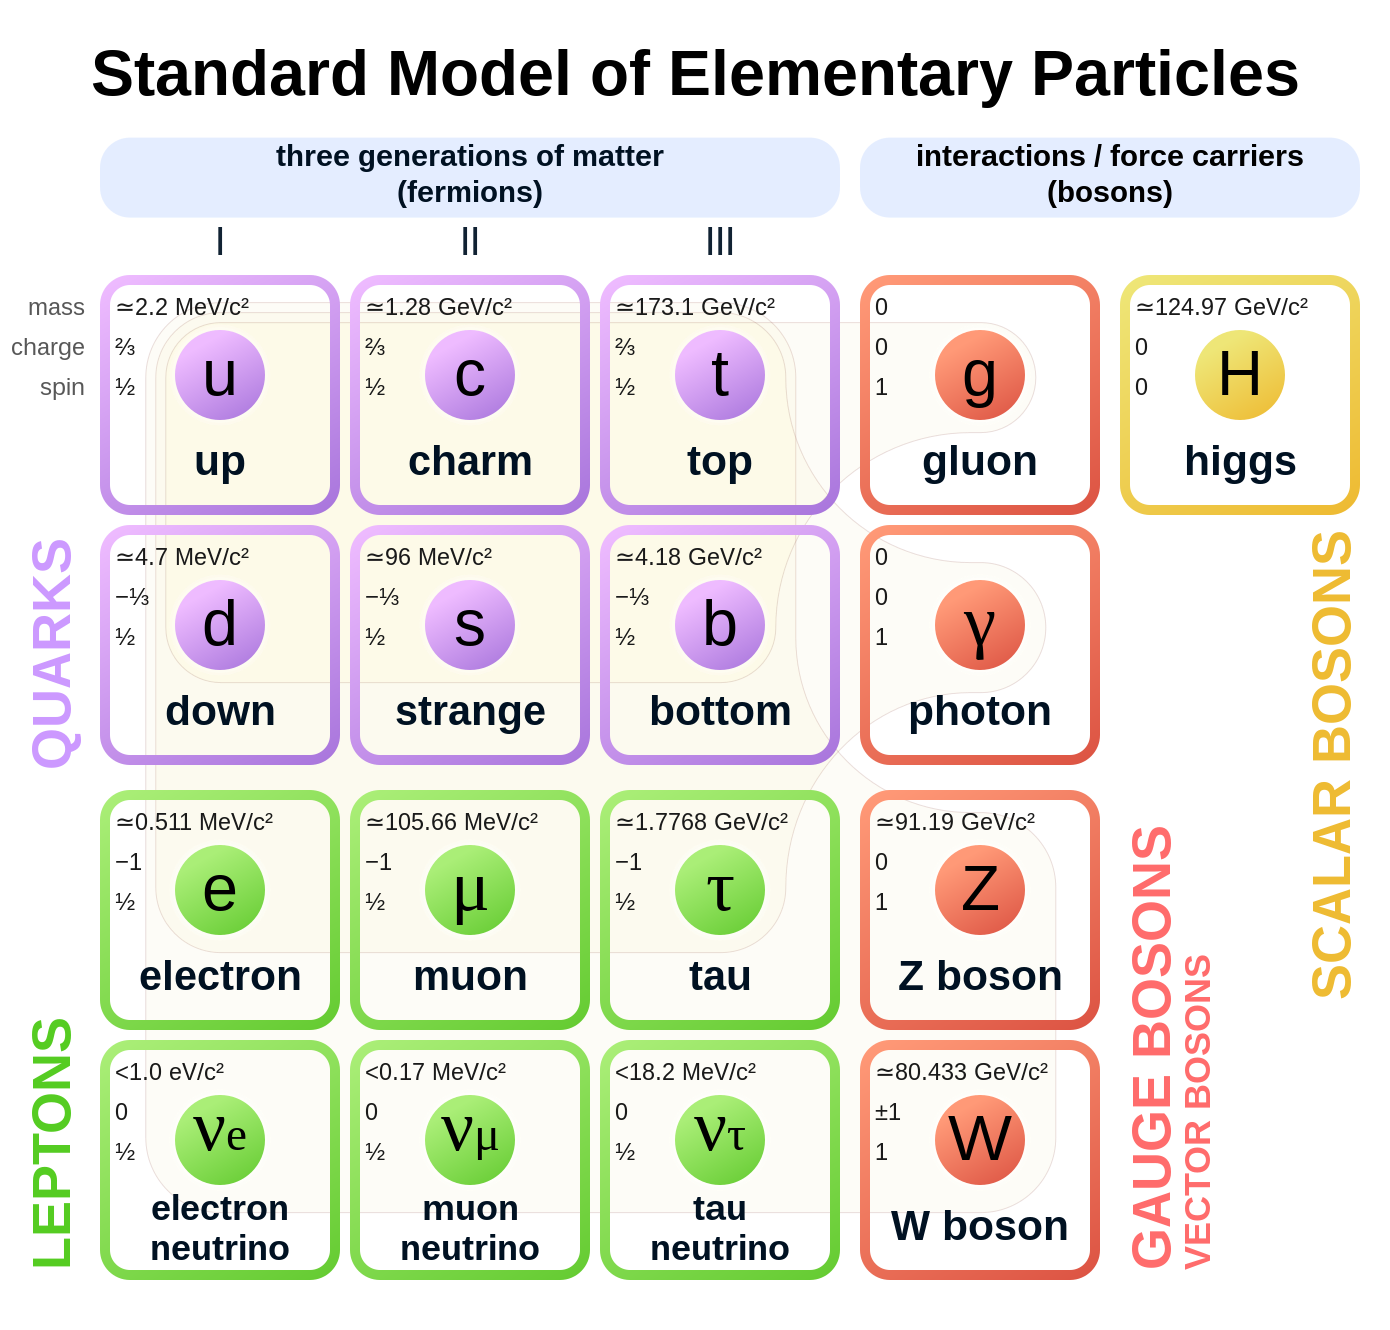
\includegraphics[width=\textwidth]{Figs/Chapter2/Standard_Model_of_Elementary_Particles.svg.png}\label{fig:StdModel}
	\caption{Classification of the elementary particles of the Standard Model, with the fermions on the left and the gauge/scalar bosons on the right. Figure taken from \cite{missmjStandardModelElementary2019}.}
	\label{fig:StdModel}
\end{figure}

Classically, a particle interacts with another via a field (for example, in electromagnetism, a positively charged particle generates an electric field that exerts an attractive/repulsive force on neighboring negative/positive charge). In QFT, fields are quantized, and the energy and momentum previously carried by the field are now conveyed by chunks, by quanta\footnote{Here, we present elementary particles as quanta  of their underlying field as if the particles could be separated/reduced from their field, which corresponds to the usual experimentalist's picture of QFT. In fact, the relation between particles and fields is slightly more subtle \cite{jaegerElementaryParticlesQuantum2021}.} \cite{serwayModernPhysics2004}. So in particle physics, interactions are described as an exchange of quanta or force-carrying particles of spin 1, known as \textit{(vector) gauge bosons}\footnote{They are called \textit{bosons} because, contrarly to the fermions, their intrinsic angular momentum (or spin) has an integer value.}\cite{braibantParticlesFundamentalInteractions2012}\cite{thomsonModernParticlePhysics2013}. Following the remarks in \Sec\ref{subsec:Theory}, the term "(\textit{vector}) \textit{gauge}" emphasizes here the fact that the boson arises from a gauge vector field and therefore a gauge symmetry. 

The most \DIFdelbegin \DIFdel{successful }\DIFdelend \DIFaddbegin \DIFadd{precise }\DIFaddend quantum field theory is the quantum electrodynamics (QED) that describes the interaction between charged particles and electromagnetic fields. It has been developped between 1947 and 1949 by Shin'-ichir$\bar{\text{o}}$ Tomonaga, Julian Schwinger, Richard P. Feynman and Freeman Dyson; only the first three received the 1965 Nobel Prize in Physics for their contributions\footnote{Unfortunately F. Dyson did not receive the Nobel Prize because i) his work was not considered as groundbreaking as the one of the three other laureates and ii) the Nobel Prize in a given field can only be awarded to organisation of maximum of three individuals \cite{schmidhuberEvolutionNationalNobel2010}.}. It is based on a U(1) local gauge symmetry\footnote{U(N) corresponds to the group of all unitary matrices to size $N \times N$. Thus, U(1) is a group containing all the continuous transformations of the phase of a complex number.}, that results into an interaction with charged particles mediated by massless photons. This continuous symmetry is associated to a conserved quantity, namely the electric charge. The dynamics of this interaction is given by the Lagrangian density of QED in \eq\ref{eq:LagrangianQED}.

\begin{equation}
\Lagr_{QED} = \underbrace{i \bar{\psi} \gamma^{\mu} \partial_{\mu} \psi}_{\substack{\text{electron} \\ \text{kinetic term}}} + \underbrace{e \bar{\psi} \gamma^{\mu} A_{\mu} \psi}_{\substack{\text{electron-photon} \\ \text{interaction term}}} - \underbrace{m \bar{\psi} \psi}_{\substack{\text{electron} \\ \text{ mass term}}} - \underbrace{\frac{1}{4} F_{\mu \nu} F^{\mu \nu}}_{\substack{\text{photon} \\ \text{kinetic term}}} 
\label{eq:LagrangianQED}
\end{equation}
where
\begin{itemize}
\item[$\bullet$] $\gamma^{\mu}$ Dirac matrices that express the vectorial nature of the interaction and $\mu$ is the Lorentz vector index,
\item[$\bullet$] $A_{\mu}$ the photon field,
\item[$\bullet$] $F_{\mu \nu} = \partial_{\mu} A_{\nu} - \partial_{\nu} A_{\mu}$ the field-strength tensor,
\item[$\bullet$] $e$ the coupling constant of QED which coincides with the electric charge of the electron-positron field,
\item[$\bullet$] $m$ the electron/positron mass,
\item[$\bullet$] $\psi$ the electron-positron spinor field,
\end{itemize}
with the Einstein's notation $x^{\mu} x_{\mu} = \sum\limits_{\mu=0}^{N} x^{\mu} x_{\mu}$ and the notations from \cite{thomsonModernParticlePhysics2013}.\\

Different terms appear in the expression of the Lagrangian density: the \DIFaddbegin \DIFadd{density of }\DIFaddend kinetic energy of the spinor field, the \DIFaddbegin \DIFadd{density of }\DIFaddend potential energy due to the interaction between the spinor and gauge fields, the mass energy of the spinor field\footnote{If the gauge boson is massive, there would be an extra mass term. Since the photon is massless, this term is null.}, the \DIFaddbegin \DIFadd{density of }\DIFaddend kinetic energy of the gauge boson (photon). The most interesting term is the second one, which describes the interaction between the charged particles and the photons. This interaction gives rise to different processes, usually pictured by Feynman diagrams. \Fig\ref{fig:FeynmanDiagramQED} shows the basic interaction vertex in QED.

\begin{figure}[H]
\begin{center}
\unitlength = 1mm
\subfigure[]{
	\begin{fmffile}{eegamma}
	\begin{fmfgraph*}(40,25)
	\fmfleft{i1,i2}
	\fmfright{o1}
	\fmflabel{$e^{-}$}{i1}
	\fmflabel{$e^{+}$}{i2}
	\fmf{fermion}{i1,v1}
	\fmf{fermion}{v1,i2}
	\fmf{photon,label=$\gamma$}{v1,o1}
	\end{fmfgraph*}
	\end{fmffile}
	\label{fig:eegamma}
}
\subfigure[]{
	\begin{fmffile}{lqlqgamma}
	\begin{fmfgraph*}(40,25)
	\fmfleft{i1,i2}
	\fmfright{o1}
	\fmflabel{$l, q$}{i1}
	\fmflabel{$\bar{l}, \bar{q}$}{i2}
	\fmf{fermion}{i1,v1}
	\fmf{fermion}{v1,i2}
	\fmf{photon,label=$\gamma$}{v1,o1}
	\end{fmfgraph*}
	\end{fmffile}
	\label{fig:lqlqgamma}
}
\end{center}
\caption{Interaction vertex in QED: (a) involving an electron and a positron, (b) generalized to any charged particles.}
\label{fig:FeynmanDiagramQED}
\end{figure}



Being the first quantum field theory developed, QED paved the way -- and even served as a template -- for all the subsequent quantum field theories. Therefore, it is not surprising that the form of Lagrangian density is the same for all the forces. 

Following the success of QED, attempts to develop a quantum field theory for the weak interaction started in the 1950s; none of them could provide a satisfactory description. In the same decade, important discoveries have been made: the Wu's\footnote{Awarded of the 1957 Nobel Prize.} (1956) and Goldhaber's (1957) experiments \cite{wuExperimentalTestParity1957}\cite{goldhaberHelicityNeutrinos1958} showed that the P- and CP-symmetries are violated by the weak interaction. These led to conclude that this force has a vector-axial vector structure, meaning that only interacts with left-handed chiral particles and right-handed chiral anti-particles. Meanwhile, a few physicists -- including \DIFdelbegin \DIFdel{Schwinger, his PhD students }\DIFdelend \DIFaddbegin \DIFadd{Abdus Salam, Steven Weinberg, Schwinger and his PhD student }\DIFaddend Sheldon L. Glashow \DIFdelbegin \DIFdel{, Abdus Salam and Steven Weinberg }\DIFdelend -- foresaw that the weak and electromagnetic forces might be two aspects of the same phenomenon. Thanks to the work of Chen Ning Yang and Robert Mills on the development of a generalized gauge theory in 1954, Glashow delivered the electroweak interaction in 1961, which was consolidated later in 1967 and 1968 by Weinberg and Salam\footnote{For their contribution, Glashow, Salam and Weinberg receive the 1979 Nobel Prize.} respectively. In this quantum field theory, the electromagnetic and weak forces are described within an unified framework; the weak interaction is based on the SU(2) gauge group\footnote{The S (for "special") refers to the group of all matrices whose determinant is equal to 1.}, three generators hence three gauge bosons: \rmWplus, \rmWminus and \rmZzero. These bosons exhibit two unique properties.  First, contrarly to all other gauge bosons, these ones have an enormous mass (m$_{\textrm{W}^{\pm}}$ = 80.377 \gmass and m$_{\textrm{Z}^{0}}$ = 91.1876 \gmass \DIFdelbegin \DIFdel{\mbox{%DIFAUXCMD
\cite{particledatagroup2022}}\hspace{0pt}%DIFAUXCMD
}\DIFdelend \DIFaddbegin \DIFadd{\mbox{%DIFAUXCMD
\cite{particledatagroupReviewParticlePhysics2022}}\hspace{0pt}%DIFAUXCMD
}\DIFaddend ), which explains why the weak force is such a short-range interaction. Second, the \rmWplusminus bosons can change the flavour of quarks and leptons. The trend (or the probability) of the flavour-changing is given by the \textbf{C}abibbo-\textbf{K}obayashi-\textbf{M}askawa\footnote{The Universe is unfair: similarly to Dyson for the QED, Nicolas Cabibbo (the pioneer of the CKM matrix) was not awarded with the 2008 Nobel Prize, while Makoto Kobayashi and Toshihide Maskawa were.} (CKM) matrix \cite{particledatagroupReviewParticlePhysics2022}\footnote{Mathematically speaking, this matrix relates the mass eigenstates to the weak eigentstates \cite{thomsonModernParticlePhysics2013}.} in \eq\ref{eq:CKMmatrix}.

\begin{equation}
V_{\textrm{CKM}} = 
\begin{pmatrix}
V_{\rm ud} & V_{\rm us} & V_{\rm ub}\\
V_{\rm cd} & V_{\rm cs} & V_{\rm cb}\\
V_{\rm td} & V_{\rm ts} & V_{\rm tb}
\end{pmatrix} = 
\begin{pmatrix}
0.97425 \pm 0.00022 & 0.2253 \pm 0.0008 & 0.00413 \pm 0.00049\\
0.225 \pm 0.008 & 0.986 \pm 0.016 & 0.0411 \pm 0.0013\\
0.0084 \pm 0.0006 & 0.040 \pm 0.0027 & 1.021 \pm 0.032
\end{pmatrix}\label{eq:CKMmatrix}
\end{equation}

Each matrix element provides the probability of transition from one flavour $i$ to another $j$ for quarks, but the same exists for the leptons and is called the \textbf{P}ontecorvo-\textbf{M}aki-\textbf{N}akagawa-\textbf{S}akata (PMNS) matrix. The elements of the PMNS matrix are slightly different from the CKM ones, though the structure and ordering are the same. 

Finally, concerning the strong interaction, we will see later in its dedicated sub-section, \Sec\ref{subsec:strongforce}. Patience!
\\


The overall picture of the Standard Model's elementary particles is presented in \fig\ref{fig:StdModel}. To this figure should be added the antiparticles. Indeed, to each particle -- fermion or boson -- \DIFdelbegin \DIFdel{, there }\DIFdelend corresponds an antiparticle that \DIFdelbegin \DIFdel{have }\DIFdelend \DIFaddbegin \DIFadd{has }\DIFaddend the same properties, because of the CPT invariance, but with oppositely sign quantum numbers. Consequently, this also means that both CKM and PMNS matrices are the same for particles and antiparticles.

There is, however, one element of the table in the \fig\ref{fig:StdModel} that has not been discussed yet, that is the Higgs boson. It originates from the electroweak unification, so let us retrace our footsteps. The principles of gauge invariance inevitably give rise to massless gauge bosons, like the photons but not the massive \rmWplusminus, \rmZzero bosons. At the time of Glashow's electroweak model in 1961, no one could imagine a mechanism to generate the enormous masses of the weak interaction force-carriers. In the same year, Jeffrey Goldstone showed that the process of spontaneous symmetry breaking\footnote{This is the phenomenon in which a physical system perfectly symmetric breaks the symmetry without any external intervention. The most famous example of such process concerns the magnets. A material can be seen as an ensemble of microscopic magnets. If this material is ferromagnetic, all these magnets will tend to align with their neighbors.  When the temperature increases, the thermal motions start to disrupt this alignement until the material is not magnetized anymore. Conversely, as the material cools down, neighboring magnets starts to align until a critical temperature, when all the magnets lines up in one macroscopic direction. All directions are equivalent but the magnet has to choose one. This choice breaks the symmetic situation when all the directions are equivalent; this is a \textit{symmetry breaking}. Moreover, this choice is not influenced by any external agent, hence it is labelled as \textit{spontaneous}.\label{footnote:SpontaneousSymmetryBreaking}} leads to the existence of massless gauge bosons, called Goldstone bosons. Three years later, in 1964, three independent groups (Robert Brout and François Englert; Peter Higgs; Gerald Guralnik, Carl Richard Hagen, and Tom Kibble) demonstrated the Goldstone bosons could be absorbed by the massless gauge bosons to acquire a mass: this is the Higgs mechanism. It is only in 1967-68, that Weinberg and Salam put to use this mechanism within Glashow's model to generate the masses of \rmWplusminus and \rmZzero bosons. But this goes beyond the scope of the electroweak unification; with this \DIFdelbegin \DIFdel{process is generated }\DIFdelend \DIFaddbegin \DIFadd{mechanism, }\DIFaddend the mass of all elementary particles \DIFaddbegin \DIFadd{can be generated }\DIFaddend \cite{s.glashowInteractionsJourneyMind1990}. Incidentally, a new massive spinless particle, associated to a scalar field, \DIFdelbegin \DIFdel{is introduced }\DIFdelend \DIFaddbegin \DIFadd{emerges }\DIFaddend out of the Higgs mechanism: the Higgs boson. Its observation in laboratory was at the heart of Standard Model \DIFdelbegin \DIFdel{research }\DIFdelend \DIFaddbegin \DIFadd{researches }\DIFaddend for decades until the \DIFdelbegin \DIFdel{8th of October }\DIFdelend \DIFaddbegin \DIFadd{14th of March }\DIFaddend 2013 when the ATLAS and CMS experiments at the LHC at CERN announced the discovery of the Higgs boson \DIFaddbegin \DIFadd{\mbox{%DIFAUXCMD
\cite{cernNewResultsIndicate2023}}\hspace{0pt}%DIFAUXCMD
\mbox{%DIFAUXCMD
\cite{kibbleEnglertBroutHiggsGuralnikHagenKibbleMechanismHistory2009}}\hspace{0pt}%DIFAUXCMD
}\DIFaddend . The same year, Peter Higgs and François Englert receive the Nobel Prize for their contribution to the Standard Model.


\subsection{The strong force, a colourful interaction}
\label{subsec:strongforce}

Back in the 1960s, in the \DIFdelbegin \DIFdel{"glorious years" }\DIFdelend \DIFaddbegin \say{glorious years} \DIFaddend of particle physics, when physicists were submerged by the number of newly discovered \DIFdelbegin \DIFdel{"elementary" }\DIFdelend \DIFaddbegin \say{elementary} \DIFaddend particles. Some of them were subject to the strong interaction, some were not; the former were \DIFdelbegin \DIFdel{refered }\DIFdelend \DIFaddbegin \DIFadd{referred }\DIFaddend as \textit{hadrons}\footnote{The expression originates from the Greek \textit{adros} meaning "thick and bulky".} and the latter as \textit{leptons}, as discussed in \Sec\ref{subsec:ParticleAndInteractions}. The hadrons were further sorted into two groups known as \textit{mesons} and \textit{baryons}\footnote{These terms originally refer to the mass of the particle: \textit{meson} comes from the Greek root \textit{meso} for "middle", that is in between the electron and proton masses; \textit{baryon} stem from Greek \textit{barys} for "heavy", suggesting any particle with a mass greater or similar to the one of the nucleons. Before the development of the quark model, the difference between the meson and the baryon was driven by their spin. The meson is a boson (integer spin values) where as the baryon is a fermion (half-integer spin values)\cite{s.glashowInteractionsJourneyMind1990}.}. But no one could draw out the underlying scheme between these particles and organise them into some kind of periodic table. There were some attempts though \cite{sakataCompositeModelNew1956}\cite{sakuraiTheoryStrongInteractions1960}; however the Mendeleev of particle physics is arguably Murray Gell-Mann. 

In 1961, he (and independently Yuval Ne'eman) proposed a classification scheme called the \textit{eightfold way} \cite{gell-mannEIGHTFOLDWAYTHEORY1961}\cite{neemanDerivationStrongInteractions1961}. At that time, eight spinless mesons, eight vector mesons of spin 1 and eight spin 1/2 baryons were known. In each of these octets, a pattern emerges when the hadrons are organized into groups/multiplets of roughly the same mass, a hint of the underlying structure of strong interaction. A year later, the eightfold way is updated and completed with a decuplet formed of spin-$\frac{3}{2}$ baryons. However, one of the ten members of the decuplet was not yet discovered but this periodic table of elementary particles can predict its properties: a mass near the 1675 \mmass, strangeness\footnote{A quantum number introduced by Murray Gell-Mann in 1953 order to explain the \textit{strange} behaviour of some particles, such as kaons \cite{gell-mannIsotopicSpinNew1953}. Any particle with a non-zero strangeness value is dubbed \textit{strange particle}.} of -3 and negatively charged, these are the characteristics of the \rmOmegaM. Its existence is confirmed experimentally in 1964 by the Alternating Gradient Synchrotron at the Brookhaven National Laboratory (BNL)\cite{barnesObservationHyperonStrangeness1964a}, validating the eightfold way once and for all.\\

Within the year of this discovery, Murray Gell-Mann (and independently Georges Zweig) unveiled the symmetry behind the eightfold way: there are no elementary hadrons; they are, in fact, all built out of more fundamental particles named \textit{quarks}. A composite object made of bosons can only lead to a boson whereas, formed by fermions, the object is either a fermion or a boson depending on the number of constituents involved. Hence, the quarks must be fermions of spin one-half, mesons are composed of an even number of quarks, baryons of an odd number. The smallest odd number is one, but i) it does not make sense to say that a composite structure is made of one constituent and ii) we will see later in \Sec\ref{subsubsec:confinement} that a system of one quark is physically impossible. Thus, mesons must be made out of two quarks and baryons out of three; these are the simplest imaginable arrangements. 

Originally, quarks exist in two flavours, \textit{up} ($u$) and \textit{down} ($d$), with fractional electric charges of $+2e/3$ and $-1e/3$ respectively. \DIFdelbegin \DIFdel{An }\DIFdelend \DIFaddbegin \DIFadd{But an }\DIFaddend extra flavour was needed to explain the existence of strange hadrons: the strange quark, $s$, is born. It has the same properties as the $d$ quark, except that it is much heavier and it has an assigned strangeness number of -1. Any strange hadrons actually contains one to three $s$ quark, depending on their strangeness. Therefore, the predicted particle by the eightfold way, the \rmOmegaM, corresponds actually to the strangest hadron possible, a baryon with three strange quarks. 

With this particle comes the first difficulty of the quark model. Whatever the particle, it must obey the spin-statistics theorem. Quarks being fermions, the theorem states that two \textit{identical} fermions can not occupy the same quantum states simultaneously. However, \rmOmegaM is constituted of three exactly identical $s$-quark \cite{skandsIntroductionQCD2013}. This problem was overcome by Oscar W. Greenberg \cite{greenbergSpinUnitarySpinIndependence1964}, Moo-Young Han and Yoichiro Nambu \cite{hanThreeTripletModelDouble1965} in 1964-65 that introduced a new quantum number, the colour. Each quark comes in three colours or variants labelled as red ($r$), green ($g$) and blue ($b$). In this way, the spin-statistics problem is solved but new questions arises. If quarks carry a colour, hadrons are a mixture of colours. This is assumed to be an equal mixture of all the colours, such that the hadrons are colourless. How come? Why are there no coloured hadrons? 

Along the same line: in 1966, the main accelerator at the Stanford Linear Accelerator Center (SLAC) becomes operational and starts a program of deep inelastic scattering experiments in order to study the inner structure of nucleons. Based on James Bjorken\DIFaddbegin \DIFadd{'s }\DIFaddend \cite{bjorkenCurrentAlgebraSmall2018} and Richard Feynman\DIFaddbegin \DIFadd{'s  }\DIFaddend \cite{feynmanBehaviorHadronCollisions1988} calculations, the results of SLAC's experiments, in 1969, showed that the nucleons were made of point-like constituents of spin-$\frac{1}{2}$, dubbed \textit{partons}, behaving as free particles \cite{peskinIntroductionQuantumField2018}. The partons were nothing else than the quarks, and these observations established the validity the quark picture to the whole particle physics community. However, it is curious that the partons seem to behave as free particles but they can not escape the hadron.\\

These questions remain unanswered until 1973. This year had seen the development of Quantum Chromodynamics (QCD) -- the quantum field theory of the strong force -- and the discovery of two of its most salient properties, namely the colour confinement and the asymptotic freedom (discussed in \Sec\ref{subsubsec:confinement}). Fruit of the work of Harald Fritzsch, Heinrich Leutwyler and Murray Gell-Mann \cite{fritzschAdvantagesColorOctet1973}, the QCD describes the interaction between colour-charged objects, namely the partons. It is based on the gauge symmetry group SU(3), which has eight generators, giving rise to eight massless gauge bosons called \textit{gluons}, and imposes the conservation of colour. 

QCD is very similar to QED: the electric charge is replaced by a colour charge, antiparticles carry opposite colour charges, and the eight gluons take the role of the photon. The dynamics of QCD is given by the Lagrangian density in \eq\ref{eq:LagrangianQCD}.\\

\begin{equation}
\Lagr_{QCD} = \underbrace{i \bar{\psi}_{q}^{i} \gamma^{\mu} \delta_{ij} \partial_{\mu} \psi_{q}^{j}}_{\substack{\text{quark} \\ \text{kinetic term}}} + \underbrace{g_{s} \bar{\psi}_{q}^{i} \gamma^{\mu} t_{ij}^{a} A_{\mu}^{a} \psi_{q}^{j}}_{\substack{\text{quark-gluon} \\ \text{interaction term}}} - \underbrace{m_{q} \bar{\psi}_{q}^{i} \psi_{qi}}_{\substack{\text{quark} \\ \text{mass term}}} - \underbrace{\frac{1}{4} F_{\mu \nu}^{a} F^{a \mu \nu}}_{\substack{\text{gluon} \\ \text{kinetic term}}} 
\label{eq:LagrangianQCD}
\end{equation}
where, using the notations from \cite{skandsIntroductionQCD2013},
\begin{itemize}
\item[$\bullet$] $g_s^2 = 4 \pi \alpha_s$ with \alphaS the coupling constant of QCD,
\item[$\bullet$] $F_{\mu \nu}^{a} = \underbrace{\partial_{\mu} A_{\nu}^{a} - \partial_{\nu} A_{\mu}^{a}}_{\text{Abelian part}} + \underbrace{g_{s} f^{abc} A_{\mu}^{b} A_{\nu}^{c}}_{\text{non-Abelian part}}$ the field-strength tensor,
\item[$\bullet$] $\psi_{q}^{i}$ the quark field spinor with colour index $i$ such that $\psi_{q} = \left({\color{red}\psi_{qR}}, {\color{green}\psi_{qG}}, {\color{blue}\psi_{qB}} \right)^{\rm T} $,
\item[$\bullet$] $m_{q}$ the quark \textit{bare} mass induced by the Higgs mechanism,
\item[$\bullet$] $A_{\mu}^{a}$ the gluon field with colour index $a$,
\item[$\bullet$] $t_{ij}^{a} = \frac{1}{2} \lambda_{ij}^{a}$ and $\lambda^{a}$ the fundamental\footnote{The representation of a group is \textit{fundamental} when its generators are hermitian and traceless matrices. } representation of the generator of SU(3) associated to the colour index $a$,
\item[$\bullet$] $f^{abc}$ the structure constants of SU(3).\\
\end{itemize}

As in QED, the Lagrangian density can be expressed with four terms; the quark-gluon interaction is described by the second one. However, the field-strength tensor $F_{\mu \nu}^{a}$ here admits an extra term because the generators of SU(3) do not commute. The non-Abelian property of the gauge group of QCD gives rise to gluon-self interactions, as shown in the Feynman's diagrams of \fig\ref{fig:FeynmanDiagQCD}.

\begin{figure}[H]
\begin{center}
\unitlength = 1mm
\subfigure[]{
	\begin{fmffile}{qqg}
	\begin{fmfgraph*}(40,25)
	\fmfleft{i1,i2}
	\fmfright{o1}
	\fmflabel{$q$}{i1}
	\fmflabel{$\bar{q}$}{i2}
	\fmf{fermion}{i1,v1}
	\fmf{fermion}{v1,i2}
	\fmf{gluon,label=$g$, lab.dist=0.1w}{v1,o1}
	\end{fmfgraph*}
	\end{fmffile}
	\label{fig:qqg}
}
\subfigure[]{
	\begin{fmffile}{ggg}
	\begin{fmfgraph*}(40,25)
	\fmfleft{i1,i2}
	\fmfright{o1}
	\fmflabel{$g$}{i1}
	\fmflabel{$g$}{i2}
	\fmflabel{$g$}{o1}
	\fmf{gluon}{i1,v1}
	\fmf{gluon}{i2,v1}
	\fmf{gluon}{v1,o1}
	\fmfv{lab=$g_s$,lab.dist=0.15w}{v1}
	\fmfdot{v1}
	\end{fmfgraph*}
	\end{fmffile}
	\label{fig:ggg}
}
\subfigure[]{
	\begin{fmffile}{gggg}
	\begin{fmfgraph*}(40,25)
	\fmfleft{i1,i2}
	\fmfright{o1,o2}
	\fmflabel{$g$}{i1}
	\fmflabel{$g$}{i2}
	\fmflabel{$g$}{o1}
	\fmflabel{$g$}{o2}
	\fmf{gluon}{i1,v1}
	\fmf{gluon}{i2,v1}
	\fmf{gluon}{v1,o1}
	\fmf{gluon}{v1,o2}
	\fmfv{lab=$g_s^2$,lab.dist=0.15w}{v1}
	\fmfdot{v1}
	\end{fmfgraph*}
	\end{fmffile}
	\label{fig:gggg}
}
\end{center}
\caption{The three possible interaction vertices within the framework of QCD: (a) quark-gluon, (b) triple-gluon and (c) four-gluon interactions.}
\label{fig:FeynmanDiagQCD}
\end{figure}

Consequently to the self-interaction of QCD's force-carriers, gluons can not be colour neutral. To ensure colour conservation at the interaction vertex in \fig\ref{fig:qqg}, the gluon must carry a colour and an anti-colour charges. This calls for a revision of the term \textit{partons}: it corresponds to any colour-charged elementary particle, that is the quarks \textit{and} gluons. 

Furthermore, quarks are bound together inside hadrons through the exchange of gluons, but because of their self-interaction feature, gluons can radiate other gluons (\fig\ref{fig:ggg}); the latters can, in turn, split into a quark-antiquark pair (\fig\ref{fig:qqg}) or emit gluons again, and so on. The static picture of hadrons  with two or three quarks exchanging gluons turns out to be more complex, permeated in a \textit{sea} of quarks (and antiquarks) and gluons\footnote{An effect of the sea of quarks and gluons is the Bjorken scaling violation observed by the HERA experiment \cite{braibantParticlesFundamentalInteractions2012}\cite{thomsonModernParticlePhysics2013}.}. However, the elements inside the sea do not determine the quantum numbers or properties of the hadron, as opposed to the "original" quarks; for this reason, the latter are often refered as \textit{valence quarks}.

Finally, an incidental consequence of gluon's self-interaction is the running of the coupling constant. This can be understood by making a (anti)parallel with QED. Let us say we want to measure the coupling strength with a charged particle (an electron, for example). In QFT, the vacuum is not entirely empty, it contains \DIFdelbegin \DIFdel{pair }\DIFdelend \DIFaddbegin \DIFadd{pairs }\DIFaddend of particles and antiparticles that are constantly created and annihilated. Such a pair can also be formed by the cloud of \textit{virtual}\footnote{Certainly the most vague concept in particle physics. It appears in perturbation theory (see later) and an attempt for a definition could be: it corresponds to a theoretical particle wich exhibits the same properties as ordinary particles but not \DIFdelbegin \DIFdel{necessarly }\DIFdelend \DIFaddbegin \DIFadd{necessarily }\DIFaddend (for example, they do not satisfy the energy-momentum relation), and with a lifetime so short that it could never be observed experimentally.} photons surrounding the charged particle to be tested; in this case, it is said to \textit{polarise the vacuum}. An example of this process can be found in \fig\ref{fig:ChargeScreening}. The positively charged particle from the vacuum is attracted to the initial electron, leading in a screening effect similar to the one found in a dielectric material (\fig\ref{fig:Dielectric}). At large distance (or small energy), it is more difficult to penetrate inside the cloud of virtual particle-antiparticle pairs and to probe the initial charge, reducing the coupling strength. Conversely, at small distance (or large energy), the initial charge can be distinguished from the surrounding positively charged particles and the coupling strengthen. In QCD, the opposite happens.  Because gluons carry a colour charge, the initial colour of the particle to be tested (a quark) gets spread out, as depicted in \fig\ref{fig:ColourSpread}. Thus, an anti-screening effect occurs: the initial red-coloured quark spends most of its time coloured as blue or green, and the red colour charge is diluted in the surrounding cloud of partons. At large distance (or small energy), the initial quark $r$ is overly apparent for an incoming gluon $\bar{r}g$ or $\bar{r}b$; conversely, at small distance (large energy), the initial red quark -- likely converted into a green or blue quark -- is invisible to such a gluon, resulting in a weakening of the coupling strength. \\

\begin{figure}[t]
\begin{center}
\subfigure[]{
	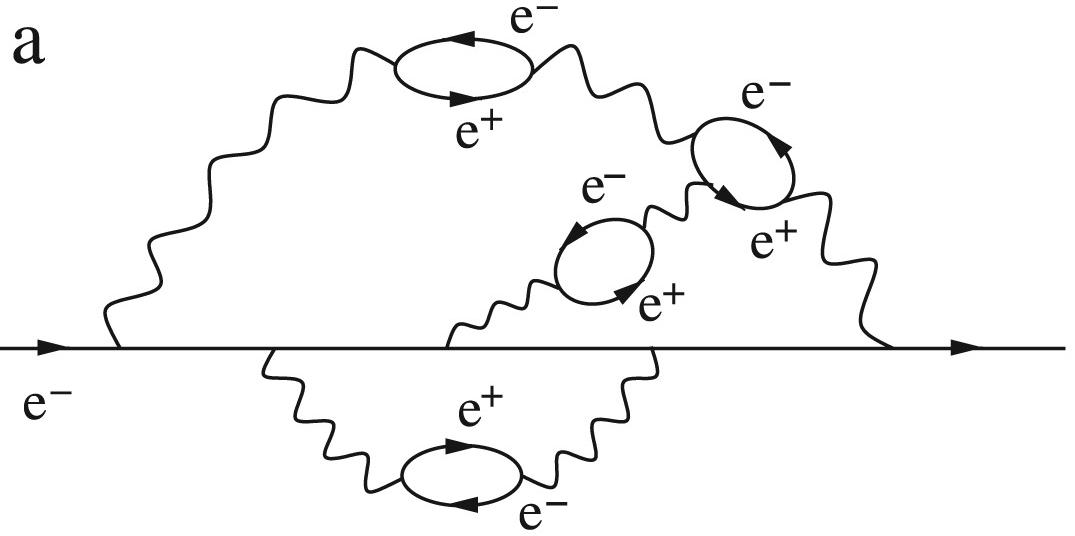
\includegraphics[height=0.25\textwidth]{Figs/Chapter2/1-s2.0-S0146641016300035-gr2_lrg}
	\label{fig:ChargeScreening}
}
\subfigure[]{
	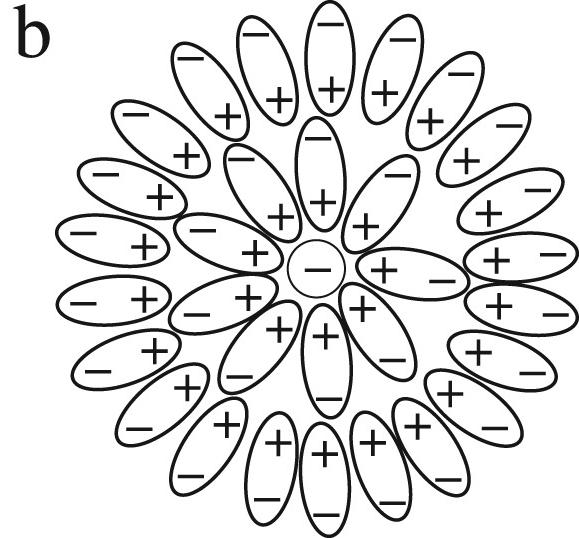
\includegraphics[height=0.25\textwidth]{Figs/Chapter2/1-s2.0-S0146641016300035-gr2bis_lrg}
	\label{fig:Dielectric}
}
\subfigure[]{
	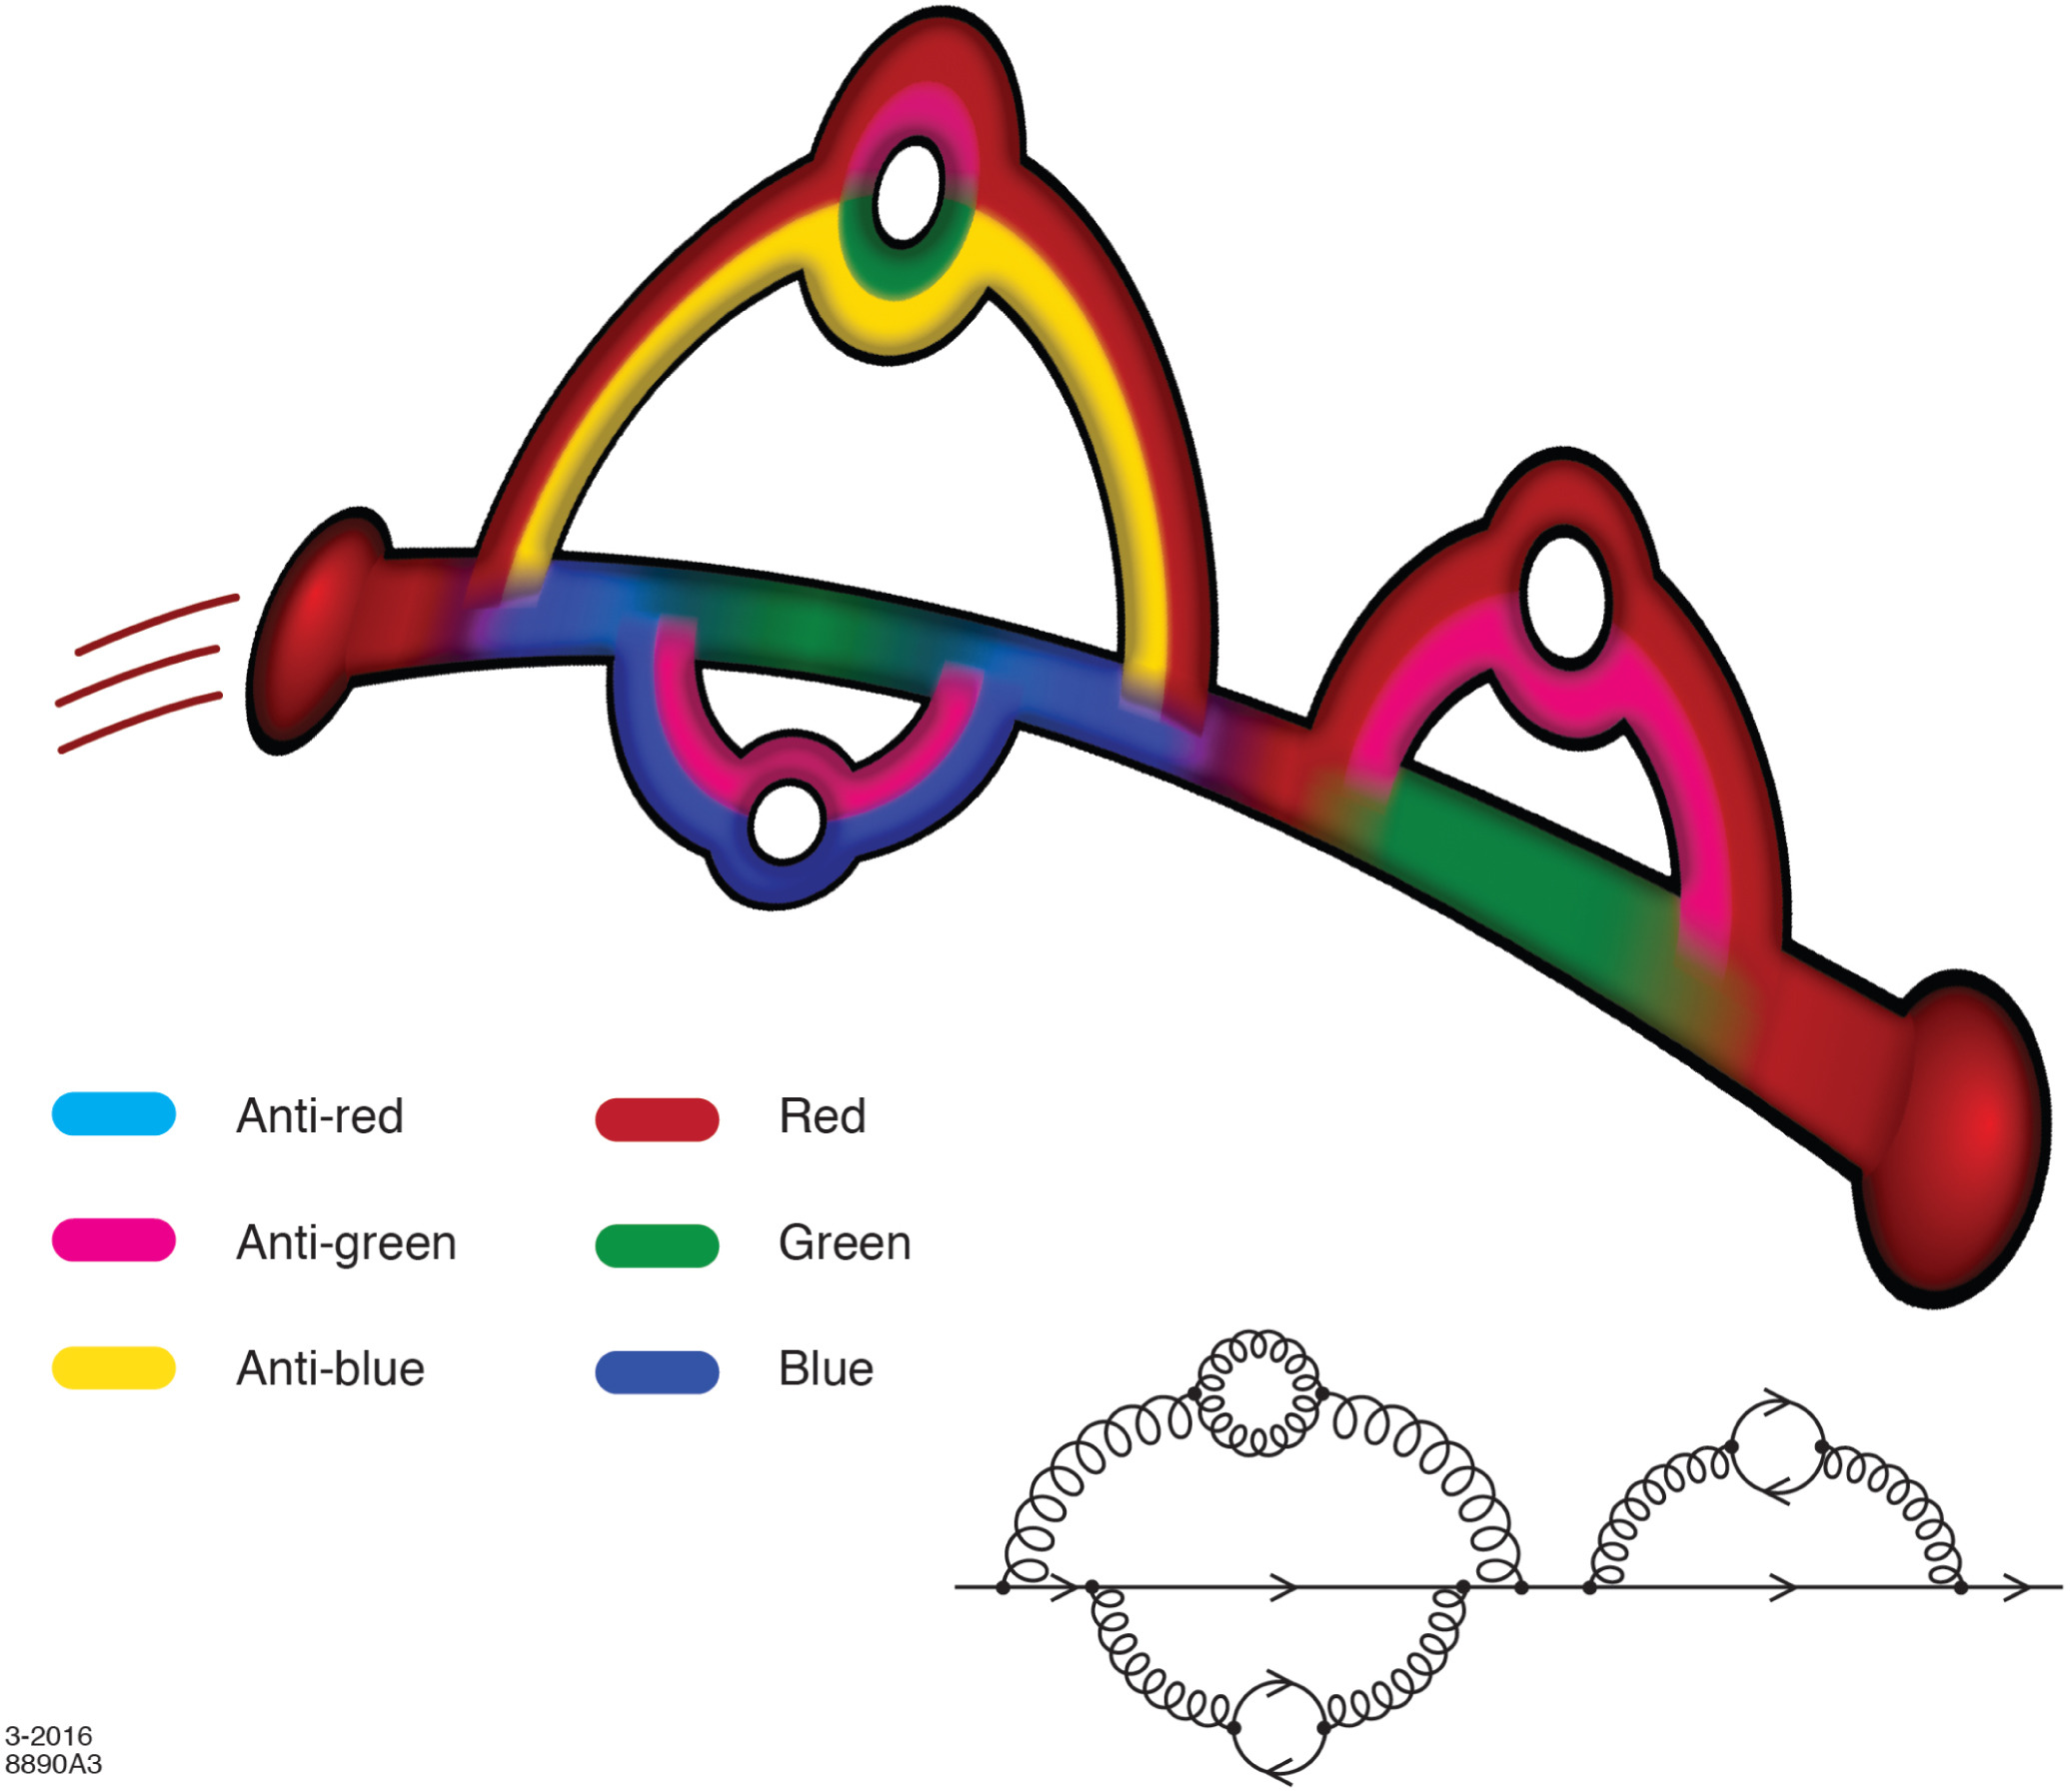
\includegraphics[width=0.8\textwidth]{Figs/Chapter2/1-s2.0-S0146641016300035-gr1_lrg.jpg}
	\label{fig:ColourSpread}
}
\end{center}
\caption{(a) screening effect of an electron in QED, induced ;(b) analogy with the screening effect in a dielectric material; (c) pictural representation of the colour spread of an initially red coloured quark. }
\label{fig:ProbingTestCHarge}
\end{figure}

%A physical picture often used to describe this effect is that a charged particle "polarizes the vacuum", and is "dressed" by a cloud of virtual photons and other charged particles. An electron will attract virtual positively charged particles out of the vacuum that effective screen the electric charge seen by an observer far away from the electron, reducing the size of the coupling. By bringing two charged particles to shorter distances (so they interact at a higher energy), the effective coupling between them is stronger because each charge penetrates the other's cloud, and so the virtual particles swarming in the quantum vacuum are less able to screen the bare charge of each charged particle. The reason for the name "screening" is that (in this picture) the quantum vacuum is screening the bare charge by surrounding it with virtual particles of the opposite charge. I should emphasize that this is a nice physical picture, but ultimately is just a set of words draped around a rigorous calculation of the running of the electromagnetic coupling with energy.

Before continuing, allow me to digress and finish with the different quarks within the \DIFdelbegin \DIFdel{framework QCD }\DIFdelend \DIFaddbegin \DIFadd{QCD framework}\DIFaddend . The alert reader may have guessed that the story did not end with the strange quark. In 1964, James Bjorken and Sheldon Glashow introduced a new quark flavour: the charm quark. It is motivated by the idea of a quark-lepton symmetry\footnote{The term \textit{charm} is chosen for designating this fourth flavour because the definition found by Bjorken and Glashow in \textit{American Heritage Dictionnary}: "an action or formula thought to have magical power", implying magical power to restore the quark-lepton symmetry \cite{s.glashowInteractionsJourneyMind1990}.} at that time, there was four known leptons (electron, muon and their associated neutrinos) and three quarks. But the charm quark definitely comes into play in 1970 by Sheldon Glashow (again), John Iliopoulos and Lucinao Maiani to explain the strangeness-changing neutral currents\footnote{This is typically the case of the decay of a negative kaon to a negative pion with a neutrino and an anti-neutrino ($\rmKminus \rightarrow \piMinus \nu \bar{\nu}$). It is called a strangeness-changing neutral current because i) the strange particle (kaon) changed into an ordinary one (pion), and ii) there is no electric (or neutral) charge transfer between the hadrons to the leptons. This process was never observed in laboratory, as opposed to the strangeness-changing charged current: ($\rmKminus \rightarrow \piZero e^{-} \bar{\nu}_{e}$). To eliminate the strangeness-changing neutral currents, a new quark flavour needed to be introduced \cite{s.glashowInteractionsJourneyMind1990}.}. Its existence is validated by the observation of the first charmed hadron in 1974 by Burton Richter (SLAC)\cite{augustinDiscoveryNarrowResonance1974} and Samuel Chao Chung Ting (BNL)\cite{aubertExperimentalObservationHeavy1974}; both receive the 1976 Nobel Prize for that discovery. In parallel, a third generation of quark is introduced, in 1972 by Makoto Kobayashi and Toshihide Maskawa\footnote{For the discovery of, at least, a third family of quarks, they both receive the 2008 Nobel Prize.} to explain the observed CP violation. The particles composing this new family make their appearence in 1975, thanks to Haim Harari \cite{harariNewQuarkModel1975}, under the name of \textit{bottom} and \textit{top} quarks\footnote{Both belong to the same weak isospin doublet, as are the down and up quarks. To match the labelling of the first generation of quarks, the names \textit{bottom} and \textit{top} were chosen.}. Evidence of the bottom quark is found in 1977 by Leon M. Lederman at Fermilab \cite{herbObservationDimuonResonance1977}. Due to its large mass, the discovery of the top quark takes more time but ultimately occurs in 1995 by two groups at Fermilab \cite{cdfcollaborationObservationTopQuark1995}\cite{d0collaborationObservationTopQuark1995}.

\subsubsection{Running of \alphaS, colour confinement and asymptotic freedom}
\label{subsubsec:confinement}

\begin{figure}[h]
	\centering
	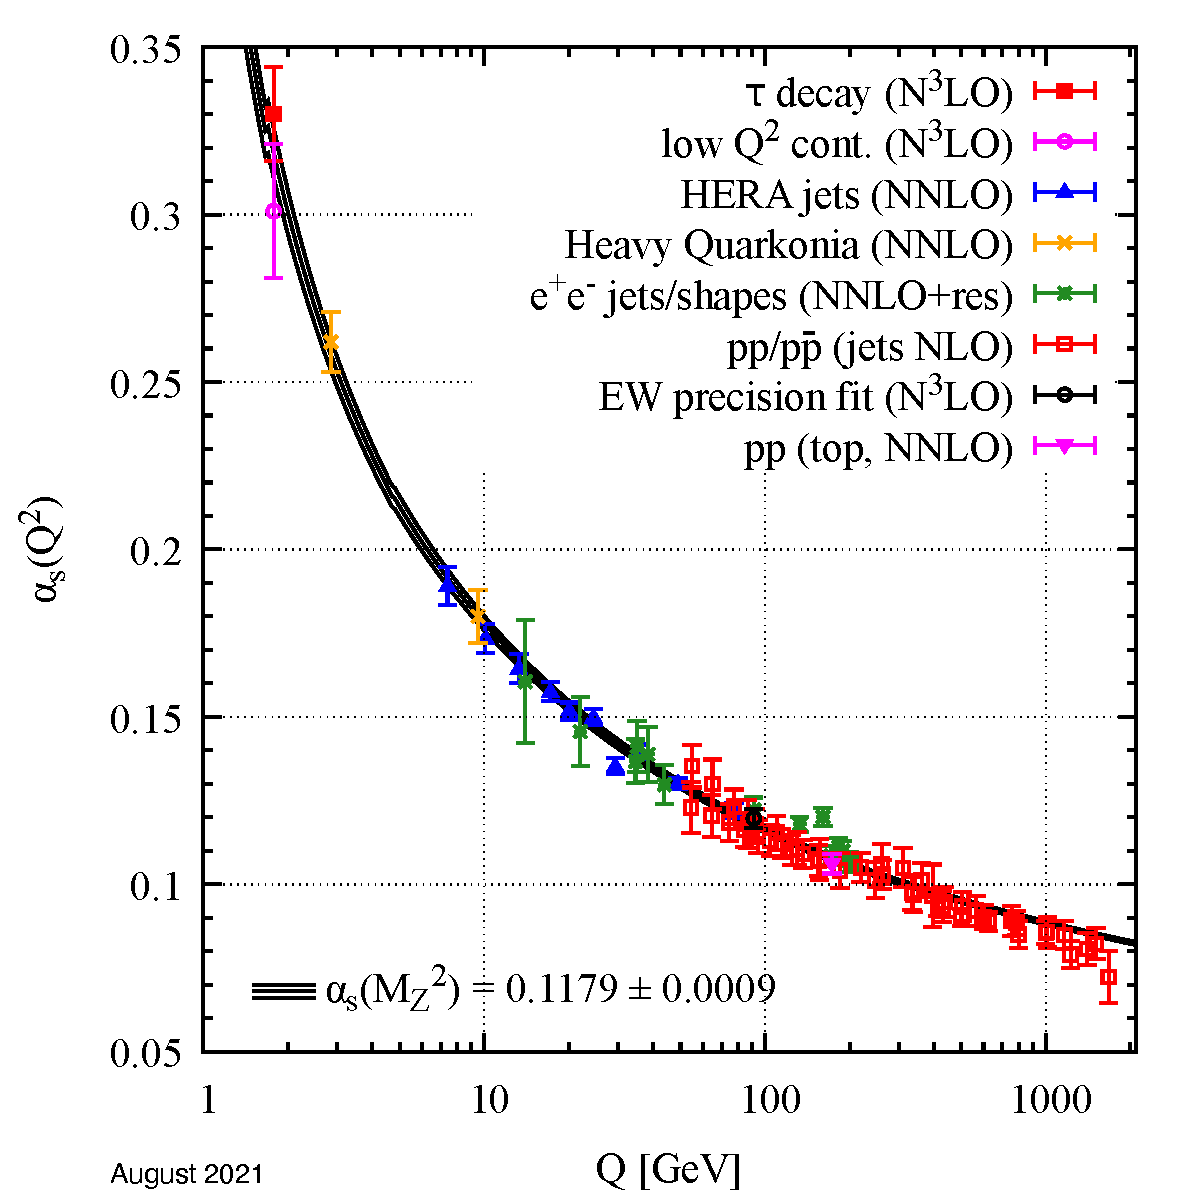
\includegraphics[width=0.8\textwidth]{Figs/Chapter2/alphas-v-Q-2021.pdf}
	\caption{Running of the coupling constant of the strong interaction, \alphaS, as a function of the energy \DIFdelbeginFL \DIFdelFL{tranfer }\DIFdelendFL \DIFaddbeginFL \DIFaddFL{transfer }\DIFaddendFL $Q$. The markers represent measurements based on perturbative calculation (the order of the perturbation development is indicated in parenthesis), the solid line corresponds to analytical prediction. Figure taken from \DIFdelbeginFL \DIFdelFL{\mbox{%DIFAUXCMD
\cite{particledatagroup2022}}\hspace{0pt}%DIFAUXCMD
}\DIFdelendFL \DIFaddbeginFL \DIFaddFL{\mbox{%DIFAUXCMD
\cite{particledatagroupReviewParticlePhysics2022}}\hspace{0pt}%DIFAUXCMD
}\DIFaddendFL .}
	\label{fig:RunningAlphaS}
\end{figure}

\Fig\ref{fig:RunningAlphaS} shows the running of the coupling constant \alphaS of QCD as a function of the energy transfer $Q$. The strength of the interaction varies considerably, such that two regimes can be discerned: one at large $Q$ (or small distance) when the strong interaction is "weak" (\alphaS small), the other at small $Q$ (or large distance) when the coupling constant gets "strong" (\alphaS large). Usually, these two regimes are delimited by defining an energy scale, denoted as \LambdaQCD, at which $\alphaS \sim 1$. This corresponds to $\LambdaQCD \sim 200$ MeV\footnote{The definition of \LambdaQCD is convenient because it allows to classify quarks as a function of their mass hierarchy with respect to \LambdaQCD: $u$, $d$ and $s$ quarks belongs to the light-flavour sector (\DIFdelbegin \DIFdel{$\LambdaQCD \gg m_{s}, m_{u}, m_{d}$}\DIFdelend \DIFaddbegin \DIFadd{$\LambdaQCD \ll m_{s}, m_{u}, m_{d}$}\DIFaddend ), the others are heavy-flavour quarks ($m_{t}, m_{b}, m_{c} \gg \LambdaQCD$).}. Far above this value, the contribution of high-order diagrams decreases with their order such that most of them can be neglected, and QCD predictions can be calculated easily -- or in the some cases, it simply renders the calculations possible -- using perturbation theory. In this case, we talk about perturbative QCD (pQCD).

As the energy transfer decreases, the coupling constant increases and perturbative calculations starts to diverge until the point where it becomes infinite, at \LambdaQCD. At this value or below, QCD is dominated by the contributions from high-order diagrams and can not be treated perturbatively anymore. The only way out is to perform analytical calculations, which is not possible due to the complexity of QCD. A more viable option is to resort to numerical calculations. A well-established technique is called \textit{lattice QCD}, where to each (space-time) point of the lattice/grid corresponds a spinor field representing the quarks possibly connected (or not) by links describing the gluon vector field. Although it provides some insights on non-perturbative physics aspects of QCD, it is extremely demanding in terms of computational power and time -- these two factors being strongly dependent on the lattice size.\\

A phenomenological approach of QCD, supported by lattice calculations, can also be followed by considering that the interaction potential between two quarks separated by a distance $r$ is approximated by\footnote{The expression of the potential is experimentally motivated by the ordering in the spectra of the charmonium ($c\bar{c}$) and bottomium ($b\bar{b}$) bound states \cite{thomsonModernParticlePhysics2013} \cite{martinParticlePhysics2017}.}
\begin{equation}
V(r) \approx - \frac{\alpha_{s}(r)}{r} + \kappa r,
\label{eq:QCDPotential}
\end{equation}
where the constant $\kappa$ is typically about 1 GeV/fm \cite{martinParticlePhysics2017}. The alert reader recognises the first term as the Coulombian-potential, similar to the one in QED; the second term corresponds to an elastic spring-type force. As illustrated in \fig\ref{fig:QCDPotential}, they describe two specific behaviours of the QCD interaction potential.

\begin{figure}[t]
	\centering
	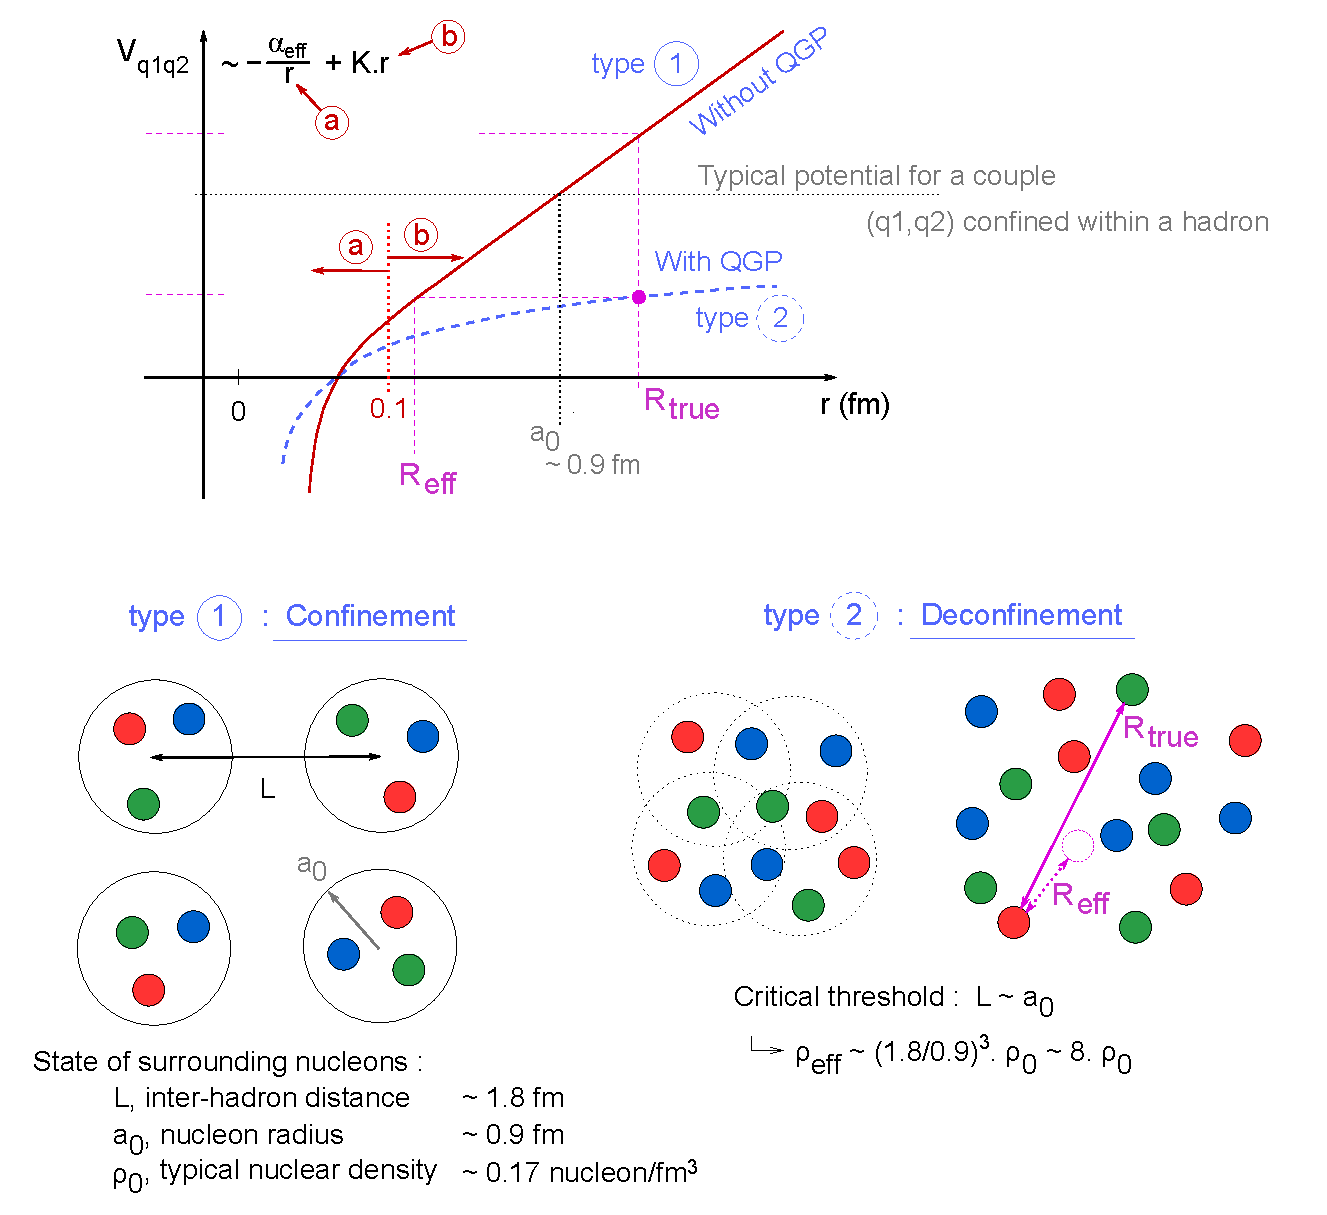
\includegraphics[width=0.9\textwidth]{Figs/Chapter2/GraphePotentiel.eps}
	\caption{QCD interaction potential between two coloured-objects (quark-quark or quark-antiquark) as a function of their separation $r$. Figure taken from \cite{maireProductionBaryonsMultietranges2011}.}
	\label{fig:QCDPotential}
\end{figure}

At small distance ($r \leq 0.1 \fm$), the Coulomb-type term dominates, the interaction potential diminishes asymptotically as the distance decreases; it is not divergent though, as \alphaS also varies. The quarks interacts less and less, and becomes quasi-free. This phenomenon, known as \textit{asymptotic freedom}, has been discovered by David Gross, Frank Wilczek in 1973 \cite{grossUltravioletBehaviorNonAbelian1973} and Hugh David Politzer in 1974 \cite{davidpolitzerAsymptoticFreedomApproach1974}, and \DIFdelbegin \DIFdel{set }\DIFdelend \DIFaddbegin \DIFadd{sets }\DIFaddend the groundwork for the development of a quantum field theory of strong interaction, that is the QCD\footnote{In the early seventies, the common belief among the theoreticians was that quantum field theory fails to describe the strong interaction, and therefore it would be impossible to have a common mathematical framework for all the known forces (except gravity) \cite{s.glashowInteractionsJourneyMind1990}.}. Neither the electrostatic force between two charges nor the gravitational force between two masses exhibit this property; in these cases, the interaction gets weaker as the distance increases between the two objects.

Conversely, the second term takes the upper hand at $r \geq 1 \fm$, the force increases linearly with the distance between the two quarks, as if they were connected by an elastic or spring made of gluons. As the quarks are pulled away, the energy stored in the spring of gluons accumulates until it reaches the threshold to create a quark-antiquark pair\footnote{There is an alternative scenario: the energy stored in the spring of gluons continues to increase until it reaches the threshold to create not one but two quark-antiquark pairs. Obviously, this path \DIFaddbegin \DIFadd{-- which explains the production of one or several baryons from the vaccum -- }\DIFaddend demands more energy and thus is less probable to occur.}. This description is shown on \fig\ref{fig:QuarkFragmentation}. The spring tying together the initial $q_{i}\bar{q}_{i}$ pair ruptures and the accumulated energy is expended on producing a $q_{1}\bar{q}_{1}$ pair: the freshly created quark, $q_{1}$, binds with $\bar{q}_{i}$,  $\bar{q}_{1}$ with $q_{i}$. This process continues until all the $q\bar{q}$ pairs have a sufficiently low energy to combine into a hadron. Note that the initial quark-antiquark pair could be replaced by a pair of gluons and the process would still be the same. As a result, any colour-charged particle -- quark or gluon -- can not be found isolated; they must be confined in a colour-neutral object, such as meson and baryon\footnote{If there is (\DIFdelbegin \DIFdel{ordinarly}\DIFdelend \DIFaddbegin \DIFadd{ordinarily}\DIFaddend ...) no such thing as free parton, the same would be true for a colour-charged hadron. For this reason, baryons and mesons are colour-neutral structures.}. This phenomenon is refered as \textit{colour confinement}.


Interestingly enough, the quark confinement is \DIFdelbegin \DIFdel{comparable }\DIFdelend \DIFaddbegin \DIFadd{analogous }\DIFaddend to the behaviour of a magnet. The latter consists of a north and south poles. If one tries to isolate one of the poles, for example, by cutting the magnet in half, this would only yield into two small magnets. Like the quarks, no one has ever seen an isolated magnetic pole (magnetic monopole).

\begin{figure}[t]
\begin{center}
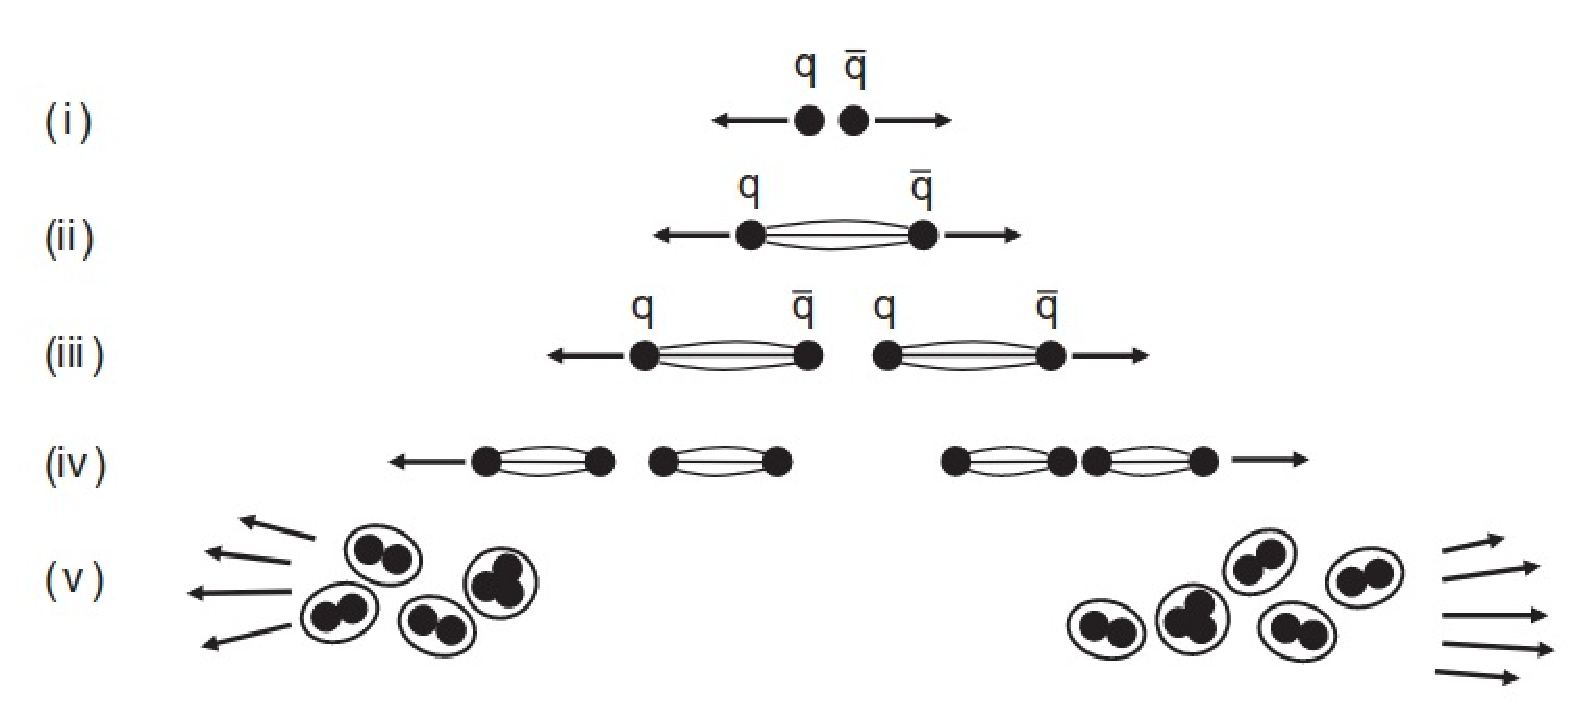
\includegraphics[width=0.9\textwidth]{Figs/Chapter2/Screenshot_20230220_214232.eps}
\end{center}
\caption{Schematic of the quark confinement: (i) the quark and antiquark are pulled away from each other;(ii) as they separated, the string of force tying together the pair stretches; (iii) the energy stored in the string now exceeds the necessary energy for creating a new quark-antiquark pair, the string will break and the two initial quarks will form smaller strings with the newly created pair;(iv) this process continues;(v) until all the quarks and antiquarks have a sufficiently low energy to form hadrons. Figure taken from \cite{thomsonModernParticlePhysics2013}.}
\label{fig:QuarkFragmentation}
\end{figure}

%On another note, hadrons can be classified as a function of their mass hierarchy of their quark constituent with respect to \LambdaQCD:
%\begin{itemize}
%\item[$\bullet$] Any hadron composed exclusively of up, down and strange valence quarks belongs to the \textit{light-flavour sector} ($\Lambda_{QCD} \gg m_{s}, m_{u}, m_{d}$)
%\item[$\bullet$] Any hadron containing, at least, one charm, bottom or top valence quark are members of the \textit{heavy-flavour sector} ($m_{t}, m_{b}, m_{c} \gg \Lambda_{QCD} $)
%\end{itemize}

\subsubsection{Chiral symmetry breaking}
\label{subsubsec:chiralsymmetrybreaking}

In \eq\ref{eq:LagrangianQCD}, the Lagrangian density of QCD was presented and \DIFdelbegin \DIFdel{splitted }\DIFdelend \DIFaddbegin \DIFadd{split }\DIFaddend into four different terms. The quark and gluon kinetic energy and the quark-gluon interaction terms preserve the chiral symmetry, meaning that they leave the chirality of the quarks unchanged. The mass term, though, mixes the left- and right-handed particles:
\begin{equation}
m_{q} \bar{\psi}_{q}^{i} \psi_{qi} = m_{q} \left( \bar{\psi}_{q}^{i, L} \psi_{qi}^{R} + \bar{\psi}_{q}^{i, R} \psi_{qi}^{L} \right).
\label{eq:LagrangianQCDMassTerm}
\end{equation}

The quark mass, $m_{q}$, controls whether the chiral symmetry is broken or preserved. For massless quarks, this term is null hence left- and right-handed particles do not interact together; they would live, somehow, in two separate worlds. Consequently, every hadron would have a twin, identical in every point apart from the handedness: one  is left-handed, the other right-handed. In practice, the quarks have a finite mass but, for the light-flavour ones, it is sufficiently small to consider the chiral symmetry as an approximate symmetry. Therefore, chiral partners are expected to have slightly different masses. However, this is clearly not the case of the $\rho$ ($m_{\rho} = 770 \mmass$) and $a_{1}$ ($m_{a_{1}} = 1260 \mmass$) mesons, meaning that the chiral symmetry is much more broken than expected \cite{kochAspectsChiralSymmetry1997}. 

To be exact, it is \textit{\DIFdelbegin \DIFdel{spontenously}\DIFdelend \DIFaddbegin \DIFadd{spontaneously}\DIFaddend } broken\footnote{Well, it is also \textit{explicitly} broken but we will pass on that detail.}. This concept is visualised in \fig\ref{fig:ChiralSymmetryBreaking}. Returning to the example in the note \ref{footnote:SpontaneousSymmetryBreaking}, the continuous transition of the ferromagnet is characterised by an order parameter: the magnetisation. When the temperature is so high that the thermal motions disrupt the alignement of all the magnetic dipoles, the potential is symmetric and the minimum is centred at zero magnetisation (left \DIFdelbegin \DIFdel{figure}\DIFdelend \DIFaddbegin \DIFadd{\fig}\DIFaddend ~\ref{fig:ChiralSymmetryBreaking}). As the temperature decreases and the magnet cools down, the symmetry of the potential is preserved but there are now two minima. The system (the ball) has to choose one, acquiring a non-zero magnetisation in the process, and hence breaking the symmetry (right \DIFdelbegin \DIFdel{figures}\DIFdelend \DIFaddbegin \DIFadd{\figs}\DIFaddend ~\ref{fig:ChiralSymmetryBreaking}). 

\begin{figure}[h]
	\centering
	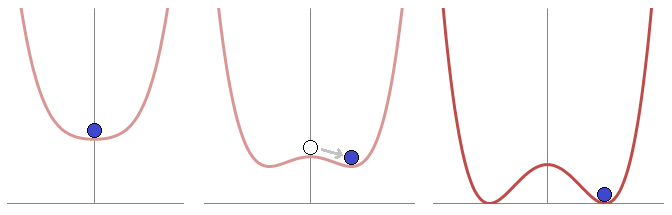
\includegraphics[width=\textwidth]{Figs/Chapter2/Spontaneous_symmetry_breaking_(explanatory_diagram).png}
	\caption{The left figure represents the shape of the potential at high energy, there is one minimum and it is centred on zero. Right figures: as the energy decreases and below a certain critical temperature, the ground state is no longer centred on zero but some distance away from it. Both ground states are equivalent, the system chooses one of them; this is a spontaneous symmetry breaking. The $x$-axis here represents the order parameter. Figure taken from \cite{ft2EnglishExplanatoryDiagram2012}.}
	\label{fig:ChiralSymmetryBreaking}
\end{figure}

The same process occurs for the chiral symmetry but, in this case, the order parameter is the \textit{chiral condensate}. This quantity, $< \psi_{q} \bar{\psi}_{q} > $ or $ < q \bar{q} >$, measures the coupling between left- and right-handed \DIFdelbegin \DIFdel{particle }\DIFdelend \DIFaddbegin \DIFadd{particles }\DIFaddend in vacuum. It was \DIFdelbegin \DIFdel{mentionned }\DIFdelend \DIFaddbegin \DIFadd{mentioned }\DIFaddend earlier that, in QFT, the vacuum is not empty but is composed of fleeting particle-antiparticle pairs that pop in and out. It could be that the Lagrangian density of QCD have an approximate chiral symmetry, but the vacuum does not. This means that particles with different handedness in the vacuum may (or not) interact together, depending the vacuum expectation value of the chiral condensate. If the $ < q \bar{q} >$ is null, the chiral symmetry is restored (left figure~\ref{fig:ChiralSymmetryBreaking}). Conversely, it is spontaneously violated when the chiral condensate is non-zero (right figures~\ref{fig:ChiralSymmetryBreaking}).

This symmetry was extensively studied by Yoichiro Nambu and Giovanni Jona-Lasinio in 1961 \cite{nambuDynamicalModelElementary1961}. In their model, the chiral condensate emerges from the passage of particles in the vacuum\footnote{In fact, the chiral condensate, and hence the spontaneous chiral symmetry breaking, is a consequence of the colour confinement \cite{peskinIntroductionQuantumField2018}.}; for that reason, the chiral symmetry breaking is qualified as \textit{dynamical}. Moreover, as the partons (inside a hadron) travel through the vacuum, they interact with the condensate and acquire an additionnal mass, the \textit{dynamical mass}\footnote{As opposed to the \textit{bare mass} stemming from the Higgs mechanism. It should be \DIFdelbegin \DIFdel{mentionned }\DIFdelend \DIFaddbegin \DIFadd{mentioned }\DIFaddend that nothing prevents the gluons to acquire also a dynamical mass. In this case, there would not be massless anymore.}. Predominant fraction of the hadron mass originates from this extra mass: for example, the proton mass sits $\sim 938$ \mmass and the bare mass of its quark constituents represents almost 10 \mmass, that is $\sim $ 1\% of proton mass.\\

On a side note, lattice QCD calculations predict that the chiral symmetry can be restored by heating or compressing matter. This is clear on \fig\ref{fig:ChiralSymmetryBreaking} where the chiral condensate vanishes as the temperature and/or density increases. In such conditions, the ordinary hadronic matter undergoes a phase transition, in which hadrons are only clothed by the bare mass of its constituents.

\begin{figure}[h]
\subfigure[]{
	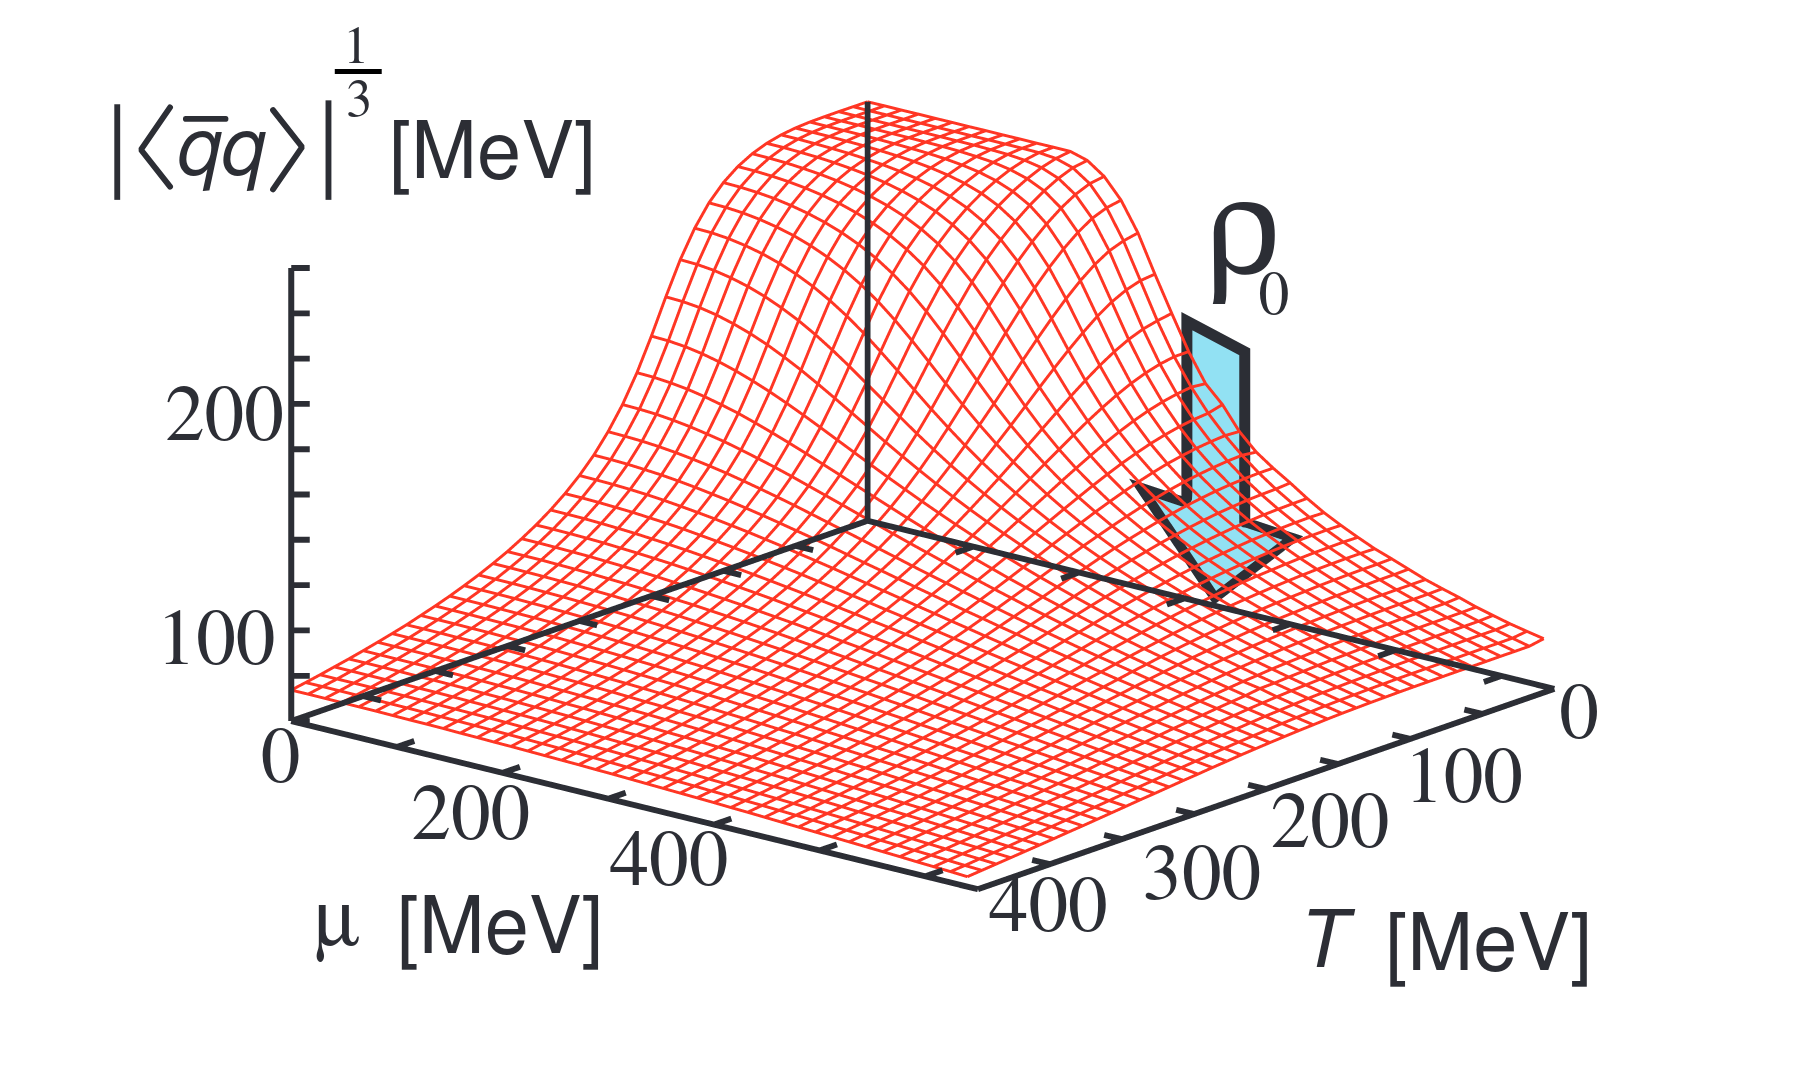
\includegraphics[width=0.50\textwidth]{Figs/Chapter2/ChiralCondensate.png}
}
\subfigure[]{
	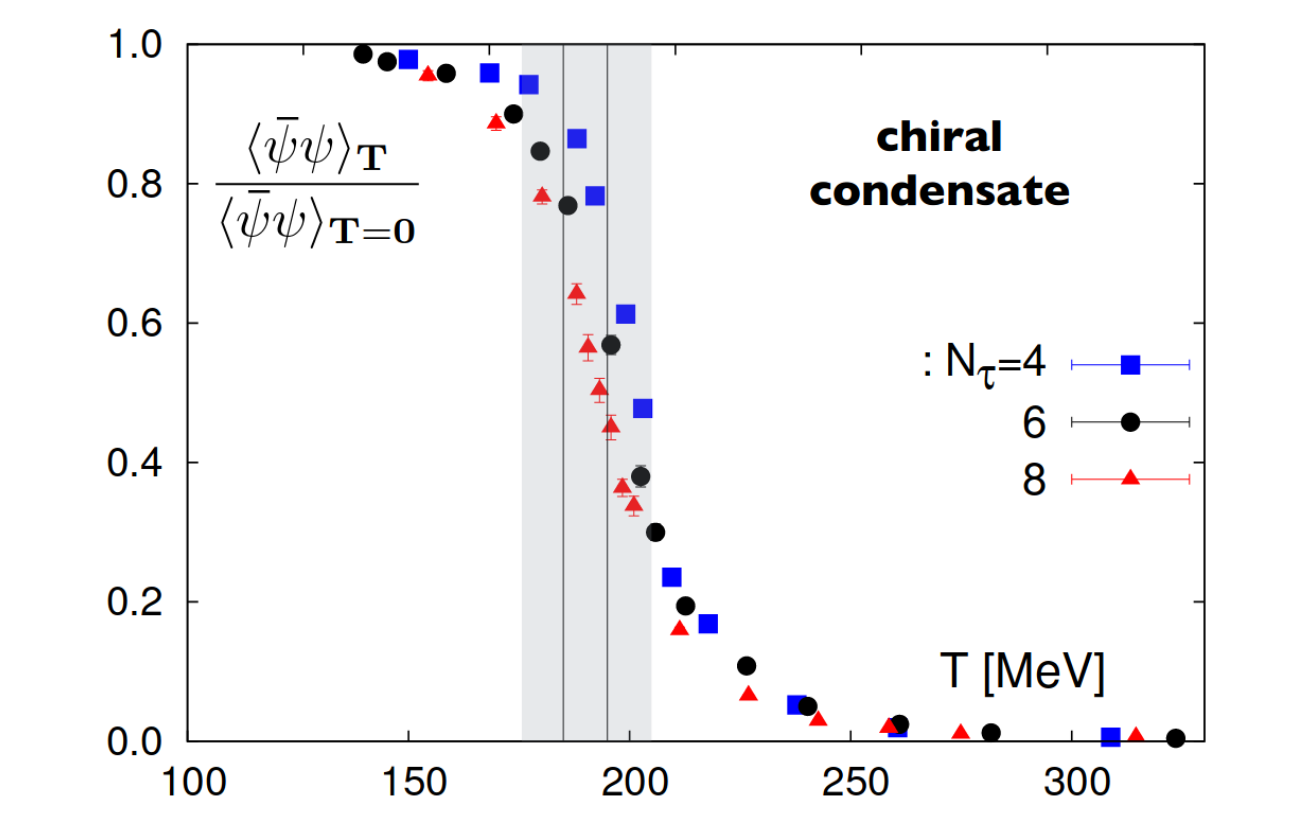
\includegraphics[width=0.50\textwidth]{Figs/Chapter2/ChiralCondensate2.png}
}
	\caption{Lattice QCD results on the evolution of the chiral condensate as a function of (a): the matter density (or the baryochemical potential $\mu$) and the temperature ($T$) \cite{muroyaLatticeQCDFinite2003}, (b): the temperature for different lattice points $N_{\tau}$ \cite{weiseChiralSymmetryStrongly2010}. The arrow on the left figure indicates the value of $\mu$ corresponding the ordinar nuclear density, $\rho_0$. The grey bands on the right figure indicate a range for the transition temperature.}
	\label{fig:ChiralSymmetryBreaking}
\end{figure}

\subsubsection{The QCD-phase diagram}
\label{subsubsec:QCDphasediagram}

In addition to the chiral phase transition, another one comes onto stage as the temperature increases. The \fig\ref{fig:QCDEnergyDensity} shows the predicted evolution of the pressure, energy density and entropy density for a hadron gas as a function of the temperature of the medium. The properties of the gas change rapidly when the temperature reaches $T_{c} = 154$ \mev, indicating the liberation of many degrees of freedom. In this case, these are the partons -- ordinarly confined within hadrons -- that now undergoes a \textit{deconfinement} transition and becomes quasi-free. 

I \DIFdelbegin \DIFdel{say }\DIFdelend \DIFaddbegin \DIFadd{write }\DIFaddend \textit{quasi}-free because even at $T \sim 400 $ \mev, the energy density does not reach the ideal gas limit. As a consequence, the quarks and gluons are still interacting but weakly. Due to this shared similarity with the plasmas, this new state of hadronic matter is dubbed \textit{quark-gluon plasma} (QGP). Note that, because the coupling between the partons decreases with the increasing momentum transfer and temperature (asymptotic freedom), the energy density will ultimately overlap with the ideal gas limit but at much larger temperature though. \\

\begin{figure}[h]
	\centering
	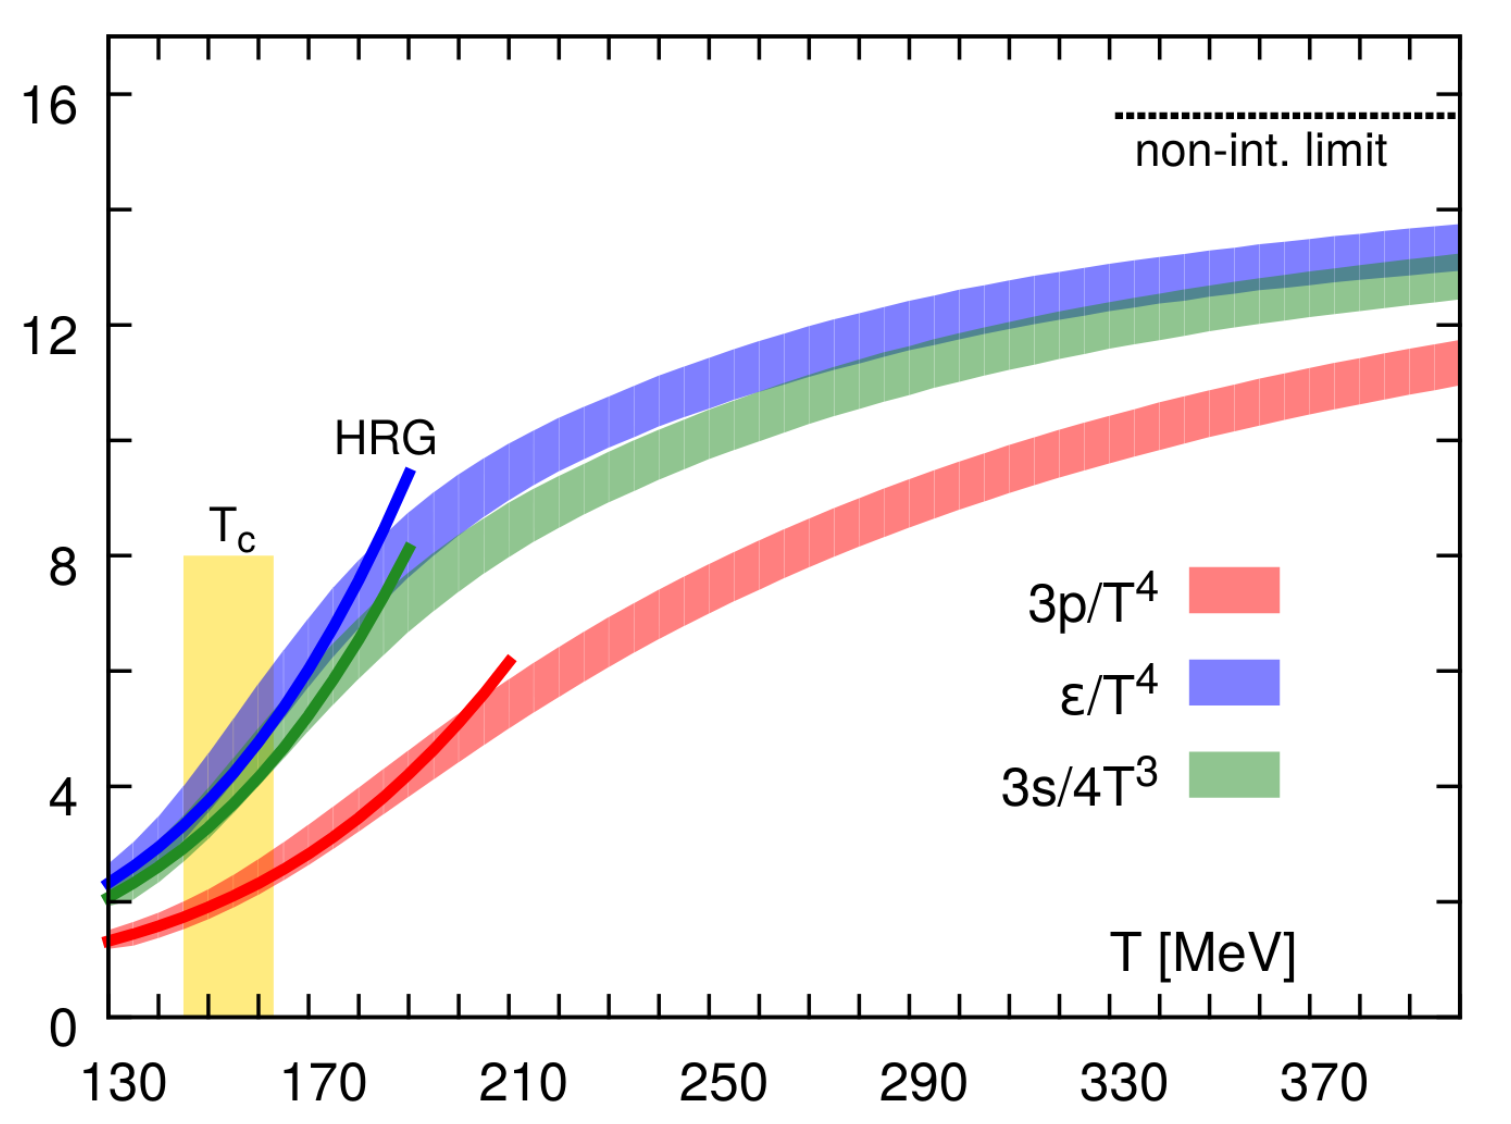
\includegraphics[width=0.7\textwidth]{Figs/Chapter2/Pressure_energy_entropy.png}
	\caption{Lattice QCD calculations of the pressure ($p$), energy density ($\epsilon$) and entropy density ($s$) normalised to the fourth (third, for the last quantity) power of temperature. The solid lines represent the prediction of the hadron resonance gas (HRG) model, the black dashed line indicates the energy density in the limit of an ideal gas. The transition temperature $T_{c}$ is equal to \DIFdelbeginFL \DIFdelFL{$154 \pm 9 \mev$}\DIFdelendFL \DIFaddbeginFL \DIFaddFL{$154 \pm 9$ }\mev\DIFaddendFL . It should be emphasised that these predictions have been obtained assuming a zero net baryon density. Figure taken from \cite{bazavovEquationStateFlavor2014}.}
	\label{fig:QCDEnergyDensity}
\end{figure}

The \fig\ref{fig:QCDPhaseDiagram} provides the full QCD phase diagram. As it can be seen, there are two general ways to form a quark-gluon plasma: either one increases the temperature, or one increases the net baryonic density by compressing hadronic matter. The above phase transition corresponds to the former: by heating up the system at (almost) zero net baryon density, ordinary nuclear matter transforms first into \DIFdelbegin \DIFdel{an }\DIFdelend \DIFaddbegin \DIFadd{a }\DIFaddend hadron gas and then undergoes a phase transition towards a QGP. This is what someone would see if he/she could rewind the videotape of the time-evolution of the Universe, from nowadays to a few \musec after the Big Bang. In the latter, the ordinary nuclear matter at relatively low temperature acquires, by compression, a larger and larger baryon density until the system transforms into a QGP. This state of matter is supposed to be present in the core of neutron stars\cite{annalaEvidenceQuarkmatterCores2019}, with potentially a colour superconductor behaviour \cite{alfordQCDFiniteBaryon1998}.

\begin{figure}[h]
	\centering
	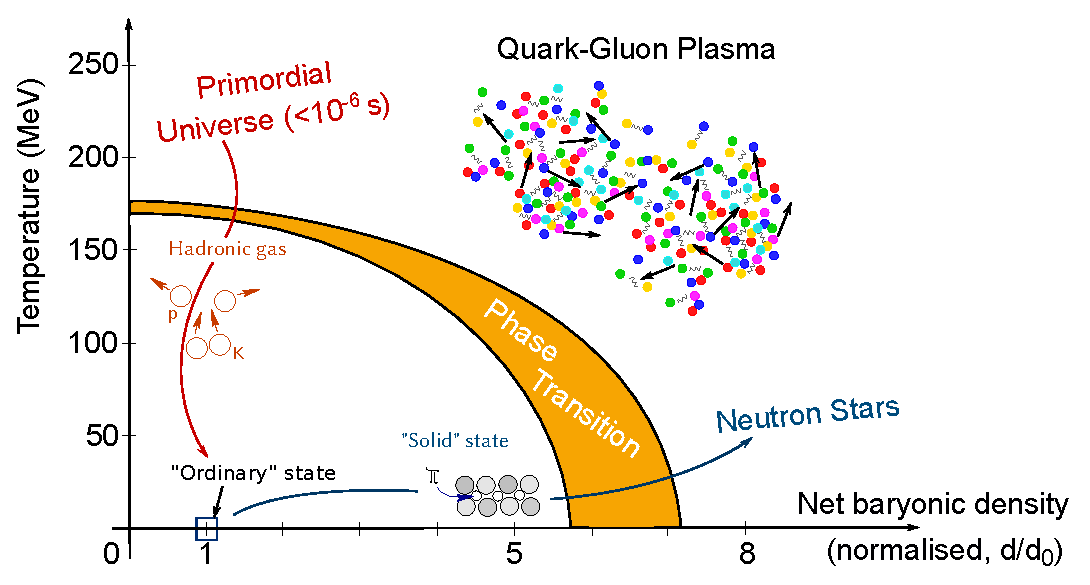
\includegraphics[width=\textwidth]{Figs/Chapter2/DiagrPhase.eps}
	\caption{Schematic representation of the QCD phase diagram as a function of the temperature and the net baryonic density. The latter is normalised to the net baryon density of ordinary nuclear matter. Figure taken from \cite{mairePhaseDiagramQCD2015}.}
	\label{fig:QCDPhaseDiagram}
\end{figure}

\DIFdelbegin \DIFdel{The }\DIFdelend \DIFaddbegin \DIFadd{There }\DIFaddend is a profund difference in the nature of the phase transition between the one \DIFdelbegin \DIFdel{at }\DIFdelend \DIFaddbegin \DIFadd{in }\DIFaddend the high-temperature \DIFaddbegin \DIFadd{region }\DIFaddend and the other with \DIFaddbegin \DIFadd{a }\DIFaddend high baryon density. Similarly to chiral transition on \fig\ref{fig:ChiralSymmetryBreaking}, the \fig\ref{fig:QCDEnergyDensity} shows a smooth evolution from one phase to another, indicating a second order --- or at least, a crossover --- phase transition \cite{philipsenQCDEquationState2013}. In contrast, the high baryon density driven evolution is expected to be more abrupt, more sharp as when ice melts to turn into water. This corresponds to a first order transition. It follows that there must be a critical point somewhere in the middle of the phase diagram, joining the first and second (or crossover) phase transitions \cite{stephanovQCDPhaseDiagram2005}. Its precise location is currently unknown, as no singularities have been observed yet.


\section{The Quark-Gluon Plasma}
\label{sec:QGP}

Each field of research has its pioneers and the study of the quark-gluon plasma is no exception. The first one was arguably Rolf Hagedorn, who approached the particle production making use of statistical physics. This endeavor led ultimately to the invention of the statistical bootstrap model (SBM) in 1964. At that time, a large number of massive resonances were observed, and this model provided a successful production mechanism for these particles\footnote{The statistical bootstrap model considers a gas of interacting hadrons, composed of all possible particles and their resonances, in a heat bath. If several light hadrons and/or resonances \DIFdelbegin \DIFdel{gets }\DIFdelend \DIFaddbegin \DIFadd{get }\DIFaddend compressed into a smaller volume, they could themselves be considered as a highly excited and massive resonance (also called fireball). Thus, the hadron gas rather corresponds to a gas of fireballs, that can also become a fireball in itself if compressed. This description provided an explanation for the mass spectrum of hadronic states.}. However, this description was conceived before the development of the quark model. When the quarks were finally considered as the elementary building blocks of hadrons, an extension of SBM was called for \cite{rafelskiMeltingHadronsBoiling2015a}.

The mutation of the statistical hadronisation model was achieved by the father of SBM and Johann Rafelski, between 1977 and 1980. This process led to a new paradigm. It was realised that, at a certain temperature, hadrons are melting to form a new phase composed of boiling quarks: the quark-gluon plasma. Although this concept was already intuited before by numerous physicists -- including Peter Carruthers in 1974 \cite{rafelskiMeltingHadronsBoiling2015} or George F. Chapline and Arthur K. Kerman in 1978 \cite{chaplinePossibilityMakingQuark1978} --, it was only approached qualitatively.

Nevertheless, Chapline and Kerman were the first ones to make the connection between the QGP and (relativistic) heavy-ion collisions. The same year, this point is addressed quantitatively by Siu A. Chin\cite{chinTransitionHotQuark1978a} and later refined in a paper by James D. Bjorken in 1983 \cite{bjorkenHighlyRelativisticNucleusnucleus1983}. In this renowned publication, Bjorken presents an analytical solution for one-dimensional relativistic hydrodynamics in heavy-ion collisions, as well as the space-time evolution of the QGP at mid-rapidity (\textit{Bjorken scenario}), laying down the foundations for the research programme at CERN.\\

Starting in 1986, a vast number of heavy ion experiments emerges at the CERN's Super Proton Synchrotron (SPS): WA85, NA36, NA35, Helios-2, NA38, WA80, and their future descendants \cite{satzSPSHeavyIon2004}. At first, $^{16}$O and $^{32}$S nuclei were accelerated at 200 \gev (per nucleon) until 1995, when the SPS switched to $^{208}$Pb beams with an energy per nucleon of 158 \gev. In a press conference held in February 2000, CERN reports to have \DIFdelbegin \DIFdel{"compelling evidence that a new state of matter has been created. The new state of matter found in heavy-ion collisions at the SPS features many of the characteristics of the theoretically predicted quark-gluon plasma" }\DIFdelend \DIFaddbegin \say{compelling evidence that a new state of matter has been created. The new state of matter found in heavy-ion collisions at the SPS features many of the characteristics of the theoretically predicted quark-gluon plasma} \DIFaddend \cite{NewStateMatter2023}. This announcement marks a turning point for QGP research: partonic matter is not a mere theoretical concept anymore; it becomes real, tangible and measurable. 

The Relativistic heavy-ion Collider (RHIC) at BNL enters in operation in the next few months, with its four experiments -- BRAHMS \cite{arseneQuarkGluonPlasma2005}, PHOBOS \cite{alPHOBOSPerspectiveDiscoveries2005}, PHENIX \cite{phenixcollaborationFormationDensePartonic2005}, STAR \cite{starcollaborationExperimentalTheoreticalChallenges2005} -- dedicated to observe and characterise the QGP under different observables. In April 2005, BNL holds a press conference in order to present the results of the RHIC experiments, and by doing \DIFdelbegin \DIFdel{, so}\DIFdelend \DIFaddbegin \DIFadd{so, }\DIFaddend confirms the existence of "a new type of nuclear matter" \cite{ludlamHUNTINGQUARKGLUON2005}.

Nowadays, the study of the QGP is mainly centred around two accelerators: the RHIC at BNL and, since 2009, the Large Hadron Collider (LHC) at CERN. Alike RHIC, the latter also has four experiments: ATLAS, CMS, LHCb and ALICE. Although, they all have a heavy-ion research programme, ALICE is specifically designed to analyse the QGP. Concretely, it pursues the exploration of the QCD phase diagram and the characterisation of this new state of matter initiated at the RHIC, but at much higher energies. For comparison, the LHC delivers Pb-Pb collisions at a centre-of-mass energy per nucleon \sqrtSnn = 2.76 and 5.02 \tev, and Xe-Xe collisions at \sqrtSnn = 5.44 \tev. This is, at least, \DIFdelbegin \DIFdel{20 }\DIFdelend \DIFaddbegin \DIFadd{twenty }\DIFaddend times more energetic than at the RHIC. The \DIFdelbegin \DIFdel{presentation of the }\DIFdelend LHC accelerator, as well as the ALICE collaboration, \DIFdelbegin \DIFdel{is the role of }\DIFdelend \DIFaddbegin \DIFadd{are presented in }\DIFaddend the next chapter, \chap\ref{chap:ALICE}. 


\subsection{The time evolution of a heavy-ion collision}
\label{subsec:BjorkenScenario}

We timidly started above to raise the question \DIFdelbegin \DIFdel{on }\DIFdelend \DIFaddbegin \DIFadd{of }\DIFaddend how a heavy-ion collision leads to the formation of the QGP? This point was addressed by Bjorken in his scenario of the same name. Although the current description turns out to be more complex than anticipated, the Bjorken scenario still provides the key steps of the QGP formation process. The following discussion is structured around the \DIFdelbegin \DIFdel{\fig}\DIFdelend \DIFaddbegin \DIFadd{\figs}\DIFaddend \ref{fig:PbPbSimu} and \ref{fig:QGPEvol}\\

A facility, such as the LHC or RHIC, accelerates heavy nuclei to ultra-relativistic speed. At the LHC energies, the Pb nuclei in each beam are accelerated to, at least, 1.38 \tev\footnote{The least energetic Pb-Pb collision available at the LHC being \sqrtSnn = 2.76 \tev, each beam carries 1.38 \tev per nucleon.}, which corresponds to a Lorentz factor $\gamma$ of about 1500. Consequently, as Bjorken argued \cite{bjorkenHighlyRelativisticNucleusnucleus1983}, even though the partons involved in the collision carry a tiny fraction of the incident beam energy, the nuclei are so extremely boosted that the space-time evolution of the system should be the same in all centre-of-mass frames near central rapidity, and thereby the particle yield should be flat as a function of rapidity, defining a central plateau structure for particle production. Moreover, at such energies, the nuclei are not stopped but rather continue to recede in opposite direction with respect to the collision point; this is the \textit{Bjorken regime} or \textit{transparency regime} and corresponds to net baryonic density close to zero\footnote{As opposed to the \textit{Landau regime} or \textit{stopping regime}, where the nuclei are completely stopped in frontal collisions. It occurs only for collisions at centre-of-mass energies up to a dozen of \gev \DIFaddbegin \DIFadd{per nucleon pair}\DIFaddend . These two regimes actually relates to the two different QGP phase transition: either by heating the system (Bjorken scenario) or compressing it (Landau scenario).}. Another implication is that, because of the length contraction, the nucleus looks like a highly-contracted pancake at mid-rapidity, as \DIFdelbegin \DIFdel{you can see on the }\DIFdelend \DIFaddbegin \DIFadd{can be seen on }\DIFaddend \fig\ref{fig:PbPbSimu}.\\

\begin{figure}[h]
	\centering
	\hspace*{-2cm}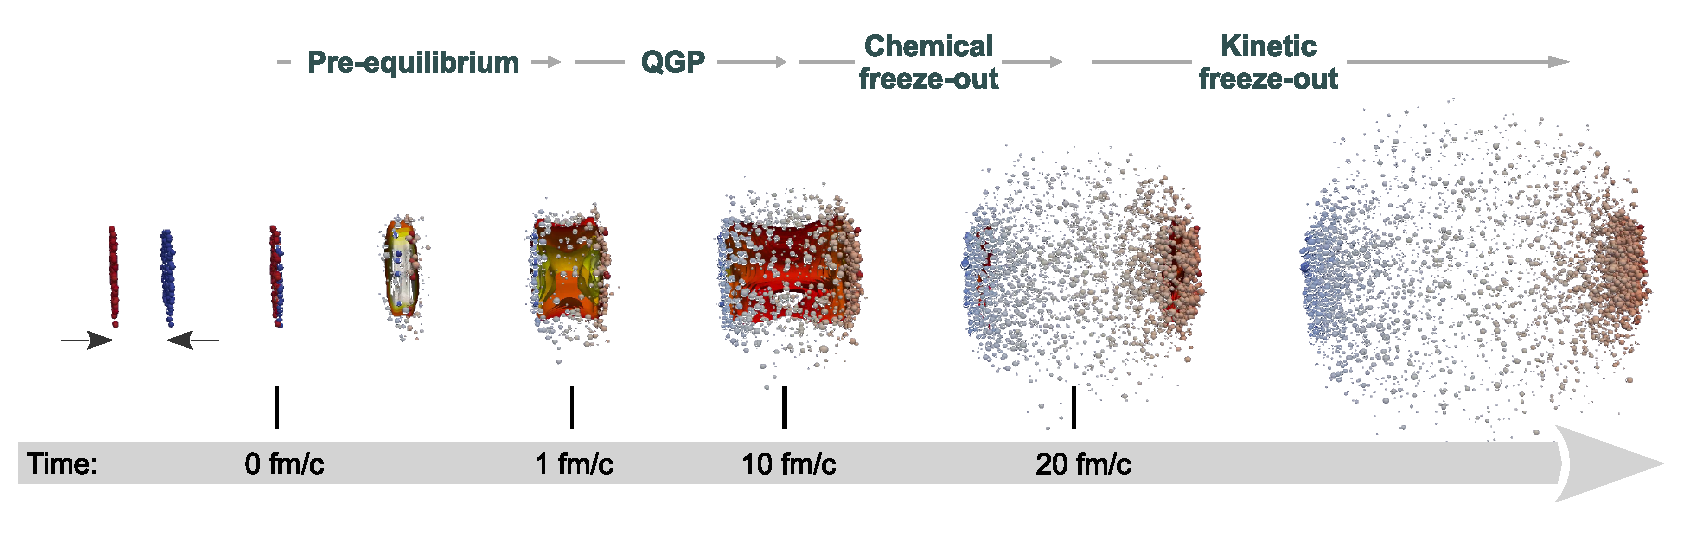
\includegraphics[width=1.35\textwidth]{Figs/Chapter2/PbPbCollision.eps}
	\caption{Simulation of the time evolution of a heavy-ion collision, rendered in seven pictures. Figure originally created by Hannah Petersen, taken from \cite{bernhardBayesianParameterEstimation2018} and modified by the present author.}
	\label{fig:PbPbSimu}
\end{figure}

\begin{figure}[h]
	\centering
	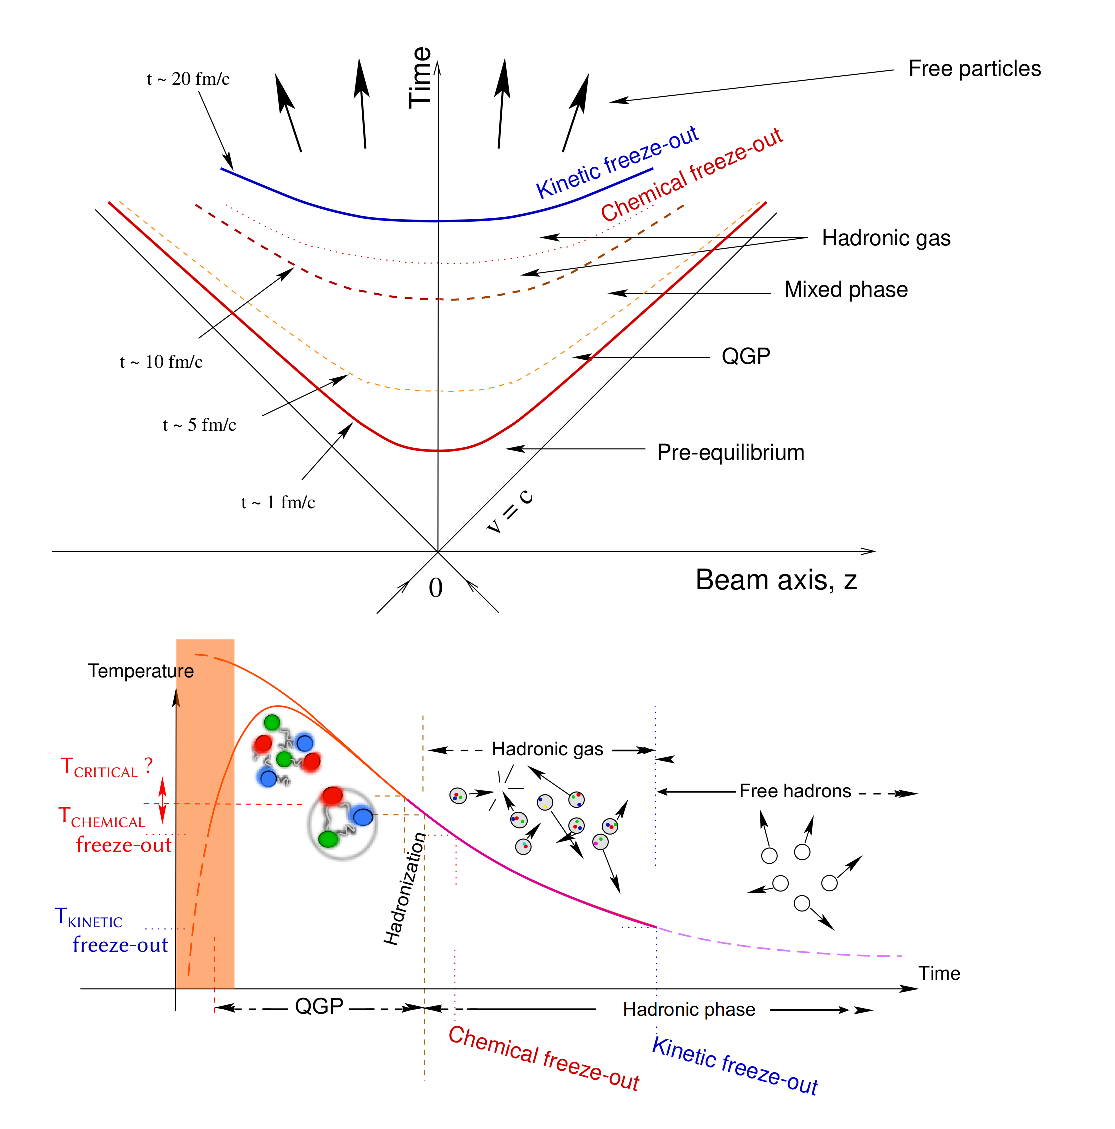
\includegraphics[width=\textwidth]{Figs/Chapter2/Schema-BjorkenScenario.eps}
	\caption{The two views of the Bjorken scenario for ultra-relativistic heavy-ion collisions. Top panel: space-time evolution. Bottom panel: temperature-time evolution. Figure taken from \cite{maireTwoViewsBjorken2011}.}
	\label{fig:QGPEvol}
\end{figure}

The two extremely boosted nuclei approach each other and collide head-on\footnote{Note that this is not \DIFdelbegin \DIFdel{necessarly }\DIFdelend \DIFaddbegin \DIFadd{necessarily }\DIFaddend the case, the two nuclei can be slightly shifted. The \textit{impact parameter} quantifies the offset usually in \fm, or alternatively in percentage. In the latter case, we talk about \textit{centrality}. Both parameters are accessible by making use of a \textit{Glauber model}, that provides a semi-classical picture of a nucleus-nucleus collision as a function of the average number of nucleons and nucleon participants in the collision.}. At the same time, the clock associated to the centre-of-mass frame starts to run and indicates 0 \fmC. 

The partons of each nuclei start interacting via either hard-processes -- that involve large momentum transfers and lead to the creation of high momentum partons or massive quarks such as the charm, bottom or even top quarks -- or soft-processes, characterised by small momentum transfer and representing most of the interactions in the initial stage of the collision. As the number of parton-parton interaction increases, the energy density of the system builds up enabling the creation of quarks and gluons out of the vacuum. Rapidly, a dense region of matter (dubbed "fireball") is formed, where partons are strongly coupled but not yet thermalised. This is the pre-equilibrium phase.

Here, the emphasis is on coloured particles, but other kind particles can be produced in the fireball, namely the leptons and photons. Because i) they carry no colour charge and ii) the typical interaction time of the weak ($\approx 10^{-10} \sec$) and electromagnetic forces ($\approx 10^{-16} \sec$) is too short compared to the timescale of a heavy-ion collision ($\approx 10^{-23} \sec$), they will simply escape the medium unaffected.

%\footnote{Here, the emphasis is on coloured particles, but other kind particles can materialise out of the vacuum, namely the leptons. Because i) they carry no colour charge and ii) the typical interaction time of the weak ($\approx 10^{-10} \sec$) and electromagnetic forces ($\approx 10^{-16} \sec$) is too short compared to the timescale of a heavy-ion collision ($\approx 10^{-23} \sec$), they will simply escape the collision environment.}


If the energy density is high enough (typically around 1 \gev/\fm$^{3}$), the initially produced matter undergoes, first, a phase transition towards the restoration of the chiral symmetry and, if possible, then towards the QGP. Due to multiple interaction between the medium constitutents, the energy gets distributed evenly among them leading the system to a thermal equilibrium around 1 \fmC ($\approx 10^{-23} \sec$) after the collision\footnote{Note that this is not a mandatory step for the QGP formation.}. 

Once the QGP is formed, it experiences two expansions. Driven by the non-uniform geometrical energy distribution in the initial stage of the collision, a pressure gradient appears in the QGP, which results in a radial expansion of the system. Furthermore, the boost of the two incident nuclei causes the plasma of quarks and gluons to inflate in the longitudinal directions. Since the energy deposited initially in the system is fixed and its spatial size keeps extending, the energy density decreases and inevitably, the fireball cools down.\\

At some point, most of the parts of the system goes below the critical temperature, the deconfined partons start to recombine into hadrons. The QGP evaporates into a gas of hadrons. Note, that because the chiral transition -- in this case, from a restored symmetry to a broken one -- occurs below $T_{c}$, the mesons and baryons formed during this hadronisation process only carry the bare mass of their constituents. At least, until the system further cools down and undergoes a phase transition towards a breaking of the chiral symmetry, as explained in the \Sec\ref{subsubsec:chiralsymmetrybreaking}.

The energy density within the hadron gas remains significant, sufficiently to allow for inelastic collisions. Consequently, the chemical composition in terms of particle species is in constant evolution. Around 10 \fmC, as the energy density decreases, inelastic interactions \DIFdelbegin \DIFdel{becomes }\DIFdelend \DIFaddbegin \DIFadd{become }\DIFaddend less and less frequent. They become impossible when the gas reaches the \textit{chemical freeze-out} temperature. The particle composition is now fixed but hadrons can \DIFdelbegin \DIFdel{only }\DIFdelend \DIFaddbegin \DIFadd{still }\DIFaddend interact elastically.\\

Although, the hadron content should be fixed, some resonances can still regenerate via pseudo-elastic scattering. This is, for example, the case of the \rmKstarZero that can be recreated through \rmPiPM-\Kminplus interaction. On the other hand, elastic scatterings modify the momentum of one of its decay products. In such a case, the measured yield would decrease.  

At 20 \fmC, the hadron gas fades into free hadrons. The momenta of the hadrons \DIFdelbegin \DIFdel{is }\DIFdelend \DIFaddbegin \DIFadd{are }\DIFaddend now fixed. This is the \textit{kinetic freeze-out}. These particles will fly towards the detectors and, for some of them, decay via weak or electromagnetic interactions. Either the particles originate directly from the collision or are decay products, once they have reached the detector, they will be detected and reconstructed, giving rise to an event such as the one displayed in the \fig\ref{fig:ALICEEventDisplay}.

\begin{figure}[h]
	\centering
	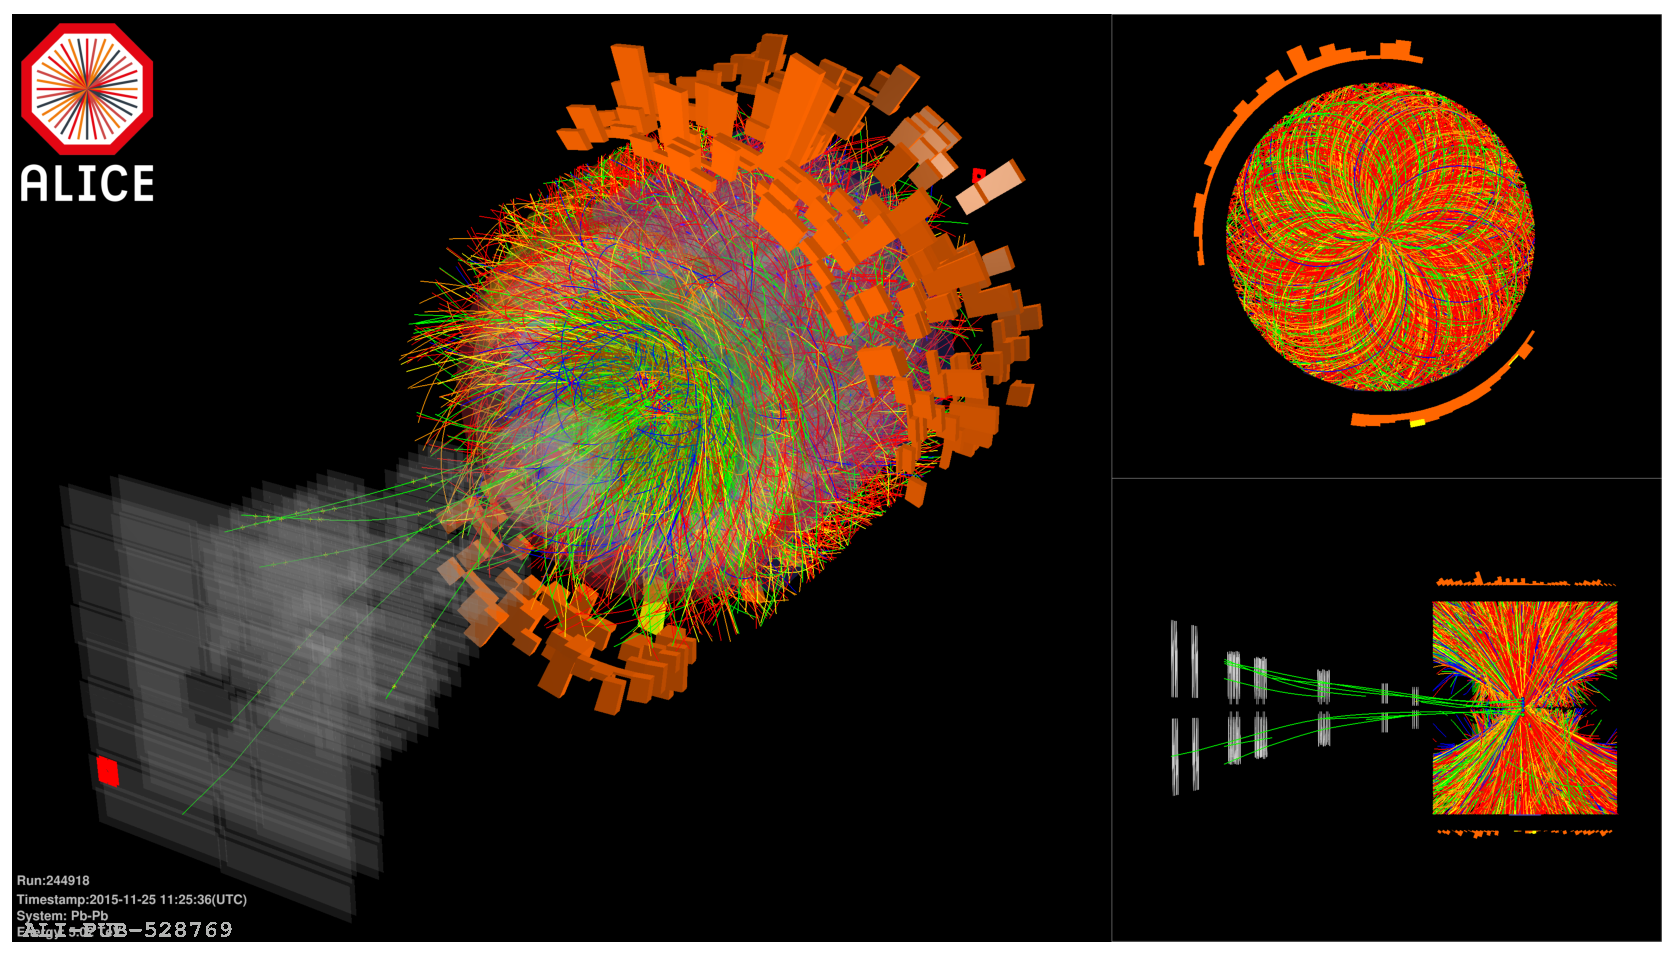
\includegraphics[width=\textwidth]{Figs/Chapter2/ALICE_EventDisplay.eps}
	\caption{Event display of the particles reconstructed with the ALICE detector and created in a Pb-Pb collision at \sqrtSnn = 5.02 \tev in 2015. Figure taken from \cite{alicecollaborationALICEExperimentJourney2022}.}
	\label{fig:ALICEEventDisplay}
\end{figure}

In total, the QGP only exists for about $10^{-22}\sec$, which is \DIFdelbegin \DIFdel{much shorter than }\DIFdelend \DIFaddbegin \DIFadd{currently impossible to reach for }\DIFaddend the most advanced readout electronics. The study of this state of matter relies on the signatures that are printed in the detectors after the collision. Theoretical models provide predictions of what the QGP footprints look like. Nowadays, it is widely admitted that the following signatures are marks of the QGP.

\begin{itemize}
\item[$\bullet$] \textbf{Collective flow:} The QGP being an almost perfect liquid \DIFaddbegin \DIFadd{of constituents with small mean free path}\DIFaddend , the pressure gradient created by the collision leads to a collective flow, \ie flow of partons, that can be described in the final state by ultra-relativistic hydrodynamic models.  This aspect is addressed, in particular, by performing measurements sensitive to the radial/isotropic and anisotropic flow. The former is characterised by a boost of the low-\pT produced hadrons to higher \pT --- the higher the mass, the higher the boost ---; the latter is studied through a Fourier series decomposition of the azimuthal \DIFdelbegin \DIFdel{dependence of the }\DIFdelend \DIFaddbegin \DIFadd{distribution of the emitted }\DIFaddend particle density. Moreover, the collective motion of partons can also be observed looking at long-range particle correlation.\\

\item[$\bullet$] \textbf{Direct photons:} Photo-production occurs over the entire duration of the collisions, but it is strongly increased when the system is hot. Therefore, a significant excess of \textit{direct}\footnote{The term \textit{direct} aims at designating only the photons originating from the different stage of the collisions (prompt), and not the ones from hadronic decays (non-prompt).} photons is observed in heavy-ion collisions, suggesting that a QGP has been formed there. Moreover, since they leave the medium unaffected, they carry informations on its properties. In particular, the low-\pT photons are essentially produced out of the plasma heat, hence they are designated as \textit{thermal photons}. Accounting for the blue-shift induced by radial expansion of the system (Doppler effect), the measurement of their yield provides an effective temperature of $304 \pm 41$ \mev in the most central Pb-Pb collisions \cite{alicecollaborationALICEExperimentJourney2022}.\\

\item[$\bullet$] \textbf{Jet quenching:} The high-\pT or massive partons are produced in the early stage of the collision. As they interact with \DIFdelbegin \DIFdel{the }\DIFdelend other soft partons of the QGP, a part of their energy is \DIFdelbegin \DIFdel{transfered }\DIFdelend \DIFaddbegin \DIFadd{transferred }\DIFaddend to the medium, resulting in energy loss effects. They are of two kinds: collisional, which consists in elastic scattering \textit{with} the medium constituents, and radiative that corresponds to an inelastic interaction and results in the emissions of \DIFdelbegin \DIFdel{gluon }\DIFdelend \DIFaddbegin \DIFadd{gluons }\DIFaddend \textit{within} the QGP. In the case of two jets, back-to-back, created close to the phase boundary, one will escape the fireball whereas the other will loose most of its energy in the medium. Thus, if one of the back-to-back jets is missing in the event, this would suggest the existence of a hot and dense medium, as observed in \cite{alicecollaborationSuppressionChargedParticle2011}\\

%However, the emission angle decreases with the number of emitted gluons, and the probability of radiating a gluon at a given angle depends on the parton mass. In particular for heavy quarks, there exists a cone region wherein there can be any gluon emission. This is called the \textit{dead cone effect}. Because of that, jets originating from a $c$ or $b$ quark will mainly loose energy \\
\item[$\bullet$] \textbf{Heavy quarkonia suppression:} The heavy quarks, such as charm or beauty, can fragment and hadronise to form a quarkonia ($c\bar{c}$ or $b\bar{b}$ mesons). Because of the low binding energy of these states, they will start to melt and dissolve within the medium. On the other hand, this suppression can be counter-balanced by a regeneration of the quarkonia state: at the chemical freeze-out, it is possible for a heavy quark to recombine with a heavy anti-quark. Therefore, the quarkonia production is compared to theoretical models, and so far, the results are consistent with the formation of a QGP.\\

\item[$\bullet$] \textbf{Hadron abundancy:} At \DIFdelbegin \DIFdel{the }\DIFdelend chemical freeze-out, the hadron gas is supposed to be in thermal and chemical equilibrium. The hadron composition in the hadron can therefore be addressed in a statistical approach using the grand canonical formalism. The \textit{statistical hadronisation model} (SHM) provides a prediction of the mesons and baryons abundancies, as a function of the gas volume and temperature, and the different chemical potentials ($\mu_{B}$ for the baryonic one, $\mu_{S}$ for the strangeness one,...). By fitting the measured yields of various hadron species with the SHM prediction, the chemical freeze-out temperature $T_{\textrm{ch}}$ and volume $V_{\textrm{ch}}$ can be estimated. The values $T_{\textrm{ch}} = 155 \pm 2 \ \mev$ and $V_{\textrm{ch}} = 5924 \pm 543 \ \fm^{3}$ are consistent with lattice QCD calculations. \\
\end{itemize}

About abundancy, the one of strange particles stands out of the other species. It is, in fact, one of the historical key signatures of the QGP and is called the \textit{strangeness enhancement}. 

\subsection{Strangeness enhancement}

The concept of strangeness enhancement, that consists in the abundant production of strange \DIFdelbegin \DIFdel{flavoured }\DIFdelend hadrons in heavy-ion collisions, starts to take shape in the mind of Johann Rafelski in 1980. The original argument is based on the assumption that, in a melted vacuum such as the one that settles in the QGP pre-equilibrium stage, the chiral symmetry restoration results in strange quarks carrying only their bare mass ($m_{s}$), \DIFdelbegin \DIFdel{which turns out to be }\DIFdelend \DIFaddbegin \DIFadd{that is }\DIFaddend at least two times lower than QGP temperature ($2 m_{s} < T_{\textrm{QGP}}$) . Thus, this opens the \DIFdelbegin \DIFdel{door for }\DIFdelend \DIFaddbegin \DIFadd{way to }\DIFaddend a chemical equilibration/saturation of strangeness. \DIFdelbegin \DIFdel{Moreover, when }\DIFdelend \DIFaddbegin \DIFadd{When }\DIFaddend the fireball cools down, the numerous $s$ and $\bar{s}$ tend to hadronise into \DIFaddbegin \DIFadd{strange }\DIFaddend baryons ($qqs$ or $\bar{q}\bar{q}\bar{s}$,...) rather than mesons ($\bar{q}s$ or $q\bar{s}$).

Back then, gluons were still hypothetical objects. Strangeness production was mainly considered in the annihilation process of light quark pairs $q\bar{q} \rightarrow s \bar{s}$ (\fig\ref{fig:StrangeYields}d). In 1981, J\'ozsef Zim\'anyi and Tam\'as B\'ir\'o estimated that, with this process, the chemical equilibrium of strangeness takes too much time to settle and is reached around eight times the natural lifespan of a QGP fireball. However, Zim\'anyi and B\'ir\'o assumed that there were no gluons and \DIFdelbegin \DIFdel{was }\DIFdelend \DIFaddbegin \DIFadd{were }\DIFaddend focused on the physical case of a hadron gas \cite{rafelskiStrangenessEnhancement2008}.

In parallel, it was realised that gluon fusion processes dominates the production rates. Together with Berndt \DIFdelbegin \DIFdel{Muller}\DIFdelend \DIFaddbegin \DIFadd{M\"{u}ller}\DIFaddend , Rafelski shows in 1982 that the chemical equilibration of strangeness is possible within the QGP lifespan thanks to the fusion of gluons created out of the vacuum heat  \cite{rafelskiStrangenessProductionQuarkGluon1982}. The different $gg \rightarrow s\bar{s}$ processes are depicted in \fig\ref{fig:StrangeYields}a,b,c.

%DIF > \begin{figure}[h]
%DIF > 	\centering
%DIF > 	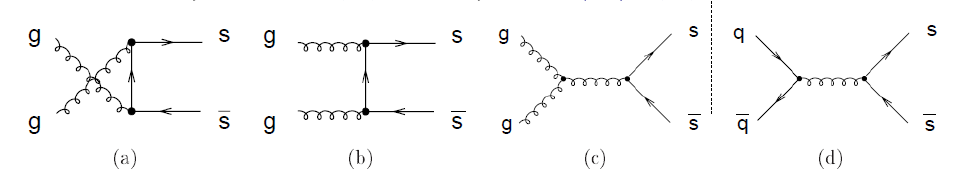
\includegraphics[width=1\textwidth]{Figs/Chapter2/Screenshot_20220620_004959.png}
%DIF > 	\caption{The lowest-order QCD diagrams for $s\bar{s}$ production. (a)(b)(c) the different gluon fusion processes $gg\rightarrow s\bar{s}$; (d) quark-antiquark annihilation process $q\bar{q} \rightarrow s\bar{s}$. Figure taken from \cite{maireProductionBaryonsMultietranges2011}.}
%DIF > 	\label{fig:StrangenessEnhancement}
%DIF > \end{figure}
\DIFaddbegin 

\DIFaddend \begin{figure}[h]
	\DIFaddbeginFL \begin{minipage}{0.33\textwidth}
		\subfigure[]{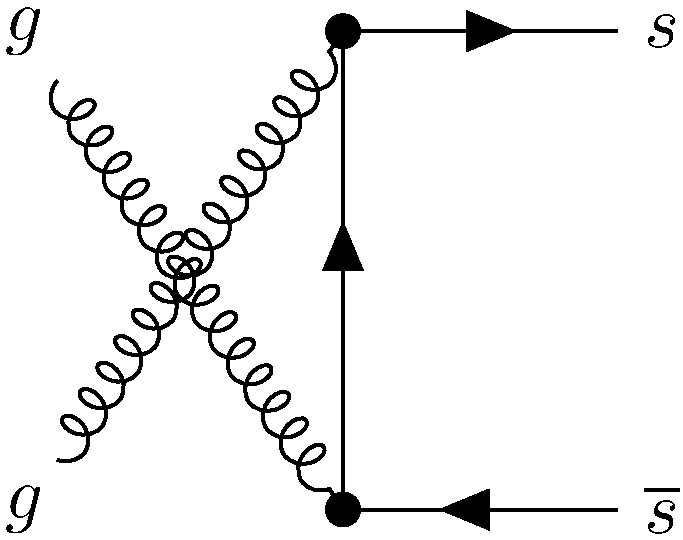
\includegraphics[width=0.75\textwidth]{Figs/Chapter2/g+g_crossed_to_s+sbar.pdf}}
	\end{minipage}%DIF > 
	\begin{minipage}{0.33\textwidth}
		\subfigure[]{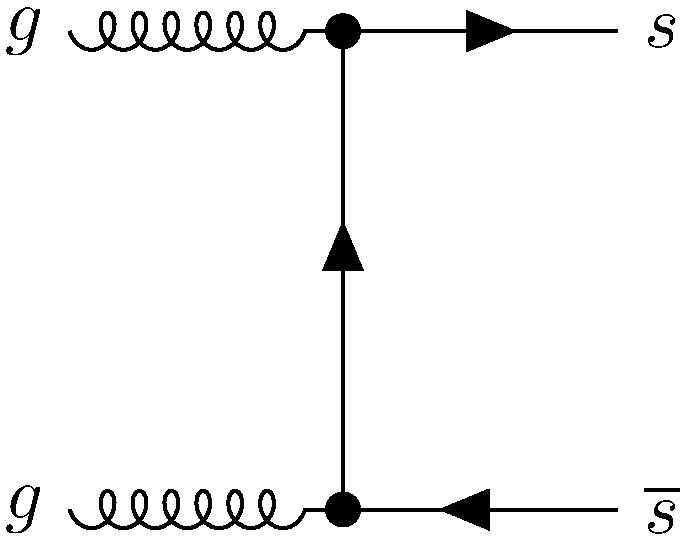
\includegraphics[width=0.75\textwidth]{Figs/Chapter2/g+g_square_to_s+sbar.pdf}}
	\end{minipage}%DIF > 
	\begin{minipage}{0.33\textwidth}
		\subfigure[]{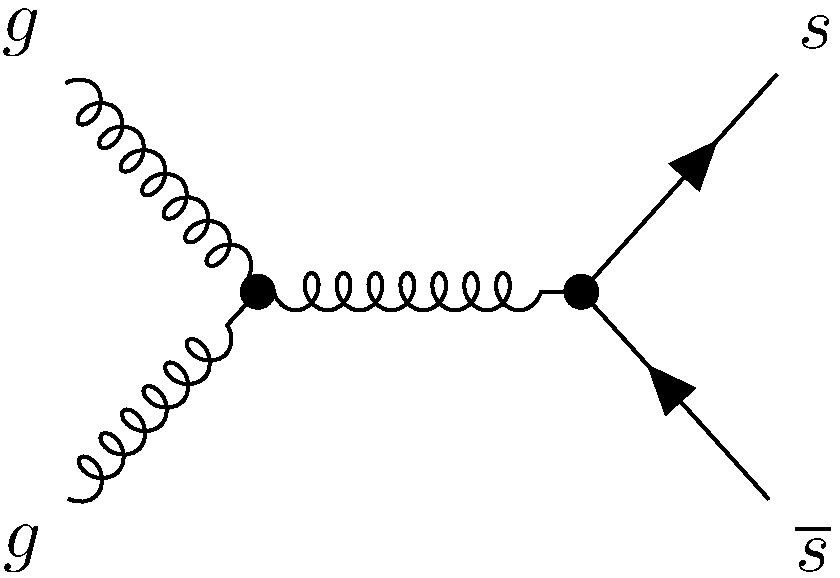
\includegraphics[width=0.90\textwidth]{Figs/Chapter2/g+g_to_gluon_to_s+sbar.pdf}}
	\end{minipage}\par\medskip
	\DIFaddendFL \centering
	\DIFdelbeginFL %DIFDELCMD < 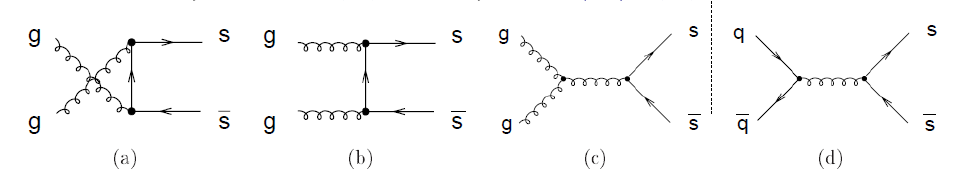
\includegraphics[width=1\textwidth]{Figs/Chapter2/Screenshot_20220620_004959.png}
%DIFDELCMD < 	%%%
\DIFdelendFL \DIFaddbeginFL \begin{minipage}{0.33\textwidth}
		\subfigure[]{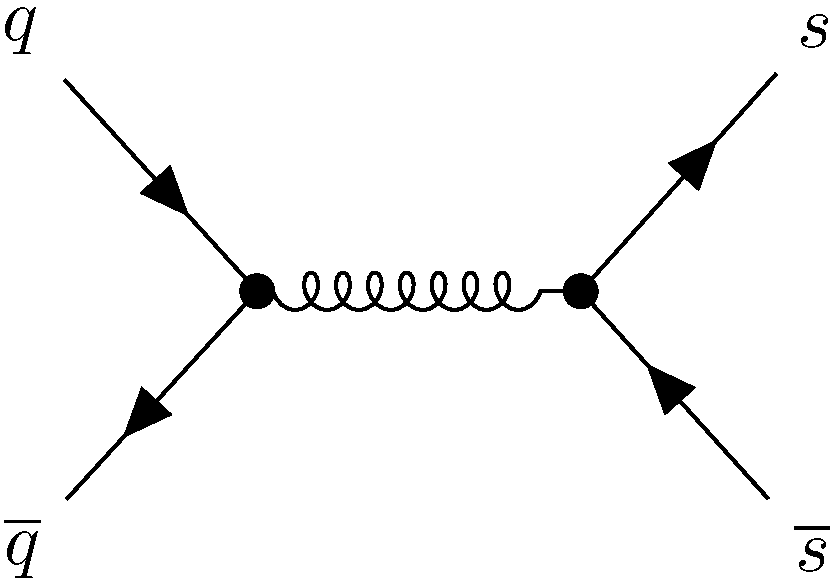
\includegraphics[width=0.90\textwidth]{Figs/Chapter2/q+qbar_to_gluon_to_s+sbar.pdf}}
	\end{minipage}%DIF > 
	\DIFaddendFL \caption{The lowest-order QCD diagrams for $s\bar{s}$ production. (a)(b)(c) the
	 different gluon fusion processes $gg\rightarrow s\bar{s}$; (d) quark-antiquark annihilation process $q\bar{q} \rightarrow s\bar{s}$. Figure taken from \cite{maireProductionBaryonsMultietranges2011}.}
	\label{fig:StrangenessEnhancement}
\end{figure}



In summary, the strangeness enhancement was proposed by Rafelski and \DIFdelbegin \DIFdel{Muller }\DIFdelend \DIFaddbegin \DIFadd{M\"{u}ller }\DIFaddend in 1982 as a signature of a deconfined quark-gluon matter. They demonstrated that:
\begin{itemize}
\item the QGP \DIFdelbegin \DIFdel{becomes }\DIFdelend \DIFaddbegin \DIFadd{begins to be }\DIFaddend saturated by strange quarks and anti-quarks when the temperature of the plasma reaches the 200 \mev \DIFdelbegin \DIFdel{around }\DIFdelend \DIFaddbegin \DIFadd{after about }\DIFaddend $2 \times 10^{-23} \sec$,
\item this saturation is possible because strange quarks can pop in out of the QGP heat ($2 m_{s} < T$) via gluon fusion processes (\fig\ref{fig:StrangenessEnhancement}). These processes are favoured because i) they are more energy/time efficient and ii) the high density of gluons created out of the vacuum,
\item at the hadronisation, the strangeness tends to be distributed on baryons rather than mesons. Consequently, this leads to an increased production of strange particles in the final state of the collision. In fact, the larger the strangeness content, the larger the enhancement of the hadron production.\\
\end{itemize}

Experimentally, the strangeness enhancement manifests itself through an increase of the \textit{relative} yields of strange hadrons in heavy-ion collisions. Now comes two difficulties: so far, only the strangeness enhancement from the formation of a QGP was considered, however a similar phenomenon could occur in a hadron gas\footnote{Strange hadrons could be formed via inelastic collisions between light mesons and baryons. Because of the large dynamical mass of hadrons, the production of strange particles should be suppressed. This reduction gets more pronunced as the hadron mass is high.}. The difference between these two \DIFdelbegin \DIFdel{increase }\DIFdelend \DIFaddbegin \DIFadd{increases }\DIFaddend in strange particle abundancies resides in the hierarchy between hadrons with different strangeness content \cite{maireProductionBaryonsMultietranges2011}:

\begin{align}
\rmOmega(sss)\ /\ \rmXi(dss) _{\textrm{QGP}} \quad &\approx \quad \rmXi(dss)\ /\ \rmLambda(uds) _{\textrm{QGP}}\\
\rmOmega(sss)\ /\ \rmXi(dss) _{\textrm{Hadron Gas}} \quad &\ll \quad \rmXi(dss)\ /\ \rmLambda(uds) _{\textrm{Hadron Gas}}
\end{align}

\begin{align}
\rmOmega(sss)\ /\ \rmXi(dss) _{\textrm{QGP}} \quad &> \quad \rmOmega(sss)\ /\ \rmXi(dss) _{\textrm{Hadron Gas}}\\
\rmXi(dss)\ /\ \rmLambda(uds) _{\textrm{QGP}} \quad &> \quad \rmXi(dss)\ /\ \rmLambda(uds) _{\textrm{Hadron Gas}}
\end{align}


Another issue arises from the definition of \textit{relative} yields. In other words, this comes down to asking what normalisation to use? There are different possibilities, depending on the physics target. Most of the time, the yields of strange hadrons in heavy-ion collisions \DIFdelbegin \DIFdel{is }\DIFdelend \DIFaddbegin \DIFadd{are }\DIFaddend compared to the \DIFdelbegin \DIFdel{one }\DIFdelend \DIFaddbegin \DIFadd{ones }\DIFaddend in pp collisions. This is relevant in order to discriminate the strangeness enhancement originating from the QGP (heavy-ion collisions) from the one occuring in a hadron gas (as in pp collisions, assuming that there are enough interactions between the different produced hadrons). Alternatively, one could also look at the "continuous" evolution of the yields as a function of the collision system. In such a case, the relative yields correspond to the ratio of production rate between the particle of interest and the lighest known hadron, namely the \rmPi. Finally, the focus can also be on the difference of yields between hadrons with the same strangeness content but different mass, typically the yields ratio between a resonant and a non-resonant hadronic state. This could provide some information on the influence of the hadronic phase.\\

\begin{figure}[h]
	\centering
	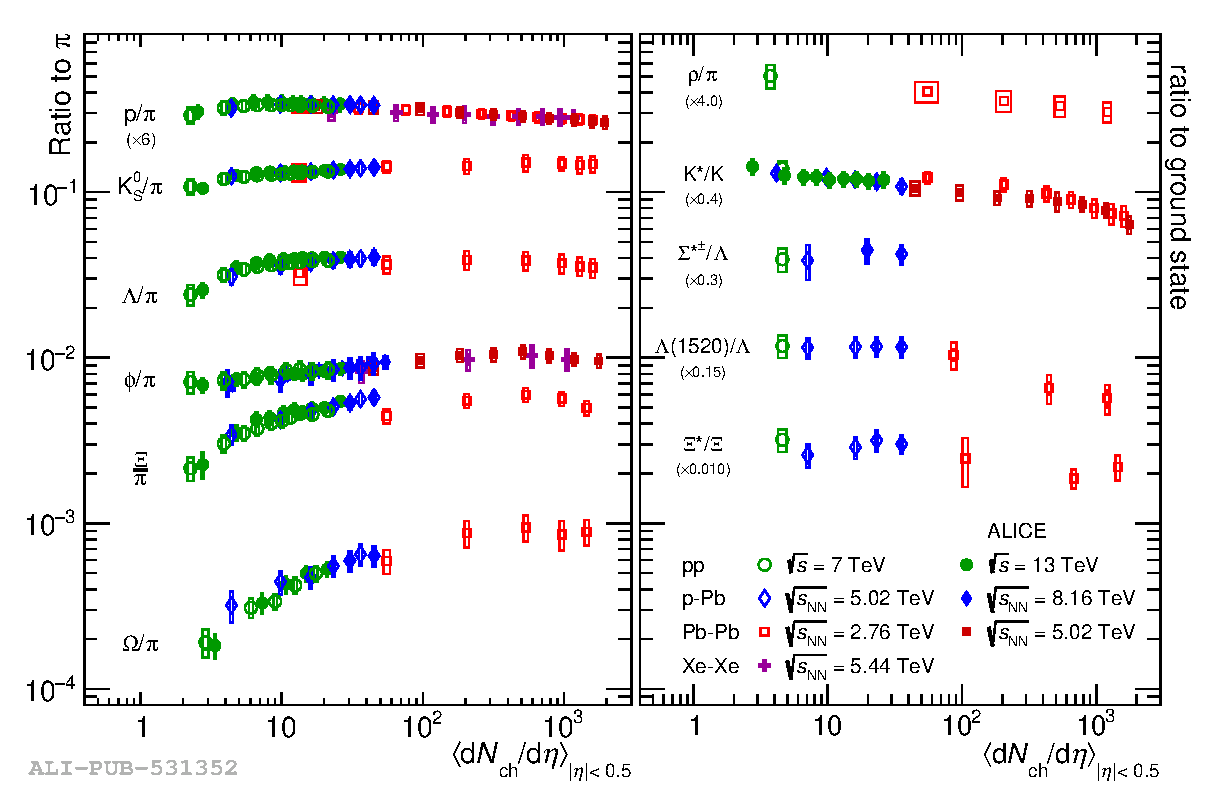
\includegraphics[width=1\textwidth]{Figs/Chapter2/fig3.2a.eps}
	\caption{(Left panel) Relative yields of strange hadrons with respect to the pions and (right panel) yield ratios between resonant and ground state hadrons as a function of the average charged particle multiplicities at midrapidity. Results from different collision \DIFdelbeginFL \DIFdelFL{system }\DIFdelendFL \DIFaddbeginFL \DIFaddFL{systems }\DIFaddendFL are \DIFdelbeginFL \DIFdelFL{present}\DIFdelendFL \DIFaddbeginFL \DIFaddFL{presented}\DIFaddendFL : pp at \sqrtS = 7 and 13 \tev; p-Pb at \sqrtSnn = 5.02 and 8.16 \tev; Pb-Pb at \sqrtSnn = 2.76 and 5.02 \tev; Xe-Xe at \sqrtSnn = 5.44 \tev. The left panel considers the following strange hadrons: \rmKzero ($\bar{d}s$), \rmLambda ($uds$), \rmPhi ($s\bar{s}$), \rmXi ($dss$) and \rmOmega ($sss$). The error bars corresponds to the statistical uncertainty, whereas the boxes show the total systematic uncertainty. Figure taken from \cite{alicecollaborationALICEExperimentJourney2022}.}
	\label{fig:StrangeYields}
\end{figure}

The \fig\ref{fig:StrangeYields} presents, on the left, the measurement of relative yields of strange hadrons with respect to the pions a function of the average charged multiplicity of the collision, and on the right, the yield ratios between resonant and non-resonant states are displayed. The lowest multiplicities correspond to pp collisions, and as it increases, we \DIFdelbegin \DIFdel{switch to }\DIFdelend \DIFaddbegin \DIFadd{move on towards }\DIFaddend more and more central heavy-ion collisions.

The left panel of \fig\ref{fig:StrangeYields} shows that the yield of strange hadrons increases in Pb-Pb and Xe-Xe collisions with respect to pp and p-Pb collisions, and the enhancement factor gets bigger with the strangeness content. This is compatible with the strangeness enhancement picture and confirms the existence of a deconfined quark-gluon matter. Notice that the ratios do not change with the centre-of-mass energy, suggesting that the initial stage of the collision does not play an important role in the strangeness enhancement \DIFaddbegin \DIFadd{(at least, at the LHC energies)}\DIFaddend .

On the right panel, the yield ratios between resonant and non-resonant hadronic states seems to decrease when going from elementary collision systems (pp and p-Pb) to the heavy-ion ones. This trend indicates that the temperature of the hadron gas after the QGP is sufficiently high to suppress the resonance yields by elastic rescattering of the decay products.

%\begin{figure}
%\unitlength = 1mm
%\centering
%\subfigure[]{
%	\begin{fmffile}{ggxss}
%	\begin{fmfgraph*}(40,25)
%	\fmfleft{i1,i2}
%	\fmfright{o1,o2}
%	\fmflabel{$g$}{i1}
%	\fmflabel{$g$}{i2}
%%	\fmflabel{$s$}{o1}
%%	\fmflabel{$\bar{s}$}{o2}
% 	\fmf{fermion}{o1,v1}
% 	\fmf{fermion,tension=0}{v1,v2}
% 	\fmf{fermion}{v2,o2}
% 	\fmffreeze
%	\fmf{gluon}{i1,v1}
%	\fmf{gluon,rubout}{i2,v2}
%%    \fmf{fermion}{i1,v1,v2,o1}
%%	\fmf{fermion}{o2,v4,v3,i2}
%%	\fmf{photon,tension=0}{v1,v3}
%%	\fmf{photon,tension=0}{v2,v4}
%	\end{fmfgraph*}
%	\end{fmffile}
%}
%\subfigure[]{
%	\begin{fmffile}{gghss}
%	\begin{fmfgraph*}(35,25)
%	\fmfleft{i1,i2}
%	\fmfright{o1}
%	\fmflabel{$g$}{i1}
%	\fmflabel{$g$}{i2}
%	\fmflabel{$g$}{o1}
%	\fmf{gluon}{i1,v1}
%	\fmf{gluon}{i2,v1}
%	\fmf{gluon}{v1,o1}
%	\fmfv{lab=$g_s$,lab.dist=0.15w}{v1}
%	\fmfdot{v1}
%	\end{fmfgraph*}
%	\end{fmffile}
%}
%\subfigure[]{
%	\begin{fmffile}{ggss}
%	\begin{fmfgraph*}(40,25)
%	\fmfleft{i1,i2}
%	\fmfright{o1,o2}
%	\fmflabel{$g$}{i1}
%	\fmflabel{$g$}{i2}
%	\fmflabel{$s$}{o1}
%	\fmflabel{$\bar{s}$}{o2}
%	\fmf{gluon}{i1,v1}
%	\fmf{gluon}{v1,i2}
%	\fmf{fermion}{v2,o1}
%	\fmf{fermion}{o2,v2}
%	\fmf{gluon}{v1,v2}
%	\fmfdot{v1}
%	\fmfdot{v2}
%	\end{fmfgraph*}
%	\end{fmffile}
%}
%\subfigure[]{
%	\begin{fmffile}{qqss}
%	\begin{fmfgraph*}(40,25)
%	\fmfleft{i1,i2}
%	\fmfright{o1,o2}
%	\fmflabel{$q$}{i1}
%	\fmflabel{$\bar{q}$}{i2}
%	\fmflabel{$s$}{o1}
%	\fmflabel{$\bar{s}$}{o2}
%	\fmf{fermion}{i1,v1}
%	\fmf{fermion}{v1,i2}
%	\fmf{fermion}{v2,o1}
%	\fmf{fermion}{o2,v2}
%	\fmf{gluon}{v1,v2}
%	\fmfdot{v1}
%	\fmfdot{v2}
%	\end{fmfgraph*}
%	\end{fmffile}
%}
%\caption{Using \texttt{test}}
%\end{figure}

\subsection{Comparison with elementary systems}
\label{subsec:ComparisonPP}

Throughout this section, it was suggested that the formation of the QGP is exclusive to heavy-ion collisions, and it is not expected in more elementary systems -- such as pp and p-Pb collisions -- \DIFdelbegin \DIFdel{due to }\DIFdelend \DIFaddbegin \DIFadd{because }\DIFaddend the size of the colliding system \DIFaddbegin \DIFadd{is }\DIFaddend \textit{a priori} too small. Looking more attentively at the \fig\ref{fig:StrangeYields}, one notices that relative yields of strange hadrons increases smoothly from low to high multiplicity pp and p-Pb collisions. In other words, this means that strangeness enhancement seems to be present as well in small systems.

In fact, the aforementionned QGP manifestations, the heavy quarkonia suppression \cite{adamCentralityDependence2S2016}, the strangeness enhancement \cite{alicecollaborationALICEExperimentJourney2022}, the collective flow \cite{schotterQCDLHC2022} have been observed in both heavy-ion collisions and small systems, suggesting the presence of a common collective behaviour. Some signatures are missing though; for example, there are so far no indication of jet quenching nor thermal photons in small systems. 

As a consequence, the classical picture of a heavy-ion collision, forming a hot and dense matter where quarks and gluons are deconfined, needs to be revised. At least, the elementary colliding systems can no longer be considered as a valid reference point\DIFaddbegin \DIFadd{, for sufficiently high energies such as the LHC ones}\DIFaddend . This point will be further addressed in more details in \chap\ref{chap:CorrelatedAnalysis}.



 \newpage  % Data sets
 \newpage \newpage
%//------ Section 02 -------------------------------------------------------------------------------------------------
\chapter{ALICE: A Large Ion Collider Experiment}
\label{chap:ALICE}
%//-----------------------------------------------------------------------//

As it was already mentionned before, ALICE (\textit{A Large Ion Collider Experiment})  aims at studying QCD bulk matter and, in particular, the quark-gluon plasma (QGP). It is situated in the CERN area, in the vicinity of Geneva, on the ring of the LHC (\textit{Large Hadron Collider}). Being the spearhead of the QGP studies at CERN, it has been designed in order to access to a large variety of observables \DIFdelbegin \DIFdel{, able to probe from the initial stage of the collision to the hadron gas phase, over a wide range of transverse momentum}\DIFdelend \DIFaddbegin \DIFadd{over a wide range of transverse momentum, thus offering the ability to study the evolution the heavy-ion collision from its initial stages to the hadronic phase}\DIFaddend .\\

The \DIFdelbegin \DIFdel{chapter begins with a brief presentation on CERN in \Sec\ref{sec:CERN} , putting forward the organisational and technical aspects , and most particularly the }\DIFdelend \DIFaddbegin \DIFadd{first section, \Sec\ref{sec:CERN} provides a brief introduction of the immediate surroundings of the ALICE collaboration, the CERN. Different aspects are mentioned, from the organisation to the main experiments on the LHC rings, through the CERN }\DIFaddend accelerator complex. \DIFdelbegin \DIFdel{Following the same structure, the \Sec\ref{sec:ALICECollaboration} provides a }\DIFdelend \DIFaddbegin \DIFadd{This brings to the }\DIFaddend description of the ALICE \DIFdelbegin \DIFdel{experiment}\DIFdelend \DIFaddbegin \DIFadd{in \Sec\ref{sec:ALICECollaboration}}\DIFaddend , from the \DIFdelbegin \DIFdel{collaboration to the detector before finishing with }\DIFdelend \DIFaddbegin \DIFadd{viewpoint of the collaboration and the experiment via the detector. The latter point allows to exhibit the strength of the ALICE detector, as well as presenting }\DIFaddend the event reconstruction \DIFaddbegin \DIFadd{procedure }\DIFaddend and the offline framework.


\section{The CERN}
\label{sec:CERN}

\subsection{The organisation}

Located the border between France and Switzerland, the CERN is like a tiny country with its own culture, its own language (essentially composed of acronyms). \DIFdelbegin \DIFdel{The \fig\ref{fig:CERNView} gives an aerial view of the CERN sites, with an insert on its headquarters in Meyrin (Switzerland, canton of Geneva). }\DIFdelend It is mostly known for its expertise on particle accelerators and detectors for high energy physics, but it is also the birthplace of some of our everyday devices -- such as the World Wide Web (1990), the touchscreen (1972) -- or less daily tools, like the Worldwide LHC computing grid (2005) and the multi-wire proportionnal chamber (1968). The \DIFaddbegin \DIFadd{\fig\ref{fig:CERNView} provides an aerial view of the CERN sites, with an insert on its headquarters in Meyrin (Switzerland, canton of Geneva). A location that has been decided from the very }\DIFaddend beginning of the organisation\DIFdelbegin \DIFdel{dates back to }\DIFdelend \DIFaddbegin \DIFadd{, back in }\DIFaddend the 1950s.\\

\begin{figure}[t]
	\centering
	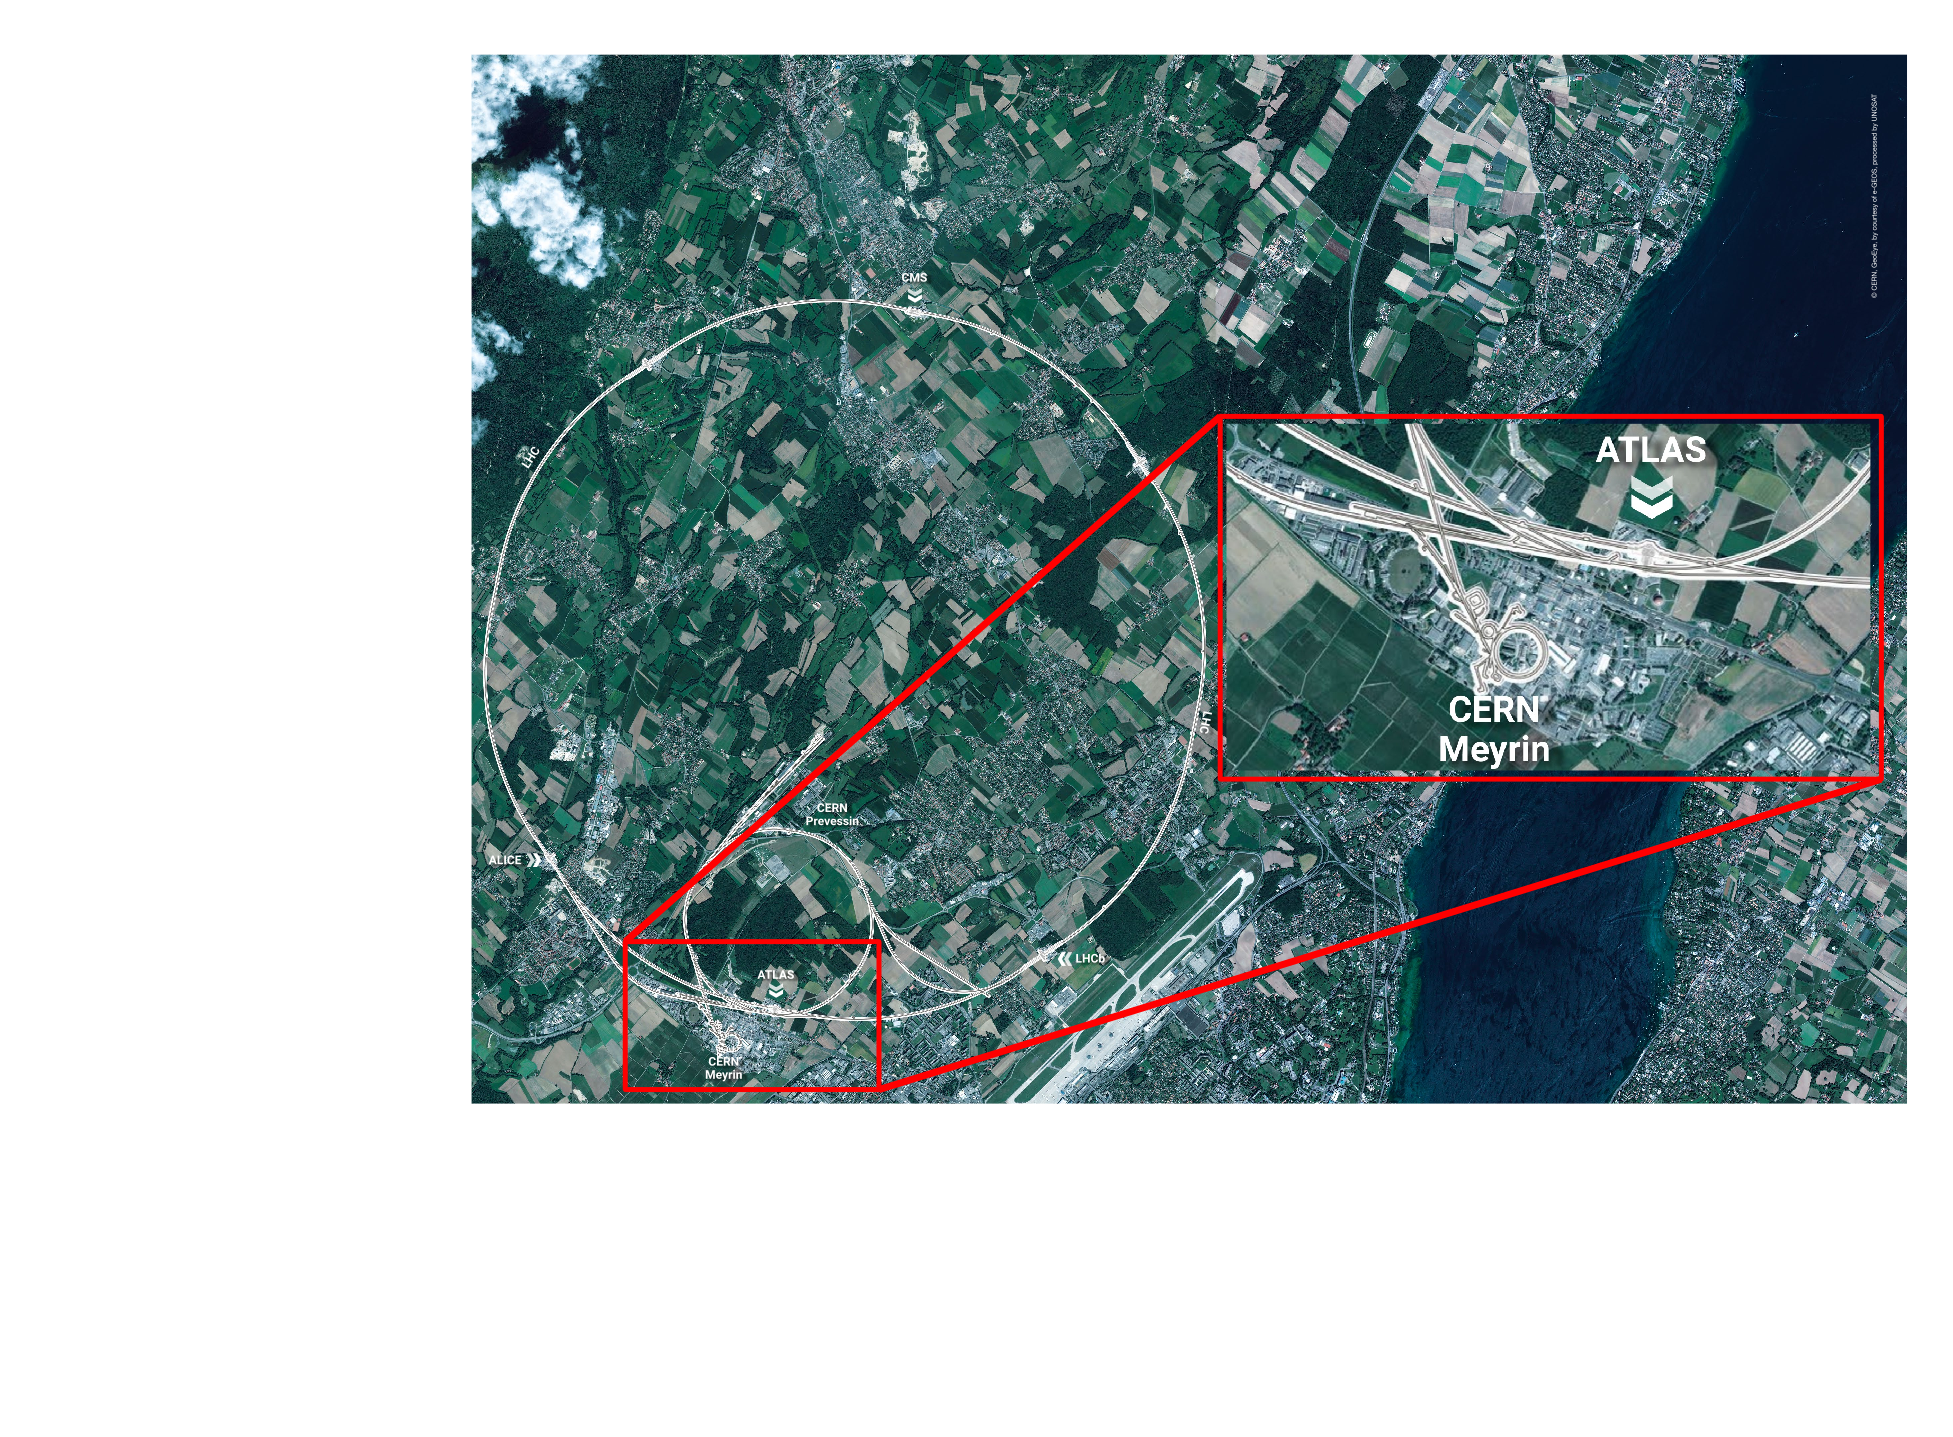
\includegraphics[width=1\textwidth]{Figs/Chapter3/CERN_Final.eps}
	\caption{Aerial view of the CERN accelerator complex (highlighted by the white curves), with an insert on the main site in Meyrin (Switzerland, canton of Geneva). Figure taken from \cite{PuzzleGrandCollisionneur} and modified by the present author.}
	\label{fig:CERNView}
\end{figure}

At the end of the Second World War, Europe lays in ruins, most of the research facilities \DIFdelbegin \DIFdel{have been destroyed , }\DIFdelend \DIFaddbegin \DIFadd{are destroyed and }\DIFaddend many physcists have left the continent to work on the other side of the Atlantic\DIFdelbegin \DIFdel{: }\DIFdelend \DIFaddbegin \DIFadd{. }\DIFaddend Europe is no longer at the forefront of scientific progress. A situation from which the old continent might never recover, as the european nations do not have the resources to rebuild the basic infrastucture. Nevertheless, things begin to change in 1949 when, at the European Cultural Conference, Louis de Broglie -- supported by Raoul Dautry, Pierre Auger, Lew Kowarsky, Edoardo Amaldi and Niels Bohr -- proposes to create an European laboratory in order to promote collaboration between Europe's nations, and share the costs.

The project gains momentum such that, in late 1951, the United Nations Educational, Scientific and Cultural Organization (UNESCO) -- pushed by the United States -- organises a dedicated meeting on that matter. Some countries shows their skepticism\DIFdelbegin \DIFdel{. This is not surprising}\DIFdelend : even though the infrastructure costs are mutualised, this kind of endeavor still demands an initial investement\DIFaddbegin \DIFadd{; a few years after the end of the war}\DIFaddend , many countries are \DIFaddbegin \DIFadd{still }\DIFaddend in a difficult financial position and are thus reluctant to participate. After two months of debate, the first resolution of the convention establishing the European Council for Nuclear Research (\DIFdelbegin \DIFdel{"Conseil Européen pour la Recherche Nucléaire" }\DIFdelend \DIFaddbegin \say{Conseil Européen pour la Recherche Nucléaire} \DIFaddend in French or CERN) is ratified in 1952 by the twelve founding member states: Belgium, Denmark, France, Germany, Greece, Italy, Netherlands, Norway, Sweden, Switzerland, United-Kingdom and Yugoslavia \cite{deroseParis1951Birth2008}.

Later that year, Geneva was chosen to host the laboratory. In 1953 the CERN convention is completed and signed by all the members. It defines, amongst others, the membership, the financial contributions, the decision protocols, its denomination\footnote{The CERN Convention was the opportunity to rename the CERN as the \DIFdelbegin \DIFdel{"Organisation Européenne pour la Recherche Nucléaire" }\DIFdelend \DIFaddbegin \say{Organisation Européenne pour la Recherche Nucléaire} \DIFaddend (or European Organisation for Nuclear Research in English), that would corresponds to the acronym OERN now. Because the initial abbreviation turns out to be more elegant, the \DIFaddbegin \DIFadd{name }\DIFaddend CERN remained.} and its missions. In particular, the CERN aims not only for technological developments and scientific \DIFdelbegin \DIFdel{research }\DIFdelend \DIFaddbegin \DIFadd{researches }\DIFaddend on high-energy physics but also for the \DIFdelbegin \DIFdel{"promotion of contacts between, and the interchange of, scientists, the dissemination of information }%DIFDELCMD < [%%%
\DIFdel{...}%DIFDELCMD < ]%%%
\DIFdel{", and "collaborating with and advising other research institutions" }\DIFdelend \DIFaddbegin \say{promotion of contacts between, and the interchange of, scientists, the dissemination of information [...]}\DIFadd{, and }\say{collaborating with and advising other research institutions} \DIFaddend \cite{cerncouncilConventionEstablishmentEuropean1953}.\\

Nowadays, the organisation includes 23 Member States and ten Associate Member States. There are also non-members States or institution with an Observer status, such as the United-States, Japan, European Union, UNESCO and \DIFdelbegin \DIFdel{formerly }\DIFdelend \DIFaddbegin \DIFadd{previously }\DIFaddend the Russian Federation. In 2017, the CERN counted more than 17 500 people, all over the world, working together towards a common goal, including more than 12 200 scientists \cite{cernOurPeople2023}. This makes it the largest scientific organisation in the World.

\subsection{The accelerator complex}
\label{subsec:AcceleratorComplex}

As stated in the Article II of the Convention, the construction and operation of particle accelerators stand as one of the CERN's purposes. In particular, the organisation must immediately develop a 600 \mev synchro-cyclotron and a 28 \gev proton synchrotron (PS). The former, built in 1957, corresponds to the first accelerator of CERN; the latter starts accelerating protons in 1959.

The next step up in beam energies arrives in 1976 with the first underground accelerator, the Super Proton Synchroton (SPS). It consists in two rings, of seven kilometers circumference each, delivering beams of 300 \gev of protons and antiprotons. At least, on the paper because it is one of the rare cases in particle physics, when the final product performs better than expected in the technical design reports. Thanks to technological advances during its construction, the SPS could reach beam energies up to 400 \gev, and gradually of 450 \gev after some upgrades.

In 1989, a 27-kilometre circular accelerator enters in operation, namely the Large Electron-Positron (LEP) collider. It was tuned such that the colliding energy sits on the resonance mass peak of the \rmZzero and \rmWplusminus bosons, but in the search of the Higgs boson, it was \DIFaddbegin \DIFadd{also }\DIFaddend operated with a centre-of-mass energy of 209 \gev on its last year, in 2000. This was -- and still is -- the largest electron-positron collider ever built.

As one World record calls for another, the LEP collider is decomissionned in order to be replaced in 2008\footnote{Technically, because of an incident on one of the dipole magnets, the accelerator undergoes some repairs that delay its operation by fourteen months.} by the Large Hadron Collider (LHC), the World's largest and most energetic particle collider. The accelerator is currently operational and should still be, at least, until 2038. Beyond this date, the CERN might start the construction of the Future Circular Collider, a particle accelerator with a circumference of 100 km\cite{FutureCircularCollider2023}\cite{benediktFutureCircularCollider2019}.\\

\DIFdelbegin %DIFDELCMD < \begin{table}[!h]
%DIFDELCMD <     %%%
\DIFdelendFL \DIFaddbeginFL \begin{table}[t]
    \DIFaddendFL \centering
    \begin{tabular}{p{5.5cm}@{\hspace{1cm}} p{2.25cm}@{\hspace{0.75cm}} p{2.25cm}@{\hspace{0.75cm}} p{2.25cm}@{}}
    \noalign{\smallskip}\hline\noalign{\smallskip}
    Collision type & pp & Pb-Pb & Xe-Xe \\
    Energy per beam & 6.5 \tev & 2.56 \tev & 2.72 \tev \\
    Luminosity ($cm^{-2} s^{-1}$) & $2.1 \times 10^{34}$ & $6.1 \times 10^{27}$  & $0.4 \times 10^{27}$ \\
    Velocity (in units of $c$) & 0.99999998 & 0.99715693 & 0.99898973 \\
    \noalign{\smallskip}\hline \noalign{\smallskip}
    Circumference & \multicolumn{3}{c}{26 659 m} \\
    Beam vacuum & \multicolumn{3}{c}{$10^{-13}$ atm} \\
    Number of RF cavities & \multicolumn{3}{c}{8 per beam} \\
    Number of magnets & \multicolumn{3}{c}{9593} \\
	Number of dipole magnets & \multicolumn{3}{c}{1232}\\
	Dipole operating temperature & \multicolumn{3}{c}{1.9 K (-271.3 C)}\\
	Current flowing in the dipole & \multicolumn{3}{c}{11 850 A}\\
	Magnetic field of the dipole & \multicolumn{3}{c}{8.33 T}\\
    \noalign{\smallskip}\hline\noalign{\smallskip}
    \end{tabular}
    \caption{A selection of design parameters for the LHC during the Run-2. Values taken from \cite{LHCGuide2017} and \cite{particledatagroupReviewParticlePhysics2022}.}\label{tab:LHCCharacteristics}
\end{table}

The LHC is the collider of (almost) all superlatives. To put it into perspectives, the \tab\ref{tab:LHCCharacteristics} lists some of its important characteristics. 

As in any accelerator, particles circulate in a vacuum tube in order to avoid collisions with gas molecules. The beam is subject to ultra-high vacuum, corresponding to a pressure of $10^{-13}$ atm, applied over the approximately 9 000 $m^{3}$ covered by the LHC. In comparison, this is like pumping down the nave of a cathedrale to a pressure level similar to the one \DIFdelbegin \DIFdel{on the Moon}\DIFdelend \DIFaddbegin \DIFadd{at the Moon's surface}\DIFaddend . 

\DIFdelbegin \DIFdel{The particle trajectoryis controlled by various magnets}\DIFdelend \DIFaddbegin \DIFadd{Various magnets control the particle trajectory}\DIFaddend : 1232 dipoles to bend the 6.5 \tev beams, 392 quadrupoles to squeeze and focus the beam down to the collision point, etc. If we hope to curve the particle's trajectory at the LHC energies, the dipoles must create an intense magnetic field of 8.33 T, demanding a current of 11 850 A. \DIFdelbegin \DIFdel{At }\DIFdelend \DIFaddbegin \DIFadd{For comparison: at }\DIFaddend ambient temperature, the dissipated heat would melt down the magnet. \DIFdelbegin \DIFdel{For that reason}\DIFdelend \DIFaddbegin \DIFadd{Hence}\DIFaddend , 90 tonnes of superfluid helium are injected into the magnets bringing their temperature down to 1.9 K (-271.3 C), that is even lower than the temperature of outer space (2.7 K). At this level, the dipoles become superconducting and can now \DIFdelbegin \DIFdel{bear }\DIFdelend \DIFaddbegin \DIFadd{endure }\DIFaddend the flow of currents to develop the necessary magnetic field. 

The particle acceleration is ensured by eight radiofrequency cavities (RF cavities)\footnote{It consists in a cavity filled with an electromagnetic field oscillating at a specific frequency (in the radio wave's domain, hence the name of the radiofrequency cavities), and shaped in such a way that resonance occurs.} per beam. Most often, they accelerate protons at 6.5 \tev, which corresponds to the typical kinetic energy of flying mosquito but distributed on the minuscule volume of a proton. At such energy, a proton travels at almost light-speed and makes 11 245 LHC turns per second. \DIFdelbegin \DIFdel{As a consequence }\DIFdelend \DIFaddbegin \DIFadd{Furthermore, because }\DIFaddend of the RF cavities, each beam is divided into 2808 bunches separated by 7.5 m (or 25 ns\footnote{This is the case for the LHC Run-2, but in the Run-1, the distance between two bunches was twice as big, that is 50 ns.}) and containing about $10^{11}$ protons. \\

\begin{figure}[t]
	\centering
	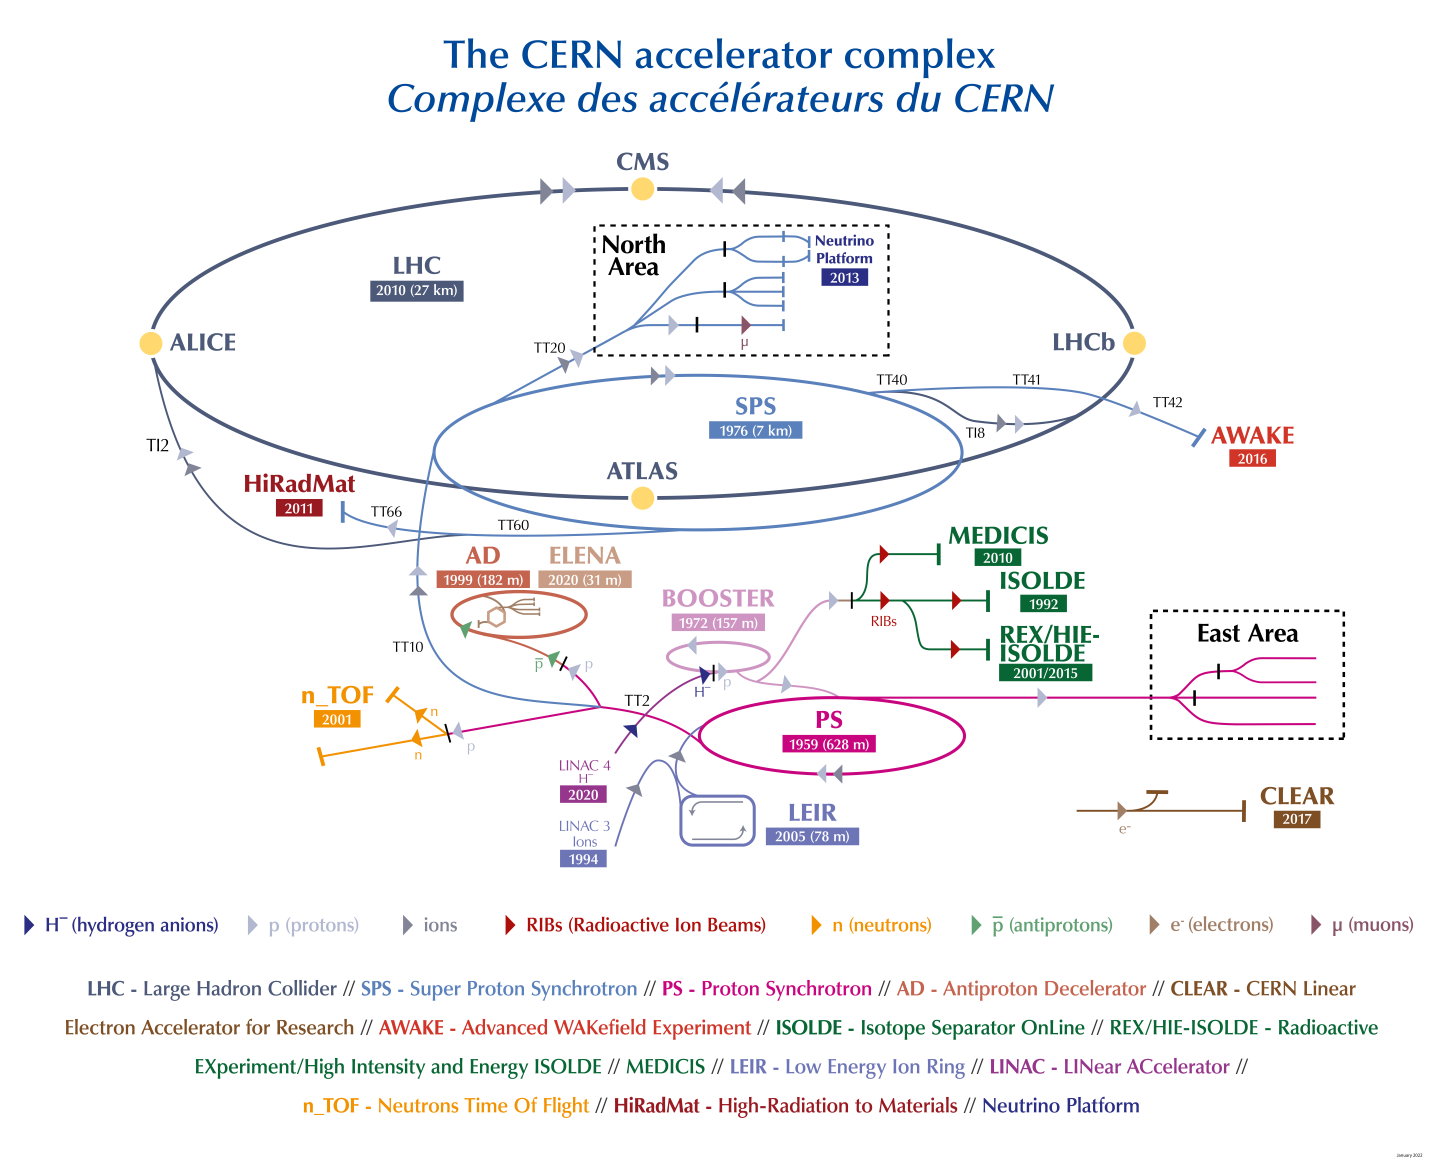
\includegraphics[width=1\textwidth]{Figs/Chapter3/CCC-v2022_Large.png}
	\caption{Schematic representation of the CERN accelerator complex as in 2023. Figure taken from \cite{lopienskaewaCERNAcceleratorComplex2022}.}
	\label{fig:AcceleratorComplex}
\end{figure}

It is noteworthy that the LHC is only the last element of the acceleration chain, as represented in the \fig\ref{fig:AcceleratorComplex}. The beam energy increases gradually using the past CERN's accelerators. Depending on the type of beams (pp or AA), the route to the LHC differs slightly. For a proton beam, negatively charged hydrogen ions are first accelerated by the Linear Accelerator 4 (LINAC 4)\footnote{Until 2020, the first acceleration stage was performed by the LINAC 2 that accelerated hydrogen atoms.} to 160 \mev, and then they are injected in the Proton Synchroton Booster (BOOSTER) in order to reach an energy of 2 \gev. The electrons of the hydrogen ions are removed when leaving the LINAC 4. For a heavy-ion collision, the Linear Accelerator 3 (LINAC 3) provides a beam of heavy-ions -- already stripped of their electrons -- to the Low Energy Ion Ring (LEIR), which accelerates them to 72 \mev per nucleon. Whether it is a beam made of protons or heavy-ions, they are successively accelerated by the PS and SPS up to 450 \gev (or 177 \gev per nucleon for heavy-ions). The particles are finally injected in the rings of the LHC in order to reach their top energy of 6.5 \tev (or 2.56 \tev per nucleon for Pb beams) and collide in the four collision points where sits the four main LHC's experiments: ATLAS, CMS, LHCb, and ALICE\cite{AcceleratorComplexCERN}. \Tab\ref{tab:LHCExperiments} presents a few of their characteristics. 

\begin{table}[!h]
    \centering
    \begin{tabular}{p{3cm}@{\hspace{1cm}} p{2cm}@{\hspace{0.75cm}} p{2cm}@{\hspace{0.75cm}} p{2cm}@{\hspace{0.75cm}} p{2cm}@{}}
    \noalign{\smallskip}\hline\noalign{\smallskip}
    Experiment & ATLAS & CMS & ALICE & LHCb\\
    \noalign{\smallskip}\hline \noalign{\smallskip}
    Participants & 5 991 & 5 824 & 2 085 & 1 585\\
    \noalign{\smallskip}\hline \noalign{\smallskip}
    Height (m) & 25 & 15 & 16 & 10\\
    Length (m) & 46 & 21 & 26 & 21\\
    Width (m) & 25 & 15 & 16 & 13\\
    Weight (tonnes) & 7 000 & 14 000 & 10 000 & 5 600\\
    \noalign{\smallskip}\hline\noalign{\smallskip}
    \end{tabular}
    \caption{A few characteristics of the four main LHC experiments, namely ATLAS, CMS, ALICE and LHCb. The participants include particle physicists, engineers, technicians and students; their number corresponds to the one as of March 2023\cite{Greybook}. The dimensions of each detector originate from \cite{aadATLASExperimentCERN2008}\cite{cmscollaborationCMSExperimentCERN2008}\cite{alicecollaborationALICEExperimentCERN2008}\cite{lhcbcollaborationLHCbDetectorLHC2008}.}\label{tab:LHCExperiments}
\end{table}

A Toroidal LHC Apparatus (ATLAS) and a Compact Muon Solenoid (CMS) are the most colossal experiments at the LHC, as much in terms of the number of participants as in the dimension of their detectors. Both cover a wide range of physics and share the same goals, namely characterising the elementary particles of Standard Model -- in particular, the Higgs boson -- and searching for the new particles beyond the Standard Model, such as dark matter candidates or supersymmetric particles. 

ALICE and LHCb (Large Hadron Collider beauty) are more specialised. ALICE aims at studying QCD matter, and particularly under extreme energy densities where a phase of deconfined quark-gluon matter forms, the QGP. On the other hand, LHCb focuses on heavy flavour physics. It is concerned about new physics in \DIFdelbegin \DIFdel{the }\DIFdelend CP violation and rare decays\DIFdelbegin \DIFdel{of primarily }\DIFdelend \DIFaddbegin \DIFadd{, primarily of }\DIFaddend beauty but also charm hadrons.\\

In order to carry out their physics programme, the LHC must provide different types of beam. For instance, ATLAS and CMS are essentially interested in pp collisions with the highest interaction rate possible, whereas ALICE needs heavy-ion runs to study \textit{directly}\footnote{As discussed in \Sec\ref{subsec:ComparisonPP}, the QGP can also be investigated via the study of its signatures in pp collisions.} the QGP. Therefore, the Run Coordination of each experiment gathers regularly with LHC Programme Coordination to discuss \DIFdelbegin \DIFdel{-- and even negotiate -- }\DIFdelend \DIFaddbegin \DIFadd{and negotiate }\DIFaddend the accelerator schedule\DIFdelbegin \DIFdel{and }\DIFdelend \DIFaddbegin \DIFadd{, in order to }\DIFaddend define a programme which best meets everyone's needs.

\subsection{The accelerator programme}

\begin{table}[!t]
    \centering
    \begin{tabular}{b{2cm}@{\hspace{0.5cm}} b{1cm}@{\hspace{0.75cm}} b{1.5cm}@{\hspace{0.75cm}} b{2.5cm}@{\hspace{0.25cm}} >{\raggedleft\arraybackslash}b{5cm}@{\hspace{0.25cm}}}
    \noalign{\smallskip}\hline\noalign{\smallskip}
    LHC Run & Year & Collision & Centre-of-mass energy (per nucleon) & Dates \\
    \noalign{\smallskip}\hline \noalign{\smallskip}
    \bf Run 1 & 2009 & pp & 900 \gev & 23$^{\textrm{rd}}$ Nov. to 14$^{\textrm{th}}$ Dec.\\
     & & pp & 2.36 \tev & 14$^{\textrm{th}}$ and 16$^{\textrm{th}}$ Dec.\\
    \\
     & 2010 & pp & 7 \tev & 30$^{\textrm{th}}$ Mar. to 4$^{\textrm{th}}$ Nov.\\
     &  & pp & 900 \gev & 2$^{\textrm{nd}}$, 3$^{\textrm{rd}}$ and 27$^{\textrm{th}}$ May\\
     &  & Pb-Pb & 2.76 \tev & 9$^{\textrm{th}}$ Nov. to 6$^{\textrm{th}}$ Dec.\\
     \\

     & 2011 & pp & 7 \tev & 21$^{\textrm{th}}$ Feb. to 4$^{\textrm{th}}$ Nov.\\
     &  & pp & 2.76 \tev & 24$^{\textrm{th}}$ to 27$^{\textrm{th}}$ Mar.\\
     &  & Pb-Pb & 2.76 \tev & 5$^{\textrm{th}}$ Nov. to 7$^{\textrm{th}}$ Dec.\\
     \\
     & 2012 & pp & 8 \tev & 5$^{\textrm{th}}$ Apr. to 16$^{\textrm{th}}$ Dec.\\
     \\
     & 2013 & p-Pb & 5.02 \tev & 20$^{\textrm{th}}$ Jan. to 10$^{\textrm{th}}$ Feb.\\
     & & pp & 2.76 \tev & 11$^{\textrm{th}}$ to 14$^{\textrm{th}}$ Feb.\\

    \noalign{\smallskip}\hline \noalign{\smallskip}

	\bf Run 2 & 2015 & pp & 13 \tev & 3$^{\textrm{rd}}$ Jun. to 19$^{\textrm{th}}$ Nov.\\
     & & pp & 5.02 \tev & 19$^{\textrm{th}}$ to 23$^{\textrm{rd}}$ Nov.\\
     & & Pb-Pb & 5.02 \tev & 24$^{\textrm{th}}$ Nov. to 13$^{\textrm{th}}$ Dec.\\
    \\
     & 2016 & pp & 13 \tev & 23$^{\textrm{rd}}$ Apr. to 26$^{\textrm{th}}$ Oct.\\
     &  & p-Pb & 5.02 \tev & 4$^{\textrm{th}}$ to 17$^{\textrm{th}}$ Nov.\\
     &  &  &  & 4$^{\textrm{th}}$ to 5$^{\textrm{th}}$ Dec.\\
     &  & p-Pb & 8.16 \tev & 18$^{\textrm{th}}$ to 25$^{\textrm{th}}$ Nov.\\
     &  & Pb-p & 8.16 \tev & 26$^{\textrm{th}}$ Nov. to 4$^{\textrm{th}}$ Dec.\\
    \\
     & 2017 & pp & 13 \tev & 23$^{\textrm{rd}}$ May to 26$^{\textrm{th}}$ Nov.\\
     &  & pp & 5.02 \tev & 11$^{\textrm{th}}$ to 21$^{\textrm{st}}$ Nov.\\
     &  & Xe-Xe & 5.44 \tev & 12$^{\textrm{th}}$ Oct.\\
     \\
     & 2018 & pp & 13 \tev & 12$^{\textrm{th}}$ Apr. to 23$^{\textrm{th}}$ Oct.\\
     &  & Pb-Pb & 5.02 \tev & 7$^{\textrm{th}}$ Nov. to 2$^{\textrm{nd}}$ Dec.\\
    \noalign{\smallskip}\hline\noalign{\smallskip}
    \end{tabular}
    \caption{Summary of the LHC Run 1 and 2 physics programmes with the data taking periods in the rightmost column \cite{LHCCommissioning}.}\label{tab:LHCRunProgramm}
\end{table}

\DIFdelbegin \DIFdel{The }\DIFdelend \DIFaddbegin \DIFadd{As shown in the \tab\ref{tab:LHCRunProgramm}, the }\DIFaddend LHC delivers his first collisions on the 23$^{\textrm{rd}}$ of November 2009; these are pp collisions at \sqrtS = 900 \gev. The centre-of-mass energy gradually increases over the years, from 0.9 \tev to 2.36 and then 7 \tev in 2011, and 8 \tev in 2012. The proton-proton programme is complemented by Pb-Pb collisions at \sqrtSnn = 2.76 \tev in November 2010 and 2011, followed in early 2013 by the first p-Pb run at a centre-of-mass energy per nucleon of 5.02 \tev. A few days later, the collider enters in a long shutdown (LS1), marking the end of the first campaign of data taking now called Run-1 (2009-2013). During this period, the LHC undergoes maintenance operations and preparations in view of an increase by a factor two of both energy (reaching \sqrtS = 13 \tev in pp collisions) and luminosity\footnote{This quantity corresponds to a measure of the number of collisions either per unit of time (\textit{instantaneous luminosity}) or over a certain period of time (\textit{integrated luminosity}). In the latter case, it is expressed in inverse barns (\invb) or femtobarns (\invfb).} (bunches of protons are separated by 25 ns instead of 50 ns).

In spring 2015 begins the second campaign of data taking, the LHC Run-2. The latter opens with pp collisions at a record energy of 13 \tev, which will be the default \DIFdelbegin \DIFdel{collisional }\DIFdelend \DIFaddbegin \DIFadd{collision }\DIFaddend energy in pp until the end of the Run-2. The same goes for heavy-ion collisions: the Pb-Pb and p-Pb data are now collected at \sqrtSnn = 5.02 \tev, and up to 8.16 \tev in the latter case. Note also the presence of a short Xe-Xe run at \sqrtSnn = 5.44 \tev in October 2017. The Run-2 comes to an end on December 2018; the LHC enters in its second long shutdown (LS2). As for the LS1, this is the opportunity for the collider and its experiments to be renovated and upgraded. 

On the 5th of July 2022, the LHC restarts and delivers its first pp collisions -- almost four years after the start of the LS2 -- at the new record energy of 13.6 \tev, signalling the beginning of the Run-3.

\section{The ALICE collaboration}
\label{sec:ALICECollaboration}

Amongst the different collaboration based at CERN, ALICE holds a particular place since the work presented in this manuscript has been realised within this experiment. As \DIFdelbegin \DIFdel{mentionned }\DIFdelend \DIFaddbegin \DIFadd{mentioned }\DIFaddend above, it aims at studying the properties of strongly interacting matter and particularly under extreme energy densities where the quark-gluon plasma is formed (\Sec\ref{sec:QGP}). 

\subsection{The collaboration}

As of March 2023, the ALICE collaboration counts 2084 physicists, engineers, technicians and students from 174 institutes in 41 countries. Most of its members originate from Europe (France, Italy, Germany,...), but also from Asia (China, South Korea, Japan,...) and America (United States, Brazil, Mexico,...). In order to coordinate the efforts within the collaboration, ALICE is organised in different boards and committees, each covering a specific scope\footnote{Only a subset of the ALICE management structure is \DIFdelbegin \DIFdel{mentionned}\DIFdelend \DIFaddbegin \DIFadd{mentioned}\DIFaddend . The complete picture is specified in the ALICE Constitution \cite{alicecollaborationALICECollaboration}.}:

\begin{itemize}
\item[$\bullet$] \textit{The Collaboration Board (CB)} is the highest \DIFdelbegin \DIFdel{body of }\DIFdelend \DIFaddbegin \DIFadd{instance of the }\DIFaddend collaboration, it can examine and render a decision on any issues from the construction of the detector to the publication policy. It consists in a legislative assembly, mainly composed of the representatives of each member institute (one per member).
\item[$\bullet$] \textit{The Management Board (MB)} supervises the experiment in any matters (scientific, technical, organisational, operational and financial). It plays the role of the executive authority of the collaboration, and is represented by the Spokesperson and its deputies.
\item[$\bullet$] \textit{The Resource Board (RB)} deals with the financial aspect of ALICE. Each national funding agency has a seat within this committee.
\item[$\bullet$] \textit{The Physics Board (PB)} coordinates the analysis \DIFdelbegin \DIFdel{work }\DIFdelend \DIFaddbegin \DIFadd{efforts }\DIFaddend in order to address the physics goals defined by the CB and MB. It consists in eight Physics Working Groups (PWG), each covering a specific theme, as presented in \tab\ref{tab:PhysicsBoard}.

\begin{table}[h]
    \centering
    \begin{tabular}{p{5cm}@{\hspace{0.5cm}} >{\raggedright\arraybackslash}p{7cm}@{\hspace{0.5cm}}}
    \noalign{\smallskip}\hline\noalign{\smallskip}
	Physics Working Group & Topic\\
    \noalign{\smallskip}\hline \noalign{\smallskip}
    \textit{PWG-CF} & Correlations and Flow\\
	\textit{PWG-DQ} & Dileptons and Quarkonia\\
	\textit{PWG-EM} & Electromagnetic probes\\
	\textit{PWG-HF} & Heavy Flavour\\
	\textit{PWG-JE} & Jets\\
	\textit{PWG-LF} & Light-Flavours\\
	\textit{PWG-MM} & Monte Carlo generators and Minimum bias analysis\\
	\textit{PWG-UD} & Ultra-peripheral collisions and Diffraction\\
    \noalign{\smallskip}\hline\noalign{\smallskip}
    \end{tabular}
    \caption{The eight working groups of the ALICE Physics Board, as of 2023.}\label{tab:PhysicsBoard}
\end{table}

Each PWG is also subdivided in Physics Analysis Group (PAG). For instance, the PWG-Light Flavours includes four PAGs: \textit{Resonances}, \textit{Spectra}, \textit{Nuclei and Exotica}, and \textit{Strangeness}. The present analyses on multi-strange baryons (\chap\ref{chap:CPTAnalysis} and \ref{chap:CorrelatedAnalysis}) are part of the latter group.

\item[$\bullet$] \textit{The Run Coordination (RC)} is responsible for the operation of the ALICE detector. Amongst its duties, it must ensure efficient data taking, optimal data quality and must define the LHC schedule with the LHC Programme Coordination in order to meet the physics goals of the collaboration.
\item[$\bullet$] \textit{The Editorial Board (EB)} manages the publication process (publication, conference proceedings, internal and technical notes). It is complemented by the \textit{Conference Committee (CC)} that oversees the oral presentations (talk or poster) outside of the collaboration.
\end{itemize}

This structure is quite common in high-energy experiments, most of the collaboration \DIFaddbegin \DIFadd{are }\DIFaddend being organised in this way. With different denominations perhaps, but the essence stays the same.

\subsection{The detector}
\label{subsec:ALICEDetector}

The ALICE detector sits in a cavern 56 m below the ground, in the vicinity of Saint-Genis-Pouilly in France. It is located at the interaction point 2 of the LHC, where the L3 experiment at the former LEP collider was installed. From the latter only remains the gigantic red octogonal solenoid magnet, now symbol of the ALICE collaboration.

Being the only experiment dedicated to studying the QGP, ALICE has been designed as general-purpose detector capable of accessing a large number of observables. The physics targets impose several design constraints.

\begin{figure}[!t]
	\centering
	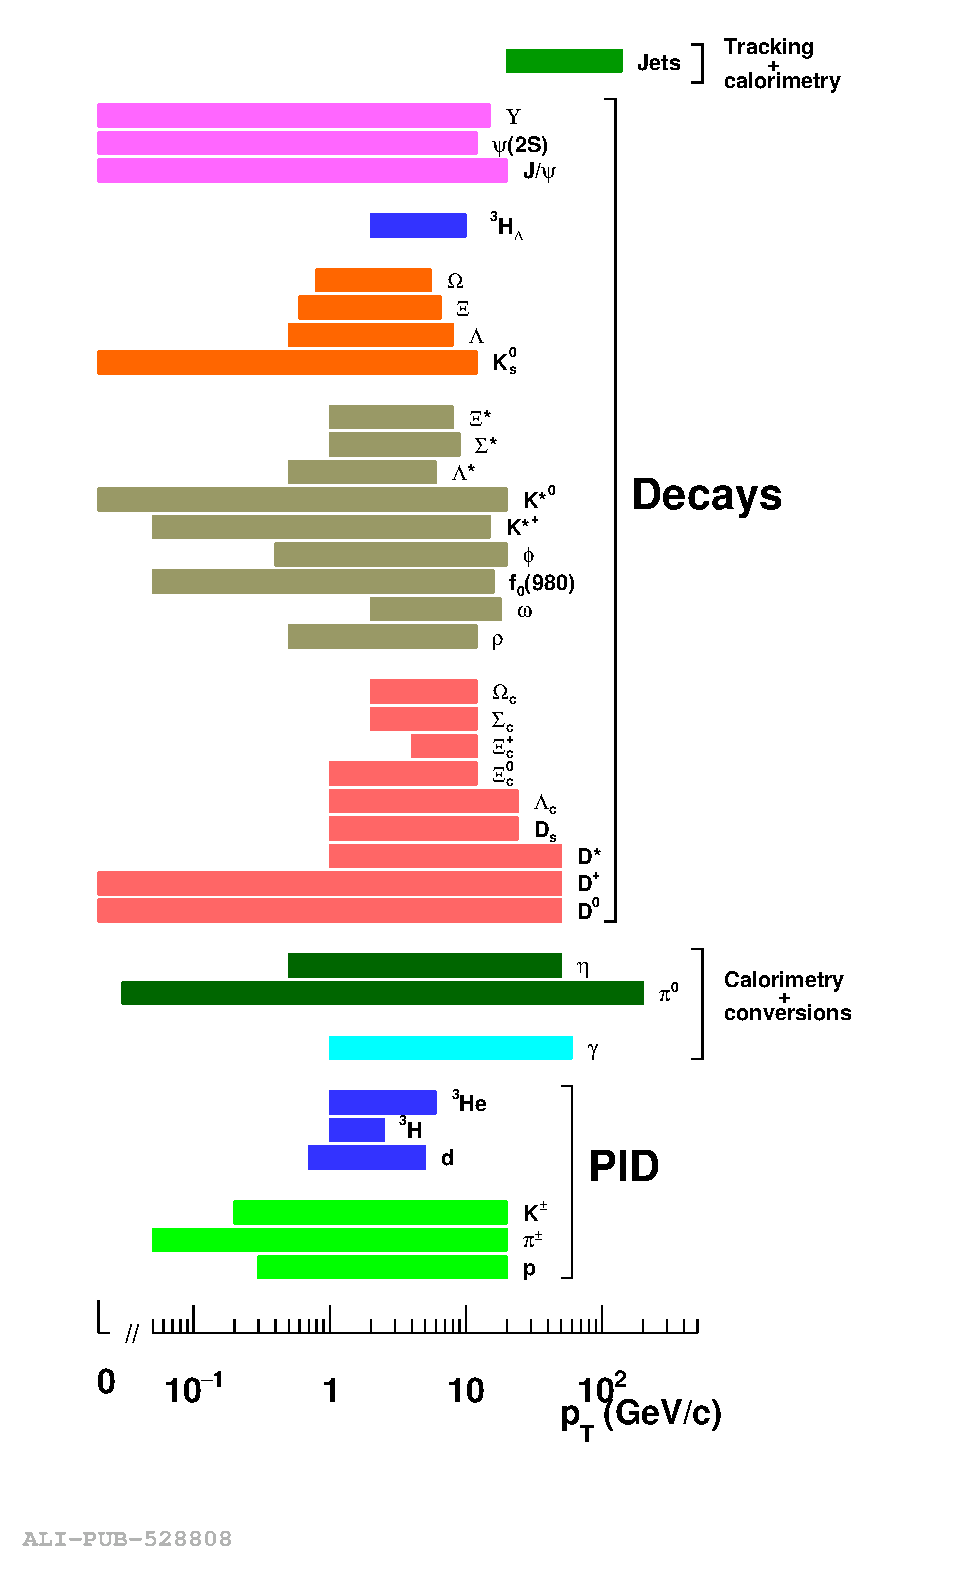
\includegraphics[width=0.85\textwidth]{Figs/Chapter3/ALICE_PID_performance_v3.eps}
	\caption{ALICE particle identification and reconstruction as a function of \pT. Figure taken from \cite{alicecollaborationALICEExperimentJourney2022}.}
	\label{fig:PIDCapabilities}
\end{figure} 

The apparatus must be able to operate in a high-multiplicity environment, considering that the charged particle density per unit of rapidity in the most violent Pb-Pb collisions may reach $\dNchdeta = 2035 \pm 52$ \cite{alicecollaborationCentralityDependenceChargedParticle2016}. For that reason, high granularity detectors -- such as the Inner Tracking System -- are employed to ensure an excellent reconstruction of the primary and secondary vertices, especially close to the interaction point. In fact, the design of ALICE was optimized to endure values up to $\dNchdeta = 4000$, and twice as much in simulations.

To gain as much insights as possible on the QGP evolution, most of the measurements shall be achievable over a wide momentum range, spanning from very low transverse momentum ($\sim$100 \mmom) -- where most of the particle production is -- up to large transverse momentum ($\geq$ 100 \gmom). This requires reducing the multiple scattering at low \pT, and thus using extremely thin detectors. \DIFdelbegin \DIFdel{The }\DIFdelend \DIFaddbegin \DIFadd{At central rapidity, the }\DIFaddend material budget amounts \DIFdelbegin \DIFdel{at central rapidity }\DIFdelend to 13\% radiation length, \Xzero\footnote{This is the characteristic amount of matter over which a high-energy electron loses all its energy by bremsstrahlung (\ie deceleration via the emission of photons) but 1/$e$. It is expressed in g.cm$^{-2}$ \cite{particledatagroupReviewParticlePhysics2022}.}, up to Time Projection Chamber outter wall\footnote{Here, there are two antogonistic constraints: the detectors must be thin and radiation tolerant in order to function in a high-multiplicity environment, the latter requiring relatively thick materials. However, in ALICE, the interaction rate in heavy-ion collisions is low (about 10 kHz or 10 000 Pb-Pb collisions per second) such that the radiation doses are rather mild, compared with the levels in ATLAS and CMS (790 and 840 kGy respectively): the total dose over the period of a LHC-Run varies between tens of Gy for the furthest parts of the Inner Tracking System to 2.7 kGy close to the interaction point.}. For comparison, it is about 47\% and 40\% \Xzero in ATLAS and CMS at the end of their inner tracker \cite{aadATLASExperimentCERN2008}\cite{cmscollaborationCMSExperimentCERN2008}, and 17.5\% \Xzero down to the VELO (VErtex LOcator) for LHCb \cite{lhcbcollaborationLHCbDetectorLHC2008}. At high \pT, the constraint lies in the need for a good resolution at large transverse momentum. This is achieved by means of a large tracking lever arm thanks to the Time Projection Chamber, that extends up to 2.5 m. 

\DIFdelbegin \DIFdel{That }\DIFdelend \DIFaddbegin \DIFadd{This }\DIFaddend brings an extra consideration. In order to avoid excessivily bending the low \pT charged particles and making them impossible to detect, the momentum measurement down to 100 \mmom necessitates a moderate magnetic field of 0.5 T\footnote{Among the four main LHC experiments, this is the most moderate magnetic field. For comparison, CMS uses a magnetic field of 4 T, the same as the LHCb dipole magnet, and ATLAS solenoid magnet delivers a 2 T field.}. In return, the high \pT charged particles are less curved resulting in a reduction of the momentum resolution, when they are still measurable. 

Along the same line, many observables depend on the nature of the particle, and so it is essential to have a robust particle identification (PID) over a wide momentum range. To that end, ALICE exploits all the PID techniques on the market: ionization energy loss in the Time Projection Chamber, time-of-flight measurement with the Time-Of-Flight detector, Cerenkov and transition radiations in the High-Momentum Particle Identification Detector \DIFaddbegin \DIFadd{(HMPID) }\DIFaddend and Transition Radiation Detector \DIFaddbegin \DIFadd{(TRD) }\DIFaddend respectively, energy measurement with the Electromagnetic Calorimeters \DIFaddbegin \DIFadd{(EMCal) }\DIFaddend and the Photon Spectrometer \DIFaddbegin \DIFadd{(PHOS)}\DIFaddend . The \fig\ref{fig:PIDCapabilities} provides an overview of the PID and reconstruction capabilities with the transverse momentum coverage.\\


\Fig\ref{fig:ALICEdetector} provides a overview of the different elements of the detector. It comprises 19 detection systems organised in two groups: the ones in the central barrel at mid-rapidity ($|\eta| < 0.9$), embedded in the L3 solenoid magnet that delivers a homogenous magnetic field up to 0.5 T; the others at forward rapidity ($-4 < \eta < -2.5$), dedicated to muon detection. An exhaustive description of the ALICE apparatus can be found in \cite{alicecollaborationALICEExperimentCERN2008}, as well as its physics performances in \cite{carminatiALICEPhysicsPerformance2004}\cite{alicecollaborationALICEPhysicsPerformance2006}\cite{alicecollaborationPerformanceALICEExperiment2014}. In the next paragraphs, we will concentrate on the main detectors employed in this thesis, namely the Inner Tracking System (\DIFaddbegin \DIFadd{\Sec}\DIFaddend \ref{subsubsec:ITS}), the Time Projection Chamber (\DIFaddbegin \DIFadd{\Sec}\DIFaddend \ref{subsubsec:TPC}), the VZERO (\DIFaddbegin \DIFadd{\Sec}\DIFaddend \ref{subsubsec:VZERO}) and the Time-Of-Flight detector (\DIFaddbegin \DIFadd{\Sec}\DIFaddend \ref{subsubsec:TOF}). 

Before proceeding, a note on the location of the different parts of the apparatus: in the cartesian coordinate system of ALICE, the origin lies at the centre of the central barrel and the $z$-axis coincides with the beams. The elements located on positive $z$ belongs to the A-side (\DIFdelbegin \DIFdel{Anti clockwise, beam going }\DIFdelend \DIFaddbegin \DIFadd{beam circulating in Anti-clockwise direction, }\DIFaddend from ALICE to the ATLAS interaction point), the others with negative $z$ are on the C-side (\DIFdelbegin \DIFdel{Clockwise, beam going }\DIFdelend \DIFaddbegin \DIFadd{beam going in Clockwise direction, }\DIFaddend from ALICE to the CMS interaction point). The $y$-axis points towards the top of the detector and the $x$-axis is in the horizontal plane, going towards the centre of the LHC ring. Moreover, there exists a cylindrical coordinates system based on the distance from the origin $r$ and the azimuthal angle $\varphi$ in the transverse plane $xy$, as well as a spherical one with an additional angle, the zenithal angle denoted $\theta$.


\begin{figure}[t]
	\centering
	\includegraphics[width=1\textwidth]{Figs/Chapter3/ALICE.png}
	\caption{Schematic representation of the ALICE apparatus, as it was operated in the LHC Run-2. Figure taken from \cite{alicecollaborationALICEExperimentJourney2022}.}
	\label{fig:ALICEdetector}
\end{figure}


\subsubsection{Inner Tracking System}
\label{subsubsec:ITS}

The Inner Tracking System (ITS) of ALICE is the closest detection system to the interaction point. It surrounds the beam pipe, a 800 \mum-thick beryllium cylinder with \DIFdelbegin \DIFdel{a }\DIFdelend \DIFaddbegin \DIFadd{an average }\DIFaddend radius of 2.9 \cm. The ITS is designed in order to i) estimate the primary vertex position to a precision better than 100 \mum, ii) reconstruct secondary decay vertices of relatively short lifetime particles such as hyperons, D or B mesons, iii) track and identify particles whose $\pT \leq 200 \mmom$, iv) bring constraints on the particles reconstructed by the Time Projection Chamber and, by so doing, improve the momentum and angle resolution, v) enhance PID capabilities of the ALICE apparatus, and finally vi) provide additionnal trigger information. As shown on the \fig\ref{fig:ITSstructure}, the ITS is made of six coaxial cylindrical layers of silicon detectors based on three different technologies. The two innermost layers are the Silicon Pixel Detectors (SPD), followed by the two layers of Silicon Drift Detector (SDD). The two outermost layers utilizes Silicon Strip Detectors (SSD). The number of detector, and their positionning, has been optimized in order to guarantee efficient track reconstruction and highly precise estimation of the impact parameter. The pseudo-rapidity coverage varies from a layer to another, but taken as a whole, the ITS covers a range of $|\eta| < 0.9$ for all interaction point within $\pm$ 5.3 \cm along the beam direction. Its overall material budget of 7.18\% \Xzero (including the silicon detectors, thermal shields, electronics, support structure, cooling system) makes it the only device capable of detecting low-\pT particles, with a relative momentum resolution better than 2\% for pions with momentum between 100 \mmom and 3 \gmom. Some important characteristics of the ITS are reported in \tab\ref{tab:ITSspec}.

\begin{figure}[t]
\begin{center}
\subfigure[]
{
	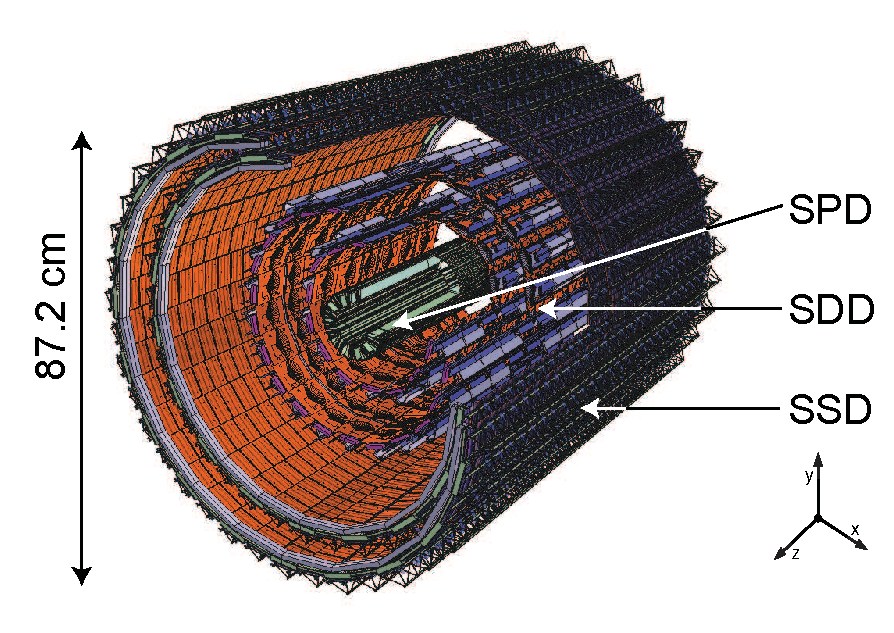
\includegraphics[width=0.75\textwidth]{Figs/Chapter3/its-rf-2-26925.eps}
}
\end{center}
\subfigure[]
{
	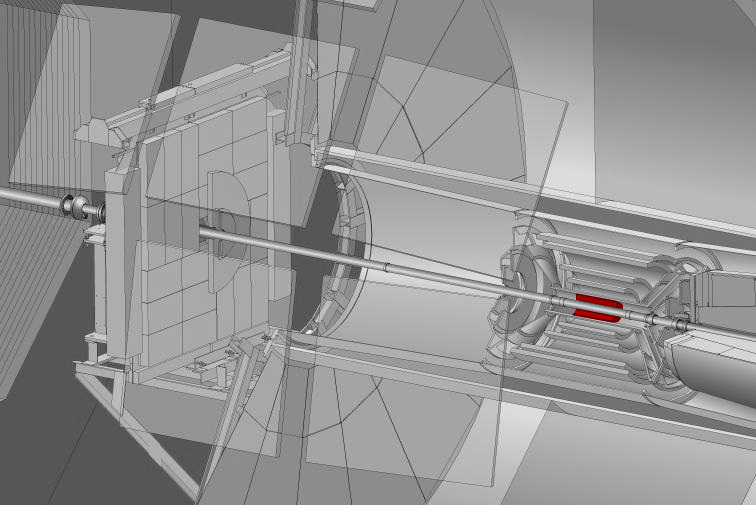
\includegraphics[width=0.31\textwidth]{Figs/Chapter3/ALICE-3D-Run1+2-ITS+V0-Inlay-v0-2012-08-02-Highlight-SPD.png}
}
\subfigure[]
{
	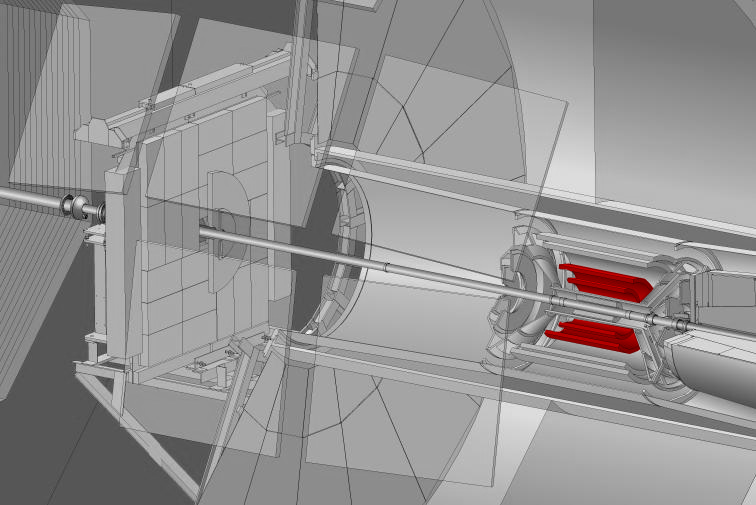
\includegraphics[width=0.31\textwidth]{Figs/Chapter3/ALICE-3D-Run1+2-ITS+V0-Inlay-v0-2012-08-02-Highlight-SDD.png}
}
\subfigure[]
{
	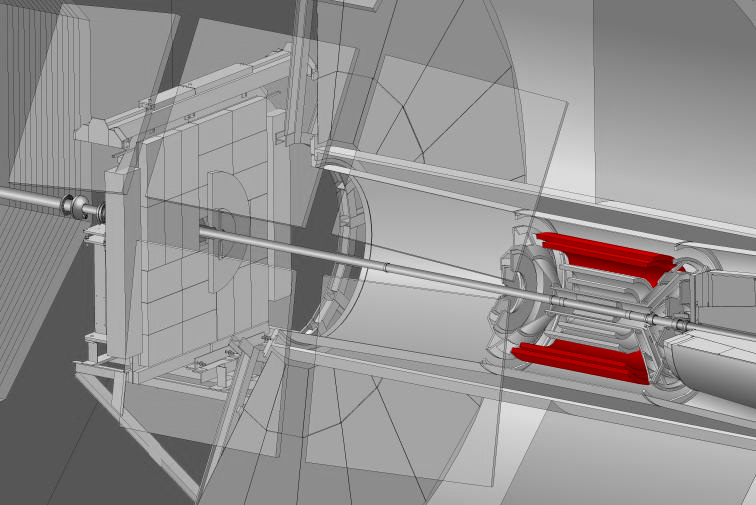
\includegraphics[width=0.31\textwidth]{Figs/Chapter3/ALICE-3D-Run1+2-ITS+V0-Inlay-v0-2012-08-02-Highlight-SSD.png}
}
	\caption{Visualisation of the complete structure of the ITS detector (a), as well as a highlight on the SPD(b), SDD(c) and SSD(d) locations in the ALICE apparatus. Figures taken from \cite{alicecollaborationAlignmentALICEInner2017}\cite{maireALICESubdetectorsHighlighted2017}.}
	\label{fig:ITSstructure}
\end{figure}

\begin{table}[t]
    \centering
    \begin{tabular}{b{1.5cm}@{\hspace{0.5cm}} b{1.5cm}@{\hspace{0.25cm}} b{1.5cm}@{\hspace{0.5cm}} b{2cm}@{\hspace{0.5cm}} b{2cm}@{\hspace{0.5cm}} b{1.5cm}@{\hspace{1cm}} b{2cm}@{\hspace{0.cm}}}
    \noalign{\smallskip}\hline\noalign{\smallskip}
	Layer & $r$ (\cm) & $\pm z$ (\cm) & Area ($\m^{2}$) & Active area per module ($\mm^{2}$) & Resolution $r\varphi \times z$ ($\mum^{2}$) & Material budget (\%\Xzero) \\
    \noalign{\smallskip}\hline \noalign{\smallskip}
    1 - SPD & 3.9 & 14.1 & 0.07 & 12.8 $\times$ 69.6 & 12 $\times$ 100 & 1.14 \\
    2 - SPD & 7.6 & 14.1 & 0.14 & 12.8 $\times$ 69.6 & 12 $\times$ 100 & 1.14 \\
    3 - SDD & 15.0 & 22.2 & 0.42 & 72.5 $\times$ 75.3 & 35 $\times$ 25 & 1.13 \\
    4 - SDD & 23.9 & 29.7 & 0.89 & 72.5 $\times$ 75.3 & 35 $\times$ 25 & 1.26 \\
    5 - SSD & 38.0 & 43.1 & 2.20 & 73 $\times$ 40 & 20 $\times$ 820 & 0.83 \\
    6 - SSD & 43.0 & 48.9 & 2.80 & 73 $\times$ 40 & 20 $\times$ 820 & 0.86 \\
    \noalign{\smallskip}\hline\noalign{\smallskip}
    \end{tabular}
    \caption{Details on the six layers of the ITS during the LHC Run-1 and Run-2. \cite{alicecollaborationALICEExperimentCERN2008}\cite{carminatiALICEPhysicsPerformance2004}. The radial distance $r$ are, in fact, average positions. The rightmost column only includes the material budget of the sensor.}\label{tab:ITSspec}
\end{table}

The two innermost layers are positionned at 3.9 and 7.6 \cm from the origin, covering a pseudo-rapidity range of $|\eta| < 2$ and $|\eta| < 1.4$ respectively. At this distance, the track density can reach values up to 80 tracks/$\cm^{2}$. In order to cope with these high track densities, the layers are equipped with SPD employing hybrid\footnote{The term \textit{hybrid} here refers to a type of pixel technology in which the silicon sensor and the readout chip are processed separatedly and connected together via a bump-bonding process. In this way, the detector (silicon sensor) and the electronics (readout chip) can be optimized individually. In LHC experiments, the optimisation is performed such that the detector has a good radiation tolerance and the readout is fast. In return, the assembly tends to be more complex and expensive, the readout chips dissipate a lot of power requiring an efficient cooling system and so more material budget.} silicon pixels. It consists of a bi-dimensional matrix of 256 $\times$ 160 cells of dimension 50 \mum ($r\varphi$) by 425 \mum ($z$). Two matrices are mounted together along the $z$ direction, forming a 141.6 \mm long half-stave. Two of them are attached head to head along the beam direction on a carbon-fibre support with cooling tubes in order to forge a stave. The latter are arranged in ten sectors surrounding the beam pipe, each sector supporting two staves for the inner layer and four for the outer layer. While the high granularity of the SPD provides a spatial resolution of 12 \mum in $r\varphi$ and 100 \mum along $z$, its fast integration time of 100 \nsec -- corresponding to four consecutive bunch-crossings in pp collisions or one in heavy-ions operation -- offers additionnal trigger information.

The SDDs equip the two intermediate layers at an average distance of 15.0 and 23.9 \cm, where the track density rises up to 7 tracks/$\cm^{2}$. Both layers have a pseudo-rapidity acceptance of $|\eta| < 0.9$. The basic module consists in a sensitive area of 70.17 $\times$ 75.26 $\mm^{2}$, split into two drift regions by a central cathode strip at high voltage such that the drift velocity is 8.1 $\mum/\nsec$. At this speed, charges drift to one of the 256 collection anodes (with a 294 \mum pitch) in a maximum time of 4.3 \musec, making it the slowest ITS detector. The SSD modules are mounted on triangular support structure made of carbon-fibre called ladders. The third layer counts 14 ladders with six modules each, and 22 ladders with eight detectors each for the fourth layer. They yield to a spatial precision of 35 \mum in the transverse plane and 25 \mum along the beam axis. \DIFaddbegin \DIFadd{Because of the sensitivity of the SDD layers to temperature changes, two thermal shields surround them in order to avoid any radiation of heat.
}\DIFaddend 

The two outermost layers are constituted of double sided SSD of 73 $\times$ 40 $\mm^{2}$, where each side has 768 parallel strips (with a pitch of 95 \mum) and corresponds to a side of a p-n junction. The p-side (n-side) of the fifth layer (sixth layer) faces the inside of the ITS. The strips from one side are rotated by a stereo angle of 35 mrad with respect to the other, to reduce the overlapping between the strips and thus the number of ambiguities. The SSD modules are assembled on the same ladder design as those of the intermediate layers: 34 ladders, supporting 22 modules each, are installed on average at 38 \cm from the beam pipe for the inner layer and 38 ladders, holding 25 modules each, at 43 \cm for the outer layer. Both covers a pseudo-rapidity region of $|\eta| < 0.9$. The SSDs layers provide a spatial resolution of the track position of 20 \mum in the $r\varphi$ direction and 820 \mum along $z$, which is essential for the track matching from the Time Projection Chamber to the ITS. Similarly to the SDD layers, its analogue readout allows for the measurement of the charge deposited by the passage of a charged particle, and hence opens the door for PID of low-momentum particles.


\DIFdelbegin \DIFdel{Because of the sensitivity of the SDD layers to temperature changes, two thermal shields surround them in order to avoid any radiation of heat.
}%DIFDELCMD < 

%DIFDELCMD < %%%
\DIFdelend \subsubsection{Time Projection Chamber}
\label{subsubsec:TPC}

\DIFdelbegin %DIFDELCMD < \begin{figure}[t]
%DIFDELCMD < \subfigure[]
%DIFDELCMD < {
%DIFDELCMD < 	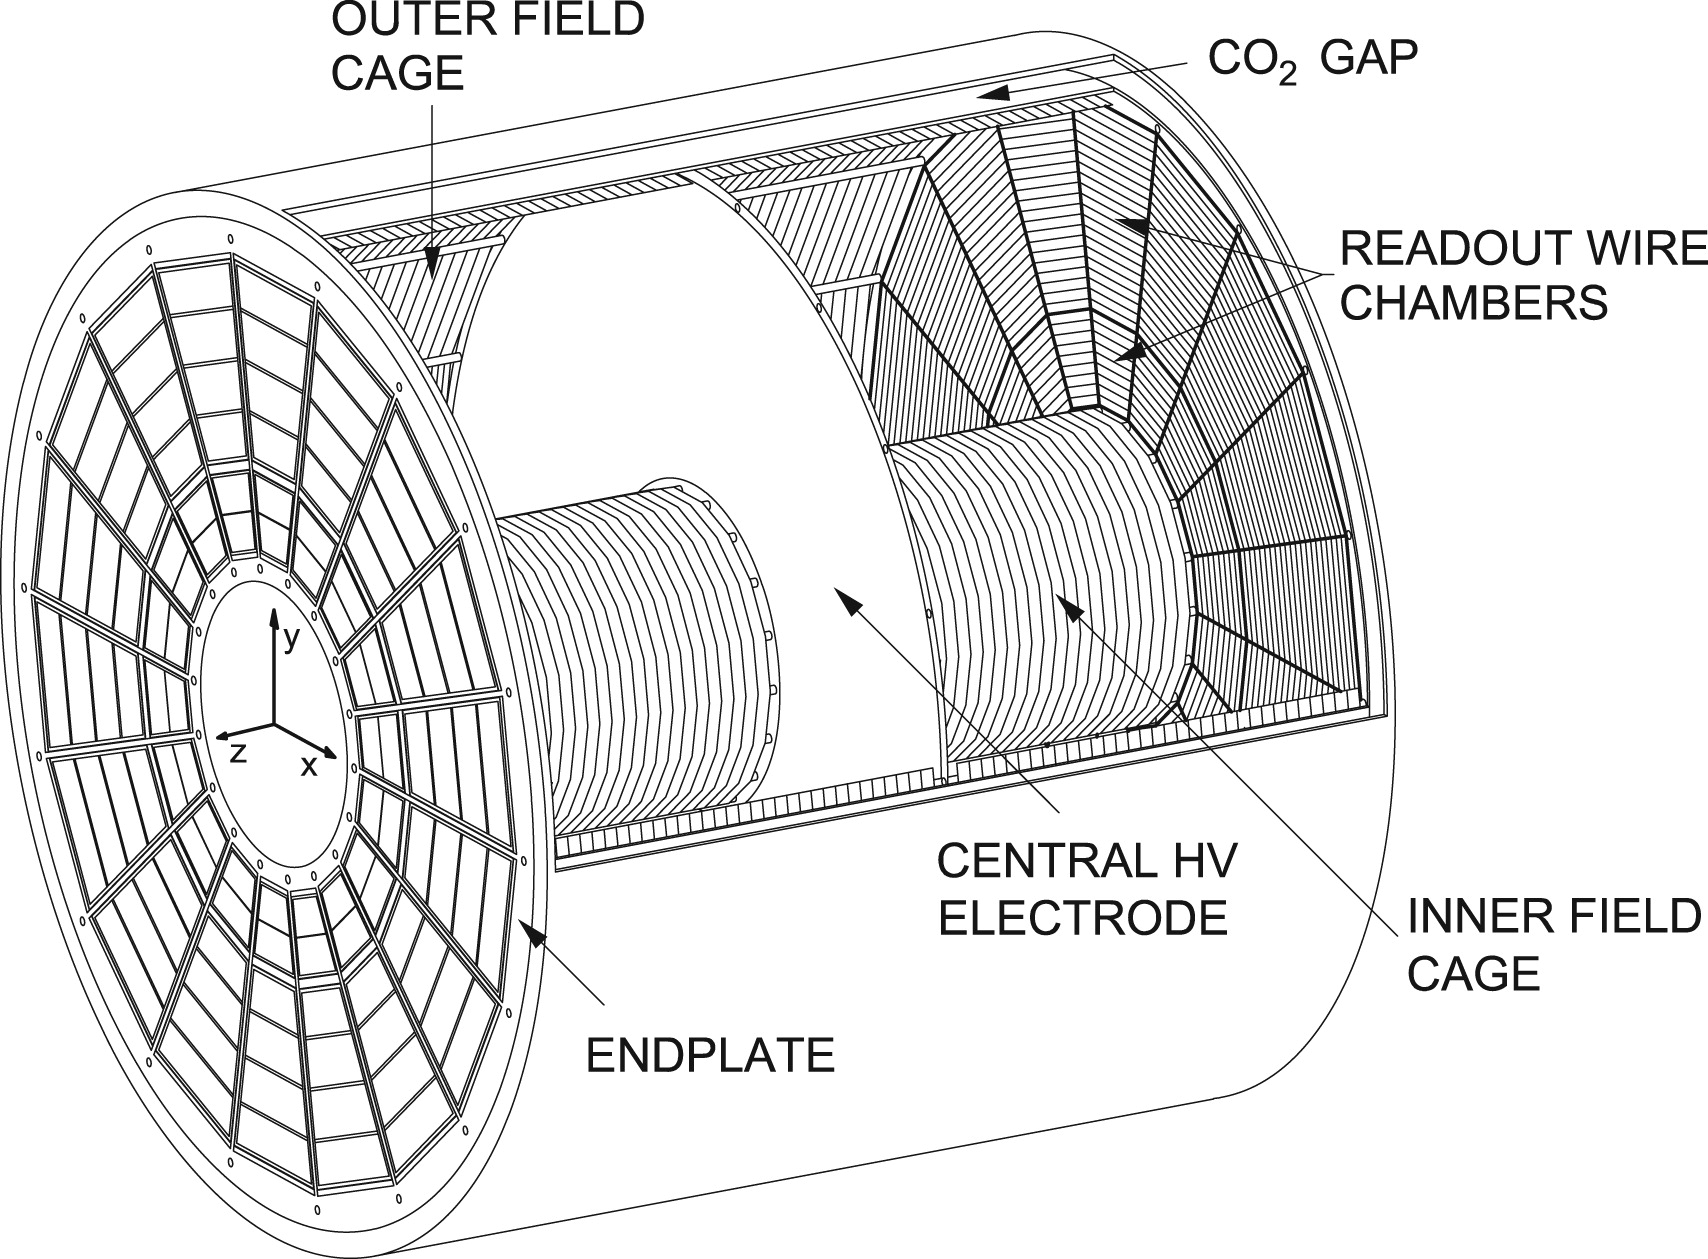
\includegraphics[width=0.62\textwidth]{Figs/Chapter3/1-s2.0-S0168900210008910-gr2_lrg.jpg}
%DIFDELCMD < 	\label{fig:TPCFieldCage}
%DIFDELCMD < }
%DIFDELCMD < \subfigure[]
%DIFDELCMD < {
%DIFDELCMD < 	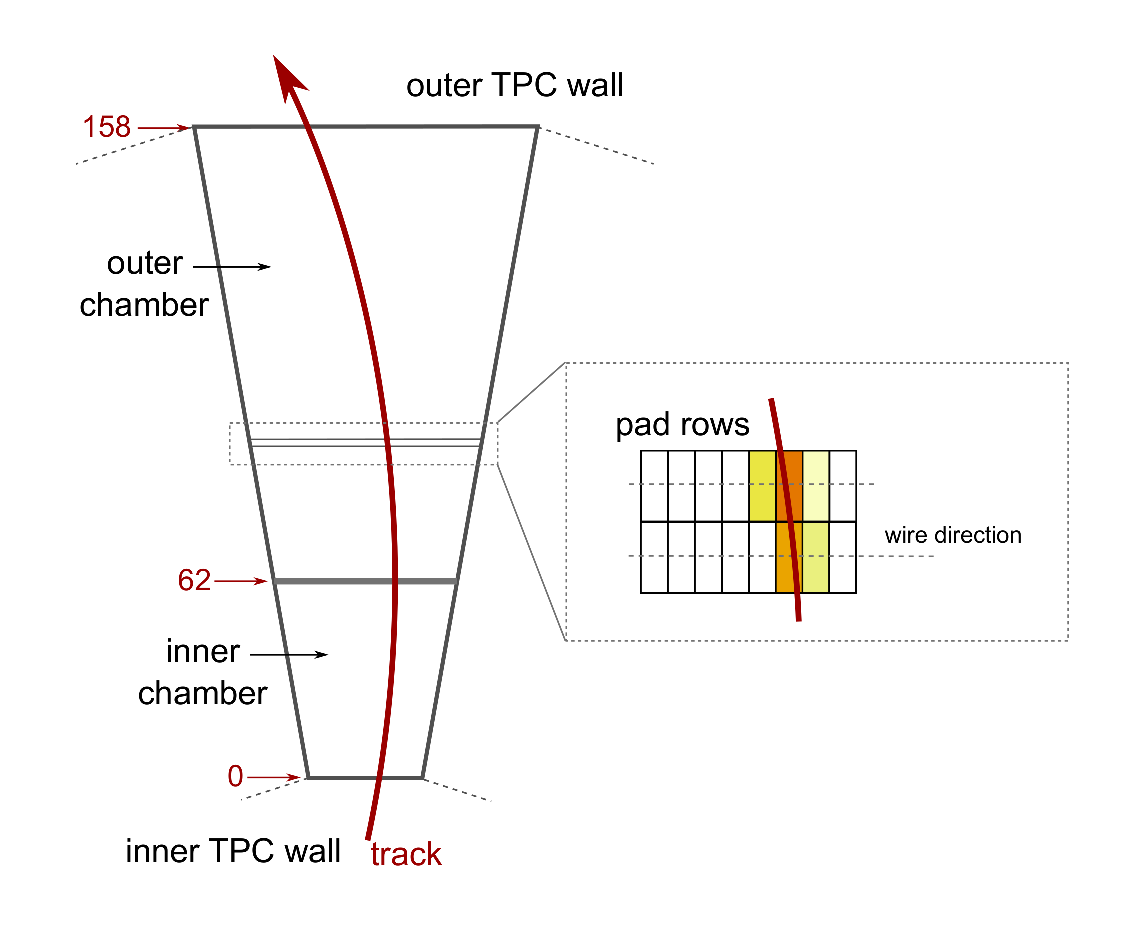
\includegraphics[width=0.50\textwidth]{Figs/Chapter3/Schema-TPC-SecteurEtPadRow.eps}
%DIFDELCMD < 	\label{fig:TPCSector}
%DIFDELCMD < }
%DIFDELCMD < 	%%%
%DIFDELCMD < \caption{%
{%DIFAUXCMD
\DIFdelFL{(Left panel) Scheme of the TPC field cage, taken from \mbox{%DIFAUXCMD
\cite{almeALICETPCLarge2010}}\hspace{0pt}%DIFAUXCMD
. (Right panel) Passage of a charged particle through a sector of the TPC. Figure taken from \mbox{%DIFAUXCMD
\cite{maireALICETPCSectors2011}}\hspace{0pt}%DIFAUXCMD
.}}
	%DIFAUXCMD
%DIFDELCMD < \label{fig:TPCDetector}
%DIFDELCMD < \end{figure}
%DIFDELCMD < 

%DIFDELCMD < %%%
\DIFdelend The Time Projection Chamber (TPC) is main tracking device of the ALICE \DIFdelbegin \DIFdel{experiment}\DIFdelend \DIFaddbegin \DIFadd{detector}\DIFaddend . It is responsible for measuring the momentum of charged particle above 150 \mmom, as well as providing particle identification and \DIFdelbegin \DIFdel{vertex determination}\DIFdelend \DIFaddbegin \DIFadd{primary vertex determination (addressed in more details in \Sec\ref{subsubsec:FinalVertexDet})}\DIFaddend . The TPC design is shown in \fig\ref{fig:TPCFieldCage}. It consists in a cylindrical gaseous detector, \DIFdelbegin \DIFdel{encercling }\DIFdelend \DIFaddbegin \DIFadd{surrounding }\DIFaddend the ITS, with an inner radius of about 85 \cm, an outer radius of 250 \cm and an overall length of 500 \cm along the beam axis. The acceptance of the TPC covers pseudo-rapidities from $|\eta| < 0.9$ (for tracks traversing radially the entire ALICE detector) up to $|\eta| = 1.5$ and the full azimuth (except for the dead zones between sectors). Although \DIFdelbegin \DIFdel{this detector occupies a large volume}\DIFdelend \DIFaddbegin \DIFadd{it is the largest sub-detector of ALICE}\DIFaddend , its material budget remains \DIFaddbegin \DIFadd{quite }\DIFaddend low (about 3.5\% \Xzero).

\DIFaddbegin \begin{figure}[t]
\subfigure[]
{
	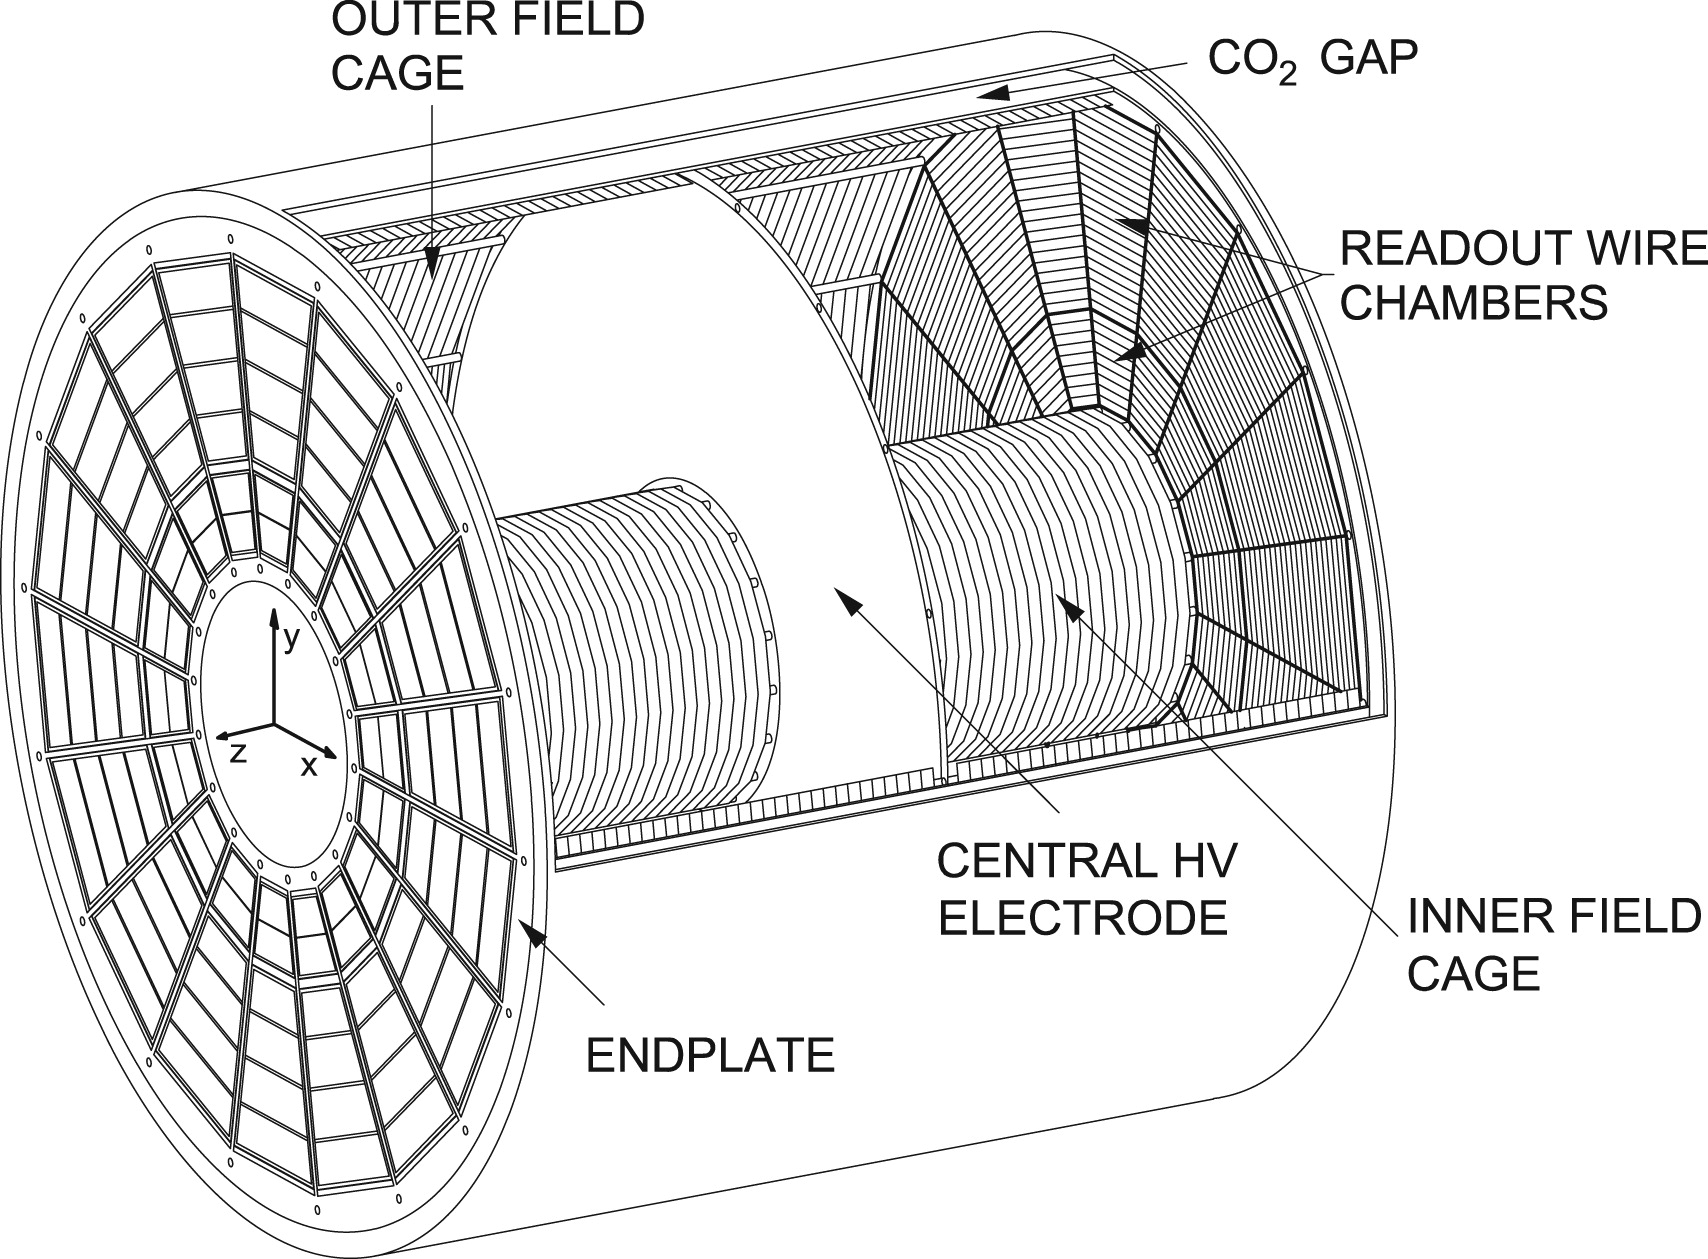
\includegraphics[width=0.62\textwidth]{Figs/Chapter3/1-s2.0-S0168900210008910-gr2_lrg.jpg}
	\label{fig:TPCFieldCage}
}
\subfigure[]
{
	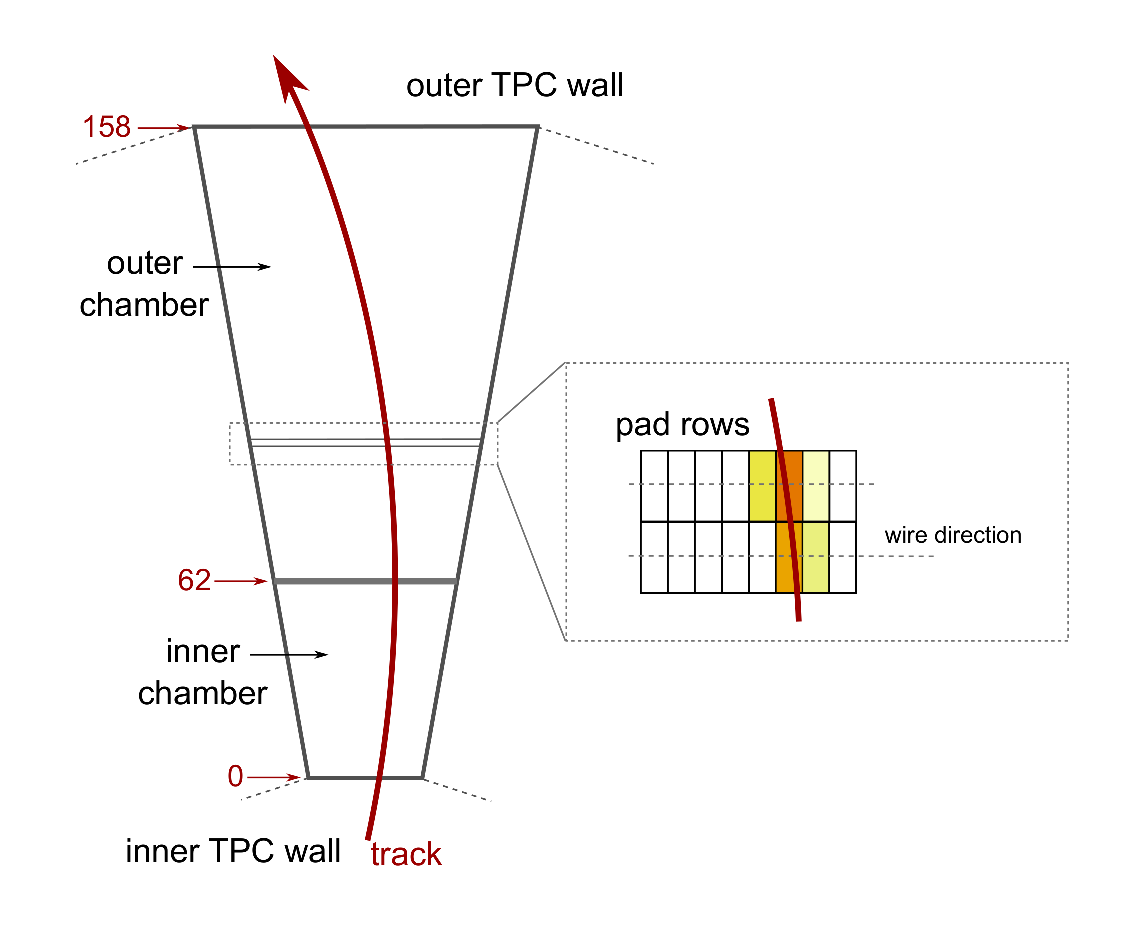
\includegraphics[width=0.50\textwidth]{Figs/Chapter3/Schema-TPC-SecteurEtPadRow.eps}
	\label{fig:TPCSector}
}
	\caption{\DIFaddFL{(Left panel) Scheme of the TPC field cage, taken from \mbox{%DIFAUXCMD
\cite{almeALICETPCLarge2010}}\hspace{0pt}%DIFAUXCMD
. (Right panel) Passage of a charged particle through a sector of the TPC. Figure taken from \mbox{%DIFAUXCMD
\cite{maireALICETPCSectors2011}}\hspace{0pt}%DIFAUXCMD
.}}
	\label{fig:TPCDetector}
\end{figure}

\DIFaddend The detection volume corresponds to a field cage filled with gas and separated in two equal parts, along the beam axis, by a central electrode at -100 kV. At this high voltage, this central membrane generates an axial electrostatic field of 400 V/\cm. When a charged particle traverses the 88 $\m^{3}$ \DIFaddbegin \DIFadd{of TPC's }\DIFaddend active volume, it creates electron-hole pairs along its path by ionisation of the gas. The electrostatic field forces the electrons to drift from the central electrode to the end plates, where they are collected, in a maximum time of 92 \musec at a speed of 2.7 \cm/\musec (depending on the gas composition).

Each end plate is segmented into 18 trapezoidal sectors (as represented in \fig\ref{fig:TPCSector}), being themselves instrumented with two multi-wire proportionnal chambers (MWPC) with cathode pad readout: one stretches from $R= 84.8$ \cm to 132 \cm (inner chamber), the other \DIFdelbegin \DIFdel{ranges }\DIFdelend from 134.6 \cm to 246.6 \cm (outer chamber). This is motivated by the variation of the track density with the \DIFdelbegin \DIFdel{radius}\DIFdelend \DIFaddbegin \DIFadd{radial distance (from the primary vertex)}\DIFaddend , that requires MWPCs with different wire geometry and pad sizes (granularities). Together, the two chambers count a total of 159 readout pad rows: 63 of 4 $\times$ 7.5 $\mm^{2}$ for the inner chamber, 64 of 6 $\times$ 10 $\mm^{2}$ and 32 of 6 $\times$ 15 $\mm^{2}$ for the outer chamber. They measure the deposited charge, as well as the radial position and the drift time. The longitudinal coordinate is inferred from the latter, provided that the drift speed is uniform over the whole volume\footnote{The longitudinal position is \DIFdelbegin \DIFdel{thus }\DIFdelend given by the product of the drift velocity and the drift time\DIFaddbegin \DIFadd{, $v_{\rm drift} \cdot t_{\rm drift}$}\DIFaddend .}. In fact, the gas composition has been optimised for high and stable drift velocity, as well as low diffusion and small radiation length. At the start of the LHC Run-2, a mixture of Ne/CO$_{2}$/N$_{2}$ (90/10/5\%) was employed\DIFdelbegin \DIFdel{until 2017. It was later changed }\DIFdelend \DIFaddbegin \DIFadd{. For the data taking campaign of 2017, it was replaced }\DIFaddend for Ar/CO$_{2}$ (90/10\%) \DIFdelbegin \DIFdel{as the latter reduces the }\DIFdelend \DIFaddbegin \DIFadd{before switching back to the initial gas composition in 2018, as it turns out that the latter yields to a reduced }\DIFaddend space-charge distortion\DIFdelbegin %DIFDELCMD < [%%%
\DIFdel{ref?}%DIFDELCMD < ]%%%
\DIFdelend .

\DIFdelbegin %DIFDELCMD < \begin{figure}[t]
%DIFDELCMD < 	\centering
%DIFDELCMD < 	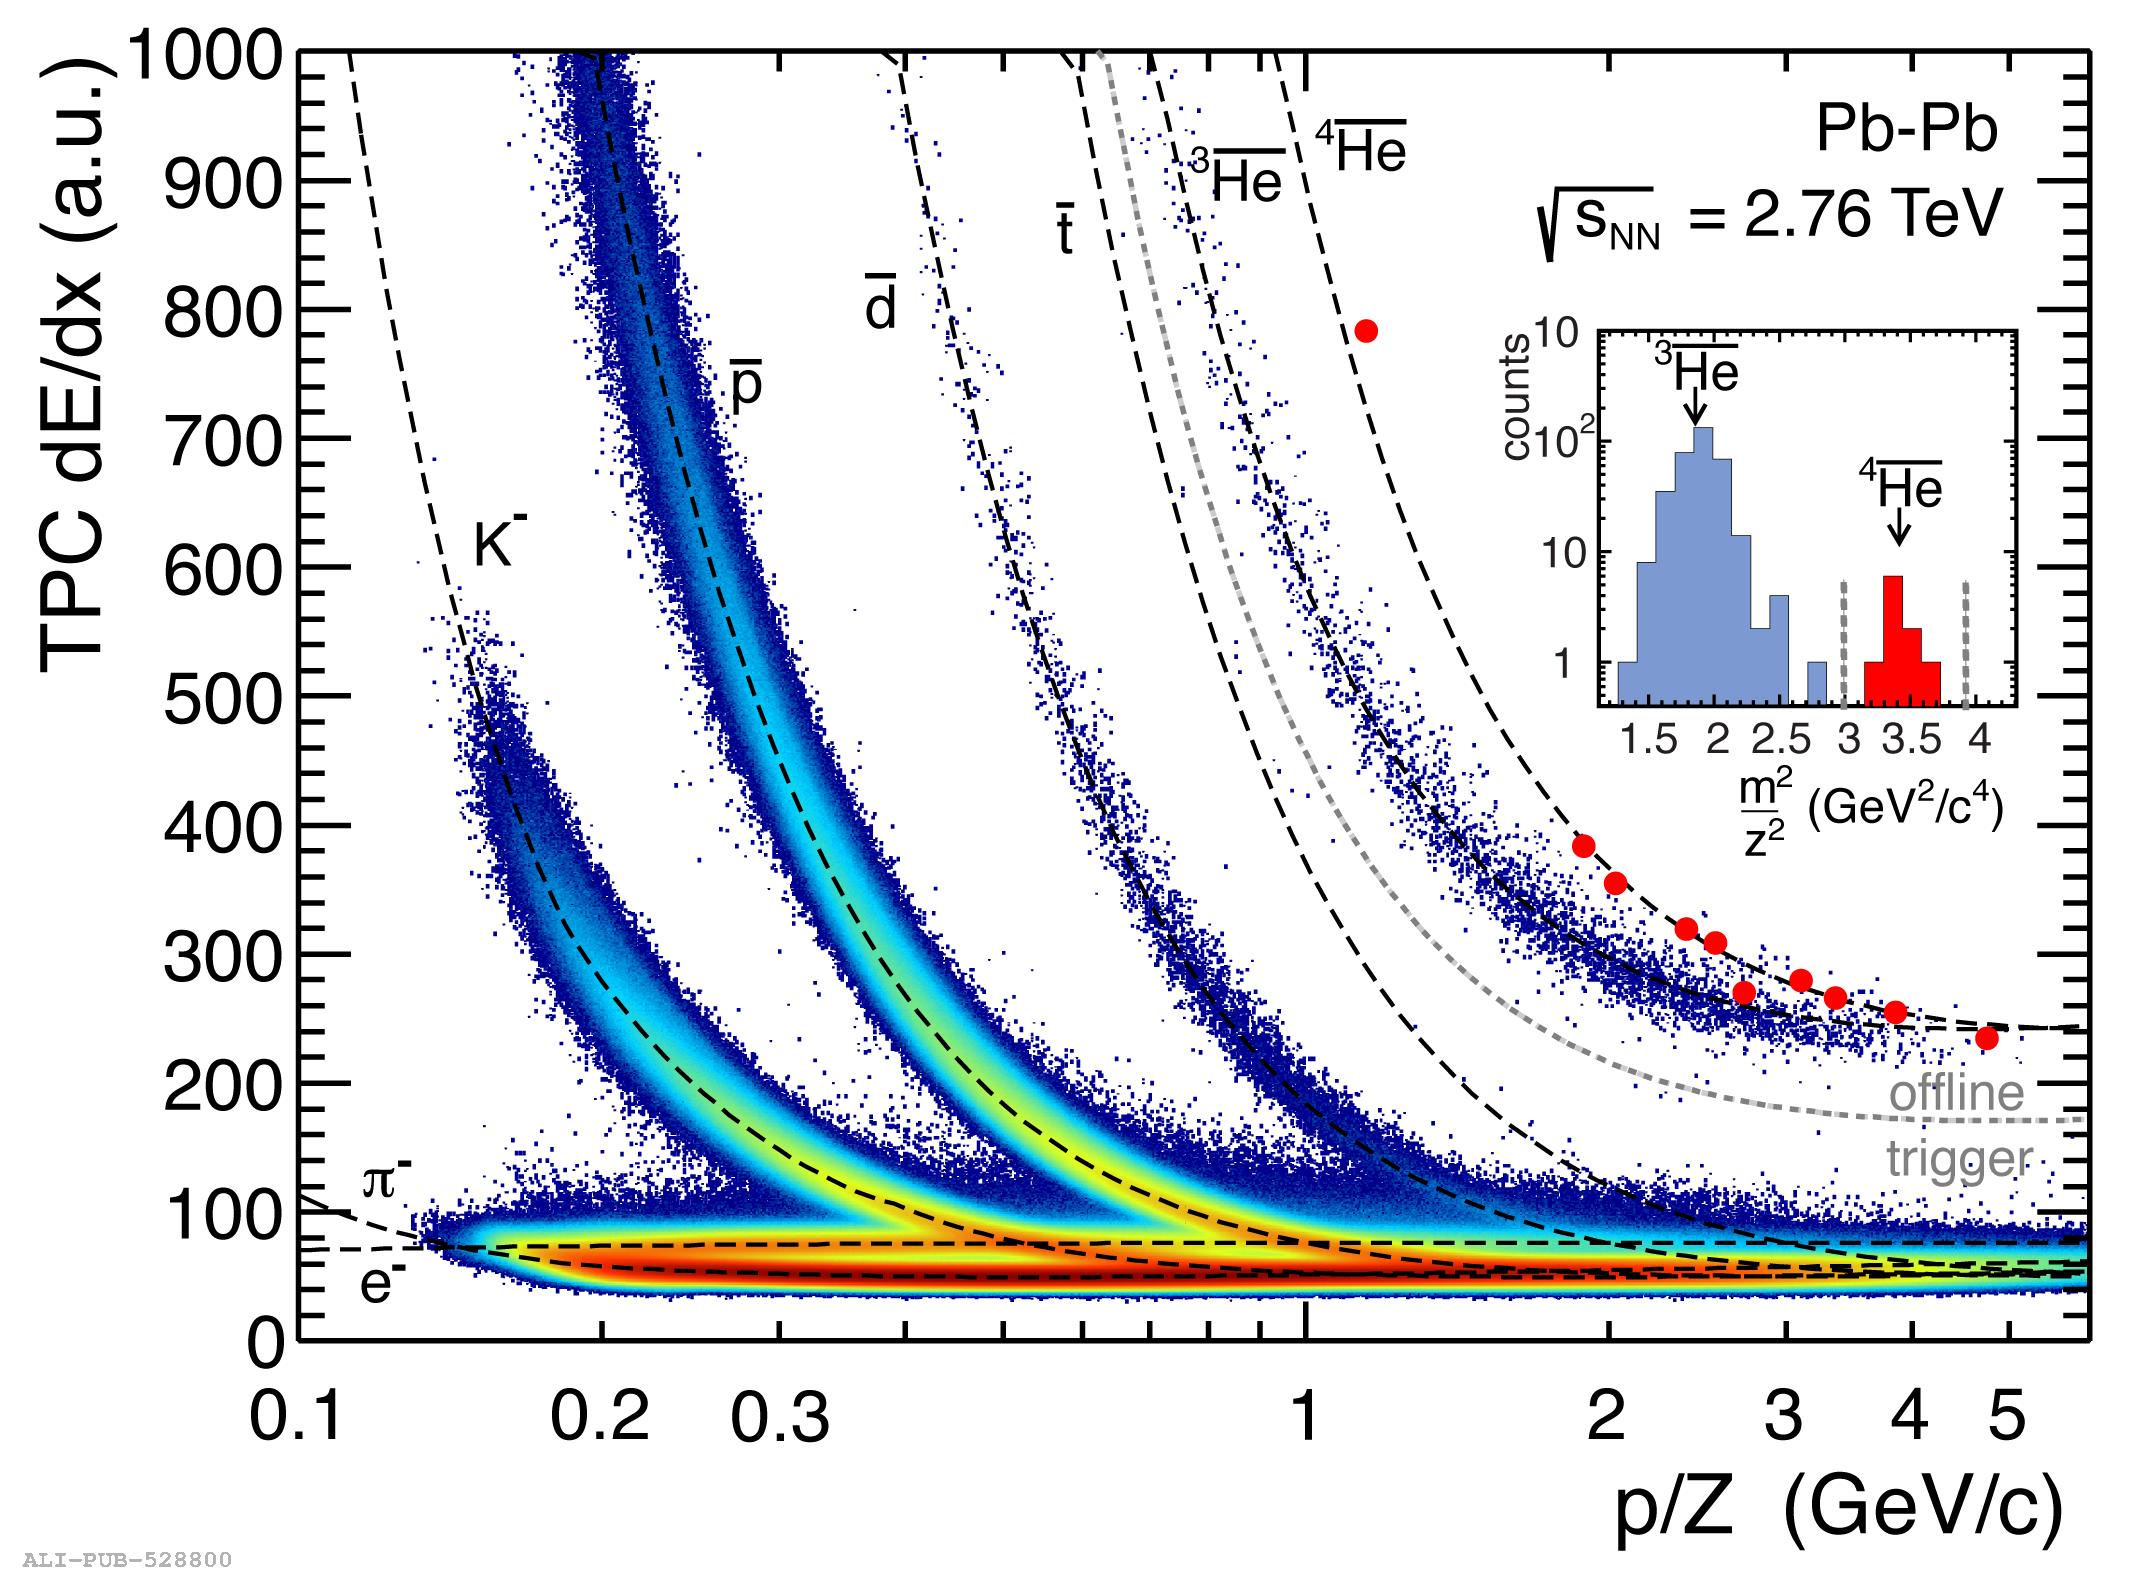
\includegraphics[width=0.8\textwidth]{Figs/Chapter3/dEdx_PbPb_2011_withAlphaInlet_NoLogo.eps}
%DIFDELCMD < 	%%%
%DIFDELCMD < \caption{%
{%DIFAUXCMD
\DIFdelFL{Energy deposition of various charged particles (electron, pion, kaon, anti-proton, anti-deuteron, anti-tritium, and two anti-helium isotopes) in the ALICE TPC in arbitrary units as a function of the magnetic rigidity (momentum over charge number). The dashed lines correspond to the theoretical expectations for each particle species. Figure taken from \mbox{%DIFAUXCMD
\cite{alicecollaborationALICEExperimentJourney2022}}\hspace{0pt}%DIFAUXCMD
.}}
	%DIFAUXCMD
%DIFDELCMD < \label{fig:TPCdEdx}
%DIFDELCMD < \end{figure}
%DIFDELCMD < 

%DIFDELCMD < %%%
\DIFdelend The spatial resolution varies from 1100 to 800 \mum in the transverse plane, and 1250 to 1100 \mum along the beam axis. Although the TPC can not compete with the \DIFdelbegin \DIFdel{level }\DIFdelend \DIFaddbegin \DIFadd{degree }\DIFaddend of precision of the ITS, it stands as the main tracking detector in ALICE thanks to its almost continuous sampling of the particle trajectory over large distances.

Moreover, the pad rows provides an analogue readout of the charge deposition, \DIFdelbegin \DIFdel{that }\DIFdelend \DIFaddbegin \DIFadd{which }\DIFaddend is used to measure the energy loss of charged particles per unit of length (\dEdx) with a resolution ($\sigma_{\rm TPC}$) ranging from \DIFdelbegin \DIFdel{5.5}\DIFdelend \DIFaddbegin \DIFadd{5.2}\DIFaddend \% in pp events to 6.5\% in the most central Pb-Pb collisions. As the energy deposition is stochastic phenomenon \DIFaddbegin \DIFadd{by nature}\DIFaddend , only the moments of its underlying distribution can be predicted. For instance, the Bethe-Bloch formula describes the mean \dEdx:
\DIFaddbegin 

\DIFaddend \begin{equation}
\begin{split}
\langle -\frac{dE}{dx} \rangle &= K z^{2} \frac{Z}{A} \frac{1}{\beta^{2}} \left[ \frac{1}{2} \ln \frac{2 m_{e} c^{2} \beta^{2} \gamma^{2} T_{\rm max}}{I} - \beta^{2} - \frac{\delta \left( \beta \gamma \right)}{2} \right],\\
\beta \gamma &= \frac{p}{M c}
\end{split}
\label{eq:BetheBloch}
\end{equation}
with 
\begin{itemize}
\item[$\bullet$] $Z$, the atomic number of the absorber (the TPC gas in this case),
\item[$\bullet$] $A$, the atomic mass of the absorber (g.mol$^{-1}$),
\item[$\bullet$] $m_{e}$, the electron mass,
\item[$\bullet$] $z$, charge number of the incident ionising particle,
\item[$\bullet$] $M$, mass of the incident ionising particle,
\item[$\bullet$] $p$, momentum of the incident ionising particle,
\item[$\bullet$] $\beta$, velocity of the incident ionising particle in units of $c$,
\item[$\bullet$] $\gamma$, Lorentz factor of the incident ionising particle,
\item[$\bullet$] $I$, mean excitation energy of the absorber,
\item[$\bullet$] $\delta \left( \beta \gamma \right)$, density effect correction due to the polarisation of the absorber,
\item[$\bullet$] $T_{\rm max} = \frac{2 m_{e} c^{2} \beta^{2} \gamma^{2}}{1 + 2 \gamma m_{e}/M + \left( m_{e}/M \right)^{2} }$, the maximum energy transfer to an electron in a single collision, 
\item[$\bullet$] $K$, \DIFdelbegin \DIFdel{a constant }\DIFdelend \DIFaddbegin \DIFadd{an independent constant of the ionising incident particle or the absorber}\DIFaddend .
\end{itemize}

As a matter of fact, the energy deposition follows a Landau distribution. Its broad tail on the high-energy-loss side leads the mean energy loss to be \DIFdelbegin \DIFdel{considerably }\DIFdelend \DIFaddbegin \DIFadd{significantly }\DIFaddend greater than the most probable value. \DIFdelbegin \DIFdel{It turns out that }\DIFdelend \DIFaddbegin \DIFadd{However, }\DIFaddend the most probable energy loss is much easier to evaluate than the mean \DIFdelbegin \DIFdel{, requiring }\DIFdelend \DIFaddbegin \DIFadd{that requires }\DIFaddend large samples to converge. Thereby, the Landau distribution is usually truncated \DIFdelbegin \DIFdel{only to keep }\DIFdelend \DIFaddbegin \DIFadd{to keep only }\DIFaddend the 50 to 70\% smallest values, and by so doing, the truncated mean coincides with the most probable energy loss \cite{particledatagroupReviewParticlePhysics2022}.\\


\Fig\ref{fig:TPCdEdx} shows clearly the characteristic \dEdx bands associated to \electron, \rmPi, \proton, \rmDeuton, \rmTriton, \rmHeThree and \rmHeFour. The measurements distribute around dashed lines, that correspond to the expected mean value given by the Bethe-Bloch formula (\eq\ref{eq:BetheBloch}). By comparing the measured value to the expected energy loss for various particle species, the nature of the incident particle can be determined. The PID estimator\DIFaddbegin \DIFadd{,
}\DIFaddend \begin{equation}
n_{\sigma} = \frac{ \langle \dEdx \rangle_{\rm meas} - \langle \dEdx \rangle_{\rm exp, i}}{\sigma_{\rm TPC}}\DIFaddbegin \DIFadd{,
}\DIFaddend \end{equation}
gives the distance between measured \dEdx and the expected one under the particle mass hypothesis $m_{\rm i}$ (i $=$ \electron, \rmPi, \proton, \rmDeuton, \rmTriton, \rmHeThree, \rmHeFour), in units of relative resolution $\sigma_{\rm TPC}$. \DIFdelbegin \DIFdel{So}\DIFdelend \DIFaddbegin \DIFadd{Therefore}\DIFaddend , the TPC \DIFdelbegin \DIFdel{can }\DIFdelend \DIFaddbegin \DIFadd{is able to }\DIFaddend distinguish a pion/electron from a kaon with a separation power better than 3$\sigma$ below $\sim$ 300 \mmom, and a kaon from a proton up to 1 \gmom.

\DIFdelbegin %DIFDELCMD < \begin{figure}[b]
%DIFDELCMD < %%%
\DIFdelendFL \DIFaddbeginFL \begin{figure}[t]
	\centering
	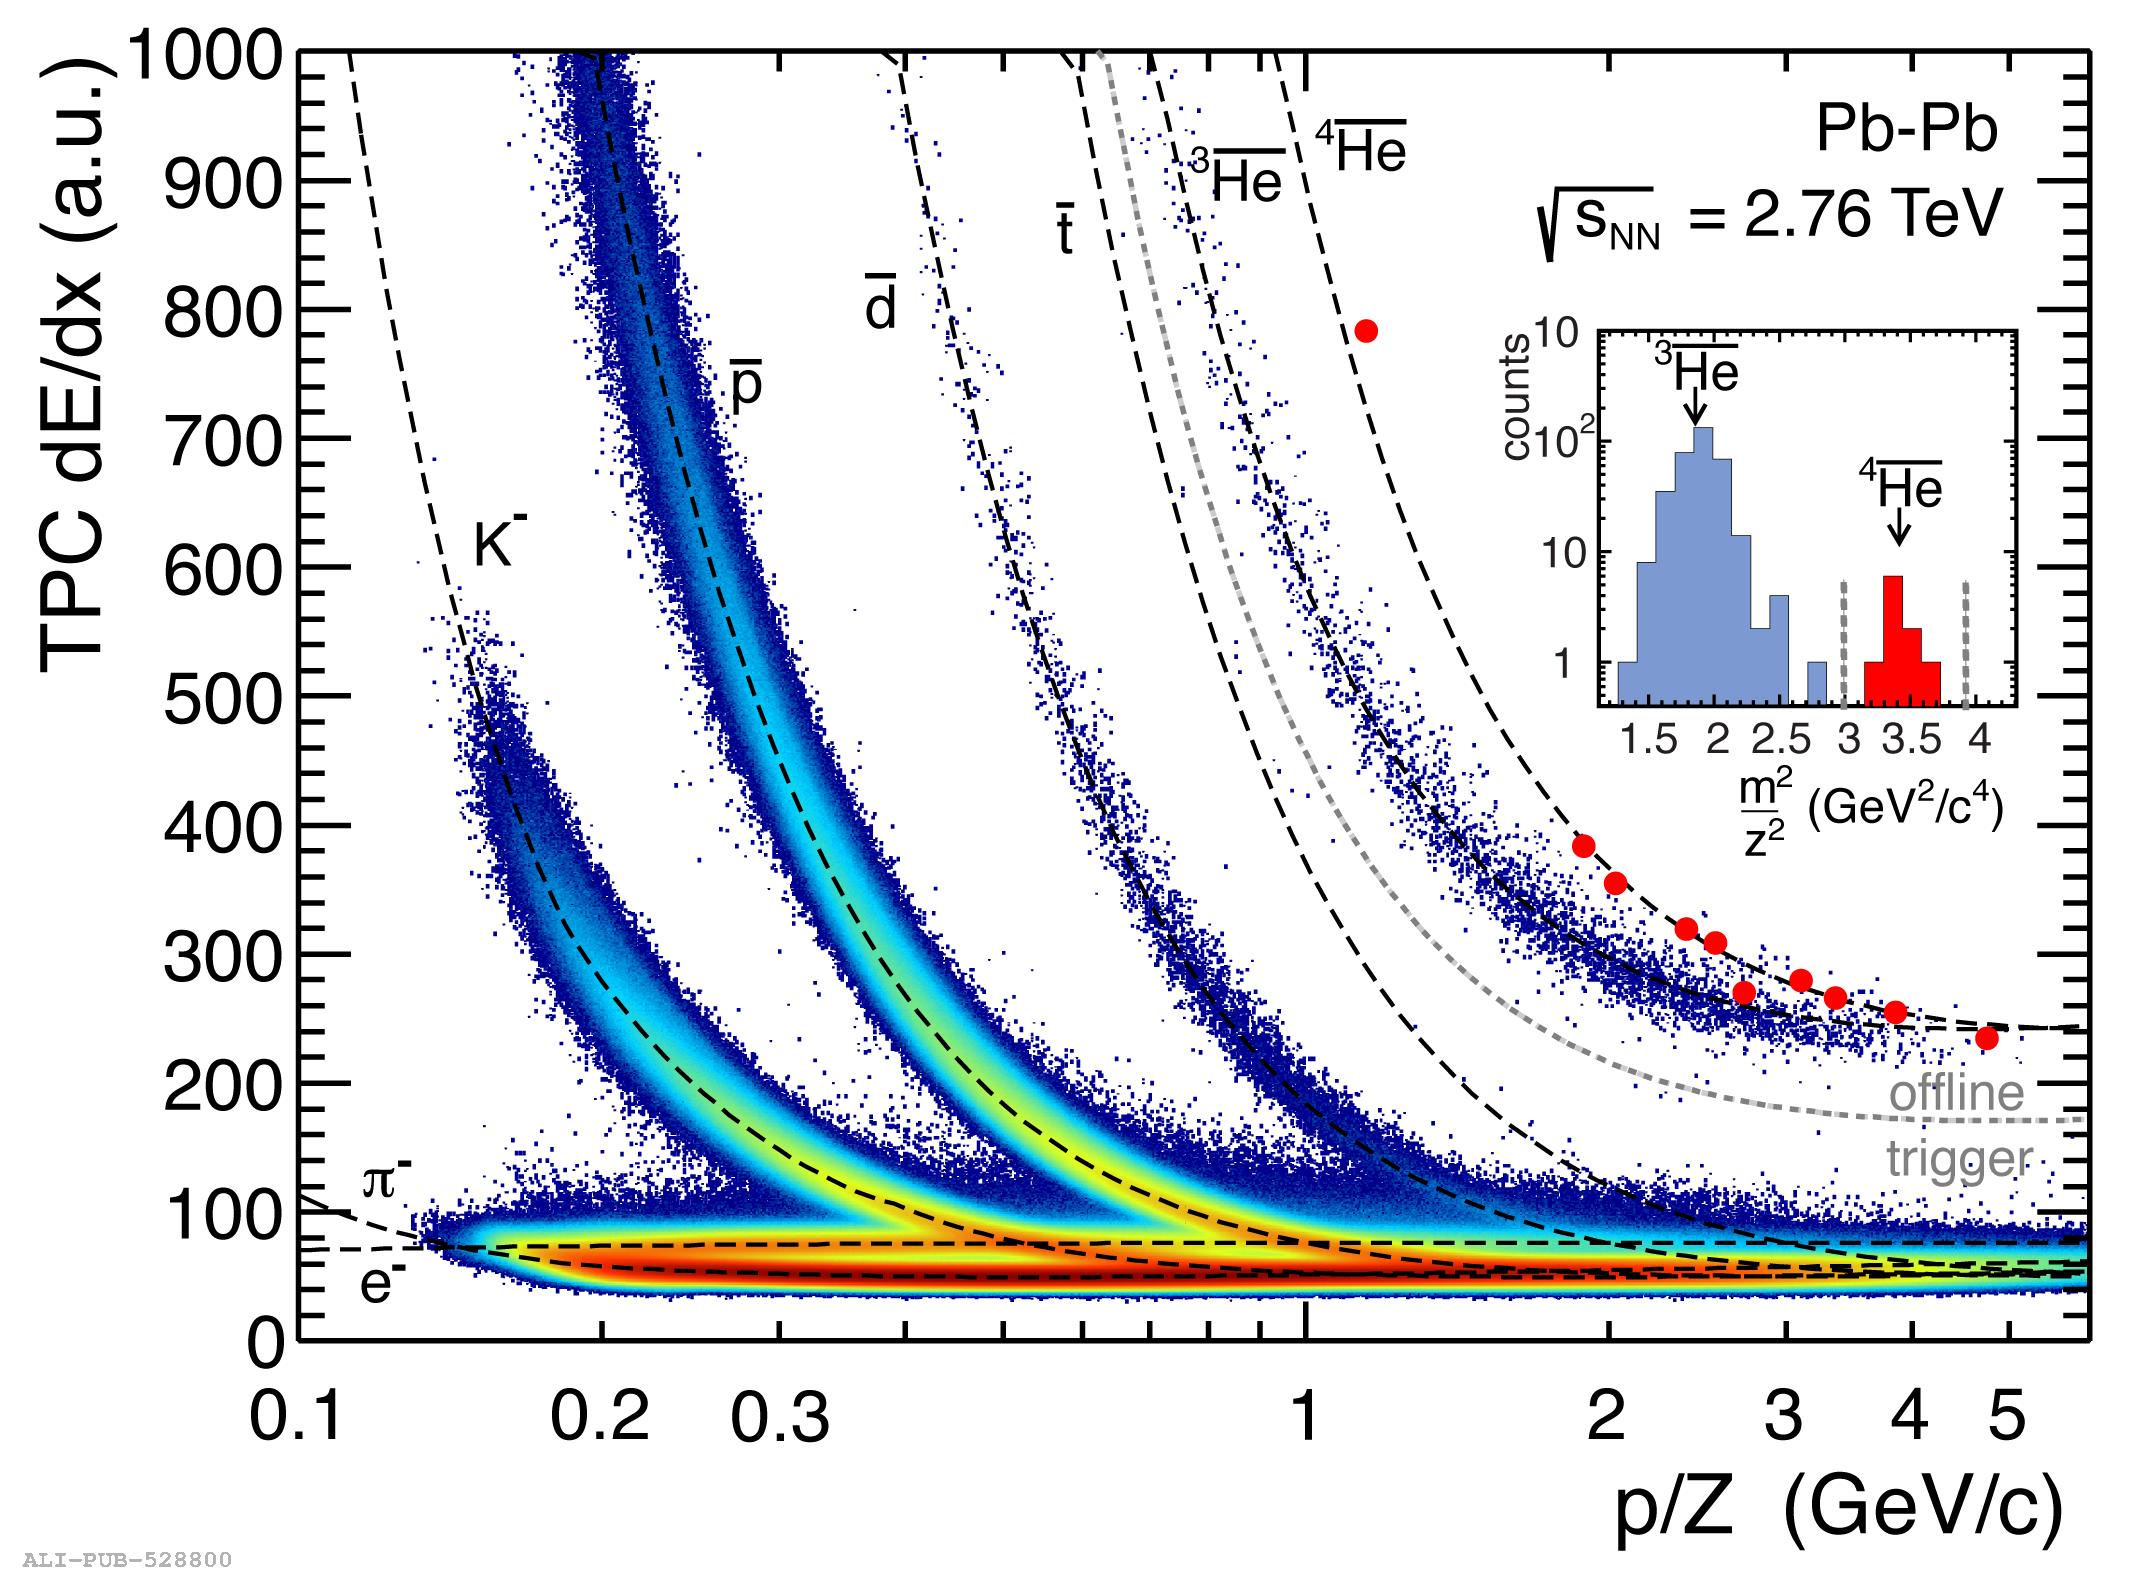
\includegraphics[width=0.8\textwidth]{Figs/Chapter3/dEdx_PbPb_2011_withAlphaInlet_NoLogo.eps}
	\caption{\DIFaddFL{Energy deposition of various charged particles (electron, pion, kaon, anti-proton, anti-deuteron, anti-tritium, and two anti-helium isotopes) in the ALICE TPC in arbitrary units as a function of the magnetic rigidity (momentum over charge number). The dashed lines correspond to the theoretical expectations for each particle species. Figure taken from \mbox{%DIFAUXCMD
\cite{alicecollaborationALICEExperimentJourney2022}}\hspace{0pt}%DIFAUXCMD
.}}
	\label{fig:TPCdEdx}
\end{figure}


\subsubsection{\DIFadd{VZERO}}
\label{subsubsec:VZERO}

\begin{figure}[t]
\DIFaddendFL \centering
\subfigure[]
{
	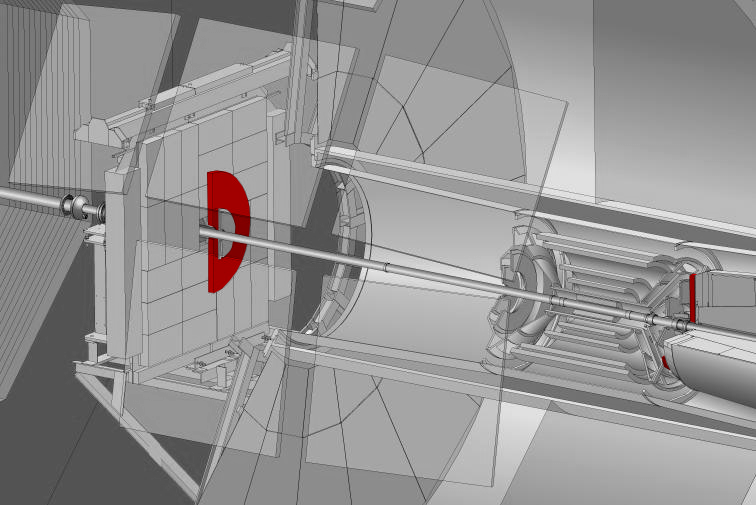
\includegraphics[width=0.6\textwidth]{Figs/Chapter3/ALICE-3D-Run1+2-ITS+V0-Inlay-v0-2012-08-02-Highlight-VZERO.png}
	\label{fig:VZEROinALICE}
}	
\subfigure[]
{
	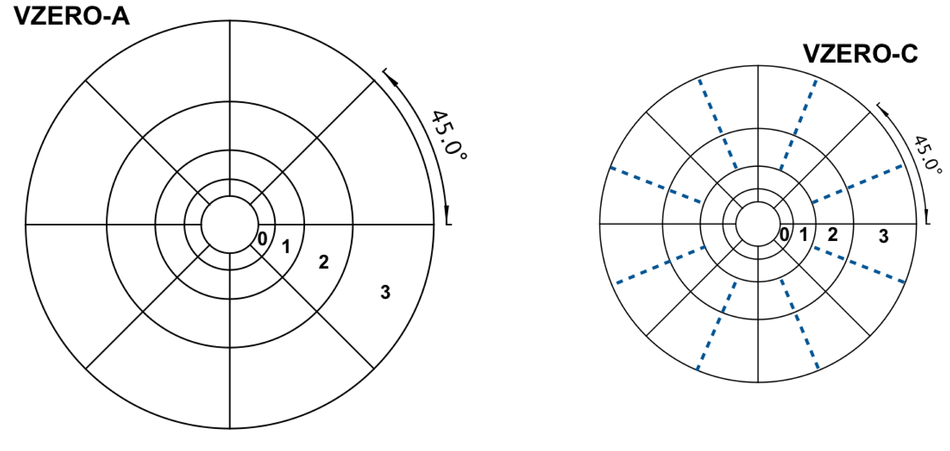
\includegraphics[width=0.8\textwidth]{Figs/Chapter3/Fig1-4206.png}
	\label{fig:VZEROarrays}
}
	\caption{(Top panel) View of the VZERO scintillator arrays inside the ALICE apparatus: VZERO-A on the left, and VZERO-C on the right. (Bottom panel) Sketches of the VZERO-A (left) and VZERO-C (right) with their segmentation. The dashed lines delimit segments connected to the same photomultiplier tube. Figures taken from \cite{alicecollaborationALICEExperimentJourney2022}\cite{alicecollaborationPerformanceALICEVZERO2013}.}
	\label{fig:VZEROdetector}
\end{figure}

\DIFdelbegin \subsubsection{\DIFdel{VZERO}}
%DIFAUXCMD
\addtocounter{subsubsection}{-1}%DIFAUXCMD
%DIFDELCMD < \label{subsubsec:VZERO}
%DIFDELCMD < 

%DIFDELCMD < %%%
\DIFdelend The VZERO system consists in two scintillator arrays, VZERO-A and VZERO-C, covering the pseudo-rapidity ranges $2.8 < \eta < 5.1$ and $-3.7 < \eta < -1.7$ respectively (\fig\ref{fig:VZEROinALICE}). It plays a crucial role in the data taking of ALICE as it provides minimum-bias triggers for the experiment, measures the charged particle multiplicity and centrality, and participates in the beam luminosity determination.


Each \DIFdelbegin \DIFdel{of }\DIFdelend array is segmented in four rings, themselves being divided in eight sections\DIFdelbegin \DIFdel{of }\DIFdelend \DIFaddbegin \DIFadd{, for a total of 32 cells made of }\DIFaddend 45\DIFdelbegin \DIFdel{wide made of }\DIFdelend \DIFaddbegin \DIFadd{\textdegree$\ $ wide }\DIFaddend plastic scintillators, as sketched in the \fig\ref{fig:VZEROarrays}. Because of the integration constraints (mainly coming from the muon absorber), \DIFdelbegin \DIFdel{two arrays needed to be designed}\DIFdelend \DIFaddbegin \DIFadd{the arrays come in two different designs}\DIFaddend . The 2.5 \cm thick VZERO-A sits at \DIFdelbegin \DIFdel{329 }\DIFdelend \DIFaddbegin \DIFadd{$z = 329$ }\DIFaddend \cm from the \DIFdelbegin \DIFdel{nominal vertex }\DIFdelend \DIFaddbegin \DIFadd{origin of the detector }\DIFaddend ($z = 0$). Since the VZERO-C stands in front of the muon absorber, the scintillator thickness \DIFdelbegin \DIFdel{reduces }\DIFdelend \DIFaddbegin \DIFadd{has been reduced }\DIFaddend to 2 \cm and its rings are positionned between -86 and -88 \cm along the beam axis. 

\DIFdelbegin %DIFDELCMD < \begin{figure}[h]
%DIFDELCMD < 	\centering
%DIFDELCMD < 	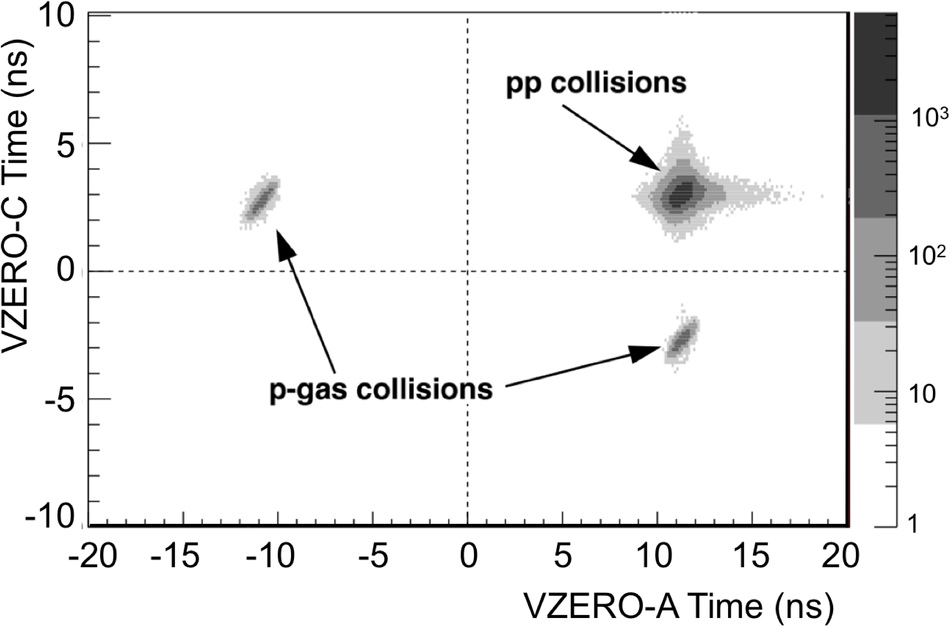
\includegraphics[width=0.8\textwidth]{Figs/Chapter3/Fig6_2-4228.png}
%DIFDELCMD < 	%%%
%DIFDELCMD < \caption{%
{%DIFAUXCMD
\DIFdelFL{Time of flight of the particles detected in the VZERO-C versus VZERO-A. Figure taken from \mbox{%DIFAUXCMD
\cite{alicecollaborationPerformanceALICEVZERO2013}}\hspace{0pt}%DIFAUXCMD
.}}
	%DIFAUXCMD
%DIFDELCMD < \label{fig:VZERObeamgas}
%DIFDELCMD < \end{figure}
%DIFDELCMD < 

%DIFDELCMD < %%%
\DIFdelend The passage of a charged particle in the scintillator generates light, that is guided to photomultiplier tubes via 1 \mm in diameter Wave-Length Shifting and optical fibers. For each of the 32 elementary cells, the photomultiplier tube outputs two analogue signals. The first measures the integrated charge, the second -- amplified by a factor 10 -- determines the pulse/arrival time relative to the LHC bunch clock with a resolution better than 1 \nsec. Each signal gives rise to a specific type of trigger algorithm. 

Based on the coincidence between the time signals from the arrays, beam-induced background events\footnote{They typically correspond to beam-gas collisions, that is a collision between a bunch from the beam and a residual \DIFdelbegin \DIFdel{atom }\DIFdelend \DIFaddbegin \DIFadd{gas molecule }\DIFaddend in the beam pipe} can be rejected. \Fig\ref{fig:VZERObeamgas} shows an example of such rejection. A particle coming from the interaction point takes about 11 \nsec and 3 \nsec to reach the VZERO-A and the VZERO-C respectively. If the \DIFdelbegin \DIFdel{time of flight of the particles detected in the two }\DIFdelend \DIFaddbegin \DIFadd{signals mesured in the both }\DIFaddend scintillator arrays matches these values --- as \DIFdelbegin \DIFdel{it is the case }\DIFdelend in the top right corner of \fig\ref{fig:VZERObeamgas} ---, this \DIFdelbegin \DIFdel{would indicate }\DIFdelend \DIFaddbegin \DIFadd{indicates }\DIFaddend that a beam-beam collision \DIFaddbegin \DIFadd{have }\DIFaddend occured. However, the signals arriving in coincidence at -12 \nsec (VZERO-A) and 3 \nsec (VZERO-C), and 11 \nsec (VZERO-A) and -3 \nsec (VZERO-C) are not the signatures of a beam-beam event. They correspond to beam-gas collisions coming from the A-side and C-side respectively. This is the first type of trigger algorithm.

\DIFaddbegin \begin{figure}[t]
	\centering
	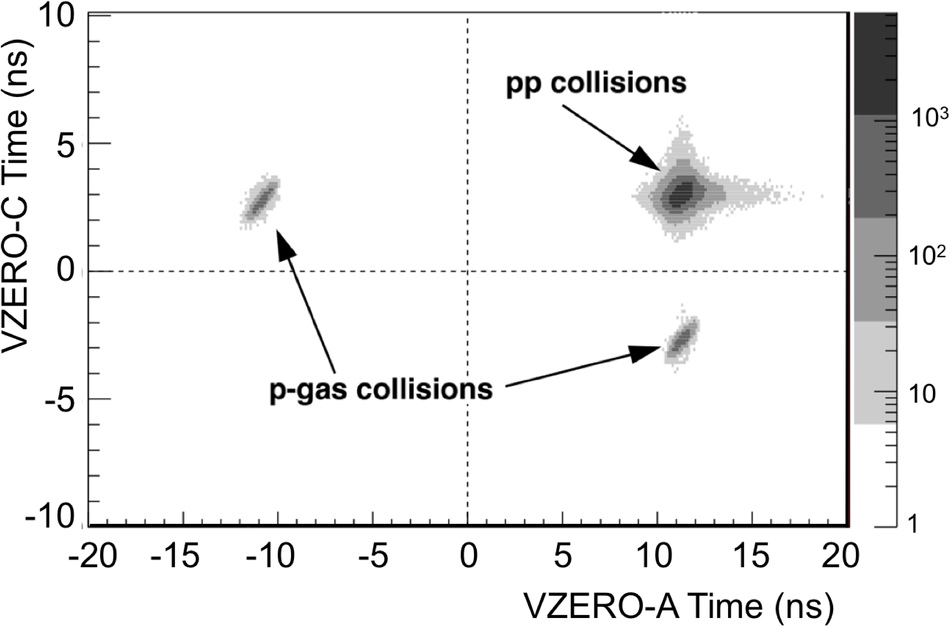
\includegraphics[width=0.8\textwidth]{Figs/Chapter3/Fig6_2-4228.png}
	\caption{\DIFaddFL{Time of flight of the particles detected in the VZERO-C versus VZERO-A. Figure taken from \mbox{%DIFAUXCMD
\cite{alicecollaborationPerformanceALICEVZERO2013}}\hspace{0pt}%DIFAUXCMD
.}}
	\label{fig:VZERObeamgas}
\end{figure}

\begin{figure}[h]
	\centering
	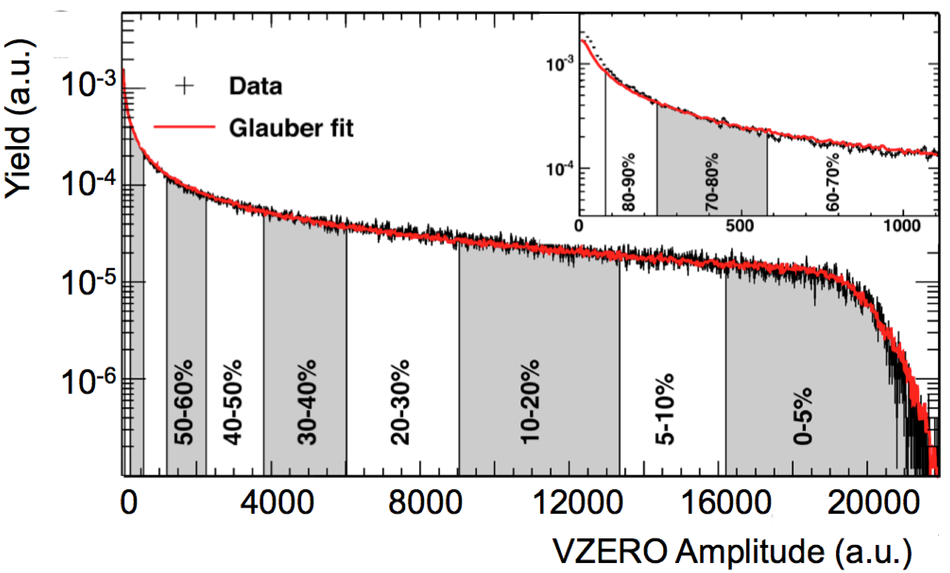
\includegraphics[width=0.8\textwidth]{Figs/Chapter3/Fig8-4236.png}
	\caption{\DIFaddFL{Total yield as a function of the signal amplitudes in the two VZERO arrays in Pb-Pb collisions at \sqrtSnn = 2.76 }\tev\DIFaddFL{, fitted with a Glauber model in red. The shaded areas correspond to different centrality classes. Figure taken from \mbox{%DIFAUXCMD
\cite{alicecollaborationPerformanceALICEVZERO2013}}\hspace{0pt}%DIFAUXCMD
.}}
	\label{fig:VZEROcentrality}
\end{figure}

\DIFaddend The energy deposited in the scintillators provides a measurement of the charged particle multiplicity. Based on a simulation of \DIFaddbegin \DIFadd{the }\DIFaddend VZERO detectors, the total charge collected can be related to the number of primary charged particles\DIFdelbegin \DIFdel{. \Fig\ref{fig:VZEROcentrality}shows the relation between these two quantities}\DIFdelend \DIFaddbegin \DIFadd{, as shown in \fig\ref{fig:VZEROcentrality}}\DIFaddend . The second type of trigger algorithm consists in dividing the distribution of the V0 amplitudes in different multiplicity/centrality\footnote{In heavy-ion collisions, \DIFdelbegin \DIFdel{as in \fig\ref{fig:VZEROcentrality}, }\DIFdelend the impact parameter -- and, \textit{a fortiori}, its percentage value, the centrality -- \DIFdelbegin \DIFdel{can not }\DIFdelend \DIFaddbegin \DIFadd{cannot }\DIFaddend be measured directly\DIFdelbegin \DIFdel{. However}\DIFdelend , \DIFdelbegin \DIFdel{since }\DIFdelend \DIFaddbegin \DIFadd{but the number of charged particle is measurable using -- among others -- the VZERO detectors. Since }\DIFaddend the centrality and the charged particle multiplicity in the event are correlated\DIFaddbegin \DIFadd{, the latter allows to recover the centrality }\DIFaddend (\DIFaddbegin \DIFadd{as }\DIFaddend confirmed by \DIFaddbegin \DIFadd{the }\DIFaddend Glauber fit \DIFaddbegin \DIFadd{in \fig\ref{fig:VZEROcentrality}}\DIFaddend , that \DIFaddbegin \DIFadd{also }\DIFaddend gives access to the centrality)\DIFaddbegin \DIFadd{. Hence, for heavy-ion collisions}\DIFaddend , the different intervals in multiplicity \DIFaddbegin \DIFadd{in \fig\ref{fig:VZEROcentrality} }\DIFaddend are \DIFdelbegin \DIFdel{refered }\DIFdelend \DIFaddbegin \DIFadd{referred }\DIFaddend as \textit{centrality classes}.} classes from the 5\%-highest multiplicity to the 10\%-lowest multiplicity events, as represented in shaded areas. 

\DIFdelbegin %DIFDELCMD < \begin{figure}[h]
%DIFDELCMD < 	\centering
%DIFDELCMD < 	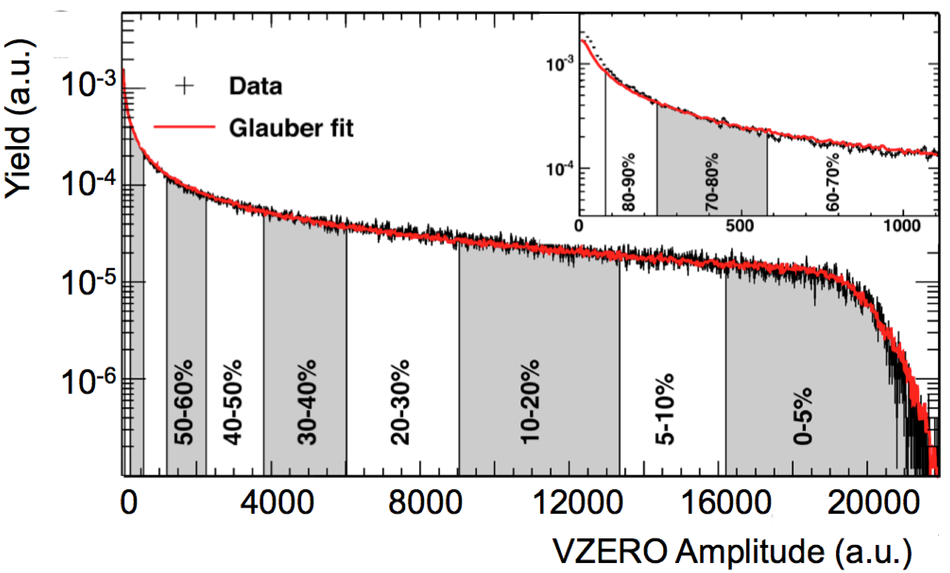
\includegraphics[width=0.8\textwidth]{Figs/Chapter3/Fig8-4236.png}
%DIFDELCMD < 	%%%
%DIFDELCMD < \caption{%
{%DIFAUXCMD
\DIFdelFL{Total yield as a function of the signal amplitudes of the two VZERO arrays in Pb-Pb collisions at \sqrtSnn = 2.76 }%DIFDELCMD < \tev%%%
\DIFdelFL{, fitted with a Glauber model in red. The shaded areas correspond to different centrality classes. Figure taken from \mbox{%DIFAUXCMD
\cite{alicecollaborationPerformanceALICEVZERO2013}}\hspace{0pt}%DIFAUXCMD
.}}
	%DIFAUXCMD
%DIFDELCMD < \label{fig:VZEROcentrality}
%DIFDELCMD < \end{figure}
%DIFDELCMD < 

%DIFDELCMD < %%%
\DIFdelend \subsubsection{Time-Of-Flight detector}
\label{subsubsec:TOF}

The Time-Of-Flight (TOF) detector is a large cylindrical array with an inner radius of 370 \cm and an outer one of 399 \cm. It covers the central pseudo-rapidity region, that is $|\eta| < 0.9$, and the full azimuth. While the separation power of TPC only goes up to 1 \gmom, the TOF detector aims at providing particle identification at intermediate momentum from 0.2 to 2.5 \gmom.  To instrument this large volume (17.5 $\m^{3}$), a gaseous detector is employed, as its manufacture \DIFdelbegin \DIFdel{remains rather }\DIFdelend \DIFaddbegin \DIFadd{turns out to be relatively }\DIFaddend simple and thus \DIFaddbegin \DIFadd{quite }\DIFaddend inexpensive. The best solution, with respect to the design considerations of the experiment, is the Multi-gap Resistive-Plate Chamber (MRPC) \cite{akindinovMultigapResistivePlate2000}. 

The basic constituent of the TOF system is a pair of MRPC strips, 122 \cm in length and 12 \cm in width, stacked together with an active area of 120 $\times$ 7.4 $\cm^{2}$. As shown in \fig\ref{fig:TOFMRPC}, it consists in two cathodes and a central anode \DIFdelbegin \DIFdel{placed }\DIFdelend in a gas volume\DIFaddbegin \DIFadd{, }\DIFaddend and spaced by five 0.4 \mm thin glass plates (with a 250 \mum gap) for each strip. The full volume is filled with a gas mixture composed of C$_{2}$H$_{2}$F$_{4}$(90\%), C$_{4}$H$_{10}$(5\%), SF$_{6}$(5\%), as it shows no ageing effects and  has a rate capability much higher than the expected \DIFdelbegin \DIFdel{one }\DIFdelend \DIFaddbegin \DIFadd{rate }\DIFaddend in ALICE \cite{akindinovStudyGasMixtures2004}.

\DIFdelbegin %DIFDELCMD < \begin{figure}[t]
%DIFDELCMD < %%%
\DIFdelFL{\hspace*{-1.5cm}
}%DIFDELCMD < \subfigure[]
%DIFDELCMD < {
%DIFDELCMD < 	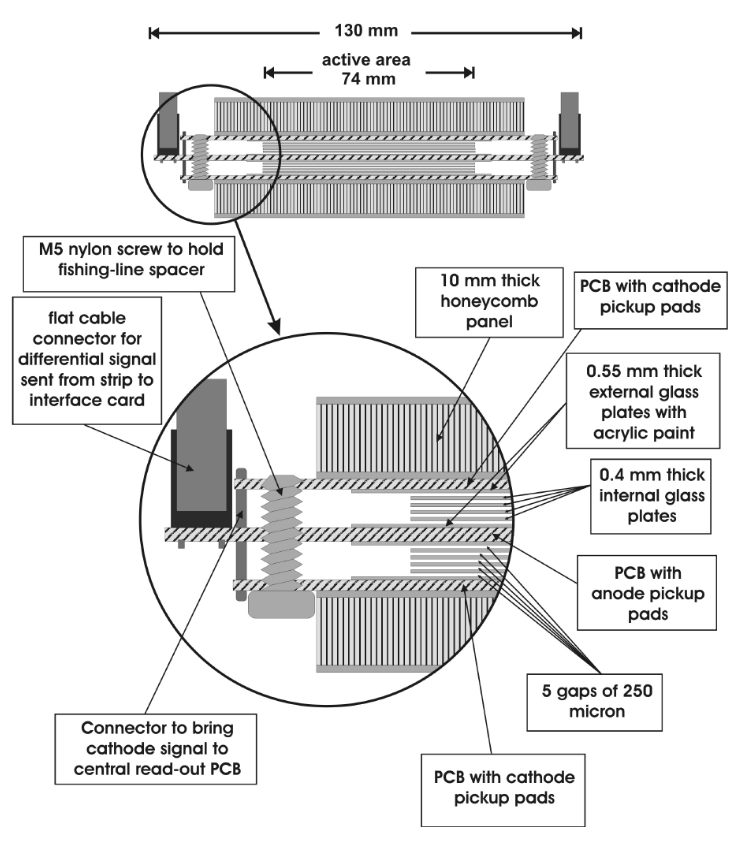
\includegraphics[width=0.5\textwidth]{Figs/Chapter3/TOFMRPC.png}
%DIFDELCMD < 	\label{fig:TOFMRPC}
%DIFDELCMD < }
%DIFDELCMD < \subfigure[]
%DIFDELCMD < {
%DIFDELCMD < 	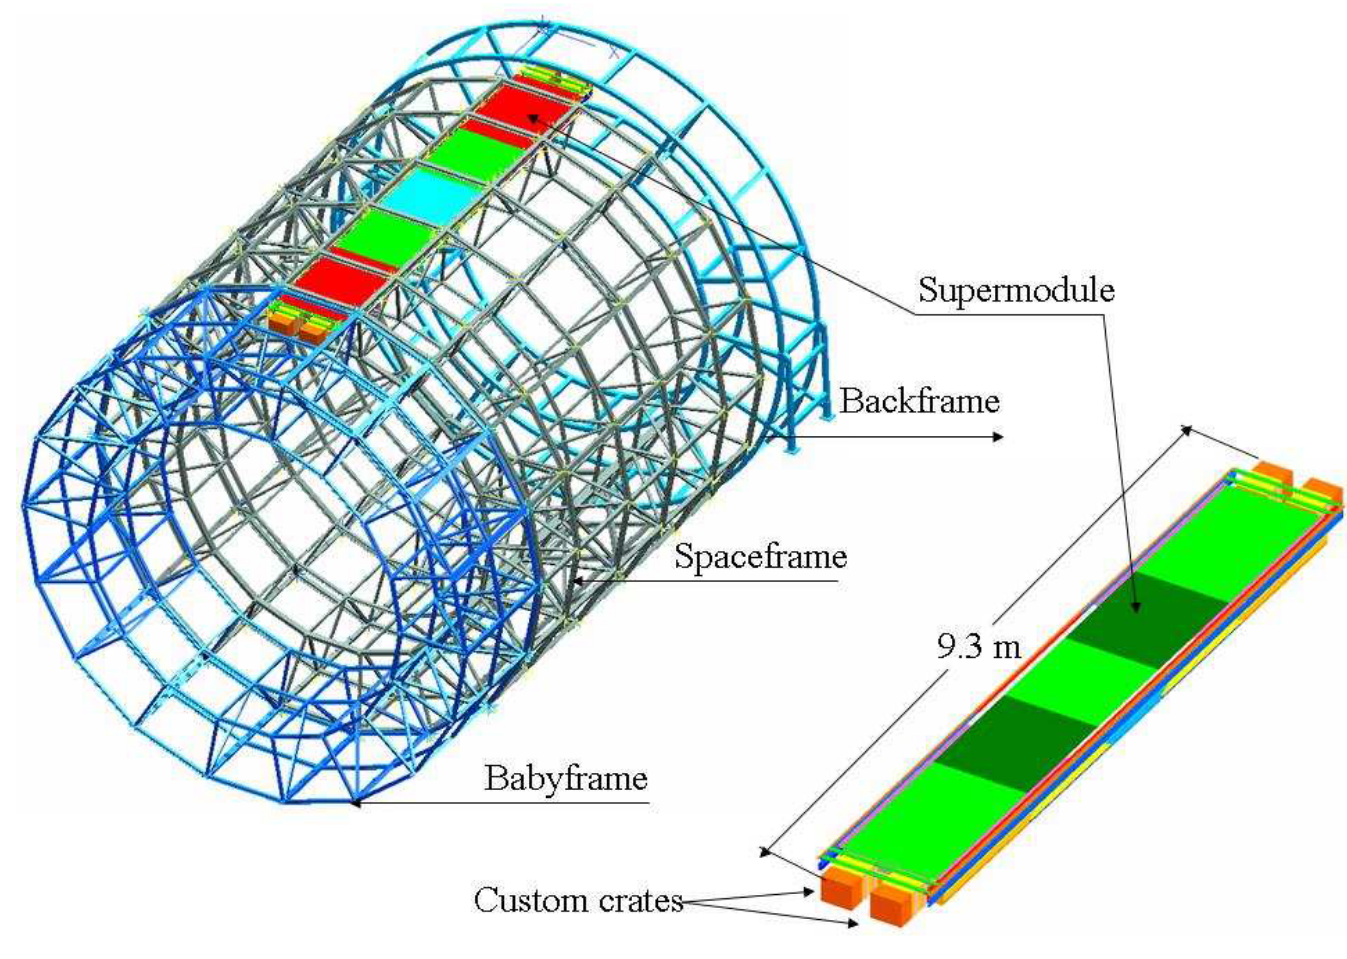
\includegraphics[width=0.75\textwidth]{Figs/Chapter3/TOFSuperModule.png}
%DIFDELCMD < 	\label{fig:TOFStructure}
%DIFDELCMD < }	
%DIFDELCMD < 	%%%
%DIFDELCMD < \caption{%
{%DIFAUXCMD
\DIFdelFL{(Left panel) Drawing of the cross section of a 10-gap double-stack MRPC. (Right panel) Schematic view of the TOF barrel with one supermodule, consisting of five modules. Figure taken from \mbox{%DIFAUXCMD
\cite{alicecollaborationALICEExperimentCERN2008}}\hspace{0pt}%DIFAUXCMD
.}}
	%DIFAUXCMD
%DIFDELCMD < \label{fig:TOFPID}
%DIFDELCMD < \end{figure}
%DIFDELCMD < 

%DIFDELCMD < %%%
\DIFdelend To cover the full cylinder along the beam direction and minimise the cumulative dead areas from the innermost to outermost detectors in ALICE, five modules of different lengths are combined. The central element utilizes 117 \cm long module, the intermediate ones 137 \cm, the external ones 177 \cm made of 15 MRPC strips for the central module and 19 for the others. Altogether, they form a supermodule of total length 930 \cm with an overall active region of 741 $\times$ 7.4 $\cm^{2}$, as shown on \fig\ref{fig:TOFStructure}. Each of the 18 azimuthal sectors of the TOF system has a supermodule.

When a charged particle traverses the active volume, it ionises the gas along its path and produces electrons that drift to one of the cathodes. The key aspect of the MRPC resides in the high voltage of the anode (-13 kV), which delivers a high and uniform electrostatic field. The latter is sufficiently strong to start an avalanche process\footnote{Let us consider a medium containing free electrons and in which a strong electrostatic field exists. If the latter is strong enough, it accelerates the electrons such that they will collide with other atoms in the medium, \DIFdelbegin \DIFdel{thereby }\DIFdelend \DIFaddbegin \DIFadd{thus }\DIFaddend ionising them and releasing additionnal electrons. These ones also get accelerated and collide with other atoms, releasing more electrons, and so on. This chain reaction is called an avalanche process.}, and thereby to give rise to a detectable signal. The avalanche stops when it reaches a glass plate, but the produced electrons continue to drift -- and to create avalanches in the gaseous medium along the way -- until they are collected by the 48 cathode pad readouts of 3.5 $\times$ 2.5 $\cm^{2}$ from each strip. \\

\DIFaddbegin \begin{figure}[t]
\DIFaddFL{\hspace*{-1.5cm}
}\subfigure[]
{
	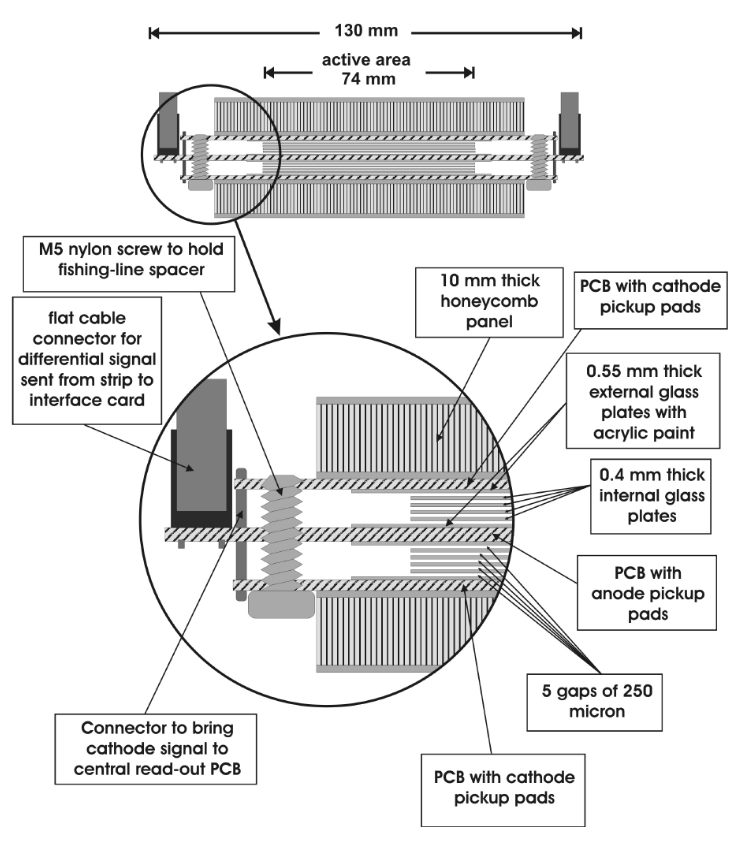
\includegraphics[width=0.5\textwidth]{Figs/Chapter3/TOFMRPC.png}
	\label{fig:TOFMRPC}
}
\subfigure[]
{
	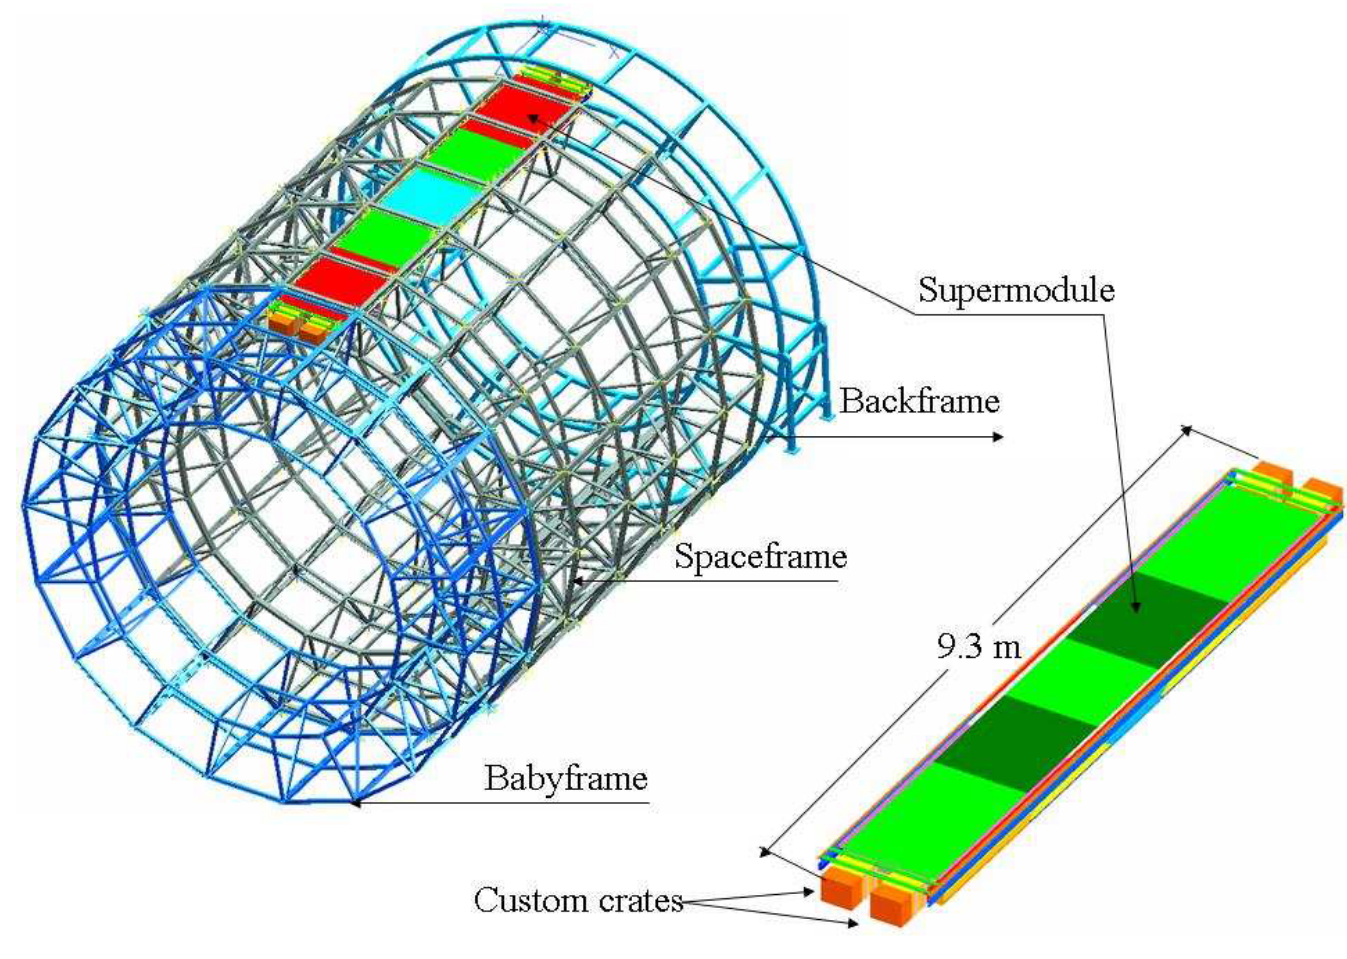
\includegraphics[width=0.75\textwidth]{Figs/Chapter3/TOFSuperModule.png}
	\label{fig:TOFStructure}
}	
	\caption{\DIFaddFL{(Left panel) Drawing of the cross section of a 10-gap double-stack MRPC. (Right panel) Schematic view of the TOF barrel with one supermodule, consisting of five modules. Figure taken from \mbox{%DIFAUXCMD
\cite{alicecollaborationALICEExperimentCERN2008}}\hspace{0pt}%DIFAUXCMD
.}}
	\label{fig:TOFPID}
\end{figure}

\DIFaddend Their output signals carry \DIFdelbegin \DIFdel{the information of }\DIFdelend \DIFaddbegin \DIFadd{informations on }\DIFaddend the deposited charge via the Time-Over-Threshold and the hit \DIFdelbegin \DIFdel{time -- }\DIFdelend \DIFaddbegin \DIFadd{times relative to the collision time, $t_{\rm ev}$ , }\DIFaddend with an intrinsic resolution of 56 \psec during the LHC Run-2\DIFdelbegin \DIFdel{-- relative to the collision time, $t_{\rm ev}$}\DIFdelend . Due to the finite size of the \DIFdelbegin \DIFdel{bunches that interact, the latter }\DIFdelend \DIFaddbegin \DIFadd{colliding bunches, $t_{\rm ev}$ }\DIFaddend has to be measured on an event-by-event basis. To that end, different options are available.

The most precise measurement of the collision time is provided by the T0 detector. It consists in two arrays, each made of twelve Cerenkov counters, placed at \DIFdelbegin \DIFdel{375 }\DIFdelend \DIFaddbegin \DIFadd{$z = 375$ }\cm \DIFaddend (T0-A) and -72.7 \cm (T0-C)\DIFdelbegin \DIFdel{from the nominal vertex}\DIFdelend . They respectively cover the pseudo-rapidity range $4.61 < \eta < 4.92 $ and $-3.28 < \eta < -2.97$. Each counter is a quartz radiator of 20 \mm in diameter and 20 \mm thick, connected optically to a PMT. The readout electronics is quite similar to the one used for the TOF detector, with a dead time below 25 \nsec. The T0 system gives two time measurements, \DIFdelbegin \DIFdel{$t_{\rm T0-A}$ and $t_{\rm T0-C}$, }\DIFdelend one for each array\DIFaddbegin \DIFadd{, $t_{\rm T0-A}$ and $t_{\rm T0-C}$}\DIFaddend . When both values are available, the average is taken as the start time of the event, $t_{\rm ev}^{\rm T0} = \left( t_{\rm T0-A} + t_{\rm T0-C} \right)/2$, with a resolution of 50 and 25 \psec in pp and Pb-Pb collisions. If only one of the two counters produces a signal, the collision time is given by either the $t_{\rm T0-A}$ or $t_{\rm T0-C}$ taking into account the longitudinal position of the primary vertex (provided by the ITS). Consequently, the resolution deteriorates to 100 and 60 \psec in pp collisions for the T0-A and \DIFdelbegin \DIFdel{-C }\DIFdelend \DIFaddbegin \DIFadd{T0-C }\DIFaddend respectively, and 50 and 30 \psec in heavy-ion collisions. Due to its limited acceptance, the triggering efficiency of the detector in coincidence is about 48\%, and reaches 60\% and 67\% for the T0-A and -C individually in pp collisions\footnote{The triggering efficiency is close to 100\% in heavy-ion collisions, due to \DIFdelbegin \DIFdel{the }\DIFdelend \DIFaddbegin \DIFadd{their inherently }\DIFaddend high multiplicities.}.

The TOF system itself can also determine $t_{\rm ev}$. Based on a sample of particles matching a hit in the detector, a $\chi^{2}$-minimisation procedure is performed in order to extract the set of mass hypotheses that minimises their combined time-of-flights. From this set derives the event collision time, denoted $t_{\rm ev}^{\rm TOF}$. By construction, this procedure only applies for a minimum number of two tracks, and the resolution improves with the track multiplicity (scaling as \DIFdelbegin \DIFdel{$\sim 1 / \sqrt{n_{\rm tracks}}$}\DIFdelend \DIFaddbegin \DIFadd{$\sim 1 / \sqrt{N_{\rm tracks}}$}\DIFaddend ). It allows to reach time resolution from 80 \psec for the low multiplicity events to 20 \psec for the high multiplicity events, with efficiencies ranging from 20\% to 100\% respectively.

Considering the above efficiencies, the collision start time can be obtained from the T0 or TOF measurement ($t_{\rm ev}^{\rm T0}$ or $t_{\rm ev}^{\rm TOF}$)\DIFdelbegin \DIFdel{or their combination, }\DIFdelend \DIFaddbegin \DIFadd{, or even their combination }\DIFaddend if both are available. In the latter case, the final $t_{\rm ev}$ corresponds to their weighted average, with the inverse of their resolution squared as weighting factors. If none of the preceding procedures is usable, the \DIFdelbegin \DIFdel{event time }\DIFdelend \DIFaddbegin \DIFadd{start time of the event }\DIFaddend is set on the LHC clock\footnote{In fact, it is set on zero as, after alignement and calibration of the TOF detector, the LHC clock phase has been shifted to coincide with the nominal starting time.} which has a resolution of 200 \psec \cite{alicecollaborationDeterminationEventCollision2017}.\\



\DIFdelbegin \DIFdel{Hence}\DIFdelend \DIFaddbegin \DIFadd{In any case}\DIFaddend , the difference between the arrival time $t_{\rm TOF}$ and the moment of the collision $t_{\rm ev}$ gives the \textit{measured time-of-flight} of the charged particle from the primary vertex to the TOF detector. \DIFdelbegin \DIFdel{Knowing the latter as well as the the distance travelled}\DIFdelend \DIFaddbegin \DIFadd{Based on the latter and the flight path length}\DIFaddend , the velocity of the particle -- or rather the ratio of the velocity to the speed of light, $\beta = v /c$ -- can be evaluated. The \fig\ref{fig:TOFPID} shows the distribution of $\beta$ \DIFdelbegin \DIFdel{of }\DIFdelend \DIFaddbegin \DIFadd{for }\DIFaddend charged particles measured by the TOF detector as a function of their momentum in Pb-Pb events at \sqrtSnn = 5.02 \tev. A clear separation of the electron, pion, kaon, proton and deuteron bands is visible. This stems from the relation between the particle mass $m$, its momentum $p$ and its velocity $\beta$: 
\begin{align}
m = \frac{p}{\beta \gamma} = p \ \sqrt{ \frac{1}{\beta^{2}} - 1 }& \qquad \textrm{with} \quad \beta = \frac{v}{c} = \frac{L}{c t_{\rm exp}},\\
\Rightarrow t_{\textrm{exp}} &= L \ \frac{\sqrt{p^{2} + m^{2}}}{c p}.
\label{eq:tTOF}
\end{align}

\begin{figure}[t]
	\centering
	\DIFdelbeginFL %DIFDELCMD < \includegraphics[width=0.8\textwidth]{Figs/Chapter3/TOFBetawoMismatchEtaCut_PbPb.eps}
%DIFDELCMD < 	%%%
\DIFdelendFL \DIFaddbeginFL \includegraphics[width=0.8\textwidth]{Figs/Chapter3/TOFBetawoMismatchEtaCut_PbPb.png}
	\DIFaddendFL \caption{Velocity ($\beta = v /c$) of electrons, pions, kaons, protons and deuterons as a function of their momentum (provided by the TPC), measured by the TOF detector, in Pb-Pb collisions at \sqrtSnn = 5.02 \tev. Figure taken from \cite{alicecollaborationALICEExperimentJourney2022}.}
	\label{fig:TOFPID}
\end{figure}

In \eq\ref{eq:tTOF}, $t_{\textrm{exp}}$ corresponds to the \textit{expected time-of-flight}, \ie the time it would take for a particle of mass $m$, with a momentum $p$, to go from the interaction point to the TOF detector following a path of length $L$. To this quantity is attached an uncertainty coming from the track reconstruction, as it will be detailed in \Sec\ref{subsec:EventReco}. By comparing the measured time-of-flight $t_{\rm TOF}$ and the expected one $t_{\rm exp, i}$ for different mass hypothesis $m_{\rm i}$ (i $=$ \electron, \muon, \rmPi, \rmKaon, \proton, \rmDeuton, \rmHeThree, \rmHeFour), particle identification can be performed. The PID estimator $n_{\sigma}$ is constructed in the following way:

\begin{equation}
n_{\sigma} = \frac{t_{\rm TOF} - t_{\rm ev} - t_{\rm exp, i} }{\sigma_{\rm PID, i}}, \qquad \text{with} \quad \sigma_{\rm PID, i}^{2} = \sigma_{t_{\rm TOF}}^{2} + \sigma_{t_{\rm ev}}^{2} + \sigma_{t_{\rm exp, i}}^{2}.
\end{equation}

Therefore, the TOF detector is capable of identifying charged particles in the intermediate momentum range, with a separation power better than 3$\sigma$ between pions and kaons below 2.5 \gmom, and up to 4 \gmom between kaons and protons.

\subsection{Trigger system and data acquisition}

\DIFdelbegin \DIFdel{As opposed to its }\DIFdelend \DIFaddbegin \DIFadd{In contrast with its current }\DIFaddend LHC Run-3 version, ALICE only \DIFdelbegin \DIFdel{recorded }\DIFdelend \DIFaddbegin \DIFadd{records }\DIFaddend triggered data in the Run-1 and \DIFdelbegin \DIFdel{-2}\DIFdelend \DIFaddbegin \DIFadd{Run-2}\DIFaddend , \ie events are selected and stored based on a variety of different features. The Central Trigger Processor (CTP) is in charge of optimising the trigger system in order to make the best use of i) the various detector components, that are busy for different period of time ($\sim$88 \musec for the TPC versus the T0 with $<$25 \nsec) when a valid trigger signal is received, and ii) the different running modes (pp, pPb, PbPb with specific interaction rates).\\

The latter is achieved by ensuring that the data collection is not ruined by the pile-up. Here, we refer primarily to event pile-up between different bunch crossings, that is treated differently depending on the expected multiplicity and luminosity. The one occuring between two central or semi-central heavy-ion collisions must be avoided as the density of tracks is so high that they become unreconstructable. However, the pile-up level between a (semi-)central and up to two peripheral Pb-Pb collisions is tolerable in some detectors -- such as the TPC -- and not in others -- the ITS for example. The same applies for pp collisions where pile-up is unavoidable but tracks are reconstructable due to much lower track densities than in Pb-Pb. To that end, a \textit{past-future} protection has been implemented, which basically verifies that the level of pile-up in the sensitive time windows of each detector\footnote{For instance, the past-future protection circuit checks on the TPC that the pile-up occuring between -88 \musec (past) and +88 \musec (future) relative to the collision time stays managable. The same logic applies to the rest of the ALICE devices. In fact, three categories of detectors can be drawn \DIFaddbegin \DIFadd{out}\DIFaddend : the ones that can provide a signal at each bunch crossing and thus do not not need a protection, the others requiring the application of the past-future condition under 10 \musec, and the TPC demanding a protection under 88 \musec.} remains tolerable as defined in the above requirements.\\

To ensure efficient data taking, the ALICE detector is not entirely readout for every event. Instead, it is divided into groups of sub-systems named detector \textit{clusters}. For instance, the data from the forward muon arm do not need the TPC to be exploitable, only the trigger detectors (in particular the V0 and SPD for determining the centrality/multiplicity class and primary vertex location) are required. By grouping these detectors into the same cluster, they can be read out separately from the other devices. \DIFdelbegin \DIFdel{Consequently, there are three detector clusters comprising }\DIFdelend \DIFaddbegin \DIFadd{Thereby, the number of detector clusters amounts to three: one for }\DIFaddend the full detector, \DIFaddbegin \DIFadd{another comprising }\DIFaddend only the central detectors, and \DIFaddbegin \DIFadd{a last one including }\DIFaddend the forward muon detectors \DIFdelbegin \DIFdel{(with }\DIFdelend \DIFaddbegin \DIFadd{and }\DIFaddend the trigger detectors\DIFdelbegin \DIFdel{) respectively}\DIFdelend .

In addition, the hardware trigger system divides into three levels -- dubbed L0, L1 and L2 -- with different latencies \cite{bloodworthALICECentralTrigger2000}\cite{alicecollaborationTriggerDataAcquisition}. At each LHC clock cycle (that is every 25 \nsec in pp and 100 \nsec in heavy-ion mode), the CTP checks for the inputs from detectors with fast trigger capabilities (essentially the T0, V0, SPD and TOF) up to 800 \nsec after the collision (time needed for the SPD to transmit its trigger signal to the CTP). When the inputs coincide with the requirements of one (or more) \textit{trigger class}\footnote{This is the set of detector signals that defines a trigger selection. \DIFdelbegin \DIFdel{The }\DIFdelend ALICE \DIFdelbegin \DIFdel{experiment }\DIFdelend counts 50 trigger classes \cite{alicecollaborationALICEExperimentCERN2008}.}, the trigger system issues a Level 0 (L0) decision in less than 100 \nsec, that reaches the detectors 1.2 \musec after the interaction. Upon reception of the L0 signal, detectors move into a busy-state in which they stop taking new data until they have been fully read out. Since all the detector inputs can not be transmitted under 800 \nsec, the CTP collects all the signals that can be delivered under 6.1 \musec, checks the conditions for all trigger classes and -- in the absence of a veto from the past-future protection circuit -- generates a Level 1 (L1) trigger arriving at the detectors 6.5 \musec after the collision. Together, the L0 and L1 signals represent the fast response of the trigger system. The last signals arrives 87.6 \musec after the collision, due to the drift period of the TPC. A level 2 (L2) trigger decision is sent with a latency of 100 \nsec and reaches the detectors at 88 \musec, to finally conclude on whether the event is accepted or rejected. At this stage, a rejection most often comes from \DIFdelbegin \DIFdel{the }\DIFdelend excessive pile-up.\\

Among the different trigger classes, two configurations play an important role in ALICE and in the present work: the minimum-bias (MB) and the high-multiplicity (HM) classes. As its name suggests, the former refers to the least biasing conditions for the data acquisition in ALICE over the full multiplicity distribution. Its requirements have evolved over the years\DIFaddbegin \DIFadd{, though}\DIFaddend . Because of the low interaction rate in pp in 2009 and 2010 data takings, the minimum-bias trigger selections were kept loose: it required a hit in either VZERO counters or in one of the two SPD layers (MB$_{\rm OR}$). In this way, the collected event would have at least one charged particle in eight units of pseudo-rapidity. As the luminosity and the amount of beam-gas background increase, the conditions were tightened up and the high selection efficiency MB trigger is traded off for a high purity one. Hence, to be recorded, an event necessitates a coincidence between the \DIFaddbegin \DIFadd{two }\DIFaddend VZERO detectors (MB$_{\rm AND}$). This is equivalent of asking for, at least, \DIFdelbegin \DIFdel{one charged particle in the A- and C-side, }\DIFdelend \DIFaddbegin \DIFadd{two charged particles }\DIFaddend separated by 4.5 units of pseudo-rapidity\DIFaddbegin \DIFadd{: one in the A-side, the other in the C-side}\DIFaddend \footnote{In fact, there exists still a few variants of the minimum-bias trigger such as at least a one hit in the SPD, or one hit in either VZERO scintillator arrays, or even both simultaneously.} \cite{alicecollaborationChargedparticleMultiplicityMeasurement2010}\cite{alicecollaborationALICETriggerCoordination2020}. 

The HM trigger corresponds to 0.1\% highest multiplicity events from the MB sample; it has been implemented in order to study efficiently rare signals, \DIFdelbegin \DIFdel{and }\DIFdelend most particularly in small systems. Throughout the LHC Run-1, it was based the number of hits in the outer layer of the SPD for the multiplicity estimation. The threshold was typically set between 80 to 100 hits which represent about 60 to 80 pairs of matching clusters between the two SPD layers, also refered as SPD tracklets (HM$_{\rm SPD}$) \cite{alicecollaborationALICETriggerCoordination2020}. However, in the Run-2, the default HM trigger configuration changes and \DIFdelbegin \DIFdel{the threshold }\DIFdelend now relies on the signal amplitude of the VZERO counters, that \DIFdelbegin \DIFdel{correlates }\DIFdelend \DIFaddbegin \DIFadd{is correlated }\DIFaddend with the event multiplicity (HM$_{\rm VZERO}$) \DIFaddbegin \DIFadd{as explained in \Sec\ref{subsubsec:VZERO}}\DIFaddend . 

As a side note, \DIFaddbegin \DIFadd{because the SDD is the slowest ITS detector (4.3 }\musec\DIFadd{) compared to the others (300 }\nsec \DIFadd{for the SPD and 1.4 to 2.2 }\musec \DIFadd{for the SSD), it acts as a bottleneck and limits significantly the triggering rate. For that reason, }\DIFaddend the trigger system operates in two modes: the default option, called \DIFdelbegin \DIFdel{"CENT"}\DIFdelend \DIFaddbegin \say{CENT}\DIFaddend , corresponds to the one where events are recorded with the informations of the SDD\DIFdelbegin \DIFdel{; if }\DIFdelend \DIFaddbegin \DIFadd{. In the case when }\DIFaddend this detector is \DIFdelbegin \DIFdel{busy }\DIFdelend \DIFaddbegin \DIFadd{still in busy-state }\DIFaddend at the reception of the L0 signal, the \DIFdelbegin \DIFdel{"FAST" configuration allows }\DIFdelend \DIFaddbegin \say{FAST} \DIFadd{configuration allows nevertheless }\DIFaddend to record the event without reading out the SSD. \DIFdelbegin \DIFdel{Because it is the slowest ITS detector (4.3 }%DIFDELCMD < \musec%%%
\DIFdel{) compared to the others (300 }%DIFDELCMD < \nsec %%%
\DIFdel{for the SPD and 1.4 to 2.2 }%DIFDELCMD < \musec %%%
\DIFdel{for the SSD), the SDD limits significantly the triggering rate. By }\DIFdelend \DIFaddbegin \DIFadd{In this way, by }\DIFaddend combining these two trigger configurations (CENT and FAST), one can double the amount of data available but at the price of a lower track reconstruction efficiency (\DIFdelbegin \DIFdel{\ref{subsec:TrackReco}}\DIFdelend \DIFaddbegin \DIFadd{\Sec\ref{subsubsec:TrackReco}}\DIFaddend ).\\

The reception of a successful L2 trigger signal initiates the detectors readout. Each one produces \textit{event fragments} that are transmitted to Data AcQuisition (DAQ) readout receiver cards, being themselves linked to Local Data Concentrators (LDCs). The latter gathers the event fragments from its associated cards and assembles them into sub-events. In parallel, a copy of the readout data is transfered to the High-Level Trigger (HLT) farm computer, that performs an online processing in order to filter out interesting physics events with more sophisticated and precise selections (jet identification, sharp \pT cut, etc) than the lower layer triggers (L0, L1, L2). It can also reduce the output size by selecting relevant parts of the event. The triggered event or the regions of interests are compressed, transfered back to the LDCs. The DAQ system treats the output of HLT system as the one of any other sub-detector.

A single machine of the Global Data Collector (GDC) farm\footnote{The Event-Destination Manager (EDM) supervises the distribution of LDC's sub-events from the same event to single GDC machines, and balances the data stream in order to avoid event loss by overloading the GDC farm (the so-called back-pressure). The latter point is critical for the reconstruction of rare events, as more frequent events take up most of the GDC load. Hence, the EDM monitors their GDC occupancy and, in case it is too high, they are blocked in favour of the rare events. With the past-future protections, these are the \DIFdelbegin \DIFdel{causes of }\DIFdelend \DIFaddbegin \DIFadd{two cases that may lead to }\DIFaddend a rejection at the L2 trigger stage.} receives the sub-events from sub-detectors' LDCs --- including the ones from the HLT computers -- and proceeds to the event reconstruction. The Transient Data Storage archives the output data over the storage network before their final recording into the Permanent Data Storage.


\subsection{The event reconstruction}
\label{subsec:EventReco}

The event reconstruction starts at the DAQ-LDC level, where the digitised signals of each detector\DIFdelbegin \DIFdel{-- }\DIFdelend \DIFaddbegin \DIFadd{, that have been }\DIFaddend likely generated by the same particle\DIFdelbegin \DIFdel{-- }\DIFdelend \DIFaddbegin \DIFadd{, }\DIFaddend are grouped into a \textit{cluster} \DIFdelbegin \DIFdel{, }\DIFdelend based on their space and/or time proximities. Its centre of gravity is often taken as an estimate for the crossing point of a particle in the sensitive volume of the detector.

\subsubsection{Preliminary determination of the primary vertex}

From these clusters in the two innermost layers of the ITS, a preliminary estimation of the primary vertex position is realised \cite{caffarridavideCharmSuppressionPbPb2012}. The pairing of SPD clusters between the inner and outer layers (within an azimuthal window of $\Delta \phi = 0.01$ rad) allows to form tiny track segments\footnote{The track curling being supposedly small between the radii of the two SPD layers (3.9 and 7.6 \cm), it can be approximated as a straight line, \DIFdelbegin \DIFdel{in particular }\DIFdelend \DIFaddbegin \DIFadd{most particularly }\DIFaddend in the case of high-momentum particles \cite{carminatiALICEPhysicsPerformance2004}.} called \textit{tracklets}. The space point towards which the maximum number of tracklets converges gives a first estimate of the primary vertex location. 

Concretely, the reconstruction algorithm attempts to minimise the quantity
\begin{equation}
D^{2} = \sum_{i}^{N} \left( \frac{x_{i} - x_{0}}{\sigma_{xi}} \right)^{2} + \left( \frac{y_{i} - y_{0}}{\sigma_{yi}} \right)^{2} + \left( \frac{z_{i} - z_{0}}{\sigma_{zi}} \right)^{2},
\label{eq:SPDVertexer}
\end{equation}
with $N$ the number of considered tracklets, and each term of the sum corresponds to weighted distance along $x$, $y$ or $z$ between the tracklet $i$ ($x_{i}, y_{i}, z_{i}$)\footnote{Here, this is the tracklet's position at the point of minimum distance with respect to the primary vertex. At the start of the minimisation procedure, the initial location of the vertex is taken as the mean position of the intersection point of all selected tracklets \cite{carminatiALICEPhysicsPerformance2004}.} and the interaction point ($x_{0}, y_{0}, z_{0}$). The minimisation procedure is repeated several times; at each iteration, the tracklets contributing to \DIFdelbegin \DIFdel{a }\DIFdelend \DIFaddbegin \DIFadd{the }\DIFaddend previously found vertex are discarded from the sample. Hence, by construction, the first reconstructed vertex takes up the majority of \DIFdelbegin \DIFdel{the contributing }\DIFdelend tracklets and is designated as the primary \DIFdelbegin \DIFdel{one}\DIFdelend \DIFaddbegin \DIFadd{vertex}\DIFaddend . Since the spatial resolution scales as $1/\sqrt{N_{\rm tracklets}}$, the latter also turns out to be the most accurate. 

In cases where no convergence point is found (as it happens in low-multiplicity events), the algorithm searches for a vertex along the beam axis, with the constraint that it coincides with the beam position in the transverse plane. It is calculated as the weighted mean of the intersection points with the beam axis over all the tracklet candidates.

If no pair of clusters can be formed in the SPD, the primary vertex and thus the event are not reconstructed.

\subsubsection{Track reconstruction}
\label{subsubsec:TrackReco}

The determination of the trajectory --- or \textit{tracking} in the particle physicist's jargon --- of a charged particle breaks down into two major phases: the \textit{track finding} and \textit{track fitting}. The former aims at associating a set of clusters to the same track, and from this, the latter tries to estimate the track parameters such as the charge or momentum. Both can be performed using global or local methods.

Broadly speaking, the global approach treats all the measurements simultaneously, once all the informations have been collected. It has the advantages of being stable with respect to noise and directly applicable on raw data, but it does a require a precise knowledge of the model that may be unknown or do not exist because of random perturbations or non-uniformity of the magnetic field for instance. The online event reconstruction on the HLT computer farm typically uses such techniques (Cluster Finder and Track Follower methods, fast Hough transform), primarily because they are fast but also \DIFdelbegin \DIFdel{an extremely }\DIFdelend \DIFaddbegin \DIFadd{a }\DIFaddend high precision is \DIFaddbegin \DIFadd{not }\DIFaddend required at this stage (mostly interested in the reconstruction of high-momentum particles).

In contrast, the local methods proceed to a progressive estimation of the parameters  from one measurement to the next, each step improving the knowledge about the trajectory. Thereby, they do not require to know the global model, as any local effect (stochastic processes, etc) can be naturally accounted for at each data point. However, they are \DIFdelbegin \DIFdel{also }\DIFdelend sensitive to the noise, wrong measurement or misassociation, and rely on complex reconstruction algorithms. Among all the local approaches, the most advanced one is the Kalman filter technique, which is the one adopted for the offline reconstruction in ALICE. 

Within the framework of the Kalman filter, the five track parameters at a given time (or equivalently, at the position of a given hit) are contained inside the \textit{system state vector}. The latter evolves according to an iterative procedure in two steps. 
\begin{itemize}
\item[$\bullet$] \textbf{Prediction:} The track parameters are extrapolated to the next detection plane \DIFdelbegin \DIFdel{, by }\DIFdelend \DIFaddbegin \DIFadd{as }\DIFaddend the sum of a deterministic term -- depending only on the current knowledge of the state vector -- and a noise term accounting for stochatistic processes such as multiple scattering or energy loss.
\item[$\bullet$] \textbf{Filtering:} If a cluster at the extrapolated position is found in the \DIFdelbegin \DIFdel{proximity }\DIFdelend \DIFaddbegin \DIFadd{vicinity }\DIFaddend of the predicted measurement, it is added to the prediction\DIFdelbegin \DIFdel{and }\DIFdelend \DIFaddbegin \DIFadd{, }\DIFaddend thus improving/updating the state vector. In this way, cluster association with a track (track finding) appears naturally and simulatenously with the track fitting.
\end{itemize}
These steps repeat as many times as there are measurement points. There also exists a third (optional) phase, called \textbf{smoothing}, available once the full state vector has been extracted: the prediction and filtering steps are replayed in the opposite direction, starting from the last filtered point. These can be reiterated as much as required; each pass refining the track parameters such that the reconstructed track reproduces more and more the real particle trajectory.

Note that the two aforementionned random perturbations of the particle trajectory are in fact treated differently\footnote{This originates from the different stochastic nature of these processes. The multiple scattering follows a Gaussian distribution with a zero mean value and a variance given by the Molière theory \cite{particledatagroupReviewParticlePhysics2022}. In other words, the associated noise term should be unbiased ($\langle \epsilon \rangle = 0 $) with a known covariance matrix. In contrast, the energy loss leads to a biased noise term ($\langle \epsilon \rangle \neq 0 $), given by the Bethe-Bloch formula. However, it should be \DIFdelbegin \DIFdel{most notable }\DIFdelend \DIFaddbegin \DIFadd{dominant }\DIFaddend for small particle energies where \DIFaddbegin \DIFadd{the covariance matrix is driven by the }\DIFaddend multiple scattering dominates\DIFdelbegin \DIFdel{, and so, }\DIFdelend \DIFaddbegin \DIFadd{. Hence }\DIFaddend no error term\DIFaddbegin \DIFadd{, associated to energy losses, }\DIFaddend is added to the covariance matrix \DIFaddbegin \DIFadd{\mbox{%DIFAUXCMD
\cite{mankelPatternRecognitionEvent2004}}\hspace{0pt}%DIFAUXCMD
}\DIFaddend .}. On one hand, the multiple scattering introduces an angular uncertainty on the position of the next measurement, which translates into an increase of the covariance matrix elements of the state vector. On the other hand, the energy loss affects the momentum of track parameters, but can be estimated on average knowing the amount of crossed material and using the Bethe-Bloch formula in \eq\ref{eq:BetheBloch} under the assumption of a certain particle mass. Hence, a \DIFdelbegin \DIFdel{correction of the }\DIFdelend \dEdx \DIFaddbegin \DIFadd{correction }\DIFaddend of the track \DIFaddbegin \DIFadd{parameters }\DIFaddend can be applied at each prediction step. \\

In ALICE, the Kalman-filtering track reconstruction uses three passes, as illustrated in \fig\ref{fig:Kalmanfiltering}. 

The first inward stage (first path on \fig\ref{fig:Kalmanfiltering}) starts by looking for the first clusters of a track candidate, dubbed \textit{track seed}, in order to initate the Kalman-filter procedure. This search commences in the best tracking device of the experiment, \ie the TPC, and particularly at its outer radius where the low track density limits the number of ambiguous cluster association. At first, the seeds consist of two TPC clusters and the preliminary vertex point. This initial guess relies on the fact that the track originates from the interaction point. This process is reiterated later without such constraint, which would correspond to secondary tracks coming from a decay. In \DIFdelbegin \DIFdel{this }\DIFdelend \DIFaddbegin \DIFadd{such }\DIFaddend case, the seeds are formed out of three clusters.

Once the seeds have been built, they are propagated inwards to the TPC inner radius.
As described above, at each step, the seeds are updated with the nearest space point whenever one passes a proximity cut, taking into account \DIFdelbegin \DIFdel{the }\DIFdelend multiple scatterings and energy losses. At the end, only the tracks with at least 20 (\DIFdelbegin \DIFdel{up to }\DIFdelend \DIFaddbegin \DIFadd{out of }\DIFaddend 159\DIFdelbegin \DIFdel{possible}\DIFdelend ) attached clusters \DIFdelbegin \DIFdel{, and that }\DIFdelend \DIFaddbegin \DIFadd{and with }\DIFaddend a minimum of 50\% of the predicted measurement points \DIFdelbegin \DIFdel{matches }\DIFdelend \DIFaddbegin \DIFadd{matching }\DIFaddend an associated hit, are selected. 

\begin{figure}[!t]
	\centering
	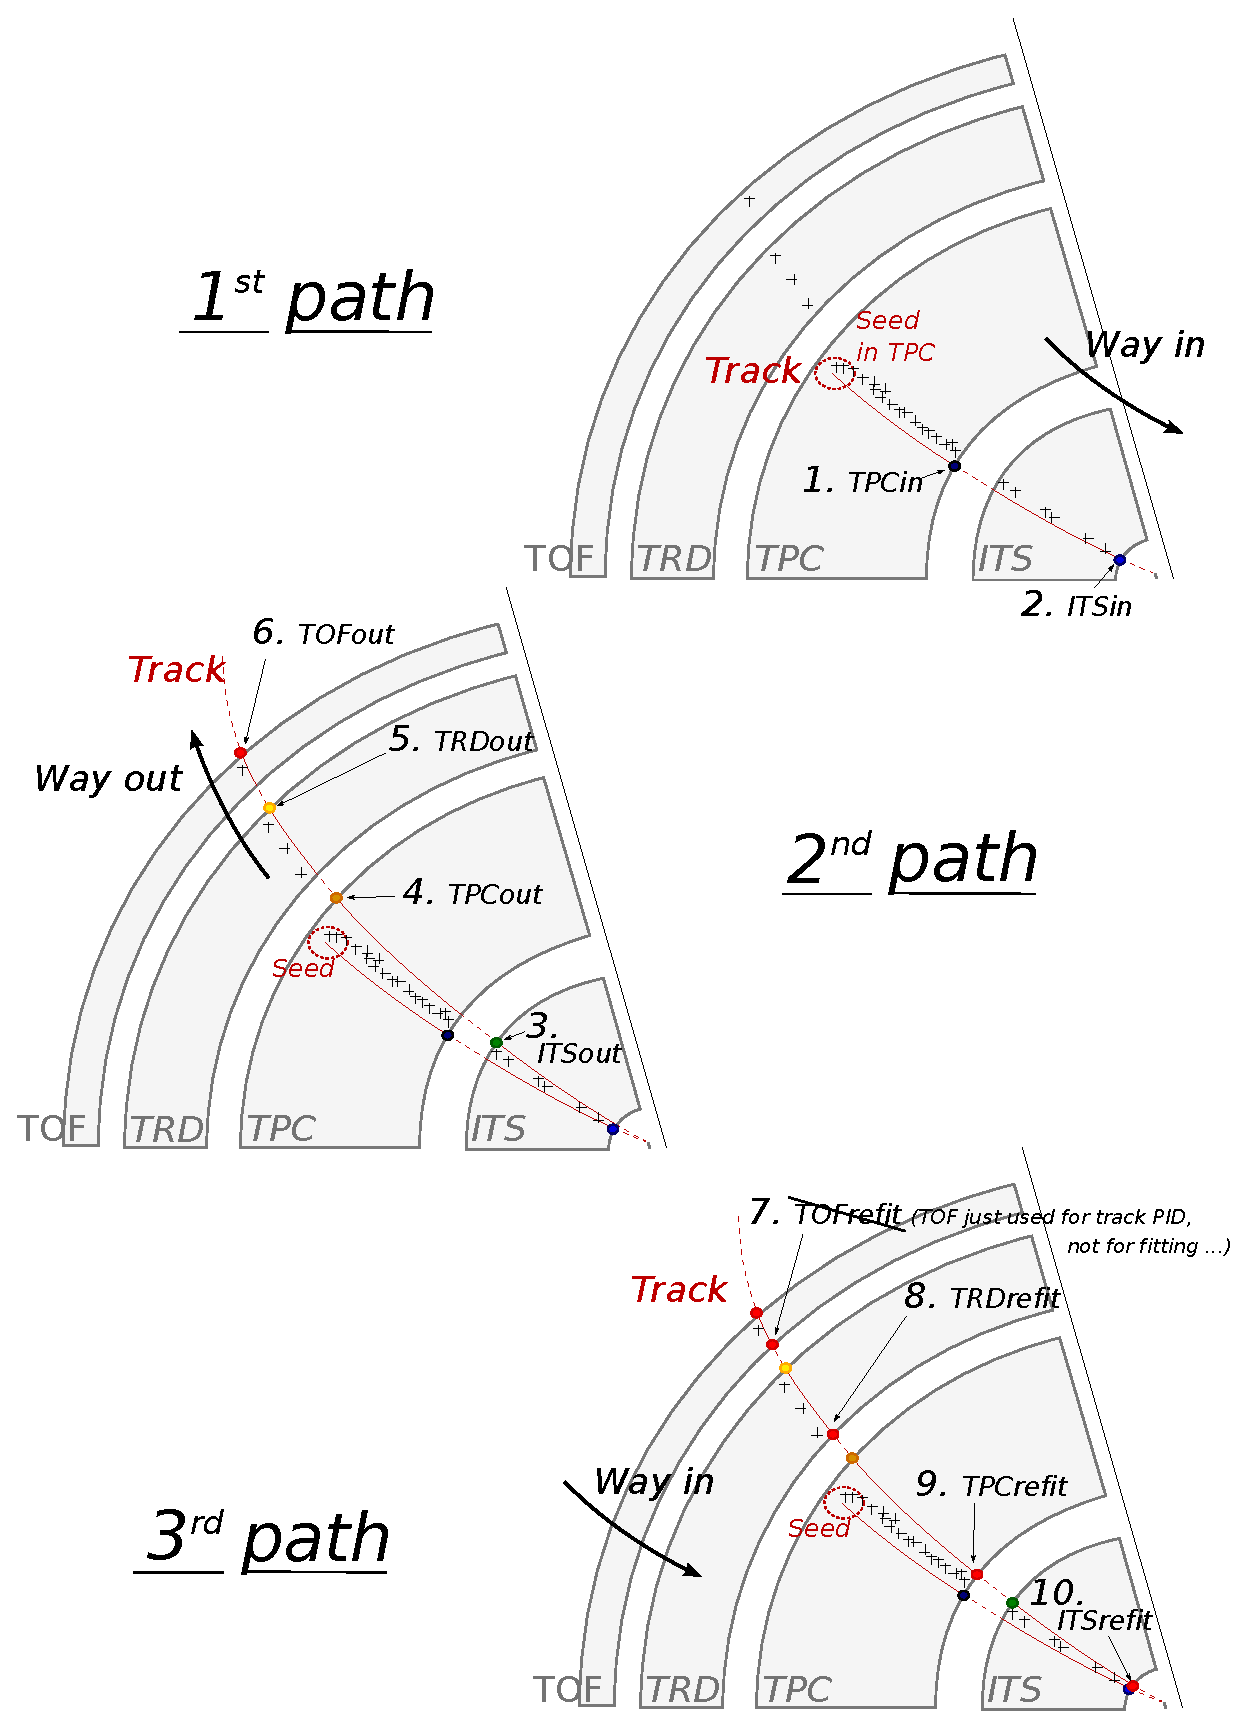
\includegraphics[width=1.05\textwidth]{Figs/Chapter3/Schema-PcpTrackingALICE.eps}
	\caption{Overview\DIFaddbeginFL \DIFaddFL{, at each pass of the Kalman filter, }\DIFaddendFL of the different elements \DIFdelbeginFL \DIFdelFL{of }\DIFdelendFL \DIFaddbeginFL \DIFaddFL{related to }\DIFaddendFL the track reconstruction in ALICE\DIFdelbeginFL \DIFdelFL{, at each pass of the Kalman filter}\DIFdelendFL . Figure taken from \cite{maireTrackReconstructionPrinciple2011}.}
	\label{fig:Kalmanfiltering}
\end{figure}

During this propagation, a preliminary particle identification based on the energy deposit in the TPC gas (see \Sec\ref{subsubsec:TPC}) allows to determine the most probable mass of the track candidate among eight hypothesis: \ePlusMinus, \muPlusMinus, \rmPiPlusMinus, \Kplusmin, \pOrPbar, \rmDeutonPM, \rmTritonPM, \rmHeThreePM or \rmHeFourPM. In cases where there is an ambiguity, the pion mass is assigned by default. From this and the amount of crossed material at each step, energy losses can be corrected on average using the Bethe-Bloch formula (\eq\ref{eq:BetheBloch}). It should be emphasised that all the parameters related to the TPC corresponds, in fact, to those of Ne. This approximation is justified by i) the fact that the TPC gas consists mainly of this element\DIFdelbegin \DIFdel{(until 2017)}\DIFdelend , and ii) the effect is relatively small. 

When all the seeds have reached the inner wall of the TPC, the tracking in the ITS takes over. The reconstructed TPC tracks are extrapolated from the TPC inner wall ($\sim 85$ \cm) to the outermost layers of the ITS (\DIFaddbegin \DIFadd{SSDs at }\DIFaddend 38 and 43 \cm) \DIFdelbegin \DIFdel{, }\DIFdelend that serve as seeds for the track finding in the ITS. Similarly as in the TPC, the seeding procedure produces two kinds of seed: first, one with \DIFaddbegin \DIFadd{a }\DIFaddend vertex constraint, then the other without it. Whatever the hypothesis, they are all propagated as close as possible to the primary vertex, and updated along the way by any cluster passing a proximity cut. Only the highest quality candidates in the ITS from each TPC track are selected. A further check on cluster sharing among each other is performed. In such a case, the tracking algorithm tries to find another candidate and if this fails, the worst of the two tracks receives a special flag for containing a shared cluster \DIFdelbegin \DIFdel{, that is a potentially }\DIFdelend \DIFaddbegin \DIFadd{that is potentially an }\DIFaddend incorrectly assigned cluster.

Once all the ITS-TPC tracks have been formed, the ITS standalone tracking procedure comes into play and uses the remaining clusters to recover unfound tracks in the TPC because of i) their very low momentum or ii) the deadzones between sectors, or iii) decays before reaching the \DIFdelbegin \DIFdel{chamber}\DIFdelend \DIFaddbegin \DIFadd{TPC}\DIFaddend . Formed out of two clusters from the three innermost layers and the preliminary vertex point, the seeds are propagated to the other layers, and updated with clusters passing a proximity cut. Only the track hypothesis with the smallest reduced $\chi^{2}$ is kept, and its assigned clusters are removed from further track finding. The procedure repeats until there are no more track to search. 

Upon completion of the track reconstruction in the ITS, the first stage of the tracking ends with the extrapolation of all tracks to their point of closest approach to the preliminary primary vertex. As in the TPC, energy loss corrections are applied at each propagation step in the ITS, considering the same mass hypothesis as one used previously and assuming that all the materials in the ITS volume (including the beam pipe) are made of Si\footnote{This relies on the same \DIFdelbegin \DIFdel{reasons }\DIFdelend \DIFaddbegin \DIFadd{arguments }\DIFaddend as \DIFdelbegin \DIFdel{the ones mentionned }\DIFdelend \DIFaddbegin \DIFadd{those mentioned }\DIFaddend in the case of the TPC. The \chap\ref{chap:CPTAnalysis} \DIFdelbegin \DIFdel{will showcase }\DIFdelend \DIFaddbegin \DIFadd{addresses }\DIFaddend the limits of this approximation.}.\\

The second stage starts with the \DIFdelbegin \DIFdel{outwards propagation from the primary interaction point to the outermost layers of the ITS, and then towards the TPC outer wall (second path on \fig\ref{fig:Kalmanfiltering}). Based on the track parameters from the first iteration, }\DIFdelend \DIFaddbegin \DIFadd{outward refitting of the track parameters by }\DIFaddend the Kalman filter \DIFdelbegin \DIFdel{goes in the outward direction through }\DIFdelend \DIFaddbegin \DIFadd{using }\DIFaddend the previously associated clusters. \DIFdelbegin \DIFdel{This also allows to calculate }\DIFdelend \DIFaddbegin \DIFadd{It is also during this second pass that }\DIFaddend the track length integral, as well as the expected time of flight for the eight particle mass hypothesis, \DIFdelbegin \DIFdel{which }\DIFdelend \DIFaddbegin \DIFadd{are calculated; both quantities }\DIFaddend are updated at each step. \DIFaddbegin \DIFadd{The propagation procedure goes first from the primary interaction point to the outermost layers of the ITS, and then towards the TPC outer wall (second path on \fig\ref{fig:Kalmanfiltering}). }\DIFaddend When reaching the outer edge of the TPC, the Kalman filter stops updating the track parameters but \DIFdelbegin \DIFdel{continues the propagation }\DIFdelend \DIFaddbegin \DIFadd{the propagation continues in an attempt to match the track with a hit in a }\DIFaddend further detector (TRD, TOF, EMCal, PHOS, HMPID)\DIFdelbegin \DIFdel{for to hit matching}\DIFdelend . The track length integration and time-of-flight \DIFdelbegin \DIFdel{calculations terminates }\DIFdelend \DIFaddbegin \DIFadd{calculation finish }\DIFaddend upon arriving at the TOF detector.\\

At the final stage (third path on \fig\ref{fig:Kalmanfiltering}), starting from the TPC outer wall, all tracks are propagated inwards to their distance of closest approach (DCA) to the preliminary primary vertex. Along the way, their parameters are improved one last time with the previously associated clusters in \DIFdelbegin \DIFdel{each detector}\DIFdelend \DIFaddbegin \DIFadd{the ITS and TPC}\DIFaddend . \\

\begin{figure}[t]
	\centering
	\includegraphics[width=0.9\textwidth]{Figs/Chapter3/PTresolution_vs_1Pt_pPb_2013_PerfPaper-8441.png}
	\caption{Transverse momentum resolution for TPC standalone and ITS-TPC combined tracks, with and without vertex constraint, as a function of $1/\pT$ in p-Pb collisions at \sqrtSnn = 5.02 \tev. The blue squares can not be seen as they overlap \DIFdelbeginFL \DIFdelFL{withe }\DIFdelendFL \DIFaddbeginFL \DIFaddFL{with the }\DIFaddendFL green ones. Figure taken from \cite{alicecollaborationPerformanceALICEExperiment2014}.}
	\label{fig:MomResolution}
\end{figure}

The reconstruction efficiency of TPC standalone tracks saturates around 80-85\% for transverse momentum above 0.5 \gmom, due to the loss of clusters in \DIFdelbegin \DIFdel{the }\DIFdelend deadzones between sectors. At lower \pT, it drops rapidly \DIFdelbegin \DIFdel{because of the dominance }\DIFdelend \DIFaddbegin \DIFadd{due to the preeminence }\DIFaddend of multiple scattering and energy loss in the detector material. Whatever the detector occupancy, the contamination of wrongly associated clusters in the TPC remains low; it does not exceed 3\% for tracks with more than 10\% of fake clusters, even in the most violent heavy-ion collisions.

The TPC track prolongation efficiency to the ITS \DIFdelbegin \DIFdel{shows little dependence on the }\DIFdelend \DIFaddbegin \DIFadd{depends mildly on }\DIFaddend transverse momentum. It reaches $\sim$ 95\% for tracks with at least two associated hits in the ITS, and decreases to about 80\% in pp collisions at \sqrtS = 7 \tev (75\% in Pb-Pb collisions at \sqrtSnn = 2.76 \tev) when they have a minimum of one hit over two SPD layers, the furthest detectors relative to the TPC. The contamination of wrongly associated ITS clusters, though, can be quite high: $\sim$ 30\% of tracks with at least one fake cluster below $\pT < 0.2$ \gmom, $\sim$ 7\% at 1 \gmom, and below 2 \% at 10 \gmom in the most central Pb-Pb collisions.

The \fig\ref{fig:MomResolution} shows the resolution on the inverse transverse momentum for TPC standalone and ITS-TPC combined tracks, extracted from their covariance matrix. This quantity is related to the relative transverse momentum resolution, $\sigma_{\pT}/\pT$, via 
\begin{equation}
\sigma_{1/\pT} = \frac{\sigma_{\pT}}{\pT} \frac{1}{\pT} \quad \Rightarrow \quad \frac{\sigma_{1/\pT}}{1/\pT} = \frac{\sigma_{\pT}}{\pT}.
\end{equation}
\DIFdelbegin \DIFdel{In general, the }\DIFdelend \DIFaddbegin \DIFadd{The }\DIFaddend transverse momentum resolution varies as a function of the transverse momentum; typically, it is at least as good as 0.9\% at $\pT = 1$ \gmom and 6\% at $\pT = 10$ \gmom. Note that the global ITS-TPC tracks always yields to a better relative \pT resolution than those reconstructed only with the TPC. In the latter case, the vertex constraint on the seeding strongly improves the resolution but the effect is negligible with a matching to the ITS detectors.


\subsubsection{Final determination of the primary vertex}
\DIFaddbegin \label{subsubsec:FinalVertexDet}
\DIFaddend 

The end of tracking stage \DIFdelbegin \DIFdel{initiates }\DIFdelend \DIFaddbegin \DIFadd{opens the way towards }\DIFaddend a new determination of the primary vertex, based on the ITS-TPC combined tracks. Unlike the tracklets, their curvature is known, which allows to find the interaction point with a much higher precision.\\

All the global tracks are extrapolated as close as possible to the nominal beam position (or luminous region\footnote{When two beams collide, it gives rise to one or multiple collisions. Their interaction point \textit{a priori} lies anywhere within the region defined by the convolution of the particle distribution -- in other words, the beam size -- of the two incoming beams. Also called \textit{interaction region}, its transverse size is given by $\sigma_{D} = \sigma^{\rm beam} / \sqrt{2}$\DIFaddbegin \DIFadd{, with $\sigma^{\rm beam}$ the bunch size spread. }\DIFaddend \cite{carminatiALICEPhysicsPerformance2004}.}). After rejection of far outliers, the approximate point of closest approach of all selected tracks provides a first estimation of the interaction vertex. From here, in the near vicinity of its true position, a highly precise vertex fit can be performed \cite{karimakiEffectiveVertexFitting1997}. It basically consists in finding the space point that minimises the weighted\footnote{The track weighting has the effect of suppressing the contribution of any remaining outliers.} distance of closest of approach to this same point over all the tracks, as in \eq\ref{eq:SPDVertexer}. 

The precision on the vertex position increases with the number of tracks employed in the fitting algorithm. Therefore, in low-multiplicity events, the fit also includes the nominal beam position as an additional constraint/contribution with an uncertainty corresponding to the transverse size of the luminous region \cite{karimakiEffectiveVertexFitting1997}. Although high-multiplicity events have plenty of tracks available, the high pile-up rate requires a different approach. In order to reduce the contamination from collisions, only tracks coming from the same bunch crossings (identified thanks to the \DIFdelbegin \DIFdel{time information measured in }\DIFdelend \DIFaddbegin \DIFadd{timing information from }\DIFaddend the TOF detectors) can contribute to the same vertex. To further suppress the contribution of outliers, the vertex fitting relies on a more robust technique based on Tukey bisquare weights \cite{alicecollaborationPerformanceALICEExperiment2014}. \\

The \fig\ref{fig:VertexResol} shows the transverse resolution on the primary vertex position as a function of the particle multiplicity per unit pseudo-rapidity in pp at \sqrtS = 7 \tev. As mentioned above, the accuracy on the interaction point position sharply improves with the track multiplicity in the event, reaching $\sim 50$ \mum for $\dNdeta > 15$. With respect to the preliminary vertices found with the SPD tracklets, the final ones determined with global tracks \DIFdelbegin \DIFdel{is }\DIFdelend \DIFaddbegin \DIFadd{are }\DIFaddend better by at least a factor of two. Note that both resolutions scale as the square root of the number of contributing tracks/tracklets \cite{caffarridavideCharmSuppressionPbPb2012}.

\begin{figure}[t]
	\centering
	\includegraphics[width=0.9\textwidth]{Figs/Chapter3/VertexRes-8462.png}
	\caption{Transverse width of the final vertex distribution, in solid markers, in pp collisions at \sqrtS = 7 \tev. Two contributions are separated: the transverse size of the nominal beam position $\sigma_{\rm D}$, and the transverse resolution on the vertex $\alpha / \sqrt{ \left( \dNdeta \right)^{\beta} }$. For comparison, the open markers show the same quantity determined making use of SPD tracklets. Figure taken from \cite{alicecollaborationPerformanceALICEExperiment2014}.}
	\label{fig:VertexResol}
\end{figure}

\subsection{The ALICE offline framework}

\subsubsection{The computing model}

Over the whole LHC Run-2, more than 160 PB of raw data have been collected by the ALICE experiment. Their treatment requires a robust framework, capable of processing them in a reliable and timely fashion. 

To be processed, this volume of data requires an amount of computing resources that can not be concentrated in one place\footnote{There are various reasons. Although the funding agencies invest in the computing equipment of their scientific projects, they focus their investments in their own countries. Even if all computing resources could be put in one place -- let us say, at CERN --, the manpower would be insufficient to ensure the upkeep of such a system.}. Instead, it is spread over different computing centres around the world. In particular, ALICE uses the Worlwide LHC Computing Grid (WLCG), a worldwide computer network infrastructure coordinated by the CERN and shared among all LHC experiments, that includes over 170 computing centres in 42 countries. The WLCG stands as the world's largest computing grid, that provides near real-time access to the LHC data regardless of their physical location \cite{worldwidelhccomputinggridWorldwideLHCComputing}.

\begin{figure}[b]
	\centering
	\includegraphics[width=0.8\textwidth]{Figs/Chapter3/WLCG-Tiers-2021_v3_1.png}
	\caption{The three Tiers of the Worlwide LHC Computing Grid as of 2023, with the list of the thirteen Tier-1 computing centres, with their geographic location. Figure taken from \cite{worldwidelhccomputinggridWorldwideLHCComputing}.}
	\label{fig:WLCG}
\end{figure}

The WLCG computing sites follows a hierarchical structure in layers or \textit{Tiers} as shown in \fig\ref{fig:WLCG}, that provides different levels of data storage and processing. The Tier-0 corresponds to the CERN Data Centre located in Geneva, that directly receives all the raw data from the LHC experiments, keeps one replica (on magnetic tapes) and performs the first reconstruction pass. It also distributes the raw data and the reconstruction output to the thirteen Tier-1 computer centres around the world via high-speed connections between 10 and 100 GB/\second. They share the same roles with CERN, namely safe-keeping the data, finishing their reconstruction and distributing them to the next layer. The Tier-2 regroups about 160 sites, corresponding typically to universities and scientific institutes, that store the data produced by the closest Tier-1 site. Beyond their mass-storage capabilities, they are used to run the physics analysis tasks, produce Monte Carlo simulations, and reprocess the data. A copy of the simulated data is stored in the Tier-1 centres.

Each site relies on four components: networking, hardware, middleware and physics analysis software. The networking -- the backbone of any distributed computing infrastructure -- allows to link together the hundreds of WLCG centres and exchange data with an excellent connectivity thanks to the CERN Internet Exchange Point, the high-bandwidth LHC optical-fibres and the Grid File Transfer Service. Each site can be seen as \DIFaddbegin \DIFadd{a }\DIFaddend computer farm that needs tending to; the hardware component refers to this aspect. It includes maintaining disk and tape servers, providing tools to access the data whatever the storage medium --- via the \textbf{C}ERN \textbf{A}dvanced \textbf{STOR}age system (CASTOR) or CERN EOS --- as well as upgrading regularly the necessary software to operate the Grid system --- from the operating system to the physics analysis software libraries. The middleware corresponds to the software architecture that comes between the operating systems and the physics analysis software; it provides numerous services (interfacing, workload management, monitoring, job submission and execution, etc) in order to access at the titanic CPU power and storage ressources of the Grid. In ALICE, the AliEn system \DIFdelbegin \DIFdel{fill }\DIFdelend \DIFaddbegin \DIFadd{fills }\DIFaddend in this task. Last but not least, the physics analysis software provides the tools to analyse the data.


\subsubsection{The analysis framework, AliRoot}
\label{subsubsec:AliRoot}

As most of the current high-energy experiments -- if not all --, the ALICE offline analysis framework is built upon ROOT, an high-performance object-oriented software developed by the CERN and implemented almost entirely in the C++ programming language. Created in 1994 by René Brun and Fons Rademakers, it provides the mathematical and statistical tools to manipulate large amounts of data and analyse them \cite{renebrunandfonsrademakersROOTObjectOriented}. ROOT sets the \DIFdelbegin \DIFdel{foundation }\DIFdelend \DIFaddbegin \DIFadd{foundations }\DIFaddend for the ALICE offline framework, that divides into two parts during the LHC Run-1 and Run-2:
\begin{itemize}
\item[$\ $] \textbf{AliRoot} \cite{alicecollaborationAliRoot} contains the codes that are common to the whole collaboration. In particular, it includes:
\begin{itemize}
\item[$\bullet$] an interface for running Monte Carlo simulations (from the event generation to the detector response), event visualisation, etc,
\item[$\bullet$] a description of the detector geometry as well as the material budget,
\item[$\bullet$] the alignement and calibration of the detectors, 
\item[$\bullet$] the real and simulated data reconstruction,
\item[$\bullet$] and the management of the data formats;
\end{itemize}
\item[$\ $] \textbf{AliPhysics} \cite{alicecollaborationAliPhysics2023} regroups all the physics analysis tasks to process the collected and simulated events. Each PWG \DIFdelbegin \DIFdel{(\tab\ref{tab:PhysicsBoard} ) }\DIFdelend \DIFaddbegin \DIFadd{in \tab\ref{tab:PhysicsBoard} }\DIFaddend has a dedicated repository.
\end{itemize}

\subsubsection{Data formats}
\label{subsubsec:DataFormats}

Depending on the processing stage, the ALICE data come in three distinct formats with different \DIFdelbegin \DIFdel{level }\DIFdelend \DIFaddbegin \DIFadd{levels }\DIFaddend of abstraction. At the output of the detectors (\Sec\ref{subsec:ALICEDetector}), they take the form of \textit{Raw Data}, that regroups all the cluster informations recorded during a collision. They are collected by the DAQ system before being transmitted at a rate of 200 MB/\second to the Tier-0 site for storage and distribution to Tier-1 data centres. 

In parallel, the raw data undergo their first reconstruction pass at CERN. For pp collisions, it typically takes two minutes per event in pp collisions, mainly in input/output streaming. This first pass yields to an Event Summary Data (ESD) format, that  contains most of the informations related to the reconstruction such as the reconstructed tracks with their associated hits. While \DIFdelbegin \DIFdel{an }\DIFdelend \DIFaddbegin \DIFadd{a pp }\DIFaddend event from raw data occupies about 1 MB of disk space, it reduces to $\sim$ 100 kB in ESD format. 

At the analysis level, the ESD file presents the advantage of having the full knowledge of the tracking and event building, with the possibility of replaying some part of the reconstruction like the V0 and cascade vertexings (see next chapter, \chap\ref{chap:V0CascReconstruction}). However, they are still considered as too heavy and too expensive in terms of CPU time. For that reason, the first pass also produces a file in Analysis Object Data (AOD) format, a lighter version than the ESD counterpart, keeping only the relevant information to extract the physics content from the data. It covers 5 to 10 times less disk space than an ESD file, thereby reducing significatively the processing time by the analysis tasks.\\

Note that the first reconstruction pass only serves to calibrate the TPC, SDD, TOF, T0, luminous region and centrality. The second pass applies the derived calibration, and is then used to improve the calibrations and perform a first data quality assurance. These two reconstruction passes, using only a fraction of the data from each run, provides the input for a more complete and fine-tuned calibration, that is stored in the Offline Conditions DataBase\footnote{In fact, OCDB stores the ideal geometry of the detector,  the alignement objects (\ie corrections on the ideal geometry derived using Millepede algorithm \cite{blobelNewMethodHighPrecision2002}) and the calibration parameters for each data taking period.} (OCDB) and is applied in the third pass. At each stage of the processing, a set of ESD and AOD files is produced. 

\subsubsection{Monte Carlo data}
\label{subsubsec:MCData}

As mentionned in \Sec\ref{subsubsec:AliRoot}, the AliRoot framework has the capability to run Monte Carlo (MC) simulations, that try to reproduce as accurately as possible the stochastic processes observed in the detector by sampling a given set of probability density distributions. Such a simulation consists in two consecutive steps.

It starts with the generation of the event, that simulates a collision as well as the associated physics processes ultimately leading to the creation of primary particles. This first step relies on different models called \textit{event generators}, each having its own paradigm, its own production mechanisms, tuned to mimic the topology the collision (multiplicity, momentum distribution, etc). Among the most commonly used, there are \Pythia \cite{bierlichComprehensiveGuidePhysics2022} and \Herwig \cite{bahrHerwigPhysicsManual2008} for pp collisions, \Epos \cite{pierogEPOSLHCTest2015} for both pp and heavy-ion collisions, \Hijing \cite{wangHIJINGMonteCarlo1994} exclusively for heavy-ion collisions.

After the generation of the event comes the propagation of the primary particles through the ALICE detector. This requires a modelisation of the apparatus in its entirety, from the various elements composing the sub-detectors to their geometric shape and their positioning. It also has to account for noisy or dead channels, detector defects, intensity of the magnetic field, etc. These informations available run by run on OCDB are used to \textit{anchor} the simulation on the \DIFaddbegin \DIFadd{actual }\DIFaddend data taking conditions. The transport and interaction with the detector material typically rely on \DIFaddbegin \DIFadd{dedicated }\DIFaddend softwares, such as \GeantThree \cite{brunGEANTUserGuide1987}, \GeantFour \cite{geant4Geant4HomePage} and \Fluka \cite{battistoniOverviewFLUKACode2015}.

Taking into account the detector response, the energy deposited by the passage of charged particles are converted into digits and then stored in raw data format. From this point, the reconstruction of the event can start. It follows the same procedure as the one applied for real data (\Sec\ref{subsec:EventReco}), yielding to files in ESD and AOD formats.

In order to minimise the disk space usage and the computing time, only a fraction of the total number of events in real data is simulated. The proportion of triggers remains unchanged between real and simulated data, though. For instance, if a run in its entirety has 10\% of high-multiplicity events, its simulated twin will comprise the same fraction of such events.\\

The key point of MC data resides in the presence of the full information about the event. This is often referred as \textit{MC truth}. Each element of the simulation is perfectly known: the number of generated particles, their type, charge, momenta, whether they are primary or secondary, where they deposit energy in the detector giving rise to hits -- the so-called track references --, etc. This copious amount of additional informations opens the \DIFdelbegin \DIFdel{door to other }\DIFdelend \DIFaddbegin \DIFadd{way towards specific }\DIFaddend kinds of investigations. 

When designing a new experiment, it allows to anticipate the results and, if needed, to correct or optimise the current design. It gives also the opportunity to estimate the performances of a detector (typically, the efficiency) and to study its systematic features. Finally, the comparison between the measurements (real data) and the predictions from a given MC model (simulated data) helps to improve our understanding of the underlying physics.\\

It should be mentionned that there exists two classes of MC simulations in high-energy physics. Reproducing as accurately as possible a collision requires tuning the parameters of the simulation such that they correspond to the ones observed in real data, including the decay channels, the branching ratios, etc. This is the standard type of simulations, the \textit{general-purpose} MC production. A limitation arises \DIFdelbegin \DIFdel{from }\DIFdelend \DIFaddbegin \DIFadd{when dealing with }\DIFaddend rare signals: for them to be observed, an unrealistic amount of events would need to be generated. 

Instead, one could resort to an \textit{enriched} MC simulations, in which the abundancy of rare signals is increased. This can be achieved by artificially injecting the particles of interest in the simulation, according to a flat distribution in \pT or rapidity, etc. Another option consists in embedding a pure sample of rare signals into a background event, coming from either a simulation or real data. This is particularly used in p-Pb or Pb-Pb simulations, where \Pythia -- a generator dedicated to pp collisions -- produces an event with an enhanced abundancy in rare signals. However, the topology of the simulated event does not coincide with the one in p-Pb or Pb-Pb collisions. Therefore, the injected event is incorporated into a \Hijing event, that plays the role of a background event\footnote{Note that the background event can \textit{a priori} be re-used several times.}. \newpage  % The ALICE experiment
 \newpage \newpage
%//------ Section 04 -------------------------------------------------------------------------------------------------
\chapter{Identification of V0 particles and cascades}
\label{chap:V0CascReconstruction}
%//-----------------------------------------------------------------------//

The \chap\ref{chap:ParticlePhysics} and \ref{chap:ALICE} have set the scene, it is time for the main actors to come onto stage, \DIFdelbegin \DIFdel{namely }\DIFdelend \DIFaddbegin \DIFadd{that are }\DIFaddend the (multi-)strange baryons \DIFdelbegin \DIFdel{also called }\textit{\DIFdel{hyperons}}%DIFAUXCMD
\footnote{\DIFdel{More precisely, the hyperon family comprises any baryon containing at least one strange quarks, but no heavier quarks such as charm, bottom or top.}}%DIFAUXCMD
\addtocounter{footnote}{-1}%DIFAUXCMD
\DIFdel{. In particular, this chapter lays the foundations for the analysis performed throughout this thesis. }%DIFDELCMD < 

%DIFDELCMD < %%%
\DIFdel{In particular, this chapter of the manuscript establishes the principles of }\DIFdelend \DIFaddbegin \DIFadd{or more precisely, the }\textit{\DIFadd{hyperons}}\DIFadd{. These consist of any baryon containing at least one strange quark, but no heavier quarks such as charm, bottom or top. By describing }\DIFaddend their identification and \DIFaddbegin \DIFadd{the physics interests surrounding their reconstruction, this short chapter }\DIFaddend lays the foundations for the analysis \DIFdelbegin \DIFdel{realised in }\DIFdelend \DIFaddbegin \DIFadd{performed throughout }\DIFaddend this thesis.\DIFaddbegin \\
\DIFaddend 

The first section, \Sec\ref{sec:StrangenessFeatures}, \DIFdelbegin \DIFdel{explains what make strangeness -- andmost }\DIFdelend \DIFaddbegin \DIFadd{underlines the appealing features of strangeness and, }\DIFaddend particularly, (multi-)strange \DIFdelbegin \DIFdel{baryons -- still so appealing, almost 60 years after their first discovery. The \Sec\ref{sec:HyperonId} introduces some key elements related to the }\DIFdelend \DIFaddbegin \DIFadd{particles. The }\DIFaddend hyperons of interest in the present analyses \DIFdelbegin \DIFdel{(\Sec\ref{subsec:V0CascDecays})}\DIFdelend \DIFaddbegin \DIFadd{are specified in the following section, \Sec\ref{sec:HyperonId}}\DIFaddend , as well as the \DIFdelbegin \DIFdel{technique employed to identify them; that is, the topological reconstruction (\Sec\ref{subsec:TopoReco})}\DIFdelend \DIFaddbegin \DIFadd{motivations for this choice. This part also presents the principles for multi-strange baryon identification via topological reconstruction}\DIFaddend . Finally, in connection with \chap\ref{chap:ALICE}, this \DIFdelbegin \DIFdel{small }\DIFdelend \DIFaddbegin \DIFadd{short }\DIFaddend chapter closes on what makes ALICE an \DIFdelbegin \DIFdel{appropriate }\DIFdelend \DIFaddbegin \DIFadd{unique }\DIFaddend experiment for studying strange hadrons\DIFdelbegin \DIFdel{(\Sec\ref{subsec:HyperonAndALICE})}\DIFdelend .


\section{The appealing features of strangeness}
\label{sec:StrangenessFeatures}

\subsection{The strange quark with respect to the other flavours}

\DIFdelbegin \DIFdel{Within nucleons, the strange quark can not be found }\DIFdelend \DIFaddbegin \DIFadd{Similarly as for the charm, bottom and top quarks, there is no strangeness }\DIFaddend among the valence quarks \DIFdelbegin \DIFdel{, including only }\DIFdelend \DIFaddbegin \DIFadd{of the nucleons from the collision beams. These only consist in }\DIFaddend up and down quarks\DIFdelbegin \DIFdel{. It is present in }\DIFdelend \DIFaddbegin \DIFadd{; other flavours can still be found inside }\DIFaddend the sea of quarks \DIFdelbegin \DIFdel{(and anti-quarks) }\DIFdelend and gluons, \DIFdelbegin \DIFdel{although in limited }\DIFdelend \DIFaddbegin \DIFadd{but in a moderate }\DIFaddend amount with respect \DIFaddbegin \DIFadd{to }\DIFaddend those produced during a collision at the LHC \DIFdelbegin \DIFdel{. Therefore, the strange quark }\DIFdelend \DIFaddbegin \DIFadd{energies. From this, there arises an interesting and straightforward aspect of strangeness: all the strange quarks observed }\DIFaddend in the final state \DIFdelbegin \DIFdel{can only originate from }\DIFdelend \DIFaddbegin \DIFadd{hadrons must have been produced in }\DIFaddend the processes that have occured during the collision.

\DIFdelbegin \DIFdel{Quarks can be classified }\DIFdelend \DIFaddbegin \DIFadd{Another property regards the mass of the strange quark. One way of classifying quarks is }\DIFaddend based on whether they preserve (at least, approximatively) or break the chiral symmetry (\Sec\ref{subsubsec:chiralsymmetrybreaking}): the up and down quarks belongs to the first kind and makes part of the \DIFdelbegin \DIFdel{light-flavour }\DIFdelend \DIFaddbegin \DIFadd{light flavour }\DIFaddend sector. Those breaking the chiral symmetry -- the charm, bottom and top quarks -- constitute the \DIFdelbegin \DIFdel{heavy-flavour }\DIFdelend \DIFaddbegin \DIFadd{heavy flavour }\DIFaddend sector. For comparison, the bare mass of the up quark sits at $2.16_{-0.26}^{+0.49}$ \mmass, the down quark at $4.67_{-0.17}^{+0.48}$ \mmass. In contrast, the one of the charm, bottom and top quarks lie around $1.27 \pm 0.02$ \gmass, $4.18_{-0.02}^{+0.03}$ \gmass and $172.69 \pm 0.30$ \gmass respectively \cite{particledatagroupReviewParticlePhysics2022}. From this perspective, the strange quark with its bare mass of \DIFdelbegin \DIFdel{$93.4_{-3.4}^{8.6}$ }\DIFdelend \DIFaddbegin \DIFadd{$93.4_{-3.4}^{+8.6}$ }\DIFaddend \mev holds \DIFdelbegin \DIFdel{a }\DIFdelend \DIFaddbegin \DIFadd{an }\DIFaddend unique position: \DIFdelbegin \DIFdel{while }\DIFdelend its lightweight makes it relatively inexpensive \DIFdelbegin \DIFdel{to create }\DIFdelend \DIFaddbegin \DIFadd{(}\DIFaddend in terms of energy\DIFdelbegin \DIFdel{, it stays }\DIFdelend \DIFaddbegin \DIFadd{) to produce; being }\DIFaddend still much heavier than \DIFaddbegin \DIFadd{the }\DIFaddend up and down quarks \DIFdelbegin \DIFdel{. Therefore, being }\DIFdelend \DIFaddbegin \DIFadd{(by one order of magnitude), this also qualifies it as non-ordinary matter. Thus viewed as }\DIFaddend both light and heavy, the strange \DIFdelbegin \DIFdel{particle represents an exotic quark abundantly produced in the collision}\DIFdelend \DIFaddbegin \DIFadd{quark gives access to an abundant source of non-ordinary matter}\DIFaddend .


\DIFdelbegin %DIFDELCMD < \subsection{The specificities of strange hadrons}
%DIFDELCMD < %%%
\DIFdelend \DIFaddbegin \subsection{The specificity of strange hadrons}
\DIFaddend \label{subsec:SpecStrangeHadrons}

\DIFdelbegin \DIFdel{Once confined within hadrons, the strangeness shows other compelling features. Most of the strange hadrons present a large branching ratio for their decay channel }\DIFdelend \DIFaddbegin \DIFadd{Most of strange hadrons decays }\DIFaddend into charged particles \DIFdelbegin \DIFdel{. Coupled to }\DIFdelend \DIFaddbegin \DIFadd{in their dominant channel. In addition, they also have }\DIFaddend a relatively long lifetime\DIFdelbegin \DIFdel{--- }\DIFdelend \DIFaddbegin \DIFadd{, }\DIFaddend allowing them to fly over \DIFdelbegin \DIFdel{a few centimeters in the detector }\DIFdelend \DIFaddbegin \DIFadd{several centimeters }\DIFaddend before the decay\DIFdelbegin \DIFdel{---, this offers the possibility to reconstruct the different strange particles over a wide range of transverse momentum, making use of their distinctive decay topologies }\DIFdelend \DIFaddbegin \DIFadd{. From these two elements stem the distinctive decay topology of strange particles }\DIFaddend known as V0 or cascade \DIFdelbegin \DIFdel{\mbox{%DIFAUXCMD
\cite{speltzCaracterisationEtatDense2006}}\hspace{0pt}%DIFAUXCMD
. This last point is further developed in the next section, \Sec\ref{subsec:V0CascDecays}. }%DIFDELCMD < 

%DIFDELCMD < %%%
\DIFdel{This allows for a continuous study strange hadrons }\DIFdelend \DIFaddbegin \DIFadd{(\Sec\ref{subsec:V0CascDecays}), that can be used in their reconstruction by associating the different daughter tracks to reform the decay vertex (topological reconstruction, detailed later in \Sec\ref{subsec:TopoReco}) \mbox{%DIFAUXCMD
\cite{speltzCaracterisationEtatDense2006}}\hspace{0pt}%DIFAUXCMD
. This characteristic turns to be particularly interesting as the latter provides a robust identification of strange hadrons over a wide momentum range, }\DIFaddend from low to high \pT.
\DIFdelbegin \DIFdel{Therefore, they stands as }\DIFdelend \DIFaddbegin 

\DIFadd{Consequently, this offers the possibility for a continuous study of strange hadrons over different production regimes, involving soft, intermediary and hard processes such as multi-parton interactions, quark coalescence and jet fragmentation respectively. For that reason, strange particles represents }\DIFaddend prime choice probes to investigate and \DIFaddbegin \DIFadd{thus }\DIFaddend improve our understanding on the evolution of the hadronisation mechanisms\footnote{To be exact, it is not the hadronisation mechanisms that evolves with the transverse momentum but rather their relative weight. For instance, soft processes dominates at low \pT, and hard ones at high \pT. However, \textit{a priori}, there are also soft processes at high momentum -- conversely hard processes at low momentum --, although they represent only a small fraction.} with \DIFdelbegin \DIFdel{the transverse }\DIFdelend momentum.

\section{The multi-strange baryon identification}
\label{sec:HyperonId}

\DIFdelbegin \DIFdel{On the experimental side, the study of strange particles implicitly requires the ability to identify them. In the context of the thesis, the focus is on }\DIFdelend \DIFaddbegin \DIFadd{Among all the strange hadrons, this work focuses on the strangest baryons, containing two or three strange quarks, the so-called }\DIFaddend multi-strange baryons. Excluding the associated resonances, this leaves five particles: three containing two strange quarks -- the \rmXiZero ($uss$), \rmXiM ($dss$) and \rmAxiP ($\bar{d}\bar{s}\bar{s}$) --, and two triple-strange hadrons namely the \rmOmegaM ($sss$) and \rmAomegaP ($\bar{s}\bar{s}\bar{s}$). 

\begin{table}[t]
    \centering
    \begin{tabular}{b{2cm}@{\hspace{0.25cm}} b{2cm}@{\hspace{0.5cm}} b{2cm}@{\hspace{0.25cm}} b{2cm}@{\hspace{0.25cm}} b{3cm}@{\hspace{0.5cm}} b{1.5cm}@{\hspace{0.25cm}}}
    \noalign{\smallskip}\hline\noalign{\smallskip}
	Particle & Strangeness & Mass (\mmass) & Lifetime (\cm) & Decay channel & B.R. \\
    \noalign{\smallskip}\hline \noalign{\smallskip}

    \rmLambda [$u d s$] & $+1$ &1115.683 & 7.89 & \proton [$uud$] \piMinus [$\bar{u} d$] & \textsc{63.9 \%} \\
    \rmAlambda [$\bar{u}\bar{d}\bar{s}$] & $-1$ & 1115.683 & 7.89 & \pbar [$\bar{u} \bar{u} \bar{d}$] \piPlus [$u \bar{d}$] & \textsc{63.9 \%} \\

    \noalign{\smallskip}\hline \noalign{\smallskip}    

    \DIFaddbeginFL \DIFaddFL{\rmXiZero }[\DIFaddFL{$uss$}] & \DIFaddFL{$+2$ }& \DIFaddFL{1314.86 }& \DIFaddFL{8.71 }& \rmLambda [\DIFaddFL{$u d s$}] \DIFaddFL{\piZero }[\DIFaddFL{$u\bar{u}$}] & \textsc{\DIFaddFL{99.6 \%}}\\

    \noalign{\smallskip}\hline \noalign{\smallskip}    

    \DIFaddendFL \rmXiM [$dss$] & $+2$ & 1321.71 & 4.91 & \rmLambda [$u d s$] \piMinus [$\bar{u} d$] & \textsc{99.9 \%}\\
	\rmAxiP [$\bar{d}\bar{s}\bar{s}$] & $-2$ & 1321.71 & 4.91 & \rmAlambda [$\bar{u}\bar{d}\bar{s}$] \piPlus [$u\bar{d}$] & \textsc{99.9 \%}\\

    \noalign{\smallskip}\hline \noalign{\smallskip}

	\rmOmegaM [$sss$] & $+3$ & 1672.45 & 2.461 & \rmLambda [$u d s$] \Kminus [$\bar{d} s$] & \textsc{67.8 \%}\\
	\rmAomegaP [$\bar{s}\bar{s}\bar{s}$] & $-3$ & 1672.45 & 2.461 & \rmAlambda [$\bar{u}\bar{d}\bar{s}$] \Kplus [$u\bar{s}$] & \textsc{67.8 \%}\\

    \noalign{\smallskip}\hline\noalign{\smallskip}
    \end{tabular}
    \caption{Main characteristics of the \rmLambda and the charged multi-strange baryons: quark content, strangeness, tabulated mass and lifetime (\cTau), dominant decay channel with the associated branching ratio (B.R.) \cite{particledatagroupReviewParticlePhysics2022}.}\label{tab:V0CascDecay}
\end{table}

The \tab\ref{tab:V0CascDecay} shows some characteristics of \DIFdelbegin \DIFdel{the four charged ones}\DIFdelend \DIFaddbegin \DIFadd{these five baryons}\DIFaddend , including their dominant decay channel\DIFdelbegin \DIFdel{. These ones are most particularly appealing as they }\DIFdelend \DIFaddbegin \DIFadd{, as well as the mono-strange baryon }\rmLambda \DIFadd{since it appears in all decay channels. Unlike the \rmXiZero, the four charged multi-strange baryons }\DIFaddend share a common feature \DIFdelbegin \DIFdel{that facilitate their identification}\DIFdelend \DIFaddbegin \DIFadd{and a particularly appealing one: in their dominant decay channel}\DIFaddend , they follow a cascade decay topology \DIFdelbegin \DIFdel{in their dominant channel as 
mentionned \ref{subsec:SpecStrangeHadrons}}\DIFdelend \DIFaddbegin \DIFadd{as 
detailed in the next section, \Sec\ref{subsec:V0CascDecays}. For that reason, the present work concentrates on the study of charged multi-strange baryons}\DIFaddend .\\


From now on, the following notation will be used. The \rmXiPM (or \rmOmegaPM) refers to \rmXiM or \rmAxiP (or \rmOmegaM or \rmAomegaP). Conversely, \rmXi (or \rmOmega) means \rmXiM and \rmAxiP (or \rmOmegaM and \rmAomegaP). The same goes for other particles. Moreover, \DIFaddbegin \DIFadd{unless indicated otherwise, }\DIFaddend the term multi-strange baryon \DIFaddbegin \DIFadd{now }\DIFaddend designates only the \rmXiM, \rmAxiP, \rmOmegaM or \rmAomegaP\DIFdelbegin \DIFdel{unless indicated otherwise}\DIFdelend .


\subsection{The V0 and cascade decays}
\label{subsec:V0CascDecays}


The \fig\ref{fig:CascadeDecay} depicts the full cascade decay chain of \rmXi and \rmOmega. After \DIFdelbegin \DIFdel{a flight }\DIFdelend \DIFaddbegin \DIFadd{flying }\DIFaddend over a few centimeters, the multi-strange baryon decays \DIFdelbegin \DIFdel{through weak interaction }\DIFdelend \DIFaddbegin \DIFadd{weakly }\DIFaddend into a charged pion (or kaon for the \rmOmega) and a \rmLambda. The latter being electrically neutral, only the charged meson deposits energy in the different sensitive layers and \DIFaddbegin \DIFadd{thus can }\DIFaddend be detected at this stage; \DIFdelbegin \DIFdel{therefore, }\DIFdelend the meson plays the role of a \textit{bachelor} particle. 
\DIFdelbegin \DIFdel{Although, the }%DIFDELCMD < \rmXiPM %%%
\DIFdel{decays into this channel quasi-systematically, this is only the case for slightly more than 2/3 of the }%DIFDELCMD < \rmOmegaPM%%%
\DIFdel{.
}\DIFdelend 

\begin{figure}[t]
	\centering
	\includegraphics[width=1\textwidth]{Figs/Chapter4/Schema-4TypesDeCascade.eps}
	\caption{Depiction of the full cascade decay chain of the \rmXiM (top left), \rmAxiP (top right), \rmOmegaM (bottom left) and \rmAomegaP (bottom right). Figure taken from \cite{maireFourTypesCascade2011}.}
	\label{fig:CascadeDecay}
\end{figure}

The two decay products continue to travel through the detector, until the baryon daughter decays\DIFdelbegin \DIFdel{via weak interaction }\DIFdelend \DIFaddbegin \footnote{\DIFadd{The bachelor daughter being either a }\rmPiPlusMinus \DIFadd{or }\Kplusmin\DIFadd{, in most cases it does not decay in the detector due to their long lifetime ($\cTau_{\pi} = 7.8045$ }\m \DIFadd{and $\cTau_{\rm K} = 3.711$ }\m\DIFadd{). For those that actually decays in the detector, they are characterised by }\textit{\DIFadd{kink}} \DIFadd{topology due to their decay into a charged particle and a neutral particle.}} \DIFaddend at 63.9\% \DIFaddbegin \DIFadd{via weak interaction }\DIFaddend into two oppositely charged particles: a proton and a pion. Depending on their electric charge, one is called \DIFaddbegin \DIFadd{the }\DIFaddend \textit{positive} \DIFaddbegin \DIFadd{particle }\DIFaddend and the other \DIFaddbegin \DIFadd{the }\DIFaddend \textit{negative} \DIFaddbegin \DIFadd{particle}\DIFaddend . This decay topology is known as V0\footnote{The term \DIFdelbegin \DIFdel{"V0" originates, on one hand, }\DIFdelend \DIFaddbegin \say{V0} \DIFadd{comes }\DIFaddend from the V-shape \DIFaddbegin \DIFadd{decay topology }\DIFaddend formed by the \DIFaddbegin \DIFadd{two oppositely charged }\DIFaddend decay \DIFdelbegin \DIFdel{products, and on the other hand, by the neutral charge of the mother}\DIFdelend \DIFaddbegin \DIFadd{daughters}\DIFaddend .}. Furthermore, the term \DIFdelbegin \DIFdel{"cascade" makes reference }\DIFdelend \DIFaddbegin \say{cascade} \DIFadd{refers }\DIFaddend to the two-steps decay process undergone by the multi-strange \DIFdelbegin \DIFdel{particles. In }\DIFdelend \DIFaddbegin \DIFadd{baryons. Hence, in }\DIFaddend the following, the usage of the term \textit{cascade} may be used to \DIFdelbegin \DIFdel{refer either to }\DIFdelend \DIFaddbegin \DIFadd{mention either the }\DIFaddend \rmXi or \rmOmega, and similarly the term \textit{V0} \DIFdelbegin \DIFdel{to }\DIFdelend \DIFaddbegin \DIFadd{for the }\DIFaddend \rmLambda.

Note that the four cascades on \fig\ref{fig:CascadeDecay} differ only in the nature of the particles involved. On one hand, from the left to right side, the particles are swapped to anti-particles. On the other hand, the larger strangeness content of the \rmOmega imposes the presence of a bachelor particle containing a strange quark (kaon) while, in the \rmXi case, it consists in an light unflavoured meson (pion).
\DIFaddbegin 

\DIFadd{It should also be mentioned that although the }\rmXiPM \DIFadd{decays into this channel quasi-systematically (99.9\%), this is only the case for 67.8\% of the }\rmOmegaPM\DIFadd{.}\DIFaddend \\

\begin{figure}[t]
	\centering
	\includegraphics[width=1\textwidth]{Figs/Chapter4/XiEventDisplay.png}
	\caption{Event display of a simulated Pb-Pb collision in the ALICE detector, with a close up on the ITS. The top part illustrates the typical density of tracks in such environment. The bottom part highlights the cascade decay of a \rmXiM. Figure taken from \cite{alicecollaborationALICEPhysicsPerformance2006}.}
	\label{fig:CascadeDecaySimu}
\end{figure}

The \fig\ref{fig:CascadeDecaySimu} shows the cascade decay of a \rmXiM within the ALICE detector. To make it more apparent, the surrounding tracks have been removed in the bottom left part. The \rmXiPM or \rmOmegaPM being electrically charged, they may loose energy in the detectors and \DIFaddbegin \DIFadd{can }\DIFaddend \textit{a priori} be detected \DIFaddbegin \DIFadd{as any other charged particle}\DIFaddend . Although they can fly over relatively long distance compared to \DIFdelbegin \DIFdel{most of the }\DIFdelend \DIFaddbegin \DIFadd{the vast majority of }\DIFaddend unstable particles, their \cTau \DIFdelbegin \DIFdel{are still }\DIFdelend \DIFaddbegin \DIFadd{remain }\DIFaddend too short to \textit{systematically} reach the innermost detectors at about 3.9 \cm and 7.6 \cm (to be compared to \DIFdelbegin %DIFDELCMD < \cTau%%%
\DIFdel{$_{\Xi}$ }\DIFdelend \DIFaddbegin \DIFadd{$\cTau_{\Xi}$ }\DIFaddend = 4.91 \cm and \DIFdelbegin %DIFDELCMD < \cTau%%%
\DIFdel{$_{\Omega}$ }\DIFdelend \DIFaddbegin \DIFadd{$\cTau_{\Omega}$ }\DIFaddend = 2.461 \cm)\footnote{Note that the detection and tracking of these two multi-strange baryons become possible with the upgraded version of the ITS in the LHC Run-3; the innermost silicon pixel detectors being positioned at a radius of 2.2 \cm and 3.9 \cm in the LHC, the \rmXi and \rmOmega have significantly more chances to leave hits in this detection layers, and therefore to be detected \cite{chinellatoCharmMulticharmBaryon2022}.}. Moreover, the \rmLambda is a neutral particle, hence it can not deposit energy in the sensitive layers. \DIFdelbegin \DIFdel{As a consequence}\DIFdelend \DIFaddbegin \DIFadd{In summary}\DIFaddend , only the \DIFdelbegin \DIFdel{cascade decay products }\DIFdelend \DIFaddbegin \DIFadd{bachelor, the positive and negative particles }\DIFaddend can be detected\DIFdelbegin \DIFdel{, namely the bachelor particle and }\DIFdelend \DIFaddbegin \footnote{\DIFadd{Due to their long lifetime, the detection of the }\rmPiPlusMinus\DIFadd{, }\Kplusmin\DIFadd{, }\proton \DIFadd{and }\pbar \DIFadd{relies on the reconstruction and identification of their associated tracks in the ITS and TPC.}}\DIFadd{. Therefore, it follows that }\DIFaddend the V0 \DIFdelbegin \DIFdel{decay daughters}\DIFdelend \DIFaddbegin \DIFadd{and cascade have to be identified indirectly via their decay topology}\DIFaddend .

The top right part of \fig\ref{fig:CascadeDecaySimu} puts into perspective the difficulty of the reconstructing such a cascade topology. While the \DIFdelbegin \DIFdel{other }\DIFdelend \DIFaddbegin \DIFadd{bottom }\DIFaddend part of the figure shows clearly the \DIFdelbegin %DIFDELCMD < \rmXi %%%
\DIFdel{or }%DIFDELCMD < \rmOmega %%%
\DIFdelend \DIFaddbegin \rmXiM \DIFaddend decay chain, it actually is immersed in a \DIFdelbegin \DIFdel{very crowded environment, from which it can not be isolated easily}\DIFdelend \DIFaddbegin \DIFadd{dense environment}\DIFaddend . In order to identify the multi-strange baryons in the event, the strategy followed in the present work consists in using topological reconstruction.

\subsection{The principles of the topological reconstruction}
\label{subsec:TopoReco}

The \DIFdelbegin \DIFdel{basic idea behind the cascade identification is to use the reconstructed }\DIFdelend \DIFaddbegin \DIFadd{cascade reconstruction is achieved by combining three }\DIFaddend tracks in the event. \DIFdelbegin \DIFdel{Therefore, the }\DIFdelend \DIFaddbegin \DIFadd{The }\DIFaddend association of two tracks allows to build a \rmLambda (or \rmAlambda) candidate, that may in turn be associated to another track (the bachelor) to form a cascade candidate. In a pp collision, the charged particle density\footnote{per unit of pseudo-rapidity} can vary from a few particles up to fifty, and more than a thousands in the most central heavy-ion collisions. The mere association of three tracks \DIFdelbegin \DIFdel{may certainly lead }\DIFdelend \DIFaddbegin \DIFadd{leads inexorably }\DIFaddend to the formation of erroneous candidates, thus constituting a source of \textit{combinatorial} background. In order to suppress the latter, geometric selections -- aimed at singling out the candidates spatially compatible with the expected decay topology -- are introduced; this is the general principle behind topological reconstruction. 

\subsubsection{Formation of the V0 candidates}
\label{subsubsec:V0Formation}

The reconstruction starts with the formation a V0 candidate. The first step consists in identifying \textit{secondary} tracks, that do not originate from the interaction point. They are tagged as such, if the distance of closest approach (DCA) between the considered track and the primary vertex exceeds a critical value\footnote{While one expects for a primary track to have a DCA to the primary vertex equal (or close) to zero, this is the opposite for a secondary track: since it does not originate from the collision point, its DCA to the interaction vertex must necessarily be different from zero.} (\fig\ref{fig:TopologicalRec}, V0.a). 

The second step aims at forming pairs of secondary tracks of opposite charge -- characterised by different curvatures --; by imposing that the DCA between the two tracks is small, only the pairs originating potentially from the same decay point are retained. The secondary vertex is then positioned on the segment defined by the previous DCA, weighted by the \DIFdelbegin \DIFdel{tracks quality }\DIFdelend \DIFaddbegin \DIFadd{quality of the tracks }\DIFaddend (\fig\ref{fig:TopologicalRec}, V0.b).

\afterpage{
\begin{figure}[H]
	\centering
	\includegraphics[width=1\textwidth]{Figs/Chapter3/Schema-ExplicationReconstrCascade-en.eps}
	\caption{Schematic representation of the different topological selections applied in order to first reconstruct V0s (top part), and then cascades (bottom part). Figure taken from \cite{maireTopologicalSelectionsV02011}.}
	\label{fig:TopologicalRec}
\end{figure}
}

The two daughter tracks are then propagated from their initial position (the point of closest approach to the primary vertex, \Sec\ref{subsubsec:TrackReco}) to the secondary decay point\footnote{Most importantly, here the propagation is performed without taking the energy losses into account. This point will be addressed in \chap\ref{chap:CPTAnalysis}}. This allows to calculate all the kinematic quantities of the V0, among which its momentum; the latter being equal to the \DIFdelbegin \DIFdel{sum of the momentum }\DIFdelend \DIFaddbegin \DIFadd{momentum sum }\DIFaddend of the positive and negative particles at the secondary vertex, due to momentum conservation.

\subsubsection{The reconstruction of cascade candidates}
\label{subsubsec:CascadeFormation}

From the sample of V0 candidates (\Sec\ref{subsubsec:V0Formation}), only those compatible with a \rmXiPM or \rmOmegaPM decay are considered. In other words, the reconstruction of a cascade candidate must necessarily go through a secondary V0 that corresponds to either a \rmLambda or \rmAlambda.\\

Primary and secondary V0s are separated resorting to the pointing direction in the lab frame, given by the momentum at the decay vertex. This direction coincides with the straight-line trajectory of the candidate\footnote{If the candidate corresponds to an actual \rmLambda or \rmAlambda (electrically neutral), its trajectory, not being curved under the influence of the magnetic field, must necessarily follow a straight line.} and allows to estimate its DCA to the interaction point (\fig\ref{fig:TopologicalRec}, V0.c). The latter being close to zero for primary V0s, a lower cut on this variable enables their rejection \DIFdelbegin \DIFdel{and }\DIFdelend to retain only those tagged as secondary. 

The identification of the V0 goes through the calculation of \DIFdelbegin \DIFdel{its }\DIFdelend \DIFaddbegin \DIFadd{the }\DIFaddend invariant mass under  the \rmLambda or \rmAlambda hypothesis. This boils down to making an assumption on the mass of each decay daughter. In the case of a \rmLambda, the positive track corresponds to a proton, the negative to a \piMinus (\eq\ref{eq:LambdaInvMass}); conversely, for a \rmAlambda, they are considered as a \piPlus and an anti-proton respectively. If it turns out that \DIFdelbegin \DIFdel{a }\DIFdelend \DIFaddbegin \DIFadd{the }\DIFaddend candidate is, in fact, a true \rmLambda or \rmAlambda, \DIFdelbegin \DIFdel{its }\DIFdelend \DIFaddbegin \DIFadd{the }\DIFaddend reconstructed mass should lie within a window of typically a few \mmass\footnote{The width of the mass window depends directly on the \DIFaddbegin \DIFadd{ALICE performances in terms of }\DIFaddend transverse momentum resolution \DIFdelbegin \DIFdel{of }\DIFdelend \DIFaddbegin \DIFadd{on }\DIFaddend the \DIFdelbegin \DIFdel{decay daughters}\DIFdelend \DIFaddbegin \DIFadd{reconstructed tracks}\DIFaddend .} (\fig\ref{fig:TopologicalRec}, V0.d), centred around the nominal mass of the \rmLambda ($m_{\Lambda} = 1.115683$ \gmass). In most cases, only one of the two mass hypothesis passes the cut\footnote{The misidentification of the daughter particles usually results in \DIFaddbegin \DIFadd{a }\DIFaddend quite different invariant mass.}, making it possible to differentiate between a \rmLambda and a \rmAlambda. 

\begin{align}
M_{\rm candidate}^2(\rmLambda) &= ( E_{\rm pos.} + E_{\rm neg.} )^2 - ( \vec{p}_{\rm pos.} + \vec{p}_{\rm neg.})^2 \\
&= \Big(\sqrt{ \vec{p}_{\rm pos.}^2 + m_{\rm pos.}^2} + \sqrt{ \vec{p}_{\rm neg.}^2 + m_{\rm neg.}^2}\Big)^2 - ( \vec{p}_{\rm pos.} + \vec{p}_{\rm neg.})^2\\
&= \Big(\sqrt{ \vec{p}_{\rm pos.}^2 + m_{p^{+}}^2} + \sqrt{ \vec{p}_{\rm neg.}^2 + m_{\pi^{-}}^2}\Big)^2 - ( \vec{p}_{\rm pos.} + \vec{p}_{\rm neg.})^2 \label{eq:LambdaInvMass}
\end{align}

A last step consists in forming a cascade candidate via the association of a candidate \rmLambda (or \rmAlambda) with any track labelled as secondary\footnote{With the exception of the V0 daughters tracks.} (\fig\ref{fig:TopologicalRec}, Casc.a), playing the role of the bachelor particle. The procedure is analogous to what was done to build a V0 candidate: only pairs with a sufficiently small DCA between the reconstructed \rmLambda (or \rmAlambda) and the bachelor are considered (\fig\ref{fig:TopologicalRec}, Casc.b); primary \DIFdelbegin \DIFdel{and }\DIFdelend cascades are set apart from secondary ones by introducing the \textit{pointing angle}. The latter corresponds to the angle defined by the direction of propagation (or pointing direction) of the candidate, and the line joining the primary and secondary vertices. This angle should be small for a primary candidate and, even though the magnetic field is bending their trajectory, the change in direction remains \DIFdelbegin \DIFdel{low}\DIFdelend \DIFaddbegin \DIFadd{moderate}\DIFaddend . This selection usually goes through the cosine of the pointing angle, that is constrained to be close to unity in order to validate the cascade as primary (\fig\ref{fig:TopologicalRec}, Casc.c).

The V0 candidate is subject to the same cut. Due to its large mass compared to the one of the bachelor, the reconstructed \rmLambda (or \rmAlambda) takes up most of the cascade momentum, and so most of the pointing direction. As a consequence, in order to ensure that the V0 actually originates from a \rmXiPM or \rmOmegaPM decay, the cosine of its pointing angle has to be close to unity.\\

As a final topological selection, the cascade and V0 decay vertices must lie within a certain confidence area, in the transverse plane (\fig\ref{fig:TopologicalRec}, Casc.d). Close to the interaction point, at small radii, the combinatorial background \DIFdelbegin \DIFdel{dominates }\DIFdelend \DIFaddbegin \DIFadd{is overwhelming }\DIFaddend due to the high density of tracks. Conversely, at large distance, the probability of finding a \rmXiPM or \rmOmegaPM becomes extremely low. For comparison, the inner wall of the TPC ($\sim$ 85 \cm) \DIFdelbegin \DIFdel{situates }\DIFdelend \DIFaddbegin \DIFadd{lie }\DIFaddend at $\sim 18$ $\cTau_{\Xi}$ and $\sim 35$ $\cTau_{\Omega}$. At such distance, the \rmXiPM and \rmOmegaPM survival probabilities are about 2\% and 0.001\%\footnote{Considering a \DIFaddbegin \DIFadd{high-momentum }\DIFaddend cascade \DIFdelbegin \DIFdel{with a momentum }\DIFdelend of 5 \gmom.} respectively. Therefore, the decay vertices of both cascade and V0 must be located beyond a radius deemed critical; those decaying too far away with respect to their lifetime are rejected\DIFaddbegin \footnote{\DIFadd{Notice that one consists in a selection on the radial position of the decay vertices, the other a cut on their 3D location.}}\DIFaddend .

\subsubsection{Invariant mass of the cascade candidates}

At this stage, the topological reconstruction is over; each triplet of tracks forms a cascade candidate, that can correspond to a \rmXiPM, a \rmOmegaPM or some residual background. \DIFdelbegin \DIFdel{This }\DIFdelend \DIFaddbegin \DIFadd{The }\DIFaddend distinction is made based on the invariant mass of each candidate (\eq\ref{eq:CascInvMass}).


\begin{align}
M_{\rm candidate}^2( \textrm{casc.}) &= ( E_{\rm V0} + E_{\rm bach.} )^2 - ( \vec{p}_{\rm V0} + \vec{p}_{\rm bach.})^2 \\
&= \Big(\sqrt{ \vec{p}_{\rm V0}^2 + m_{\rmLambda}^2} + \sqrt{ \vec{p}_{\rm bach.}^2 + m_{\rm bach.}^2}\Big)^2 - ( \vec{p}_{\rm V0} + \vec{p}_{\rm bach.})^2 \label{eq:CascInvMass}
\end{align}

\begin{align}
M_{\rm candidate}^2( \rmXiPM ) &= \Big(\sqrt{ \vec{p}_{\rm V0}^2 + m_{\rmLambdaPM}^2} + \sqrt{ \vec{p}_{\rm bach.}^2 + m_{\pi^{\pm}}^2}\Big)^2 - ( \vec{p}_{\rm V0} + \vec{p}_{\rm bach.})^2 \label{eq:XiInvMass} \\
M_{\rm candidate}^2( \rmOmegaPM ) &= \Big(\sqrt{ \vec{p}_{\rm V0}^2 + m_{\rmLambdaPM}^2} + \sqrt{ \vec{p}_{\rm bach.}^2 + m_{\rm K^{\pm}}^2}\Big)^2 - ( \vec{p}_{\rm V0} + \vec{p}_{\rm bach.})^2 
\label{eq:OmegaInvMass}
\end{align}

For each association of three particles, two invariant masses are calculated: one under the hypothesis of a \rmXiPM candidate (\eq\ref{eq:XiInvMass}), the other for a \rmOmegaPM candidate (\eq\ref{eq:OmegaInvMass}). Notice that, contrarily to the \rmLambda and \rmAlambda cases, the invariant mass is the same for the particle (\rmXiM, \rmOmegaM) and the anti-particle (\rmAxiP, \rmAomegaP). In addition, the masses of the daughter particles involved in \eq\ref{eq:XiInvMass} and \ref{eq:OmegaInvMass} correspond, in fact, to the nominal values from the PDG \cite{particledatagroupReviewParticlePhysics2022}; most importantly, the reconstructed mass of the V0 is not being used here. As long as the latter has been identified as a \rmLambdaPM (\ie its mass fits into a certain tolerance window, \Sec\ref{subsubsec:CascadeFormation}), this choice has the advantage of limiting the deterioration on the cascade invariant mass resolution. \\

Although the invariant mass allows to distinguish a \rmXiPM from a \rmOmegaPM, there exists a region where this is not possible anymore. The \fig\ref{fig:MassXiVsOmega} shows the invariant mass distribution of cascade candidates assuming a \rmOmegaM \DIFdelbegin \DIFdel{and }\DIFdelend \DIFaddbegin \DIFadd{as a function of the same candidate under the hypothesis of a }\DIFaddend \rmXiM. There are two discernible and perpendicular mass bands, each one corresponding to true population of one of two considered species. At their intersection, the two species become indistinguishables, which results in an increased background in this region: a candidate identified as \rmXiM may, in fact, reveal to be a \rmOmegaM, and vice-versa. 

This additional background impacts each kind of cascade in different proportions, though. Since the population of true \rmXiM is much larger than the one of \rmOmegaM\footnote{That is because the \rmXi are typically ten times more produced than the \rmOmega \cite{alicecollaborationProductionLightflavorHadrons2020}.}, the latter constitutes a marginal source of background with respect to the \rmXiM. Conversely, the true \rmXiM -- particularly in the low mass region -- represent a considerable source of background for the \rmOmegaM. As a consequence, in the context of the reconstruction of \rmOmegaPM baryons, any candidates also identified as a \rmXiPM --- that is, with an invariant mass under the assumption of a \rmXiPM within a window of few \mmass around \mPDG\rmXi --- are rejected. 

\begin{figure}[!t]
	\includegraphics[width=0.9\textwidth]{Figs/Chapter4/MassXiVsOmegaMinus.eps}
	\caption{Invariant mass distribution under the \rmOmegaM and \rmXiM mass hypotheses, each cascade candidate can be seen under one hypothesis or the other (\eq\ref{eq:XiInvMass} and \ref{eq:OmegaInvMass}). The dashed lines show the mass rejection $\mPDG\rmXi \pm 0.008 \gmass$, applied in the reconstruction of a \rmOmegaPM candidate.}
	\label{fig:MassXiVsOmega}
\end{figure}



\subsection{The context of hyperon reconstruction in ALICE}
\label{subsec:HyperonAndALICE}

In view of the characteristics of multi-strange baryons, it appears plainly that their reconstruction require excellent detection capabilities. In that regard, few experiments can compete with the performances of the ALICE detector \DIFdelbegin \DIFdel{, }\DIFdelend at mid-rapidity.

As already outlined in \Sec\ref{subsec:ALICEDetector}, the high granularity of its inner tracker allows to reconstruct the primary vertex, as well as the secondary vertices from V0 and cascade decays, with a precision better than 100 \mum\footnote{Not to mention the resolution on the DCA of the daughter tracks to the primary vertex of about 30 \mum \cite{alicecollaborationPerformanceALICEExperiment2014}.}. Thanks to its large lever arm and almost continuous sampling of the particle trajectory, the TPC 
provides an excellent momentum measurement with a resolution of 0.7\%\footnote{This obviously depends on the track momentum; here this is for \pT = 1 \gmom.} \cite{alicecollaborationALICEPhysicsPerformance2006}, as well as a robust particle identification\DIFdelbegin \DIFdel{, on }\DIFdelend \DIFaddbegin \DIFadd{. Hence, the TPC ensures an efficient reconstruction and identification of }\DIFaddend the hyperon's decay daughters\DIFaddbegin \DIFadd{, and thus of the hyperon itself}\DIFaddend . Coupled with its extremely low material budget (13\% \Xzero) and \DIFdelbegin \DIFdel{a }\DIFdelend moderate magnetic field of 0.5 T, the strange hadron reconstruction can be performed over a wide momentum range and particularly, at low \pT, where the most important part of the production is.

Furthermore, the experiment benefits from the high-energy collisions delivered by the LHC. At such energies, \DIFdelbegin \DIFdel{hyperons and anti-hyperons }\DIFdelend \DIFaddbegin \DIFadd{matter and anti-matter }\DIFaddend are produced in almost equal proportions\DIFdelbegin \DIFdel{. All these elements makes ALICE }\DIFdelend \DIFaddbegin \DIFadd{, offering the opportunity to study simultaneously hyperons and anti-hyperons. For all these reasons, ALICE stands as }\DIFaddend a perfectly suited experiment to \DIFdelbegin \DIFdel{study }\DIFdelend \DIFaddbegin \DIFadd{analyse }\DIFaddend multi-strange baryons. \\

It should be emphasised that the cascade reconstruction varies with the track density, that goes from a few charged particles in pp collisions up to 2000 in the most central Pb-Pb collisions at \sqrtSnn = 5.02 \tev \DIFdelbegin \DIFdel{\mbox{%DIFAUXCMD
\cite{alicecollaborationCentralityDependenceChargedparticle2016}}\hspace{0pt}%DIFAUXCMD
}\DIFdelend \DIFaddbegin \DIFadd{\mbox{%DIFAUXCMD
\cite{alicecollaborationCentralityDependenceChargedParticle2016}}\hspace{0pt}%DIFAUXCMD
}\DIFaddend . In heavy-ion collisions, the enormous amount of tracks means a larger background, but also a larger number of contributor for the primary vertex determination and hence a better resolution on its position. This is in contrast with the pp environment, where the events are less dense but with a poorer quality on the interaction point location. Therefore, the topological selections \DIFdelbegin \DIFdel{should }\DIFdelend \DIFaddbegin \DIFadd{shall }\DIFaddend be adapted for each environment, as these differences may lead to various biases on the DCA to the primary vertex, pointing angles, etc. 

Also, a compromise has to be made between purity and reconstruction efficiency. In both cases, the key point revolves around the treatement of the background, which depends on the physics analysis. For example, if the background -- or more precisely, its shape -- is known in advance, the latter becomes tolerable as it can be subtracted \DIFaddbegin \DIFadd{later}\DIFaddend ; thus, one may favour a high efficiency (\ie relatively loose selections). In the reverse situation  where the background is \DIFdelbegin \DIFdel{not known}\DIFdelend \DIFaddbegin \DIFadd{unknown}\DIFaddend , it seems preferable to apply tighter cuts in order to keep a signal with a low level of contamination\DIFdelbegin \DIFdel{and thus ensure }\DIFdelend \DIFaddbegin \DIFadd{, thus ensuring }\DIFaddend a high signal purity.

 \newpage  % V0 and cascade reconstruction
 \newpage %//------ Section 03 -------------------------------------------------------------------------------------------------
\chapter{Mass measurements of multi-strange baryons in pp collisions at \sqrtS = 13 TeV}
\label{chap:CPTAnalysis}
%//-----------------------------------------------------------------------// \newpage  % The CPT analysis
 \newpage %//------ Section 04 -------------------------------------------------------------------------------------------------
\chapter{Analysis of the correlated production of strange hadrons}
\label{chap:CorrelatedAnalysis}
%//-----------------------------------------------------------------------// \newpage  % Correlation analysis
%%//------ Section 05 -------------------------------------------------------------------------------------------------
\chapter{Discussion and future prospects}
\label{sec:Section05} % Discusssion
 \newpage %//------ Section 07 -------------------------------------------------------------------------------------------------
\chapter{Discussion and conclusion}
\label{chap:Conclusion}
%//-----------------------------------------------------------------------//



\newpage


 \newpage  % Conclusion



% http://en.wikibooks.org/wiki/LaTeX/Bibliography_Management#Bibliography_in_the_table_of_contents
\cleardoublepage % pour fermer le dernier paragraphe du chapitre précédent (ccl°)
\phantomsection % With hyperref package, you should also use \phantomsection command to enable hyperlinking from the table of contents to bibliography.




%______________________________________________________________________________
%______________________________________________________________ Bibliography
% (In case of using bibtex generate the bbl requested by arXiv)




\footnotesize

%\bibliographystyle{utphys}   
\bibliographystyle{myJHEP} % http://jhep.sissa.it/jhep/help/JHEP_TeXclass.jsp


% http://en.wikibooks.org/wiki/LaTeX/Bibliography_Management#Bibliography_in_the_table_of_contents
\cleardoublepage % pour fermer le dernier paragraphe du chapitre précédent (ccl°)
\phantomsection % With hyperref package, you should also use \phantomsection command to enable hyperlinking from the table of contents to bibliography.

\addcontentsline{toc}{section}{References} 
\providecommand{\href}[2]{#2}\begingroup\raggedright\DIFdelbegin %DIFDELCMD < \begin{thebibliography}{10}
%DIFDELCMD < %%%
\DIFdelend \DIFaddbegin \begin{thebibliography}{100}
\DIFaddend 

\bibitem{carruthersQuarkiumBizarreFermi1974}
P.~A. Carruthers, {\em Quarkium: {{A}} Bizarre {{Fermi}} Liquid}.
\newblock 1974.

\bibitem{harringtonHighDensityPhaseTransitions1974}
B.~J. Harrington and A.~Yildiz, {\it High-{{Density Phase Transitions}} in
  {{Gauge Theories}}},  {\textsl{Phys. Rev. Lett.}} {\footnotesize \bf 33}
  (July, 1974) 324--327.
  \href{http://dx.doi.org/10.1103/PhysRevLett.33.324}{\footnotesize
  \textrm{\textsc{doi l}ink}}.

\bibitem{collinsSuperdenseMatterNeutrons1975}
J.~C. Collins and M.~J. Perry, {\it Superdense {{Matter}}: {{Neutrons}} or
  {{Asymptotically Free Quarks}}?},  {\textsl{Phys. Rev. Lett.}} {\footnotesize
  \bf 34} (May, 1975) 1353--1356.
  \href{http://dx.doi.org/10.1103/PhysRevLett.34.1353}{\footnotesize
  \textrm{\textsc{doi l}ink}}.

\bibitem{NewStateMatter2023}
{\it New {{State}} of {{Matter}} created at {{CERN}}},
  https://home.web.cern.ch/news/press-release/cern/new-state-matter-created-cern,
  Jan. 2023.

\bibitem{ludlamHUNTINGQUARKGLUON2005}
T.~Ludlam and S.~Aronson, {\it {{HUNTING THE QUARK GLUON PLASMA}}.},
  https://digital.library.unt.edu/ark:/67531/metadc1411284/, Apr. 2005.

\bibitem{arseneQuarkGluonPlasma2005}
I.~Arsene, {\it Quark {{Gluon Plasma}} an {{Color Glass Condensate}} at
  {{RHIC}}? {{The}} perspective from the {{BRAHMS}} experiment},
  {\textsl{Nuclear Physics A}} {\footnotesize \bf 757} (Aug., 2005) 1--27,
  [\href{https://arxiv.org/abs/nucl-ex/0410020}{{\footnotesize
  nucl-ex/0410020}}].
  \href{http://dx.doi.org/10.1016/j.nuclphysa.2005.02.130}{\footnotesize
  \textrm{\textsc{doi l}ink}}.

\bibitem{alPHOBOSPerspectiveDiscoveries2005}
B.~B.~B. et~{al}, {\it The {{PHOBOS Perspective}} on {{Discoveries}} at
  {{RHIC}}},  {\textsl{Nuclear Physics A}} {\footnotesize \bf 757} (Aug., 2005)
  28--101, [\href{https://arxiv.org/abs/nucl-ex/0410022}{{\footnotesize
  nucl-ex/0410022}}].
  \href{http://dx.doi.org/10.1016/j.nuclphysa.2005.03.084}{\footnotesize
  \textrm{\textsc{doi l}ink}}.

\bibitem{phenixcollaborationFormationDensePartonic2005}
P.~Collaboration and K.~Adcox, {\it Formation of dense partonic matter in
  relativistic nucleus-nucleus collisions at {{RHIC}}: {{Experimental}}
  evaluation by the {{PHENIX}} collaboration},  {\textsl{Nuclear Physics A}}
  {\footnotesize \bf 757} (Aug., 2005) 184--283,
  [\href{https://arxiv.org/abs/nucl-ex/0410003}{{\footnotesize
  nucl-ex/0410003}}].
  \href{http://dx.doi.org/10.1016/j.nuclphysa.2005.03.086}{\footnotesize
  \textrm{\textsc{doi l}ink}}.

\bibitem{starcollaborationExperimentalTheoreticalChallenges2005}
S.~Collaboration and J.~Adams, {\it Experimental and {{Theoretical Challenges}}
  in the {{Search}} for the {{Quark Gluon Plasma}}: {{The STAR
  Collaboration}}'s {{Critical Assessment}} of the {{Evidence}} from {{RHIC
  Collisions}}},  {\textsl{Nuclear Physics A}} {\footnotesize \bf 757} (Aug.,
  2005) 102--183, [\href{https://arxiv.org/abs/nucl-ex/0501009}{{\footnotesize
  nucl-ex/0501009}}].
  \href{http://dx.doi.org/10.1016/j.nuclphysa.2005.03.085}{\footnotesize
  \textrm{\textsc{doi l}ink}}.

\bibitem{ThirdRunLarge2023}
{\it The third run of the {{Large Hadron Collider}} has successfully started},
  https://home.cern/news/news/cern/third-run-large-hadron-collider-has-successfully-started,
  Jan. 2023.

\bibitem{alicecollaborationUpgradeALICEExperiment2014}
T.~A. ALICE~Collaboration, {\it Upgrade of the {{ALICE Experiment}}: {{Letter
  Of Intent}}},  {\textsl{J. Phys. G: Nucl. Part. Phys.}} {\footnotesize \bf
  41} (July, 2014) 087001.
  \href{http://dx.doi.org/10.1088/0954-3899/41/8/087001}{\footnotesize
  \textrm{\textsc{doi l}ink}}.

\bibitem{alicecollaborationCharacterizingInitialConditions2022}
A.~Collaboration, {\it Characterizing the initial conditions of heavy-ion
  collisions at the {{LHC}} with mean transverse momentum and anisotropic flow
  correlations},  {\textsl{Physics Letters B}} {\footnotesize \bf 834} (Nov.,
  2022) 137393, [\href{https://arxiv.org/abs/2111.06106}{{\footnotesize
  arXiv:2111.06106}}].
  \href{http://dx.doi.org/10.1016/j.physletb.2022.137393}{\footnotesize
  \textrm{\textsc{doi l}ink}}.

\bibitem{schotterMultidifferentialInvestigationStrangeness2023}
R.~Schotter, {\it A multi-differential investigation of strangeness production
  in pp collisions with {{ALICE}}},  Feb. 2023.
\newblock \href{https://arxiv.org/abs/2302.00454}{{\footnotesize
  arXiv:2302.00454}}.

\bibitem{schotterQCDLHC2022}
{Schotter}, {\it {{QCD}}@{{LHC2022}}},
  https://indico.cern.ch/event/1150707/contributions/5112603/.

\bibitem{pullmanAtomHistoryHuman1998}
B.~Pullman, {\em The Atom in the History of Human Thought}.
\newblock {New York : Oxford University Press}, 1998.

\bibitem{thomsonXLCathodeRays1897}
J.~J. Thomson, {\it {{XL}}. {{Cathode Rays}}},  {\textsl{The London, Edinburgh,
  and Dublin Philosophical Magazine and Journal of Science}} {\footnotesize \bf
  44} (Oct., 1897) 293--316.
  \href{http://dx.doi.org/10.1080/14786449708621070}{\footnotesize
  \textrm{\textsc{doi l}ink}}.

\bibitem{lattesProcessesInvolvingCharged1947}
C.~M.~G. Lattes, H.~Muirhead, G.~P.~S. Occhialini, and C.~F. Powell, {\it
  Processes {{Involving Charged Mesons}}},  {\textsl{Nature}} {\footnotesize
  \bf 159} (May, 1947) 694--697.
  \href{http://dx.doi.org/10.1038/159694a0}{\footnotesize \textrm{\textsc{doi
  l}ink}}.

\bibitem{rochesterdr.EvidenceExistenceNew1947}
G.~D. ROCHESTERDr. and C.~C. BUTLERDr., {\it Evidence for the {{Existence}} of
  {{New Unstable Elementary Particles}}},  {\textsl{Nature}} {\footnotesize \bf
  160} (Dec., 1947) 855--857.
  \href{http://dx.doi.org/10.1038/160855a0}{\footnotesize \textrm{\textsc{doi
  l}ink}}.

\bibitem{hopperEvidenceConcerningExistence1950}
V.~D. Hopper and S.~Biswas, {\it Evidence {{Concerning}} the {{Existence}} of
  the {{New Unstable Elementary Neutral Particle}}},  {\textsl{Phys. Rev.}}
  {\footnotesize \bf 80} (Dec., 1950) 1099--1100.
  \href{http://dx.doi.org/10.1103/PhysRev.80.1099}{\footnotesize
  \textrm{\textsc{doi l}ink}}.

\bibitem{chamberlainObservationAntiprotons1955}
O.~Chamberlain, E.~Segr{\`e}, C.~Wiegand, and T.~Ypsilantis, {\it Observation
  of {{Antiprotons}}},  {\textsl{Phys. Rev.}} {\footnotesize \bf 100} (Nov.,
  1955) 947--950.
  \href{http://dx.doi.org/10.1103/PhysRev.100.947}{\footnotesize
  \textrm{\textsc{doi l}ink}}.

\bibitem{reinesNeutrino1956}
F.~Reines and C.~L. COWANjun., {\it The {{Neutrino}}},  {\textsl{Nature}}
  {\footnotesize \bf 178} (Sept., 1956) 446--449.
  \href{http://dx.doi.org/10.1038/178446a0}{\footnotesize \textrm{\textsc{doi
  l}ink}}.

\bibitem{danbyObservationHighEnergyNeutrino1962}
G.~Danby, J.-M. Gaillard, K.~Goulianos, et~al., {\it Observation of
  {{High-Energy Neutrino Reactions}} and the {{Existence}} of {{Two Kinds}} of
  {{Neutrinos}}},  {\textsl{Phys. Rev. Lett.}} {\footnotesize \bf 9} (July,
  1962) 36--44. \href{http://dx.doi.org/10.1103/PhysRevLett.9.36}{\footnotesize
  \textrm{\textsc{doi l}ink}}.

\DIFaddbegin \bibitem{barnesObservationHyperonStrangeness1964a}
\DIFadd{V.~E. Barnes, P.~L. Connolly, D.~J. Crennell, et~al., }{\it \DIFadd{Observation of a
  }{{\DIFadd{Hyperon}}} \DIFadd{with }{{\DIFadd{Strangeness Minus Three}}}}\DIFadd{,  }{\textsl{\DIFadd{Phys. Rev. Lett.}}}
  {\footnotesize \bf \DIFadd{12}} \DIFadd{(Feb., 1964) 204--206.
  }\href{http://dx.doi.org/10.1103/PhysRevLett.13.585}{\footnotesize
  \textrm{\textsc{\DIFadd{doi l}}\DIFadd{ink}}}\DIFadd{.
}

\DIFaddend \bibitem{serwayModernPhysics2004}
R.~Serway, C.~Moses, and C.~Moyer, {\em Modern {{Physics}}}.
\newblock {Cengage Learning}, 2004.

\bibitem{kochAspectsChiralSymmetry1997}
V.~Koch, {\it Aspects of {{Chiral Symmetry}}},  {\textsl{Int. J. Mod. Phys. E}}
  {\footnotesize \bf 06} (June, 1997) 203--249,
  [\href{https://arxiv.org/abs/nucl-th/9706075}{{\footnotesize
  nucl-th/9706075}}].
  \href{http://dx.doi.org/10.1142/S0218301397000147}{\footnotesize
  \textrm{\textsc{doi l}ink}}.

\bibitem{peskinIntroductionQuantumField2018}
M.~E. Peskin, {\em An {{Introduction To Quantum Field Theory}}}.
\newblock {CRC Press}, {Boca Raton}, Jan. 2018.

\bibitem{braibantParticlesFundamentalInteractions2012}
S.~Braibant, G.~Giacomelli, and M.~Spurio, {\em Particles and {{Fundamental
  Interactions}}}.
\newblock Undergraduate {{Lecture Notes}} in {{Physics}}. {Springer
  Netherlands}, {Dordrecht}, 2012.

\bibitem{noetherInvariantVariationProblems1971}
E.~Noether and M.~A. Tavel, {\it Invariant {{Variation Problems}}},
  {\textsl{Transport Theory and Statistical Physics}} {\footnotesize \bf 1}
  (Jan., 1971) 186--207,
  [\href{https://arxiv.org/abs/physics/0503066}{{\footnotesize
  physics/0503066}}].
  \href{http://dx.doi.org/10.1080/00411457108231446}{\footnotesize
  \textrm{\textsc{doi l}ink}}.

\bibitem{DefinitionGAUGE2023}
{\it Definition of {{GAUGE}}},
  https://www.merriam-webster.com/dictionary/gauge, Feb. 2023.

\bibitem{sozziTestsDiscreteSymmetries2019}
M.~S. Sozzi, {\it Tests of discrete symmetries},  {\textsl{J. Phys. G: Nucl.
  Part. Phys.}} {\footnotesize \bf 47} (Nov., 2019) 013001.
  \href{http://dx.doi.org/10.1088/1361-6471/ab4822}{\footnotesize
  \textrm{\textsc{doi l}ink}}.

\bibitem{lehnertCPTSymmetryIts2016}
R.~Lehnert, {\it {{CPT Symmetry}} and {{Its Violation}}},  {\textsl{Symmetry}}
  {\footnotesize \bf 8} (Nov., 2016) 114.
  \href{http://dx.doi.org/10.3390/sym8110114}{\footnotesize \textrm{\textsc{doi
  l}ink}}.

\bibitem{sachsPhysicsTimeReversal1987}
R.~G. Sachs, {\em The {{Physics}} of {{Time Reversal}}}.
\newblock {University of Chicago Press}, {Chicago, IL}, Oct. 1987.

\bibitem{s.glashowInteractionsJourneyMind1990}
{S. Glashow} and {B. Bova}, {\it Interactions: {{A Journey Through}} the
  {{Mind}} of a {{Particle Physicist}} and the {{Matter}} of {{This World}},
  {{Sheldon Glashow}} with {{Ben Bova}}. 1988. {{Warner Books}}; {{New York}},
  {{NY}}. 347 pages. {{ISBN}}: 0-446-51315-6. \$19.95},  {\textsl{Bulletin of
  Science, Technology \& Society}} {\footnotesize \bf 10} (Aug., 1990)
  241--241. \href{http://dx.doi.org/10.1177/027046769001000421}{\footnotesize
  \textrm{\textsc{doi l}ink}}.

\bibitem{kimElectronNeutrinoDegeneracyPrimordial1997}
J.~B. Kim, J.~H. Kim, and H.~K. Lee, {\it Electron-{{Neutrino Degeneracy}} and
  {{Primordial Nucleosynthesis}}},  Jan. 1997.
\newblock \href{https://arxiv.org/abs/astro-ph/9701011}{{\footnotesize
  astro-ph/9701011}}.

\bibitem{thomsonModernParticlePhysics2013}
M.~Thomson, {\it Modern {{Particle Physics}}:},  {\textsl{{Cambridge University
  Press}}}, Sept. 2013.
\newblock \href{http://dx.doi.org/10.1017/CBO9781139525367}{\footnotesize
  \textrm{\textsc{doi l}ink}}.

\bibitem{QuantumDiaries}
{\it Quantum {{Diaries}}},
  http://www.quantumdiaries.org/2011/06/19/helicity-chirality-mass-and-the-higgs/.

\bibitem{missmjStandardModelElementary2019}
C.~MissMJ, {\it Standard model of elementary particles -- wikimedia},
  https://commons.wikimedia.org/wiki/File:Standard\_Model\_of\_Elementary\_Particles.svg,
  Sept. 2019.

\bibitem{jaegerElementaryParticlesQuantum2021}
G.~Jaeger, {\it The {{Elementary Particles}} of {{Quantum Fields}}},
  {\textsl{Entropy}} {\footnotesize \bf 23} (Nov., 2021) 1416.
  \href{http://dx.doi.org/10.3390/e23111416}{\footnotesize \textrm{\textsc{doi
  l}ink}}.

\bibitem{schmidhuberEvolutionNationalNobel2010}
J.~Schmidhuber, {\it Evolution of {{National Nobel Prize Shares}} in the 20th
  {{Century}}},  Sept. 2010.
\newblock \href{https://arxiv.org/abs/1009.2634}{{\footnotesize
  arXiv:1009.2634}}.

\bibitem{wuExperimentalTestParity1957}
C.~S. Wu, E.~Ambler, R.~W. Hayward, et~al., {\it Experimental {{Test}} of
  {{Parity Conservation}} in {{Beta Decay}}},  {\textsl{Physical Review}}
  {\footnotesize \bf 105} (Feb., 1957) 1413--1415.
  \href{http://dx.doi.org/10.1103/PhysRev.105.1413}{\footnotesize
  \textrm{\textsc{doi l}ink}}.

\bibitem{goldhaberHelicityNeutrinos1958}
M.~Goldhaber, L.~Grodzins, and A.~W. Sunyar, {\it Helicity of {{Neutrinos}}},
  {\textsl{Phys. Rev.}} {\footnotesize \bf 109} (Feb., 1958) 1015--1017.
  \href{http://dx.doi.org/10.1103/PhysRev.109.1015}{\footnotesize
  \textrm{\textsc{doi l}ink}}.

\bibitem{particledatagroupReviewParticlePhysics2022}
P.~D. Group, {\it Review of {{Particle Physics}}},  {\textsl{PTEP}}
  {\footnotesize \bf 2022} (2022) 083C01.
  \href{http://dx.doi.org/10.1093/ptep/ptac097}{\footnotesize
  \textrm{\textsc{doi l}ink}}.

\DIFaddbegin \bibitem{cernNewResultsIndicate2023}
{\DIFadd{CERN}}\DIFadd{, }{\it \DIFadd{New results indicate that particle discovered at }{{\DIFadd{CERN}}} \DIFadd{is a
  }{{\DIFadd{Higgs}}} \DIFadd{boson}}\DIFadd{,
  https://home.web.cern.ch/news/press-release/cern/new-results-indicate-particle-discovered-cern-higgs-boson,
  Mar. 2023.
}

\bibitem{kibbleEnglertBroutHiggsGuralnikHagenKibbleMechanismHistory2009}
\DIFadd{T.~W.~B. Kibble, }{\it \DIFadd{Englert-}{{\DIFadd{Brout-Higgs-Guralnik-Hagen-Kibble}}} \DIFadd{mechanism
  (history)}}\DIFadd{,  }{\textsl{\DIFadd{Scholarpedia}}} {\footnotesize \bf \DIFadd{4}} \DIFadd{(Jan., 2009) 8741.
  }\href{http://dx.doi.org/10.4249/scholarpedia.8741}{\footnotesize
  \textrm{\textsc{\DIFadd{doi l}}\DIFadd{ink}}}\DIFadd{.
}

\DIFaddend \bibitem{sakataCompositeModelNew1956}
S.~Sakata, {\it On a {{Composite Model}} for the {{New Particles}}},
  {\textsl{Progress of Theoretical Physics}} {\footnotesize \bf 16} (Dec.,
  1956) 686--688. \href{http://dx.doi.org/10.1143/PTP.16.686}{\footnotesize
  \textrm{\textsc{doi l}ink}}.

\bibitem{sakuraiTheoryStrongInteractions1960}
J.~J. Sakurai, {\it Theory of strong interactions},  {\textsl{Annals of
  Physics}} {\footnotesize \bf 11} (Sept., 1960) 1--48.
  \href{http://dx.doi.org/10.1016/0003-4916(60)90126-3}{\footnotesize
  \textrm{\textsc{doi l}ink}}.

\bibitem{gell-mannEIGHTFOLDWAYTHEORY1961}
M.~{Gell-Mann}, {\it {{THE EIGHTFOLD WAY}}: {{A THEORY OF STRONG INTERACTION
  SYMMETRY}}},  Tech. Rep. TID-12608; CTSL-20, {California Inst. of Tech.,
  Pasadena. Synchrotron Lab.}, Mar. 1961.

\bibitem{neemanDerivationStrongInteractions1961}
Y.~Ne'eman, {\it Derivation of strong interactions from a gauge invariance},
  {\textsl{Nuclear Physics}} {\footnotesize \bf 26} (Aug., 1961) 222--229.
  \href{http://dx.doi.org/10.1016/0029-5582(61)90134-1}{\footnotesize
  \textrm{\textsc{doi l}ink}}.

\bibitem{gell-mannIsotopicSpinNew1953}
M.~{Gell-Mann}, {\it Isotopic {{Spin}} and {{New Unstable Particles}}},
  {\textsl{Phys. Rev.}} {\footnotesize \bf 92} (Nov., 1953) 833--834.
  \href{http://dx.doi.org/10.1103/PhysRev.92.833}{\footnotesize
  \textrm{\textsc{doi l}ink}}.

\DIFdelbegin \bibitem{barnesObservationHyperonStrangeness1964a}
\DIFdel{V.~E. Barnes, P.~L. Connolly, D.~J. Crennell, et~al., }%DIFDELCMD < {\it %%%
\DIFdel{Observation of a
  }%DIFDELCMD < {{%%%
\DIFdel{Hyperon}%DIFDELCMD < }} %%%
\DIFdel{with }%DIFDELCMD < {{%%%
\DIFdel{Strangeness Minus Three}%DIFDELCMD < }}}%%%
\DIFdel{,  }%DIFDELCMD < {%%%
\textsl{\DIFdel{Phys. Rev. Lett.}}%DIFAUXCMD
%DIFDELCMD < }
%DIFDELCMD <   {\footnotesize \bf %%%
\DIFdel{12}%DIFDELCMD < } %%%
\DIFdel{(Feb., 1964) 204--206.
  }\href{http://dx.doi.org/10.1103/PhysRevLett.13.585}{%DIFDELCMD < \footnotesize
%DIFDELCMD <   %%%
\textrm{\textsc{\DIFdel{doi l}}%DIFAUXCMD
\DIFdel{ink}}%DIFAUXCMD
}%DIFAUXCMD
\DIFdel{.
}%DIFDELCMD < 

%DIFDELCMD < %%%
\DIFdelend \bibitem{skandsIntroductionQCD2013}
P.~Skands, {\it Introduction to {{QCD}}},  in {\em Searching for {{New
  Physics}} at {{Small}} and {{Large Scales}}}, pp.~341--420, Nov. 2013,
  [\href{https://arxiv.org/abs/1207.2389}{{\footnotesize arXiv:1207.2389}}].
\newblock \href{http://dx.doi.org/10.1142/9789814525220_0008}{\footnotesize
  \textrm{\textsc{doi l}ink}}.

\bibitem{greenbergSpinUnitarySpinIndependence1964}
O.~W. Greenberg, {\it Spin and {{Unitary-Spin Independence}} in a {{Paraquark
  Model}} of {{Baryons}} and {{Mesons}}},  {\textsl{Phys. Rev. Lett.}}
  {\footnotesize \bf 13} (Nov., 1964) 598--602.
  \href{http://dx.doi.org/10.1103/PhysRevLett.13.598}{\footnotesize
  \textrm{\textsc{doi l}ink}}.

\bibitem{hanThreeTripletModelDouble1965}
M.~Y. Han and Y.~Nambu, {\it Three-{{Triplet Model}} with {{Double}}
  \$\textbackslash mathrm\{\vphantom\}{{SU}}\vphantom\{\}(3)\$ {{Symmetry}}},
  {\textsl{Phys. Rev.}} {\footnotesize \bf 139} (Aug., 1965) B1006--B1010.
  \href{http://dx.doi.org/10.1103/PhysRev.139.B1006}{\footnotesize
  \textrm{\textsc{doi l}ink}}.

\bibitem{bjorkenCurrentAlgebraSmall2018}
J.~Bjorken, {\it Current {{Algebra}} at {{Small Distances}}},  Tech. Rep.
  SLAC-PUB-0338, {SLAC National Accelerator Lab., Menlo Park, CA (United
  States)}, June 2018.

\bibitem{feynmanBehaviorHadronCollisions1988}
R.~P. Feynman, {\it The {{Behavior}} of {{Hadron Collisions}} at {{Extreme
  Energies}}},  in {\em Special {{Relativity}} and {{Quantum Theory}}: {{A
  Collection}} of {{Papers}} on the {{Poincar\'e Group}}} (M.~E. Noz and Y.~S.
  Kim, eds.), Fundamental {{Theories}} of {{Physics}}, pp.~289--304.
\newblock {\textsl{{Springer Netherlands}}}, {Dordrecht}, 1988.
\newblock \href{http://dx.doi.org/10.1007/978-94-009-3051-3_25}{\footnotesize
  \textrm{\textsc{doi l}ink}}.

\bibitem{fritzschAdvantagesColorOctet1973}
H.~Fritzsch, M.~{Gell-Mann}, and H.~Leutwyler, {\it Advantages of the color
  octet gluon picture},  {\textsl{Physics Letters B}} {\footnotesize \bf 47}
  (Nov., 1973) 365--368.
  \href{http://dx.doi.org/10.1016/0370-2693(73)90625-4}{\footnotesize
  \textrm{\textsc{doi l}ink}}.

\bibitem{augustinDiscoveryNarrowResonance1974}
J.~E. Augustin, A.~M. Boyarski, M.~Breidenbach, et~al., {\it Discovery of a
  {{Narrow Resonance}} in \$\{e\}\^\{+\}\{e\}\^\{\textbackslash
  ensuremath\{-\}\}\$ {{Annihilation}}},  {\textsl{Phys. Rev. Lett.}}
  {\footnotesize \bf 33} (Dec., 1974) 1406--1408.
  \href{http://dx.doi.org/10.1103/PhysRevLett.33.1406}{\footnotesize
  \textrm{\textsc{doi l}ink}}.

\bibitem{aubertExperimentalObservationHeavy1974}
J.~J. Aubert, U.~Becker, P.~J. Biggs, et~al., {\it Experimental {{Observation}}
  of a {{Heavy Particle}} \${{J}}\$},  {\textsl{Phys. Rev. Lett.}}
  {\footnotesize \bf 33} (Dec., 1974) 1404--1406.
  \href{http://dx.doi.org/10.1103/PhysRevLett.33.1404}{\footnotesize
  \textrm{\textsc{doi l}ink}}.

\bibitem{harariNewQuarkModel1975}
H.~Harari, {\it A new quark model for hadrons},  {\textsl{Physics Letters B}}
  {\footnotesize \bf 57} (July, 1975) 265--269.
  \href{http://dx.doi.org/10.1016/0370-2693(75)90072-6}{\footnotesize
  \textrm{\textsc{doi l}ink}}.

\bibitem{herbObservationDimuonResonance1977}
S.~W. Herb, D.~C. Hom, L.~M. Lederman, et~al., {\it Observation of a {{Dimuon
  Resonance}} at 9.5 {{GeV}} in 400-{{GeV Proton-Nucleus Collisions}}},
  {\textsl{Phys. Rev. Lett.}} {\footnotesize \bf 39} (Aug., 1977) 252--255.
  \href{http://dx.doi.org/10.1103/PhysRevLett.39.252}{\footnotesize
  \textrm{\textsc{doi l}ink}}.

\bibitem{cdfcollaborationObservationTopQuark1995}
{CDF Collaboration}, F.~Abe, H.~Akimoto, et~al., {\it Observation of {{Top
  Quark Production}} in \$\textbackslash overline\{\textbackslash
  mathit\{p\}\}\textbackslash mathit\{p\}\$ {{Collisions}} with the {{Collider
  Detector}} at {{Fermilab}}},  {\textsl{Phys. Rev. Lett.}} {\footnotesize \bf
  74} (Apr., 1995) 2626--2631.
  \href{http://dx.doi.org/10.1103/PhysRevLett.74.2626}{\footnotesize
  \textrm{\textsc{doi l}ink}}.

\bibitem{d0collaborationObservationTopQuark1995}
{D0 Collaboration}, S.~Abachi, B.~Abbott, et~al., {\it Observation of the {{Top
  Quark}}},  {\textsl{Phys. Rev. Lett.}} {\footnotesize \bf 74} (Apr., 1995)
  2632--2637.
  \href{http://dx.doi.org/10.1103/PhysRevLett.74.2632}{\footnotesize
  \textrm{\textsc{doi l}ink}}.

\bibitem{martinParticlePhysics2017}
B.~R. Martin and G.~Shaw, {\em Particle {{Physics}}}.
\newblock {John Wiley \& Sons}, Jan. 2017.

\bibitem{maireProductionBaryonsMultietranges2011}
A.~Maire, {\em {Production des baryons multi-\'etranges au LHC dans les
  collisions proton-proton avec l'exp\'erience ALICE}}.
\newblock PhD thesis, 2011.

\bibitem{grossUltravioletBehaviorNonAbelian1973}
D.~J. Gross and F.~Wilczek, {\it Ultraviolet {{Behavior}} of {{Non-Abelian
  Gauge Theories}}},  {\textsl{Phys. Rev. Lett.}} {\footnotesize \bf 30} (June,
  1973) 1343--1346.
  \href{http://dx.doi.org/10.1103/PhysRevLett.30.1343}{\footnotesize
  \textrm{\textsc{doi l}ink}}.

\bibitem{davidpolitzerAsymptoticFreedomApproach1974}
H.~David~Politzer, {\it Asymptotic freedom: {{An}} approach to strong
  interactions},  {\textsl{Physics Reports}} {\footnotesize \bf 14} (Nov.,
  1974) 129--180.
  \href{http://dx.doi.org/10.1016/0370-1573(74)90014-3}{\footnotesize
  \textrm{\textsc{doi l}ink}}.

\bibitem{ft2EnglishExplanatoryDiagram2012}
{FT2}, {\it English: {{Explanatory}} diagram showing how symmetry breaking
  works. {{At}} a high enough energy level, a ball settled in the center
  (lowest point), and the result has symmetry. {{At}} lower energy levels, the
  center becomes unstable, the ball rolls to a lower point - but in doing so,
  it settles on an (arbitrary) position and the result is that symmetry is
  broken - the resulting position is not symmetrical.},  15 December 2012,
  16:53:46.

\bibitem{nambuDynamicalModelElementary1961}
Y.~Nambu and G.~{Jona-Lasinio}, {\it Dynamical {{Model}} of {{Elementary
  Particles Based}} on an {{Analogy}} with {{Superconductivity}}. {{I}}},
  {\textsl{Phys. Rev.}} {\footnotesize \bf 122} (Apr., 1961) 345--358.
  \href{http://dx.doi.org/10.1103/PhysRev.122.345}{\footnotesize
  \textrm{\textsc{doi l}ink}}.

\bibitem{muroyaLatticeQCDFinite2003}
S.~Muroya, A.~Nakamura, C.~Nonaka, and T.~Takaishi, {\it Lattice {{QCD}} at
  {{Finite Density}} -- {{An}} introductory review},  {\textsl{Progress of
  Theoretical Physics}} {\footnotesize \bf 110} (Oct., 2003) 615--668,
  [\href{https://arxiv.org/abs/hep-lat/0306031}{{\footnotesize
  hep-lat/0306031}}].
  \href{http://dx.doi.org/10.1143/PTP.110.615}{\footnotesize
  \textrm{\textsc{doi l}ink}}.

\bibitem{weiseChiralSymmetryStrongly2010}
W.~Weise, {\it Chiral symmetry in strongly interacting matter},
  {\textsl{Progress of Theoretical Physics Supplement}} {\footnotesize \bf 186}
  (Oct., 2010) 390--403, [\href{https://arxiv.org/abs/1009.6201}{{\footnotesize
  arXiv:1009.6201}}].
  \href{http://dx.doi.org/10.1143/PTPS.186.390}{\footnotesize
  \textrm{\textsc{doi l}ink}}.

\bibitem{bazavovEquationStateFlavor2014}
A.~Bazavov, T.~Bhattacharya, C.~DeTar, et~al., {\it The equation of state in
  (2+1)-flavor {{QCD}}},  {\textsl{Phys. Rev. D}} {\footnotesize \bf 90} (Nov.,
  2014) 094503, [\href{https://arxiv.org/abs/1407.6387}{{\footnotesize
  arXiv:1407.6387}}].
  \href{http://dx.doi.org/10.1103/PhysRevD.90.094503}{\footnotesize
  \textrm{\textsc{doi l}ink}}.

\bibitem{annalaEvidenceQuarkmatterCores2019}
E.~Annala, T.~Gorda, A.~Kurkela, et~al., {\it Evidence for quark-matter cores
  in massive neutron stars},  https://arxiv.org/abs/1903.09121v2, Mar. 2019.

\bibitem{alfordQCDFiniteBaryon1998}
M.~Alford, K.~Rajagopal, and F.~Wilczek, {\it {{QCD}} at {{Finite Baryon
  Density}}: {{Nucleon Droplets}} and {{Color Superconductivity}}},
  {\textsl{Physics Letters B}} {\footnotesize \bf 422} (Mar., 1998) 247--256,
  [\href{https://arxiv.org/abs/hep-ph/9711395}{{\footnotesize
  hep-ph/9711395}}].
  \href{http://dx.doi.org/10.1016/S0370-2693(98)00051-3}{\footnotesize
  \textrm{\textsc{doi l}ink}}.

\bibitem{mairePhaseDiagramQCD2015}
A.~Maire, {\em Phase Diagram of {{QCD}} Matter: {{Quark-Gluon Plasma}}}.
\newblock 2015.

\bibitem{philipsenQCDEquationState2013}
O.~Philipsen, {\it The {{QCD}} equation of state from the lattice},
  {\textsl{Progress in Particle and Nuclear Physics}} {\footnotesize \bf 70}
  (May, 2013) 55--107, [\href{https://arxiv.org/abs/1207.5999}{{\footnotesize
  arXiv:1207.5999}}].
  \href{http://dx.doi.org/10.1016/j.ppnp.2012.09.003}{\footnotesize
  \textrm{\textsc{doi l}ink}}.

\bibitem{stephanovQCDPhaseDiagram2005}
M.~A. Stephanov, {\it {{QCD}} phase diagram and the critical point},
  {\textsl{Int. J. Mod. Phys. A}} {\footnotesize \bf 20} (July, 2005)
  4387--4392, [\href{https://arxiv.org/abs/hep-ph/0402115}{{\footnotesize
  hep-ph/0402115}}].
  \href{http://dx.doi.org/10.1142/S0217751X05027965}{\footnotesize
  \textrm{\textsc{doi l}ink}}.

\bibitem{rafelskiMeltingHadronsBoiling2015a}
{Rafelski}, {\em Melting {{Hadrons}}, {{Boiling Quarks}} - {{From Hagedorn
  Temperature}} to {{Ultra-Relativistic Heavy-Ion Collisions}} at {{CERN}}}.
\newblock {Springer Cham}, Apr. 2015.

\bibitem{rafelskiMeltingHadronsBoiling2015}
J.~Rafelski, {\it Melting {{Hadrons}}, {{Boiling Quarks}}},  {\textsl{Eur.
  Phys. J. A}} {\footnotesize \bf 51} (Sept., 2015) 114,
  [\href{https://arxiv.org/abs/1508.03260}{{\footnotesize arXiv:1508.03260}}].
  \href{http://dx.doi.org/10.1140/epja/i2015-15114-0}{\footnotesize
  \textrm{\textsc{doi l}ink}}.

\bibitem{chaplinePossibilityMakingQuark1978}
G.~F. Chapline and A.~K. Kerman, {\it On the {{Possibility}} of {{Making Quark
  Matter}} in {{Nuclear Collisions}}}, .

\bibitem{chinTransitionHotQuark1978a}
S.~A. Chin, {\it Transition to hot quark matter in relativistic heavy-ion
  collision},  {\textsl{Physics Letters B}} {\footnotesize \bf 78} (Oct., 1978)
  552--555. \href{http://dx.doi.org/10.1016/0370-2693(78)90637-8}{\footnotesize
  \textrm{\textsc{doi l}ink}}.

\bibitem{bjorkenHighlyRelativisticNucleusnucleus1983}
J.~D. Bjorken, {\it Highly relativistic nucleus-nucleus collisions: {{The}}
  central rapidity region},  {\textsl{Phys. Rev. D}} {\footnotesize \bf 27}
  (Jan., 1983) 140--151.
  \href{http://dx.doi.org/10.1103/PhysRevD.27.140}{\footnotesize
  \textrm{\textsc{doi l}ink}}.

\bibitem{satzSPSHeavyIon2004}
H.~Satz, {\it The {{SPS}} heavy ion programme},  {\textsl{Physics Reports}}
  {\footnotesize \bf 403--404} (Dec., 2004) 33--50.
  \href{http://dx.doi.org/10.1016/j.physrep.2004.08.009}{\footnotesize
  \textrm{\textsc{doi l}ink}}.

\bibitem{bernhardBayesianParameterEstimation2018}
J.~E. Bernhard, {\it Bayesian parameter estimation for relativistic heavy-ion
  collisions},  https://arxiv.org/abs/1804.06469v1, Apr. 2018.

\bibitem{maireTwoViewsBjorken2011}
A.~Maire, {\em Two Views on the {{Bjorken}} Scenario for Ultra-Relativistic
  Heavy-Ion Collisions}.
\newblock 2011.

\bibitem{alicecollaborationALICEExperimentJourney2022}
A.~Collaboration, {\it The {{ALICE}} experiment -- {{A}} journey through
  {{QCD}}},  Nov. 2022.
\newblock \href{https://arxiv.org/abs/2211.04384}{{\footnotesize
  arXiv:2211.04384}}.

\bibitem{alicecollaborationSuppressionChargedParticle2011}
A.~Collaboration, {\it Suppression of charged particle production at large
  transverse momentum in central {{Pb-Pb}} collisions at \$\textbackslash
  sqrt\{s\_\{\textbackslash rm \vphantom{\}\}}{{NN}}\vphantom\{\}\vphantom\{\}
  = 2.76\$ {{TeV}}},  {\textsl{Physics Letters B}} {\footnotesize \bf 696}
  (Jan., 2011) 30--39, [\href{https://arxiv.org/abs/1012.1004}{{\footnotesize
  arXiv:1012.1004}}].
  \href{http://dx.doi.org/10.1016/j.physletb.2010.12.020}{\footnotesize
  \textrm{\textsc{doi l}ink}}.

\bibitem{rafelskiStrangenessEnhancement2008}
J.~Rafelski, {\it Strangeness enhancement},  {\textsl{Eur. Phys. J. Spec.
  Top.}} {\footnotesize \bf 155} (Mar., 2008) 139--166.
  \href{http://dx.doi.org/10.1140/epjst/e2008-00598-9}{\footnotesize
  \textrm{\textsc{doi l}ink}}.

\bibitem{rafelskiStrangenessProductionQuarkGluon1982}
J.~Rafelski and B.~M{\"u}ller, {\it Strangeness {{Production}} in the
  {{Quark-Gluon Plasma}}},  {\textsl{Phys. Rev. Lett.}} {\footnotesize \bf 48}
  (Apr., 1982) 1066--1069.
  \href{http://dx.doi.org/10.1103/PhysRevLett.48.1066}{\footnotesize
  \textrm{\textsc{doi l}ink}}.

\bibitem{adamCentralityDependence2S2016}
J.~Adam, D.~Adamov{\'a}, M.~M. Aggarwal, et~al., {\it Centrality dependence of
  {$\psi$}({{2S}}) suppression in p-{{Pb}} collisions at \$\$ \{\textbackslash
  sqrt\{s\}\}\_\{\textbackslash
  mathrm\{\vphantom{\}\}}{{NN}}\vphantom\{\}\vphantom\{\}=5.02 \$\${{TeV}}},
  {\textsl{J. High Energ. Phys.}} {\footnotesize \bf 2016} (June, 2016) 50.
  \href{http://dx.doi.org/10.1007/JHEP06(2016)050}{\footnotesize
  \textrm{\textsc{doi l}ink}}\DIFaddbegin \DIFadd{.
}

\bibitem{PuzzleGrandCollisionneur}
{\it \DIFadd{Puzzle: }{{\DIFadd{Le Grand}}} \DIFadd{collisionneur de hadrons | }{{\DIFadd{Visitez}}} \DIFadd{le }{{\DIFadd{CERN}}}}\DIFadd{,
  https://visit.cern/fr/content/lhc\_puzzle.
}

\bibitem{deroseParis1951Birth2008}
\DIFadd{F.~}{\DIFadd{de Rose}}\DIFadd{, }{\it \DIFadd{Paris 1951: }{{\DIFadd{The}}} \DIFadd{birth of }{{\DIFadd{CERN}}}}\DIFadd{,  }{\textsl{\DIFadd{Nature}}}
  {\footnotesize \bf \DIFadd{455}} \DIFadd{(Sept., 2008) 174--175.
  }\href{http://dx.doi.org/10.1038/455174a}{\footnotesize \textrm{\textsc{\DIFadd{doi
  l}}\DIFadd{ink}}}\DIFadd{.
}

\bibitem{cerncouncilConventionEstablishmentEuropean1953}
{\DIFadd{CERN council}}\DIFadd{, }{\it \DIFadd{Convention for the }{{\DIFadd{Establishment}}} \DIFadd{of a }{{\DIFadd{European
  Organization}}} \DIFadd{for }{{\DIFadd{Nuclear Research}}} \DIFadd{| }{{\DIFadd{CERN Council}}}}\DIFadd{,
  https://council.web.cern.ch/en/content/convention-establishment-european-organization-nuclear-research\#7,
  July 1953.
}

\bibitem{cernOurPeople2023}
{\DIFadd{CERN}}\DIFadd{, }{\it \DIFadd{Our }{{\DIFadd{People}}}}\DIFadd{,  https://home.cern/about/who-we-are/our-people,
  Feb. 2023.
}

\bibitem{FutureCircularCollider2023}
{\it \DIFadd{The }{{\DIFadd{Future Circular Collider}}}}\DIFadd{,
  https://home.cern/science/accelerators/future-circular-collider, Feb. 2023.
}

\bibitem{benediktFutureCircularCollider2019}
\DIFadd{M.~Benedikt, A.~Blondel, O.~Brunner, et~al., }{\em \DIFadd{Future }{{\DIFadd{Circular Collider}}}
  \DIFadd{- }{{\DIFadd{European Strategy Update Documents}}}}\DIFadd{.
}\newblock \DIFadd{2019.
}

\bibitem{LHCGuide2017}
{\em {{\DIFadd{LHC Guide}}}}\DIFadd{.
}\newblock \DIFadd{2017.
}

\bibitem{lopienskaewaCERNAcceleratorComplex2022}
{\DIFadd{Lopienska, Ewa}}\DIFadd{, }{\it \DIFadd{The }{{\DIFadd{CERN}}} \DIFadd{accelerator complex, layout in 2022}}\DIFadd{,
  https://cds.cern.ch/images/CERN-GRAPHICS-2022-001-1, Mar. 2022.
}

\bibitem{AcceleratorComplexCERN}
{\it \DIFadd{The accelerator complex | }{{\DIFadd{CERN}}}}\DIFadd{,
  https://home.cern/science/accelerators/accelerator-complex.
}

\bibitem{Greybook}
{\it \DIFadd{Greybook}}\DIFadd{,  https://greybook.cern.ch/.
}

\bibitem{aadATLASExperimentCERN2008}
\DIFadd{G.~Aad, S.~Bentvelsen, G.~J. Bobbink, et~al., }{\em \DIFadd{The }{{\DIFadd{ATLAS Experiment}}} \DIFadd{at
  the }{{\DIFadd{CERN Large Hadron Collider}}}}\DIFadd{.
}\newblock \DIFadd{2008.
}

\bibitem{cmscollaborationCMSExperimentCERN2008}
\DIFadd{C.~Collaboration, S.~Chatrchyan, G.~Hmayakyan, et~al., }{\it \DIFadd{The }{{\DIFadd{CMS}}}
  \DIFadd{experiment at the }{{\DIFadd{CERN LHC}}}}\DIFadd{,  }{\textsl{\DIFadd{J. Inst.}}} {\footnotesize \bf \DIFadd{3}}
  \DIFadd{(Aug., 2008) S08004.
  }\href{http://dx.doi.org/10.1088/1748-0221/3/08/S08004}{\footnotesize
  \textrm{\textsc{\DIFadd{doi l}}\DIFadd{ink}}}\DIFadd{.
}

\bibitem{alicecollaborationALICEExperimentCERN2008}
\DIFadd{A.~Collaboration, K.~Aamodt, A.~A. Quintana, et~al., }{\it \DIFadd{The }{{\DIFadd{ALICE}}}
  \DIFadd{experiment at the }{{\DIFadd{CERN LHC}}}}\DIFadd{,  }{\textsl{\DIFadd{J. Inst.}}} {\footnotesize \bf \DIFadd{3}}
  \DIFadd{(Aug., 2008) S08002--S08002.
  }\href{http://dx.doi.org/10.1088/1748-0221/3/08/S08002}{\footnotesize
  \textrm{\textsc{\DIFadd{doi l}}\DIFadd{ink}}}\DIFadd{.
}

\bibitem{lhcbcollaborationLHCbDetectorLHC2008}
\DIFadd{L.~Collaboration, A.~A.~A. Jr, L.~M.~A. Filho, et~al., }{\it \DIFadd{The }{{\DIFadd{LHCb
  Detector}}} \DIFadd{at the }{{\DIFadd{LHC}}}}\DIFadd{,  }{\textsl{\DIFadd{J. Inst.}}} {\footnotesize \bf \DIFadd{3}} \DIFadd{(Aug.,
  2008) S08005.
  }\href{http://dx.doi.org/10.1088/1748-0221/3/08/S08005}{\footnotesize
  \textrm{\textsc{\DIFadd{doi l}}\DIFadd{ink}}}\DIFadd{.
}

\bibitem{LHCCommissioning}
{\it {{\DIFadd{LHC}}} \DIFadd{commissioning}}\DIFadd{,  https://lhc-commissioning.web.cern.ch/.
}

\bibitem{alicecollaborationALICECollaboration}
{\DIFadd{ALICE Collaboration}}\DIFadd{, }{\it {{\DIFadd{ALICE Collaboration}}}}\DIFadd{,
  https://alice-collaboration.web.cern.ch/general-information.
}

\bibitem{alicecollaborationCentralityDependenceChargedParticle2016}
{\DIFadd{ALICE Collaboration}}\DIFadd{, J.~Adam, D.~Adamov}{\DIFadd{\'a}}\DIFadd{, et~al., }{\it \DIFadd{Centrality
  }{{\DIFadd{Dependence}}} \DIFadd{of the }{{\DIFadd{Charged-Particle Multiplicity Density}}} \DIFadd{at
  }{{\DIFadd{Midrapidity}}} \DIFadd{in }{{\DIFadd{Pb-Pb Collisions}}} \DIFadd{at \$\textbackslash
  sqrt\{\{s\}\_\{}\vphantom{\}\}}{{NN}}\vphantom\DIFadd{\{\}}\vphantom\DIFadd{\{\}=5.02\textbackslash
  text\{ \}\textbackslash text\{ \}\textbackslash
  mathrm\{}\vphantom\DIFadd{\}}{{\DIFadd{TeV}}}\vphantom\DIFadd{\{\}\$}}\DIFadd{,  }{\textsl{\DIFadd{Phys. Rev. Lett.}}}
  {\footnotesize \bf \DIFadd{116}} \DIFadd{(June, 2016) 222302.
  }\href{http://dx.doi.org/10.1103/PhysRevLett.116.222302}{\footnotesize
  \textrm{\textsc{\DIFadd{doi l}}\DIFadd{ink}}}\DIFadd{.
}

\bibitem{carminatiALICEPhysicsPerformance2004}
\DIFadd{a.~F. Carminati, P.~Foka, P.~Giubellino, et~al., }{\it {{\DIFadd{ALICE}}}\DIFadd{: }{{\DIFadd{Physics
  Performance Report}}}\DIFadd{, }{{\DIFadd{Volume I}}}}\DIFadd{,  }{\textsl{\DIFadd{J. Phys. G: Nucl. Part.
  Phys.}}} {\footnotesize \bf \DIFadd{30}} \DIFadd{(Oct., 2004) 1517.
  }\href{http://dx.doi.org/10.1088/0954-3899/30/11/001}{\footnotesize
  \textrm{\textsc{\DIFadd{doi l}}\DIFadd{ink}}}\DIFadd{.
}

\bibitem{alicecollaborationALICEPhysicsPerformance2006}
\DIFadd{A.~Collaboration, B.~Alessandro, F.~Antinori, et~al., }{\it {{\DIFadd{ALICE}}}\DIFadd{: }{{\DIFadd{Physics
  Performance Report}}}\DIFadd{, }{{\DIFadd{Volume II}}}}\DIFadd{,  }{\textsl{\DIFadd{J. Phys. G: Nucl. Part.
  Phys.}}} {\footnotesize \bf \DIFadd{32}} \DIFadd{(Sept., 2006) 1295--2040.
  }\href{http://dx.doi.org/10.1088/0954-3899/32/10/001}{\footnotesize
  \textrm{\textsc{\DIFadd{doi l}}\DIFadd{ink}}}\DIFadd{.
}

\bibitem{alicecollaborationPerformanceALICEExperiment2014}
\DIFadd{A.~Collaboration, }{\it \DIFadd{Performance of the }{{\DIFadd{ALICE Experiment}}} \DIFadd{at the }{{\DIFadd{CERN
  LHC}}}}\DIFadd{,  }{\textsl{\DIFadd{Int. J. Mod. Phys. A}}} {\footnotesize \bf \DIFadd{29}} \DIFadd{(Sept., 2014)
  1430044, }[\href{https://arxiv.org/abs/1402.4476}{{\footnotesize
  \DIFadd{arXiv:1402.4476}}}]\DIFadd{.
  }\href{http://dx.doi.org/10.1142/S0217751X14300440}{\footnotesize
  \textrm{\textsc{\DIFadd{doi l}}\DIFadd{ink}}}\DIFadd{.
}

\bibitem{alicecollaborationAlignmentALICEInner2017}
\DIFadd{A.~Collaboration, }{\it \DIFadd{Alignment of the }{{\DIFadd{ALICE Inner Tracking System}}} \DIFadd{with
  cosmic-ray tracks}}\DIFadd{,  }{\textsl{\DIFadd{arXiv:1001.0502 }[\DIFadd{hep-ex, physics:physics}]}}
  \DIFadd{(Sept., 2017) }[\href{https://arxiv.org/abs/1001.0502}{{\footnotesize
  \DIFadd{arXiv:1001.0502}}}]\DIFadd{.
  }\href{http://dx.doi.org/10.1088/1748-0221/5/03/P03003}{\footnotesize
  \textrm{\textsc{\DIFadd{doi l}}\DIFadd{ink}}}\DIFadd{.
}

\bibitem{maireALICESubdetectorsHighlighted2017}
\DIFadd{A.~Maire and D.~Dobrigkeit~Chinellato, }{\em {{\DIFadd{ALICE}}} \DIFadd{Sub-Detectors Highlighted
  (}{{\DIFadd{LHC}}} \DIFadd{Runs 1+2 // Runs 3+4)}}\DIFadd{.
}\newblock \DIFadd{2017.
}

\bibitem{almeALICETPCLarge2010}
\DIFadd{J.~Alme, Y.~Andres, H.~Appelsh}{\DIFadd{\"a}}\DIFadd{user, et~al., }{\it \DIFadd{The }{{\DIFadd{ALICE TPC}}}\DIFadd{, a
  large 3-dimensional tracking device with fast readout for ultra-high
  multiplicity events}}\DIFadd{,  }{\textsl{\DIFadd{Nuclear Instruments and Methods in Physics
  Research Section A: Accelerators, Spectrometers, Detectors and Associated
  Equipment}}} {\footnotesize \bf \DIFadd{622}} \DIFadd{(Oct., 2010) 316--367.
  }\href{http://dx.doi.org/10.1016/j.nima.2010.04.042}{\footnotesize
  \textrm{\textsc{\DIFadd{doi l}}\DIFadd{ink}}}\DIFadd{.
}

\bibitem{maireALICETPCSectors2011}
\DIFadd{A.~Maire, }{\em {{\DIFadd{ALICE TPC}}} \DIFadd{Sectors and Pad Rows}}\DIFadd{.
}\newblock \DIFadd{2011.
}

\bibitem{alicecollaborationPerformanceALICEVZERO2013}
\DIFadd{A.~Collaboration, }{\it \DIFadd{Performance of the }{{\DIFadd{ALICE VZERO}}} \DIFadd{system}}\DIFadd{,  }{\textsl{\DIFadd{J.
  Inst.}}} {\footnotesize \bf \DIFadd{8}} \DIFadd{(Oct., 2013) P10016--P10016,
  }[\href{https://arxiv.org/abs/1306.3130}{{\footnotesize \DIFadd{arXiv:1306.3130}}}]\DIFadd{.
  }\href{http://dx.doi.org/10.1088/1748-0221/8/10/P10016}{\footnotesize
  \textrm{\textsc{\DIFadd{doi l}}\DIFadd{ink}}}\DIFadd{.
}

\bibitem{akindinovMultigapResistivePlate2000}
\DIFadd{A.~Akindinov, F.~Anselmo, M.~Basile, et~al., }{\it \DIFadd{The multigap resistive plate
  chamber as a time-of-flight detector}}\DIFadd{,  }{\textsl{\DIFadd{Nuclear Instruments and
  Methods in Physics Research Section A: Accelerators, Spectrometers, Detectors
  and Associated Equipment}}} {\footnotesize \bf \DIFadd{456}} \DIFadd{(Dec., 2000) 16--22.
  }\href{http://dx.doi.org/10.1016/S0168-9002(00)00954-2}{\footnotesize
  \textrm{\textsc{\DIFadd{doi l}}\DIFadd{ink}}}\DIFadd{.
}

\bibitem{akindinovStudyGasMixtures2004}
\DIFadd{A.~V. Akindinov, A.~Alici, F.~Anselmo, et~al., }{\it \DIFadd{Study of gas mixtures and
  ageing of the multigap resistive plate chamber used for the }{{\DIFadd{Alice TOF}}}}\DIFadd{,
  }{\textsl{\DIFadd{Nuclear Instruments and Methods in Physics Research Section A:
  Accelerators, Spectrometers, Detectors and Associated Equipment}}}
  {\footnotesize \bf \DIFadd{533}} \DIFadd{(Nov., 2004) 93--97.
  }\href{http://dx.doi.org/10.1016/j.nima.2004.07.007}{\footnotesize
  \textrm{\textsc{\DIFadd{doi l}}\DIFadd{ink}}}\DIFadd{.
}

\bibitem{alicecollaborationDeterminationEventCollision2017}
\DIFadd{A.~Collaboration, }{\it \DIFadd{Determination of the event collision time with the
  }{{\DIFadd{ALICE}}} \DIFadd{detector at the }{{\DIFadd{LHC}}}}\DIFadd{,  }{\textsl{\DIFadd{Eur. Phys. J. Plus}}}
  {\footnotesize \bf \DIFadd{132}} \DIFadd{(Feb., 2017) 99,
  }[\href{https://arxiv.org/abs/1610.03055}{{\footnotesize \DIFadd{arXiv:1610.03055}}}]\DIFadd{.
  }\href{http://dx.doi.org/10.1140/epjp/i2017-11279-1}{\footnotesize
  \textrm{\textsc{\DIFadd{doi l}}\DIFadd{ink}}}\DIFadd{.
}

\bibitem{bloodworthALICECentralTrigger2000}
\DIFadd{I.~J. Bloodworth, G.~}{\DIFadd{Di Marzo-Serugendo}}\DIFadd{, D.~Evans, et~al., }{\em \DIFadd{The }{{\DIFadd{ALICE}}}
  \DIFadd{Central Trigger Processor}}\DIFadd{.
}\newblock {\DIFadd{CERN}}\DIFadd{, 2000.
}

\bibitem{alicecollaborationTriggerDataAcquisition}
{\DIFadd{ALICE Collaboration}}\DIFadd{, }{\it \DIFadd{Trigger, }{{\DIFadd{Data Acquisition}}}\DIFadd{, }{{\DIFadd{High Level
  Trigger}}}\DIFadd{, }{{\DIFadd{Control System Technical Design Report}}}}\DIFadd{,
  https://edms.cern.ch/ui/\#!master/navigator/document?D:1811711722:1811711722:subDocs.
}

\bibitem{alicecollaborationChargedparticleMultiplicityMeasurement2010}
\DIFadd{A.~Collaboration, }{\it \DIFadd{Charged-particle multiplicity measurement in
  proton-proton collisions at \$\textbackslash sqrt\{s\}\$ = 0.9 and 2.36
  }{{\DIFadd{TeV}}} \DIFadd{with }{{\DIFadd{ALICE}}} \DIFadd{at }{{\DIFadd{LHC}}}}\DIFadd{,  }{\textsl{\DIFadd{Eur. Phys. J. C}}}
  {\footnotesize \bf \DIFadd{68}} \DIFadd{(July, 2010) 89--108,
  }[\href{https://arxiv.org/abs/1004.3034}{{\footnotesize \DIFadd{arXiv:1004.3034}}}]\DIFadd{.
  }\href{http://dx.doi.org/10.1140/epjc/s10052-010-1339-x}{\footnotesize
  \textrm{\textsc{\DIFadd{doi l}}\DIFadd{ink}}}\DIFadd{.
}

\bibitem{alicecollaborationALICETriggerCoordination2020}
{\DIFadd{ALICE Collaboration}}\DIFadd{, }{\it {{\DIFadd{ALICE Trigger Coordination Twiki}}} \DIFadd{page}}\DIFadd{,
  https://twiki.cern.ch/twiki/bin/viewauth/ALICE/TriggerCoordination, Oct.
  2020.
}

\bibitem{caffarridavideCharmSuppressionPbPb2012}
{\DIFadd{Caffarri, Davide}}\DIFadd{, }{\it \DIFadd{Charm suppression in }{{\DIFadd{Pb-Pb}}} \DIFadd{collisions at the
  }{{\DIFadd{LHC}}} \DIFadd{measured using }{{\DIFadd{D0 K-pi}}}\DIFadd{+ reconstruction with the }{{\DIFadd{ALICE}}}
  \DIFadd{experiment}}\DIFadd{,
  https://www.research.unipd.it/handle/11577/3422170?mode=complete, Jan. 2012.
}

\bibitem{mankelPatternRecognitionEvent2004}
\DIFadd{R.~Mankel, }{\it \DIFadd{Pattern recognition and event reconstruction in particle
  physics experiments}}\DIFadd{,  }{\textsl{\DIFadd{Rep. Prog. Phys.}}} {\footnotesize \bf \DIFadd{67}}
  \DIFadd{(Mar., 2004) 553.
  }\href{http://dx.doi.org/10.1088/0034-4885/67/4/R03}{\footnotesize
  \textrm{\textsc{\DIFadd{doi l}}\DIFadd{ink}}}\DIFadd{.
}

\bibitem{maireTrackReconstructionPrinciple2011}
\DIFadd{A.~Maire, }{\em \DIFadd{Track Reconstruction Principle in }{{\DIFadd{ALICE}}} \DIFadd{for }{{\DIFadd{LHC}}} \DIFadd{Run
  }{{\DIFadd{I}}} \DIFadd{and Run }{{\DIFadd{II}}}}\DIFadd{.
}\newblock \DIFadd{2011.
}

\bibitem{karimakiEffectiveVertexFitting1997}
\DIFadd{V.~Karim}{\DIFadd{\"a}}\DIFadd{ki, }{\em \DIFadd{Effective }{{\DIFadd{Vertex Fitting}}}}\DIFadd{.
}\newblock \DIFadd{1997.
}

\bibitem{worldwidelhccomputinggridWorldwideLHCComputing}
{\DIFadd{Worldwide LHC Computing Grid}}\DIFadd{, }{\it \DIFadd{Worldwide }{{\DIFadd{LHC Computing Grid}}}\DIFadd{'s welcome
  page}}\DIFadd{,  https://wlcg-public.web.cern.ch/.
}

\bibitem{renebrunandfonsrademakersROOTObjectOriented}
{\DIFadd{Rene Brun and Fons Rademakers}}\DIFadd{, }{\it {{\DIFadd{ROOT}}} \DIFadd{- }{{\DIFadd{An Object Oriented Data
  Analysis Framework}}}\DIFadd{,}}\DIFadd{,  https://root.cern/.
}

\bibitem{alicecollaborationAliRoot}
{\DIFadd{ALICE Collaboration}}\DIFadd{, }{\it {{\DIFadd{AliRoot}}}}\DIFadd{,  https://github.com/alisw/AliRoot.
}

\bibitem{alicecollaborationAliPhysics2023}
{\DIFadd{ALICE Collaboration}}\DIFadd{, }{\it {{\DIFadd{AliPhysics}}}}\DIFadd{,  alisw, Feb. 2023.
}

\bibitem{blobelNewMethodHighPrecision2002}
\DIFadd{V.~Blobel and C.~Kleinwort, }{\it \DIFadd{A }{{\DIFadd{New Method}}} \DIFadd{for the }{{\DIFadd{High-Precision
  Alignment}}} \DIFadd{of }{{\DIFadd{Track Detectors}}}}\DIFadd{,  https://arxiv.org/abs/hep-ex/0208021v1,
  Aug. 2002.
}

\bibitem{bierlichComprehensiveGuidePhysics2022}
\DIFadd{C.~Bierlich, S.~Chakraborty, N.~Desai, et~al., }{\it \DIFadd{A comprehensive guide to
  the physics and usage of }{{\DIFadd{PYTHIA}}} \DIFadd{8.3}}\DIFadd{,  Mar. 2022.
}\newblock \href{https://arxiv.org/abs/2203.11601}{{\footnotesize
  \DIFadd{arXiv:2203.11601}}}\DIFadd{.
}

\bibitem{bahrHerwigPhysicsManual2008}
\DIFadd{M.~B}{\DIFadd{\"a}}\DIFadd{hr, S.~Gieseke, M.~A. Gigg, et~al., }{\it \DIFadd{Herwig++ physics and manual}}\DIFadd{,
   }{\textsl{\DIFadd{Eur. Phys. J. C}}} {\footnotesize \bf \DIFadd{58}} \DIFadd{(Dec., 2008) 639--707.
  }\href{http://dx.doi.org/10.1140/epjc/s10052-008-0798-9}{\footnotesize
  \textrm{\textsc{\DIFadd{doi l}}\DIFadd{ink}}}\DIFadd{.
}

\bibitem{pierogEPOSLHCTest2015}
\DIFadd{T.~Pierog, }{\relax \DIFadd{Iu}}\DIFadd{.~Karpenko, J.~M. Katzy, et~al., }{\it {{\DIFadd{EPOS LHC}}}\DIFadd{:
  }{{\DIFadd{Test}}} \DIFadd{of collective hadronization with data measured at the }{{\DIFadd{CERN Large
  Hadron Collider}}}}\DIFadd{,  }{\textsl{\DIFadd{Phys. Rev. C}}} {\footnotesize \bf \DIFadd{92}} \DIFadd{(Sept.,
  2015) 034906.
  }\href{http://dx.doi.org/10.1103/PhysRevC.92.034906}{\footnotesize
  \textrm{\textsc{\DIFadd{doi l}}\DIFadd{ink}}}\DIFadd{.
}

\bibitem{wangHIJINGMonteCarlo1994}
\DIFadd{X.-N. Wang and M.~Gyulassy, }{\it {{\DIFadd{HIJING}}} \DIFadd{1.0: }{{\DIFadd{A Monte Carlo Program}}} \DIFadd{for
  }{{\DIFadd{Parton}}} \DIFadd{and }{{\DIFadd{Particle Production}}} \DIFadd{in }{{\DIFadd{High Energy Hadronic}}} \DIFadd{and
  }{{\DIFadd{Nuclear Collisions}}}}\DIFadd{,  }{\textsl{\DIFadd{Computer Physics Communications}}}
  {\footnotesize \bf \DIFadd{83}} \DIFadd{(Dec., 1994) 307--331,
  }[\href{https://arxiv.org/abs/nucl-th/9502021}{{\footnotesize
  \DIFadd{nucl-th/9502021}}}]\DIFadd{.
  }\href{http://dx.doi.org/10.1016/0010-4655(94)90057-4}{\footnotesize
  \textrm{\textsc{\DIFadd{doi l}}\DIFadd{ink}}}\DIFadd{.
}

\bibitem{brunGEANTUserGuide1987}
\DIFadd{R.~Brun, F.~Bruyant, M.~Maire, et~al., }{\it {{\DIFadd{GEANT}}} \DIFadd{3: User's guide }{{\DIFadd{Geant}}}
  \DIFadd{3.10, }{{\DIFadd{Geant}}} \DIFadd{3.11; rev. version}}\DIFadd{,  tech. rep., }{\DIFadd{CERN}}\DIFadd{, }{\DIFadd{Geneva}}\DIFadd{, 1987.
}

\bibitem{geant4Geant4HomePage}
{\DIFadd{Geant4}}\DIFadd{, }{\it \DIFadd{Geant4 home page}}\DIFadd{,
  https://geant4-userdoc.web.cern.ch/UsersGuides/ForApplicationDeveloper/html/Introduction/introduction.html.
}

\bibitem{battistoniOverviewFLUKACode2015}
\DIFadd{G.~Battistoni, T.~Boehlen, F.~Cerutti, et~al., }{\it \DIFadd{Overview of the }{{\DIFadd{FLUKA}}}
  \DIFadd{code}}\DIFadd{,  }{\textsl{\DIFadd{Annals of Nuclear Energy}}} {\footnotesize \bf \DIFadd{82}} \DIFadd{(Aug.,
  2015) 10--18.
  }\href{http://dx.doi.org/10.1016/j.anucene.2014.11.007}{\footnotesize
  \textrm{\textsc{\DIFadd{doi l}}\DIFadd{ink}}}\DIFadd{.
}

\bibitem{speltzCaracterisationEtatDense2006}
\DIFadd{J.~Speltz, }{\em {\DIFadd{Caract\'erisation d'un \'etat dense de quarks et de gluons
  gr\^ace aux fonctions d'excitation des hyp\'erons multi-\'etranges mesur\'ees
  avec l'exp\'erience STAR au RHIC}}}\DIFadd{.
}\newblock \DIFadd{PhD thesis, Universit\'e Louis Pasteur - Strasbourg I, Oct. 2006.
}

\bibitem{maireFourTypesCascade2011}
\DIFadd{A.~Maire, }{\it \DIFadd{Four types of cascade decays for multi-strange baryons (charged
  }{{\DIFadd{Xi}}} \DIFadd{and }{{\DIFadd{Omega}}}\DIFadd{)}}\DIFadd{,  2011.
}

\bibitem{chinellatoCharmMulticharmBaryon2022}
\DIFadd{D.~D. Chinellato, }{\it \DIFadd{Charm and multi-charm baryon measurements via
  strangeness tracking with the upgraded }{{\DIFadd{ALICE}}} \DIFadd{detector}}\DIFadd{,  }{\textsl{\DIFadd{EPJ Web
  Conf.}}} {\footnotesize \bf \DIFadd{259}} \DIFadd{(2022) 09004,
  }[\href{https://arxiv.org/abs/2110.00955}{{\footnotesize \DIFadd{arXiv:2110.00955}}}]\DIFadd{.
  }\href{http://dx.doi.org/10.1051/epjconf/202225909004}{\footnotesize
  \textrm{\textsc{\DIFadd{doi l}}\DIFadd{ink}}}\DIFadd{.
}

\bibitem{maireTopologicalSelectionsV02011}
\DIFadd{A.~Maire, }{\em \DIFadd{Topological Selections for }{{\DIFadd{V0}}} \DIFadd{(}{{\DIFadd{K0s}}}\DIFadd{, }{{\DIFadd{Lambda}}}\DIFadd{) and
  }{{\DIFadd{Cascade}}} \DIFadd{(}{{\DIFadd{Xi}}}\DIFadd{, }{{\DIFadd{Omega}}}\DIFadd{) Reconstruction in }{{\DIFadd{ALICE}}}}\DIFadd{.
}\newblock \DIFadd{2011.
}

\bibitem{alicecollaborationProductionLightflavorHadrons2020}
\DIFadd{A.~Collaboration, }{\it \DIFadd{Production of light-flavor hadrons in pp collisions at
  \$\textbackslash sqrt\{s\}\$ = 7 and \$\textbackslash sqrt\{s\}\$ = 13
  }{{\DIFadd{TeV}}}}\DIFadd{,  }{\textsl{\DIFadd{arXiv:2005.11120 }[\DIFadd{hep-ex, physics:nucl-ex}]}} \DIFadd{(May, 2020)
  }[\href{https://arxiv.org/abs/2005.11120}{{\footnotesize \DIFadd{arXiv:2005.11120}}}]\DIFaddend .

\end{thebibliography}\endgroup



        
\normalsize


%______________________________________________________________________________
%______________________________________________________________ Appendices


%%%%%%%%% appendix with author list
\newpage
\appendix
%
%\input{}               %%%%%%%%%%% put your appendices here
%

%\section*{The ALICE Collaboration}

%\addcontentsline{toc}{section}{The ALICE collaboration} 
%\label{app:collab}

%\input{authorlist-preprint.tex}  %%%%%%% done by webmaster team

\end{document}
